\title{Buku Tugas Akhir ITS}
\author{Musk, Elon Reeve}
% Pengaturan ukuran teks dan bentuk halaman dua sisi
\documentclass[12pt,twoside]{report}
\input{Init/Init.tex}
%========================================
%Template ini di modifikasi oleh departement Teknik Komputer ITS
%dari template yang telah dibuat Musk, Elon Reeve
%=======================================

%=======================================
%Direktori Penting 
%1. Init : Berisi File penting terkait dengan konfigurasi .
%            Isi dari direktori ini jangan diubah
%2.KataPengantar 
%3. Abstrak : berisi abstrak untuk bahasa indonesia dan bahasa inggris 
%4. Bab1-Bab5 : Isi tiap-tiap bab
%5. Pustaka : Berisi daftar pustaka 
%6. Biografi penulis 
%=======================================

%========================================
% Identutas Mahasiswa} 
%========================================
\NamaMahasiswa{Muhamad Rizano Alamsyah}{5024 22 1014}

%========================================
%Identitas Tugas Akhir
%========================================
\KodeMataKuliah{EC234801}
\JudulTAInd{SISTEM INSPEKSI VISUAL PADA ROBOT \emph{QUADRUPED} BERBASIS \emph{MULTIMODAL LARGE LANGUAGE MODEL} DENGAN MEKANISME \emph{HUMAN-IN-THE-LOOP}}
\JudulTAEng{VISUAL INSPECTION SYSTEM FOR QUADRUPED ROBOTS BASED ON MULTIMODAL LARGE LANGUAGE MODELS WITH A HUMAN-IN-THE-LOOP MECHANISM}
\Tempat{Surabaya}

%========================================
% Daftar Pembimbing 
%========================================
\PembimbingSatu{Muhtadin, S.T., M.T.}{19810609 200912 1 003} 
\PembimbingDua{Ir. Hany Boedinugroho, M.T.}{19610706 198701 1 001} 

%========================================
% Daftar Penguji
%========================================
\PengujiSatu{Prof. Dr. Ir. Mauridhi Hery Purnomo, M.Eng}{19580916 198601 1 001} 
\PengujiDua{Dr. Ahmad Zaini, S.T., M.Sc}{19750419 200212 1 003} 
\PengujiTiga{Eko Pramunanto, S.T., M.T}{19661203 199412 1 001} 

%Tambahkan dosen penguji 3
%\PengujiTiga{Arta Kusuma Hernanda, S.T., M.T.}{1996202311024} 


%========================================
%Identitas Departement dan fakultas
%========================================
\KepalaDepartemen{Dr. Arief Kurniawan, S.T., M.T}{19740907 200212 1 001} 
\Departemen{Teknik Komputer}{Computer Engineering}
\Fakultas{Teknologi Elektro dan Informatika Cerdas}{Intelligent Electrical And Informatics Technology}
\SingkatanFakultas{FTEIC}{FIEI}


% Isi keseluruhan dokumen
\begin{document}
\input{Init/TataLetak.tex} 

% Bab 1 pendahuluan

\begin{spacing}{1.2}
  \chapter{PENDAHULUAN}
\end{spacing}


\pagenumbering{arabic}
\vspace{4ex}

\section{Latar Belakang}
Perkembangan teknologi robotika dalam dekade terakhir telah mengubah paradigma inspeksi infrastruktur secara signifikan. Pasar (\textit{Autonomous Mobile Robots}) diproyeksikan tumbuh pesat dengan estimasi nilai pasar mencapai USD 9,56 miliar pada tahun 2030, didorong oleh kebutuhan mendesak akan otomatisasi di sektor-sektor berisiko tinggi \cite{GrandView2024}. Secara spesifik, robot berkaki empat (\textit{quadruped}) menunjukkan keunggulan mobilitas yang superior dibandingkan robot beroda, terutama dalam menavigasi medan tidak terstruktur \cite{fan2024review}. Kemampuan adaptasi ini menjadikan platform \textit{quadruped} sebagai solusi ideal untuk tugas pemantauan di fasilitas industri yang kompleks, guna meminimalisir risiko keselamatan bagi pekerja manusia \cite{LookingGlass2024}. Meskipun memiliki mobilitas yang mumpuni, pengoperasian robot \textit{quadruped} di lapangan masih menghadapi tantangan besar terkait interaksi manusia-robot. Metode pengendalian yang paling umum digunakan saat ini adalah teleoperasi manual, yang terbukti menciptakan beban kognitif yang tinggi bagi operator. Studi oleh Rea \cite{rea2022still} menyoroti bahwa antarmuka teleoperasi menuntut atensi penuh operator untuk menerjemahkan data telemetri mentah dan visual kamera secara terus-menerus, yang sering kali memperlambat pengambilan keputusan dan memicu kelelahan mental. 

Penelitian sebelumnya oleh Darmawan \cite{Darmawan2025} telah berhasil mengembangkan sistem navigasi otonom yang terintegrasi dengan deteksi objek berbasis YOLOv8 dan kamera termal sebagai upaya untuk memitigasi beban kognitif tersebut. Namun, sistem tersebut masih membutuhkan campur tangan operator secara manual melalui \textit{web joystick} apabila robot terjebak atau mengalami kendala rute. Intervensi semacam ini tidak hanya mengalihkan fokus operator dari tugas utama inspeksi, tetapi juga menurunkan tingkat efisiensi otonomi yang diharapkan dari sistem robotika modern. Selain itu, model deteksi objek konvensional seperti YOLOv8 terbukti memiliki keterbatasan adaptabilitas operasional karena hanya mampu mendeteksi kelas objek yang telah dikonfigurasi dan dilatih secara spesifik pada tahap awal \textit{(pre-trained)}. Hal ini menyebabkan sistem kehilangan fleksibilitas untuk mengenali objek atau jenis anomali baru di lapangan yang belum terdefinisi di dalam \textit{dataset} pelatihannya. Integrasi \textit{Large Language Model} (LLM) mulai diteliti sebagaimana diusulkan dalam rancangan awal Mahendra \cite{Mahendra2024} untuk mengatasi kendala keterikatan pada parameter klasifikasi yang statis tersebut. Penerapan LLM tersebut masih bersifat searah, di mana model menghasilkan rencana aksi menyeluruh dan mengeksekusinya sekaligus. Ketiadaan validasi bertahap membatasi fleksibilitas operasional sistem dalam menghadapi dinamika lingkungan yang tidak terduga. Operator kehilangan peluang untuk mengintervensi atau memodifikasi rencana di tengah jalan tanpa mekanisme verifikasi di setiap langkah, baik untuk menyesuaikan strategi dengan kondisi lapangan yang berubah maupun untuk memastikan hasil setiap tahapan telah sesuai dengan standar yang diinginkan.

Penelitian ini mengusulkan integrasi \textit{Multimodal Large Language Model} (MLLM) sebagai orkestrator cerdas dengan mekanisme eksekusi bertahap untuk mengatasi permasalahan tersebut. MLLM digunakan bukan sekadar sebagai pemroses bahasa, melainkan sebagai \textit{Agentic} AI yang mampu menerima instruksi tingkat tinggi dalam bahasa alami, memecahnya menjadi rencana inspeksi, dan mengeksekusinya menggunakan pendekatan \textit{tool-calling}. Dengan kapabilitas \textit{zero-shot vision-language}, MLLM dapat melakukan evaluasi \textit{real-time} terhadap kondisi objek inspeksi di lapangan berdasarkan deskripsi \textit{Standard Operating Procedure} (SOP), membebaskan sistem dari batasan \textit{classes} pada model konvensional. Pendekatan mekanisme bertahap yang diusulkan memastikan bahwa setiap aksi robot yang telah dilakukan akan dilaporkan kepada operator melalui antarmuka komunikasi. Mekanisme ini memfasilitasi intervensi dinamis melalui konsep \textit{Human-in-the-Loop} (HITL). Sebagai contoh dari kapabilitas HITL ini dalam skenario operasi, operator dapat memberikan instruksi pembatalan target, menambahkan target baru, atau memerintahkan manuver jarak dekat secara langsung apabila hasil tangkapan visual dari robot dirasa kurang memadai. Melalui arsitektur ini, penelitian bertujuan untuk menciptakan sistem inspeksi otonom yang tidak hanya fleksibel dalam memahami perintah manusia, tetapi juga aman karena mengintegrasikan intervensi operator manusia secara langsung ke dalam siklus pengambilan keputusan AI.

\section{Rumusan Masalah}
Berdasarkan latar belakang yang telah dipaparkan, permasalahan utama yang mendasari penelitian ini adalah:

\begin{enumerate}
    \item Metode inspeksi robot dengan teleoperasi manual memberikan beban kognitif yang signifikan bagi operator, sehingga membuat teleoperasi menjadi sulit \cite{rea2022still}. Sementara itu, sistem otonom yang ada belum bisa menangani skenario inspeksi yang berbeda seperti perbedaan rute dan variasi objek target tanpa melakukan pemrograman ulang pada kode.
    
    \item Pendekatan integrasi \textit{Large Language Model} (LLM) pada robot saat ini menerapkan eksekusi rencana secara satu arah dan menyeluruh tanpa mekanisme \textit{Human-in-the-Loop} (HITL), sehingga sistem tidak dapat beradaptasi terhadap perubahan rencana karena kondisi lingkungan atu keinginan operator di tengah misi.
    
\end{enumerate}

\section{Tujuan}
Berdasarkan rumusan masalah yang telah ditetapkan, tujuan dari penelitian ini adalah:

\begin{enumerate}
    \item Mengintegrasikan \textit{Multimodal Large Language Model} (MLLM) untuk menggerakkan robot menggunakan bahasa alami serta melakukan analisis visual otomatis berbasis dokumen SOP guna meminimalkan beban kognitif operator dan menghindari pemrograman ulang sistem secara manual (\textit{hard-coding}).
    
    \item Mengembangkan arsitektur kendali \textit{Human-in-the-Loop} (HITL) dengan metode eksekusi rencana bertahap dan pelaporan berbasis \textit{webhook} untuk memastikan adaptabilitas sistem di tengah misi.
    
\end{enumerate}

\section{Batasan Masalah}
Dalam ruang lingkup tugas akhir ini, pembahasan dibatasi pada hal-hal berikut untuk menjaga fokus penelitian:

\begin{enumerate}
    \item \textbf{Fokus Pengembangan:} Penelitian berfokus pada arsitektur perangkat lunak \textit{Agentic AI} dan integrasi sistem antara MLLM dan robot. Penelitian tidak mencakup pengembangan algoritma kendali gerak dasar (\textit{low-level control}), kinematika, atau lokomosi robot, melainkan memanfaatkan pustaka navigasi ROS standar.
    
    \item \textbf{Model Kecerdasan Buatan:} Model utama yang digunakan sebagai agen orkestrator adalah \textit{Multimodal Large Language Model} (MLLM) komersial berbasis API (Google Gemini), dengan tambahan pengujian menggunakan model lokal Qwen sebagai studi perbandingan. Penelitian ini terbatas pada penerapan teknik \textit{Prompt Engineering}, \textit{Function Calling}, dan \textit{Retrieval-Augmented Generation} (RAG), serta tidak mencakup pelatihan ulang (\textit{fine-tuning}) pada model dasar apa pun. Selain itu, interaksi verbal dan instruksi yang diproses oleh sistem dibatasi pada penggunaan Bahasa Indonesia.
    
    \item \textbf{Metode Inspeksi:} Kemampuan inspeksi robot terbatas pada analisis visual menggunakan input kamera yang diproses oleh MLLM. Penilaian kondisi objek (misalnya: karat, posisi saklar, anomali suhu) dilakukan berdasarkan komparasi visual terhadap dokumen \textit{Standard Operating Procedure} (SOP) yang diunggah, bukan menggunakan sensor kontak atau instrumen pengukuran industri lainnya.
    
    \item \textbf{Interaksi dan Kendali:} Interaksi manusia-robot menerapkan konsep \textit{Human-in-the-Loop} dengan eksekusi bertahap. Sistem tidak dirancang untuk operasi \textit{real-time} kritis, melainkan mentoleransi latensi jaringan yang wajar untuk proses inferensi MLLM dan komunikasi API.
    
    \item \textbf{Perangkat Keras:} Platform robot yang digunakan adalah robot \textit{quadruped} (DeepRobotics) yang dilengkapi kamera. Sistem diasumsikan beroperasi pada jaringan lokal yang stabil untuk menghubungkan modul \textit{Server} (MCP Tools), \textit{Client} (MLLM/FastAPI), dan Robot.
    
    \item \textbf{Lingkungan Pengujian:} Validasi sistem dilakukan di lingkungan terkontrol atau simulasi yang merepresentasikan skenario inspeksi fasilitas, dengan fokus pengujian pada akurasi logika navigasi semantik dan ketepatan analisis visual terhadap SOP.
\end{enumerate}

\section{Manfaat}
Penelitian ini diharapkan dapat memberikan manfaat signifikan bagi berbagai pihak, antara lain:

\begin{enumerate}
    \item \textbf{Bagi Pengembangan Ilmu Pengetahuan:} Memberikan kontribusi pada bidang Interaksi Manusia-Robot melalui penerapan arsitektur agen cerdas yang mengintegrasikan navigasi semantik dengan analisis visual berbasis dokumen. Penelitian ini juga menjadi referensi teknis dalam penerapan protokol komunikasi modern (MCP dan Webhook) untuk menjembatani MLLM dengan sistem kendali robotik (ROS).
    
    \item \textbf{Bagi Operator dan Pengguna:} Meningkatkan efisiensi dan transparansi operasional melalui mekanisme \textit{human-in-the-loop}. Dengan kemampuan robot untuk melaporkan status aksi secara proaktif dan melakukan verifikasi visual otomatis berdasarkan SOP, operator dapat mengurangi beban kognitif serta meminimalkan risiko kesalahan manusia dalam menafsirkan kondisi lapangan.
    
    \item \textbf{Bagi Industri:} Menyediakan solusi inspeksi otomatis yang adaptif dan fleksibel. Berbeda dengan sistem otomasi konvensional yang sangat bergantung pada aturan terprogram yang statis, sistem ini memungkinkan industri untuk mengubah target atau standar inspeksi cukup dengan memperbarui dokumen SOP atau memberikan instruksi verbal. Hal ini mengeliminasi kebutuhan pemrograman ulang pada perangkat lunak robot, sehingga mempercepat adaptasi operasional di lingkungan kerja yang dinamis.
\end{enumerate}

\cleardoublepage
\chapter{KAJIAN PUSTAKA}

\section{Hasil Penelitian Terdahulu}
Penelitian ini tidak dibangun dari nol, melainkan merupakan pengembangan lanjut dari penelitian robotika yang telah berjalan. Penelitian ini secara spesifik mengisi celah (\textit{research gap}) yang tersisa dari dua penelitian pendahulu, terutama terkait integrasi sistem robot \textit{quadruped}, yaitu penelitian Darmawan pada aspek otonomi dasar dan penelitian Mahendra pada aspek perencanaan gerak berbasis bahasa alami.

\subsection{Pengembangan Robot \textit{Quadruped} untuk Estimasi Posisi Komponen \textit{Overheat} Pada Gardu Induk Berbasis Kamera Termal}

\begin{figure}[H]
    \centering
    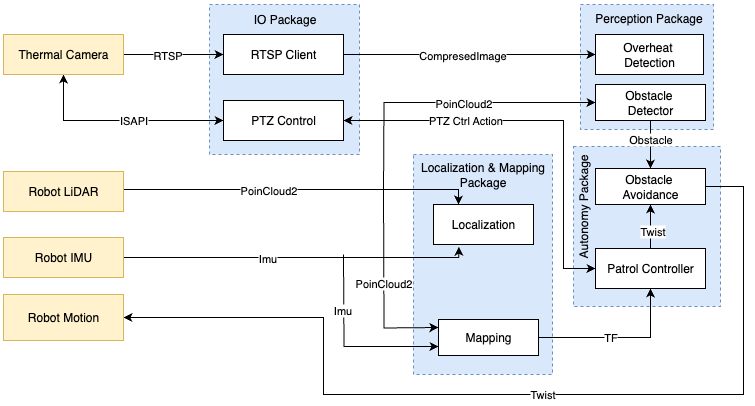
\includegraphics[width=0.8\textwidth]{Init/gambar/diagram_sistem_gusdar.png}
    \caption[Diagram Sistem robot Quadruped untuk Estimasi Posisi Komponen Overheat Pada Gardu Induk Berbasis Kamera Termal]{Diagram Sistem robot Quadruped untuk Estimasi Posisi Komponen Overheat Pada Gardu Induk Berbasis Kamera Termal \cite{Darmawan2025}}
    \label{fig:diagram_sistem_gusdar}																	
\end{figure}

Penelitian yang dilakukan oleh Darmawan \cite{Darmawan2025} mengembangkan sistem pemantauan otonom menggunakan robot \textit{quadruped} untuk mendeteksi kondisi \textit{overheat} pada komponen gardu induk. Arsitektur sistem dari penelitian tersebut, sebagaimana diilustrasikan pada Gambar \ref{fig:diagram_sistem_gusdar}, mengintegrasikan kamera termal dengan model deteksi objek YOLOv8s pada \textit{perception package} yang dioptimasi menggunakan OpenVINO untuk mengenali komponen kelistrikan, serta melakukan analisis suhu aktual secara langsung dari citra termal. Untuk pergerakannya pada \textit{autonomy package}, navigasi robot dikendalikan melalui kombinasi algoritma PID dan \textit{Pure Pursuit} agar dapat mengikuti lintasan patroli secara otonom, didukung oleh penghindaran rintangan menggunakan algoritma Braitenberg. Pada \textit{localization \& mapping package} Proses pemetaan lingkungan tiga dimensi dilakukan menggunakan algoritma SLAM FastLIO2 berdasarkan data LiDAR, dengan lokalisasi yang mengandalkan odometri. Seluruh operasi ini dipantau melalui sebuah \textit{control station} berbasis web yang menerima data telemetri dan aliran video secara waktu nyata melalui protokol WebSocket dan WebRTC. Hasil pengujian menunjukkan bahwa sistem ini berhasil mendeteksi \textit{overheat} dengan akurasi yang tinggi (mAP 0,8554) dan mampu beroperasi secara stabil dalam jarak transmisi hingga 100 meter, menjadikannya solusi inspeksi otonom yang andal.

Sistem ini terbukti andal dalam mendeteksi objek, tetapi mekanisme pengendalian dan navigasinya masih bersifat konvensional dan deterministik (\textit{hard-coded}). Robot hanya mampu bergerak ke lokasi yang koordinatnya telah di program secara eksplisit dalam kode sumber. Sistem ini tidak memiliki fleksibilitas untuk memahami instruksi yang bersifat semantik atau dinamis. Akibatnya, setiap perubahan skenario inspeksi memerlukan pemrograman ulang oleh ahli teknis, yang tidak efisien untuk penerapan lapangan yang dinamis. Selain itu, ketergantungan pada pemantauan telemetri manual masih membebankan beban kognitif yang tinggi pada operator.

\subsection{Interaksi Robot Manusia Berbasis \textit{Large Language Model} untuk Pembuatan \textit{Movement Plan} pada Robot \textit{Quadruped-legged}}

\begin{figure}[H]
    \centering
    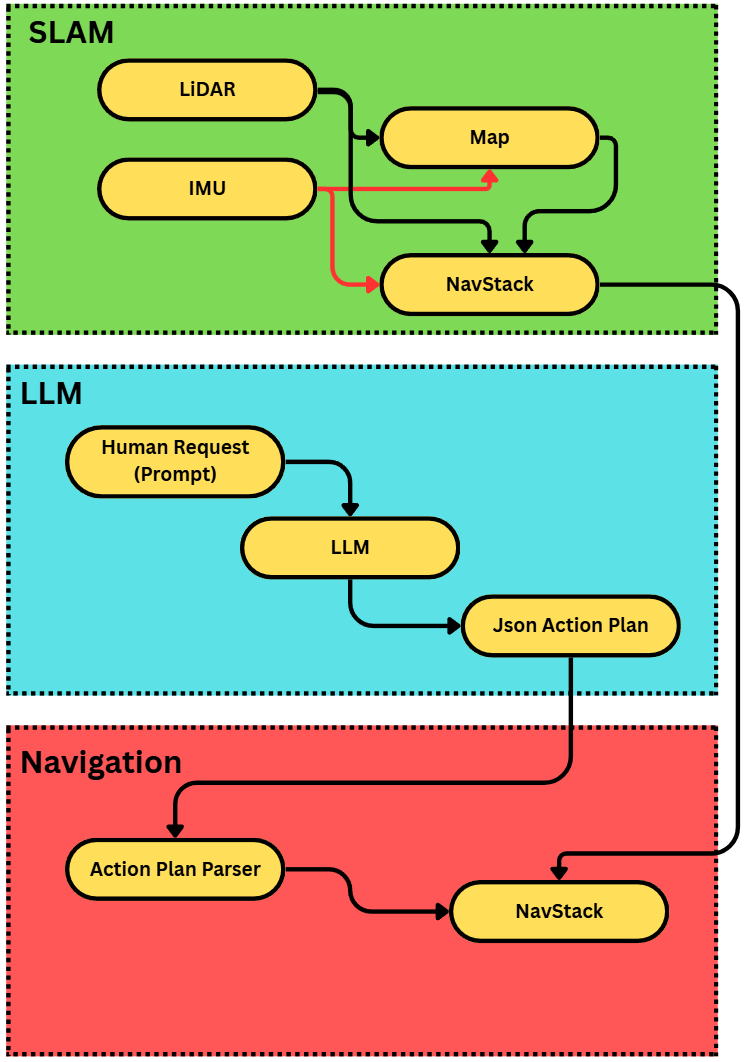
\includegraphics[width=0.5\textwidth]{Init/gambar/diagram_siste_vincent.png}
    \caption[Diagram Sistem Robot Quadruped untuk Interaksi Robot Manusia Berbasis Large Language Model untuk Pembuatan Movement Plan pada Robot Quadruped-legged]{Diagram Sistem Robot Quadruped untuk Interaksi Robot Manusia Berbasis Large Language Model untuk Pembuatan Movement Plan pada Robot Quadruped-legged \cite{Mahendra2024}}
    \label{fig:diagram_sistem_vincent}																	
\end{figure}

Di sisi lain, pendekatan berbeda dilakukan oleh Mahendra \cite{Mahendra2024} yang merancang sistem interaksi manusia-robot berbasis bahasa alami agar robot \textit{quadruped} dapat menyusun rencana pergerakan secara otonom. Arsitektur aliran data sistem tersebut, sebagaimana diilustrasikan pada Gambar \ref{fig:diagram_sistem_vincent}, mengelompokkan fungsionalitas ke dalam tiga modul utama, modul SLAM, modul pemrosesan bahasa (LLM), dan modul Navigasi. Penelitian ini menggunakan robot Jueying Lite 3 Pro yang dilengkapi sensor LiDAR Leishen C16, dengan pemetaan lingkungan menggunakan algoritma SLAM Fast-LIO. Peta yang dihasilkan kemudian dimodifikasi secara manual untuk menutupi batasan sensor, seperti menambahkan dinding virtual pada kaca transparan dan area tangga darurat. Sebagai pusat pemrosesan bahasa, sistem ini mengandalkan API Google Gemini yang diberikan instruksi khusus (\textit{prompt engineering}) mengenai lokasi target (\textit{waypoint}) dan batasan robot. LLM akan merespons perintah dari pengguna, baik berupa teks maupun suara melalui aplikasi web lokal berbasis Flask, dengan menghasilkan dokumen JSON yang berisi urutan perintah navigasi spesifik (seperti goto, halt, searchlab901, dan errmsg). Perintah errmsg didesain sebagai mekanisme keamanan agar LLM menolak permintaan yang tidak masuk akal atau membahayakan robot. Perintah JSON tersebut kemudian diterjemahkan oleh sebuah skrip \textit{parser} menjadi aksi navigasi yang dieksekusi oleh \textit{Navigation Stack} pada ROS. Evaluasi sistem menunjukkan bahwa LLM memiliki tingkat keberhasilan penyusunan rencana sebesar 85\% secara keseluruhan, bahkan mencapai 100\% pada instruksi kompleks maupun penanganan kegagalan. Kinerja navigasi robot juga sangat tinggi dengan rata-rata keberhasilan eksekusi mencapai 96,5\% dari 80 percobaan melintasi berbagai zona, di mana kegagalan kecil murni disebabkan oleh kendala perangkat keras fisik (seperti \textit{overheat} pada motor kaki). Hal ini membuktikan keandalan sistem dalam memproses instruksi percakapan sehari-hari menjadi logika navigasi JSON secara presisi.

Penelitian ini menawarkan fleksibilitas dalam input perintah dibandingkan metode konvensional, tetapi kelemahan mendasarnya terletak pada mekanisme eksekusi tugasnya yang bersifat menyeluruh. Sistem dirancang untuk menghasilkan seluruh rangkaian jalur navigasi di awal dan mengeksekusinya hingga selesai tanpa jeda. Desain alur kerja seperti ini membuat sistem tidak memiliki kemampuan untuk memvalidasi setiap tahapan pergerakan secara bertahap. Ketiadaan umpan balik di tengah misi ini menyebabkan hilangnya kemampuan operator untuk melakukan intervensi guna memodifikasi rencana di tengah jalan, padahal kontrol tersebut diperlukan untuk menyesuaikan strategi dengan kondisi lapangan yang berubah serta memastikan hasil setiap tahapan telah memenuhi standar yang diinginkan sebelum robot melanjutkan ke langkah berikutnya.

\section{Dasar Teori}

Bagian ini menguraikan berbagai landasan konsep, teknologi, dan kerangka teori yang menjadi pilar utama dalam pengembangan sistem pada penelitian ini. Keseluruhan teori ini digunakan untuk membangun pemahaman yang utuh mengenai bagaimana setiap komponen, baik dari sisi perangkat lunak maupun perangkat keras, saling terintegrasi dalam membangun arsitektur sistem inspeksi yang otonom dan adaptif.

\subsection{Lite3 \textit{Quadruped Robot}}

\begin{figure}[H]
    \centering
    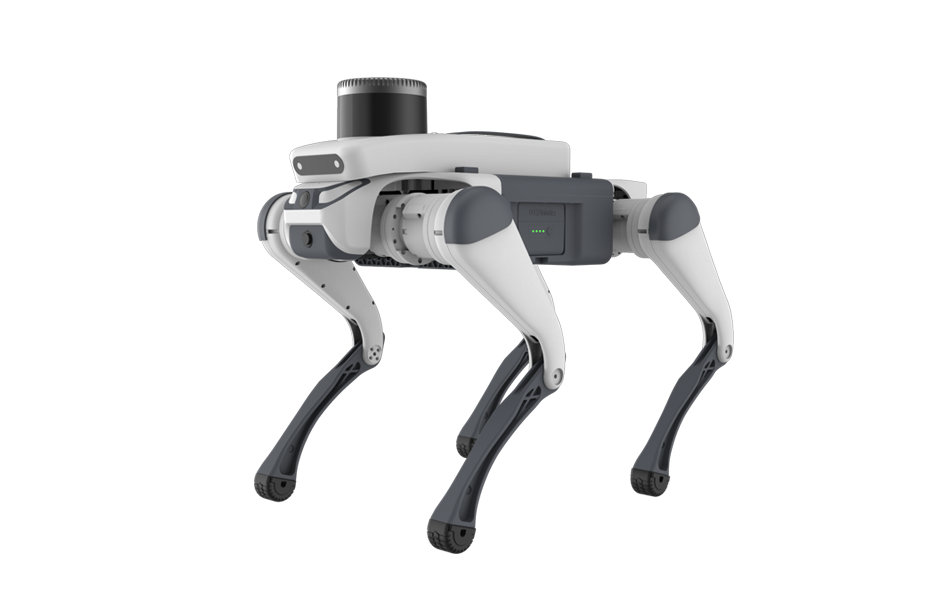
\includegraphics[width=0.5\textwidth]{Init/gambar/lite3.png}
    \caption[Robot Jueying Lite3]{Robot Jueying Lite3 \cite{maverick2026lite3}}
    \label{fig:lite3}
\end{figure}

Gambar \ref{fig:lite3} menunjukkan wujud fisik platform robot Jueying Lite3. Robot \textit{quadruped} merupakan kategori robot yang terinspirasi oleh mekanisme lokomosi hewan berkaki empat, mengintegrasikan desain mekanik, teori kontrol, dan kecerdasan buatan untuk beroperasi di lingkungan yang sulit dijangkau atau berbahaya bagi manusia \cite{li2025quadruped}. Konfigurasi berkaki empat menawarkan keseimbangan optimal antara mobilitas dan stabilitas, menjadikannya lebih stabil dibandingkan robot \textit{bipedal} (berkaki dua) sekaligus lebih lincah dan efisien secara energi dibandingkan robot \textit{hexapod} (berkaki enam) \cite{li2025quadruped}. Kemampuan adaptasi terhadap medan yang tidak rata, tangga, dan permukaan tidak terstruktur menjadikan robot \textit{quadruped} sangat cocok untuk aplikasi inspeksi infrastruktur, pemantauan lingkungan berbahaya, serta skenario pencarian dan penyelamatan di mana kendaraan beroda konvensional tidak dapat dioperasikan \cite{halder2023construction}.

Jueying Lite3 adalah platform robot \textit{quadruped} yang dikembangkan oleh DEEPRobotics dengan keperluan untuk riset dan aplikasi lapangan. DEEPRobotics merancang Lite3 dalam beberapa varian untuk memenuhi kebutuhan yang berbeda, yaitu Lite3 Basic yang merupakan robot anjing dengan kemampuan dasar, Lite3 Venture yang menambahkan konektivitas ethernet dan masukan daya eksternal, Lite3 Pro yang merupakan varian Venture dengan tambahan \textit{mini PC} di atasnya dan kamera kedalaman (\textit{depth camera}) untuk keperluan pengembangan, serta Lite3 Pro LiDAR yang merupakan varian Pro dengan tambahan sensor LiDAR. Salah satu keunggulan utama platform ini terletak pada keterbukaan arsitekturnya. Lite3 memiliki sistem perangkat lunak yang bersifat terbuka (\textit{open source}) sehingga pengembang dapat mengintegrasikan sensor tambahan, mengganti tumpukan perangkat lunak navigasi, atau menghubungkan sistem kecerdasan buatan eksternal tanpa perlu merombak desain dasar robot. Dalam penelitian ini, keterbukaan sistem tersebut dimanfaatkan untuk mengintegrasikan navigasi berbasis ROS dan agen LLM secara penuh ke dalam platform Lite3.

Secara arsitektur perangkat keras, khususnya pada varian Lite3 Pro LiDAR, robot ini dibangun di atas dua unit komputasi utama yang saling terhubung sebagaimana ditunjukkan pada Gambar \ref{fig:hardware_architecture}. Kedua unit tersebut adalah \textit{Motion Host} yang menangani kendali lokomosi dan \textit{Perception Host} yang mengelola pemrosesan data sensor. Keduanya dihubungkan melalui sebuah \textit{Router/Switch} internal untuk komunikasi data di dalam badan robot. 

\begin{figure}[H]
    \centering
    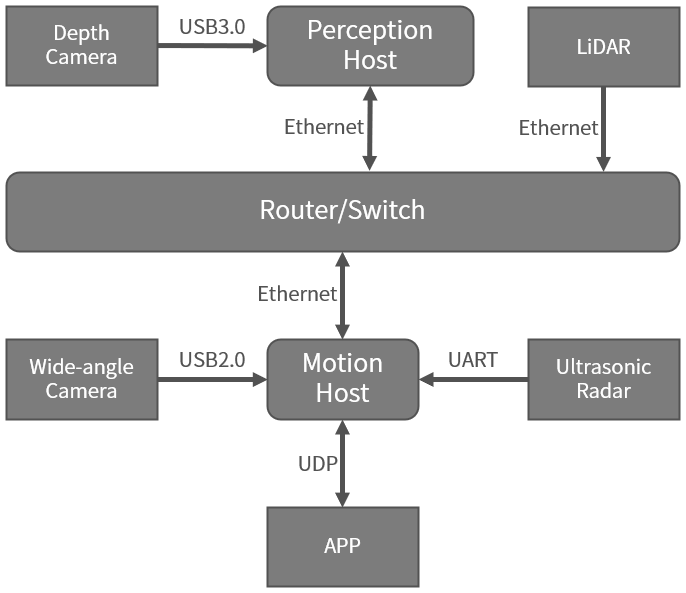
\includegraphics[width=0.5\textwidth]{Init/gambar/hardware_architecture.png}
    \caption[Arsitektur perangkat keras robot Lite3]{Arsitektur perangkat keras robot Lite3 \cite{deeprobotics2024motion}}
    \label{fig:hardware_architecture}
\end{figure}

\subsubsection{\textit{Motion Host}}
\textit{Motion Host} pada Lite3 bertanggung jawab atas seluruh aspek lokomosi fisik robot, meliputi koordinasi sendi, keseimbangan dinamis, dan perencanaan pola langkah (\textit{gait planning}). Sistem ini dikendalikan oleh prosesor berarsitektur ARM (RK3588) yang mampu menjalankan algoritma kontrol gerak berfrekuensi tinggi \cite{deeprobotics2024motion}. Setiap kaki robot terdiri dari tiga sendi aktif, yaitu HipX untuk gerakan abduksi-adduksi pinggul, HipY untuk fleksi-ekstensi pinggul, dan Knee untuk tekukan lutut. Masing-masing sendi digerakkan oleh motor DC berdaya tinggi yang dipasangkan dengan \textit{reducer} presisi dan \textit{absolute encoder} untuk memastikan ketepatan posisi sudut. Sistem ini juga dilengkapi mekanisme proteksi otomatis berupa penghentian gerakan saat suhu motor melebihi ambang batas (\textit{overtemperature protection}) dan deteksi kondisi jatuh (\textit{fall down protection}) yang secara langsung memutus perintah gerak demi keselamatan perangkat.

\subsubsection{\textit{Perception Host}}
\textit{Perception Host} pada Lite3 berfungsi sebagai indera utama yang menyediakan data spasial dan visual agar robot dapat memahami lingkungan di sekitarnya. Subsistem ini ditenagai oleh unit komputasi NVIDIA Jetson Xavier NX yang menyediakan akselerasi GPU untuk menjalankan algoritma persepsi secara \textit{real-time} \cite{deeprobotics2024perception}. Robot ini dilengkapi dengan dua jenis sensor utama yang bekerja secara komplementer. Sensor pertama adalah kamera kedalaman Intel RealSense D435i yang mampu menghasilkan peta kedalaman (\textit{depth map}) dan citra warna (RGB) secara simultan, menyediakan informasi jarak dan visual dari objek di sekitar robot. Sensor kedua adalah LiDAR 3D yang menghasilkan awan titik (\textit{point cloud}) tiga dimensi beresolusi tinggi untuk pemetaan dan lokalisasi spasial. Kedua sensor ini bekerja bersama untuk memberikan representasi lingkungan yang lengkap, di mana data LiDAR digunakan untuk membangun peta 3D dan menentukan posisi robot melalui algoritma SLAM.

\subsubsection{Komunikasi Antar \textit{Motion Host} dan \textit{Perception Host}}

\begin{figure}[H]
    \centering
    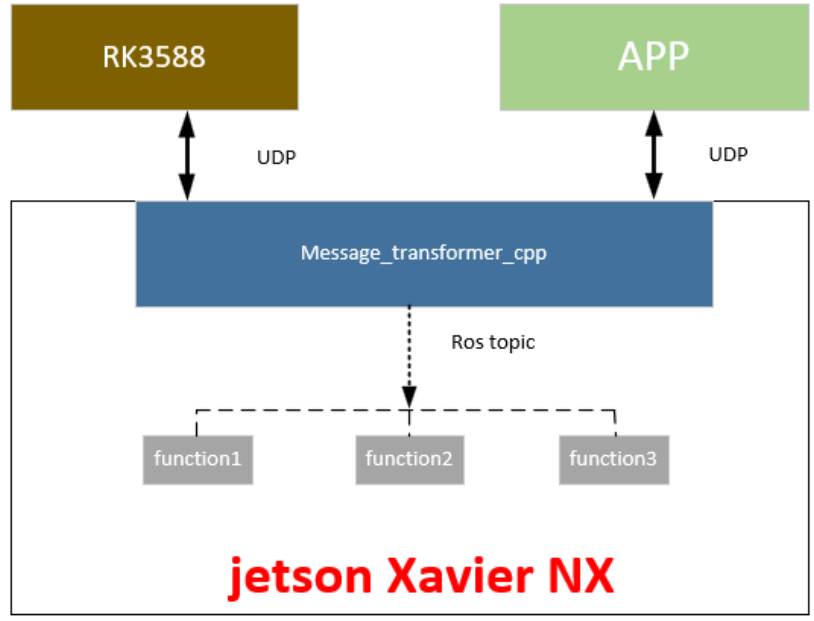
\includegraphics[width=0.6\textwidth]{Init/gambar/lite3_com_diagram.png}
    \caption[Diagram komunikasi antara \textit{Motion Host} dan \textit{Perception Host} pada robot Lite3]{Diagram komunikasi antara \textit{Motion Host} dan \textit{Perception Host} pada robot Lite3 \cite{deeprobotics2024motion}}
    \label{fig:lite3_com_diagram}
\end{figure}

Seperti yang diilustrasikan pada Gambar \ref{fig:lite3_com_diagram}, komunikasi antara \textit{Motion Host} dan \textit{Perception Host} dijalankan melalui protokol \textit{User Datagram Protocol} (UDP) yang bersifat ringan dan berlatensi rendah, sehingga sangat krusial untuk sistem kendali gerak yang membutuhkan respons waktu-nyata (\textit{real-time}). Komunikasi ini bersifat dua arah  dan melibatkan konversi format data di setiap sisinya, karena kedua unit komputasi menggunakan sistem operasi yang berbeda yaitu, \textit{Motion Host} (RK3588) beroperasi di atas sistem operasi \textit{real-time} QNX, sedangkan \textit{Perception Host} (Jetson Xavier NX) beroperasi di atas Linux dengan ekosistem ROS.

Pada arah dari \textit{Motion Host} ke \textit{Perception Host}, data status robot yang dihasilkan oleh sistem QNX pada RK3588 dikemas ke dalam paket UDP dengan format yang kompatibel dengan protokol QNX. Paket-paket ini kemudian diterima oleh modul perantara yang berjalan di Jetson Xavier NX, di mana data tersebut dikonversi dari format QNX menjadi pesan-pesan standar ROS dan diterbitkan ke \textit{topics} yang relevan. Dengan demikian, berbagai modul fungsional yang berjalan di atas ROS pada \textit{Perception Host} dapat mengonsumsi data dari \textit{Motion Host} melalui mekanisme \textit{subscribe} yang standar. Sebaliknya, pada arah dari \textit{Perception Host} ke \textit{Motion Host}, data perintah pergerakan yang dihasilkan oleh navigasi ROS dikemas ulang oleh modul perantara dari format pesan ROS menjadi format UDP yang dapat dipahami oleh sistem QNX pada \textit{Motion Host}. Paket perintah ini kemudian dikirimkan melalui UDP ke RK3588 untuk dieksekusi secara langsung oleh pengendali sendi dan algoritma kendali gerak. 

\subsection{\textit{Robot Operating System} (ROS)}

\textit{Robot Operating System} (ROS) adalah sebuah kerangka kerja (\textit{framework}) perangkat lunak yang fleksibel dan terdistribusi untuk pengembangan sistem robotik. Meskipun bernama sistem operasi, ROS bukanlah sistem operasi dalam artian tradisional seperti Windows atau Linux, melainkan sebuah \textit{middleware} yang berjalan di atasnya. ROS menyediakan layanan standar sistem operasi seperti abstraksi perangkat keras, kontrol perangkat tingkat rendah, implementasi fungsionalitas yang umum digunakan, penyampaian pesan antar proses, dan manajemen paket \cite{quigley2009ros}. Keunggulan utama ROS terletak pada ekosistemnya yang luas, memungkinkan integrasi berbagai driver sensor dan algoritma navigasi tanpa perlu membangun sistem dari nol. Dalam penelitian ini, seluruh infrastruktur perangkat lunak robot \textit{quadruped} dibangun di atas ekosistem ROS sebagai tulang punggung komunikasi dan koordinasi antar-modul, mulai dari persepsi sensor hingga eksekusi perintah navigasi.

\subsubsection{Arsitektur \textit{Node} dan \textit{Master}}
Arsitektur ROS dibangun berdasarkan komponen perangkat lunak independen yang disebut \textit{Nodes}. Setiap \textit{node} adalah sebuah proses komputasi yang bertanggung jawab atas tugas spesifik, seperti mengolah data kamera, merencanakan jalur, atau mengendalikan motor servo. Sifat modular ini memungkinkan tim pengembang untuk mengerjakan berbagai bagian dari sistem robot secara paralel dan independen. Agar \textit{node-node} ini dapat saling menemukan dan berkomunikasi, ROS menggunakan sebuah program inti yang disebut ROS Master (\textit{roscore}). Master menyediakan layanan registrasi nama dan pencarian (\textit{lookup}), yang memungkinkan \textit{node} pengirim dan penerima data untuk membuat koneksi \textit{peer-to-peer}. Arsitektur modular ini memungkinkan sistem robot inspeksi untuk menambahkan atau mengganti modul sensor dan navigasi tanpa harus merombak keseluruhan sistem.

\subsubsection{Mekanisme Komunikasi}

\begin{figure}[H]
    \centering
    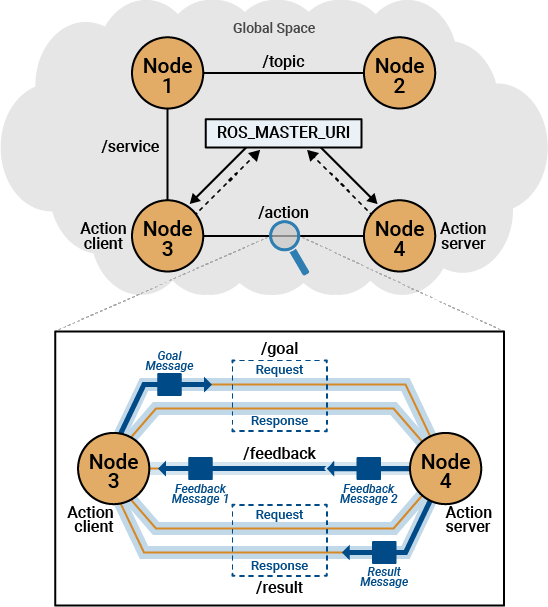
\includegraphics[width=0.6\textwidth]{Init/gambar/ros_actions.png}
    \caption[Diagram komunikasi antar-node dalam ROS]{Diagram komunikasi antar-node dalam ROS \cite{mathworks2025ros}}
    \label{fig:ros_communication}
\end{figure}

Mekanisme alur komunikasi antar-node dalam ROS sebagaimana diilustrasikan pada Gambar \ref{fig:ros_communication} difasilitasi oleh tiga mekanisme utama yang disesuaikan dengan kebutuhan pertukaran data yang berbeda:

\begin{enumerate}
    \item \textbf{Topics:} Mekanisme komunikasi asinkron yang menggunakan model \textit{publish-subscribe}. Sebuah \textit{node} (publisher) menyiarkan pesan ke sebuah \textit{topic} tertentu tanpa perlu mengetahui siapa penerimanya. \textit{Node} lain (subscriber) yang berlangganan ke topik tersebut akan menerima data secara \textit{real-time}. Mekanisme ini ideal untuk aliran data sensor berkelanjutan, seperti data LiDAR atau video stream.
    
    \item \textbf{Services:} Mekanisme komunikasi sinkron yang menggunakan model \textit{request-response}. Sebuah \textit{node} mengirimkan permintaan (\textit{request}) dan menunggu hingga \textit{node} penyedia layanan memprosesnya dan mengirimkan balasan (\textit{response}). Mekanisme ini cocok untuk tugas sesaat yang membutuhkan konfirmasi langsung, seperti menyalakan lampu LED atau mengubah mode operasi robot.
    
    \item \textbf{Actions:} Mekanisme komunikasi yang dirancang untuk tugas jangka panjang yang memerlukan waktu untuk diselesaikan dan membutuhkan umpan balik berkelanjutan. Berbeda dengan \textit{Services} yang memblokir proses hingga selesai, \textit{Actions} memungkinkan robot untuk membatalkan tugas di tengah jalan dan memberikan status progres secara berkala. Ini adalah mekanisme fundamental dalam navigasi robot, misalnya saat robot bergerak dari titik A ke titik B \cite{quigley2009ros}.
\end{enumerate}

\subsubsection{ROS \textit{Navigation Stack}}

\begin{figure}[H]
    \centering
    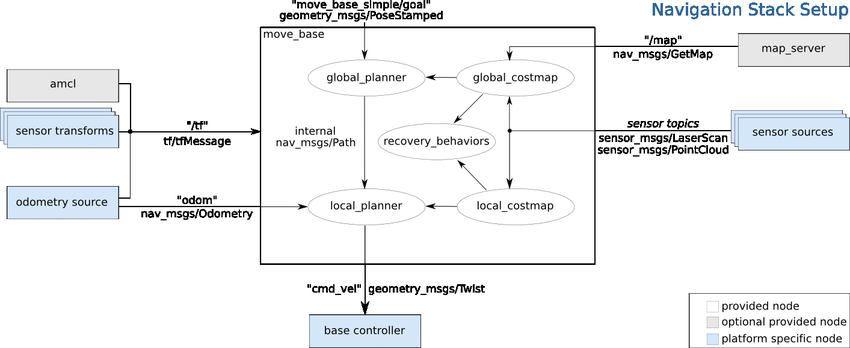
\includegraphics[width=0.8\textwidth]{Init/gambar/ros_nav.png}
    \caption[Diagram arsitektur ROS Navigation Stack]{Diagram arsitektur ROS Navigation Stack \cite{prague2016navstack}}
    \label{fig:ros_nav}
\end{figure}

Sebagaimana diilustrasikan pada Gambar \ref{fig:ros_nav}, fungsionalitas pergerakan otonom di dalam ekosistem ROS difasilitasi oleh kumpulan pustaka dan modul terintegrasi yang dikenal sebagai \textit{Navigation Stack}. Arsitektur navigasi ini berpusat pada \textit{move\_base}, sebuah \textit{node} koordinator yang mengintegrasikan aliran informasi dari berbagai sistem, termasuk \textit{transform tree} (TF) untuk melacak relasi spasial, data peta spasial, pembacaan sensor LiDAR, dan telemetri odometri robot. Ketika \textit{move\_base} menerima sebuah target koordinat tujuan (\textit{goal pose}) dalam bentuk pesan \textit{Action}, ia meneruskan data persepsi tersebut ke modul perencana jalur global (\textit{global planner}) dan lokal (\textit{local planner}) secara bertahap. Hasil akhir dari pemrosesan di dalam \textit{node} navigasi ini adalah pengiriman perintah gerak secara berkala melalui \textit{topic} yang mengatur kecepatan linier dan sudut (\textit{cmd\_vel}). Perintah ini selanjutnya diterjemahkan oleh unit pengendali perangkat keras (\textit{hardware controller}) menjadi putaran motor yang menggerakkan robot menuju tujuannya. Dalam penelitian ini, \textit{Navigation Stack} digunakan sebagai kerangka utama yang mengoordinasikan seluruh proses navigasi robot \textit{quadruped}, mulai dari penerimaan tujuan yang dikirimkan oleh agen LLM hingga eksekusi gerakan fisik di lingkungan pabrik.

\subsubsection{\textit{Rosbridge Suite}}
\textit{Rosbridge Suite} adalah lapisan \textit{middleware} yang dirancang untuk menjembatani komunikasi antara ekosistem ROS dengan aplikasi eksternal yang tidak berbasis ROS, seperti aplikasi antarmuka web atau klien jarak jauh \cite{crick2016rosbridge}. Komponen ini bekerja dengan menyediakan antarmuka \textit{Application Programming Interface} (API) berbasis JSON (\textit{JavaScript Object Notation}) yang dapat diakses melalui standar komunikasi \textit{WebSocket}. Melalui \textit{rosbridge}, aplikasi pihak ketiga dapat melakukan operasi fundamental ROS secara langsung di atas jaringan, seperti mempublikasikan (\textit{publish}) data ke suatu \textit{topic}, berlangganan (\textit{subscribe}) untuk menerima aliran data sensor, atau memanggil layanan (\textit{services}) tanpa perlu menginstal pustaka ROS secara penuh di sisi klien. Dalam arsitektur sistem robot inspeksi yang terhubung ke internet, \textit{rosbridge} memegang peranan esensial sebagai jalur komunikasi utama yang memfasilitasi pengiriman perintah dari \textit{dashboard} kontrol maupun \textit{Large Language Model}, sekaligus menyalurkan telemetri dan data pandangan robot secara \textit{real-time} kembali ke pengguna.


\subsection{Lokalisasi dan Pemetaan}
Lokalisasi dan pemetaan merupakan kemampuan fundamental yang saling bergantung bagi robot otonom untuk dapat beroperasi dan menavigasi lingkungan yang kompleks secara presisi. Dalam disiplin ilmu robotika, proses memetakan lingkungan sekaligus menentukan posisi robot di dalamnya diistilahkan sebagai \textit{Simultaneous Localization and Mapping} (SLAM). Menurut Thrun dkk. \cite{stachniss2016simultaneous}, SLAM adalah kerangka dasar bagi robot otonom sejati karena mengizinkan sistem untuk memahami lingkungan yang tidak terstruktur tanpa perlu bergantung pada instrumen penentuan posisi eksternal. Secara teknis, proses pemetaan bertugas membangun representasi tata letak rintangan di sekeliling robot berdasarkan data sensor, sementara proses lokalisasi secara terus-menerus menggunakan peta tersebut untuk mengestimasi letak dan arah robot. Gabungan dari kedua kemampuan pemetaan ruang ini menjadi fondasi penting dalam pengembangan proyek robot inspeksi \textit{quadruped}, yang mensyaratkan tersedianya peta 3D lingkungan sebelum sistem dapat menjalankan misi navigasi secara otonom berdasarkan instruksi dari \textit{Large Language Model}.

\subsubsection{\textit{Graph} SLAM}

\begin{figure}[H]
    \centering
    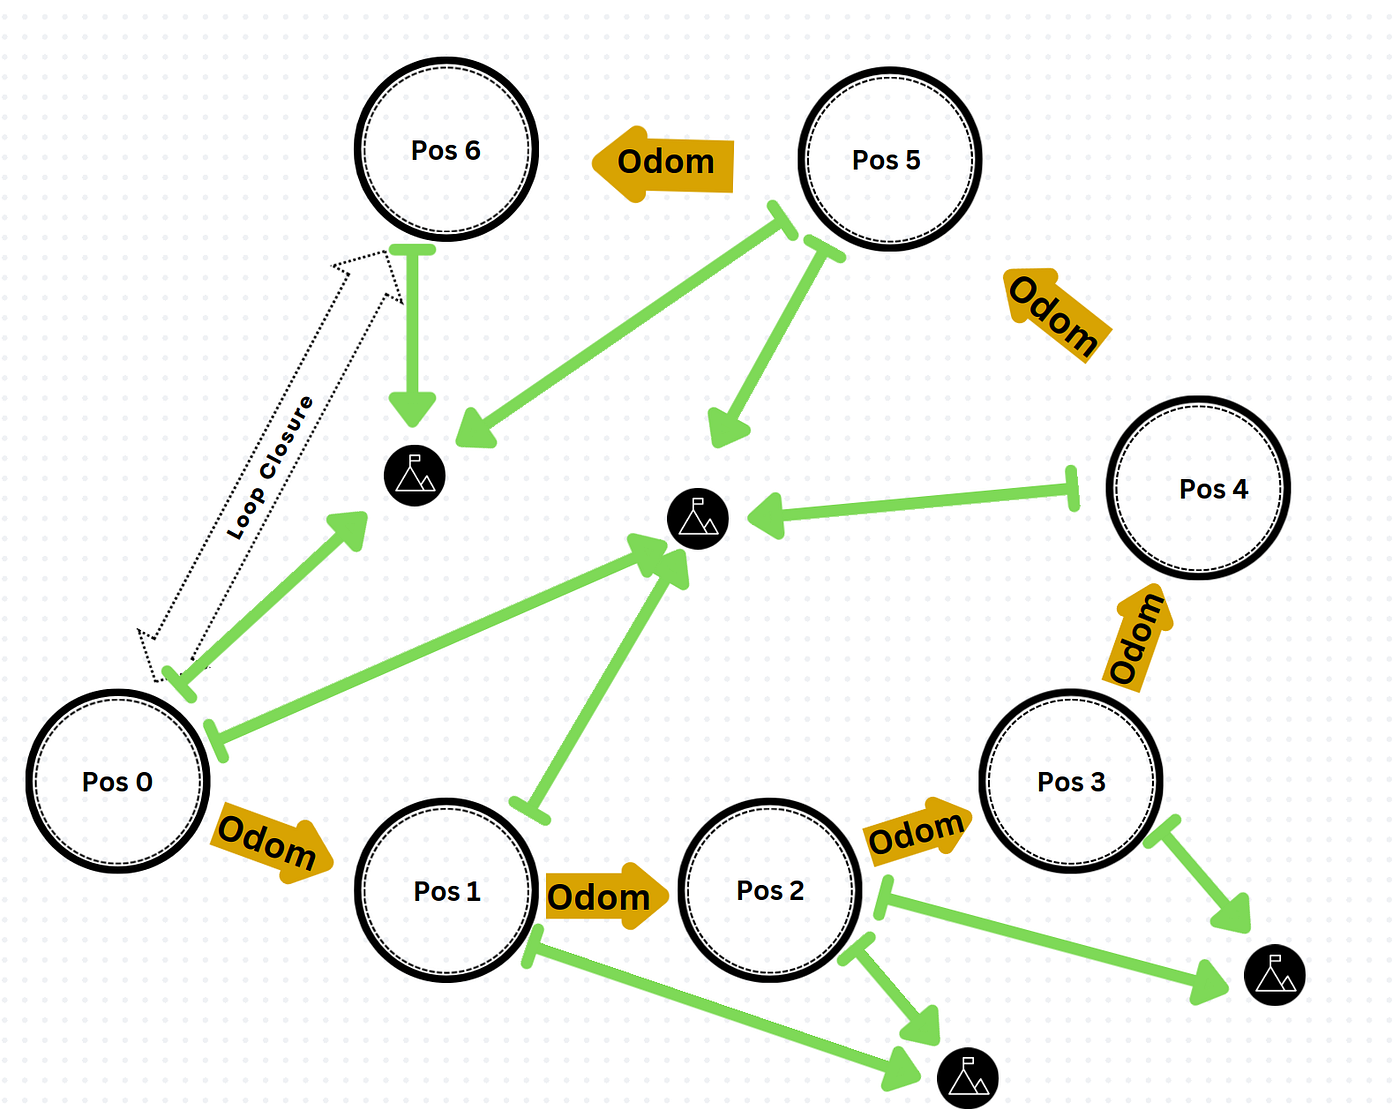
\includegraphics[width=0.65\textwidth]{Init/gambar/graph_slam.png}
    \caption[Diagram Graph SLAM]{Diagram Graph SLAM \cite{rustam2024graphslam}}
    \label{fig:graph_slam}
\end{figure}

Berdasarkan skema pada Gambar \ref{fig:graph_slam}, \textit{Graph SLAM} adalah pendekatan pemetaan yang merepresentasikan riwayat perjalanan robot sebagai sebuah graf posisi (\textit{pose graph}), di mana setiap simpul (\textit{node}) mewakili pose robot pada waktu tertentu dan setiap \textit{edge} mewakili kendala spasial yang diturunkan dari data sensor maupun odometri. Metode ini secara fundamental memformulasikan SLAM sebagai persoalan optimasi graf, di mana akumulasi kesalahan estimasi jarak (\textit{drift}) dapat dikoreksi secara menyeluruh melalui mekanisme pengenalan area berulang (\textit{loop closure}) yang memperbarui seluruh riwayat rute secara konsisten. Dalam konteks implementasi pada sistem berbasis LiDAR, Koide dkk. \cite{koide2019portable} mengembangkan \textit{hdl\_graph\_slam}, sebuah implementasi Graph SLAM yang portabel dan efisien untuk pemetaan 3D menggunakan sensor LiDAR. Implementasi ini memanfaatkan kombinasi algoritma \textit{scan matching} dan optimasi graf untuk menghasilkan peta 3D berkualitas tinggi secara \textit{real-time}. Penggunaan kerangka kerja ini dalam penelitian memastikan bahwa robot \textit{quadruped} dapat menghasilkan peta 3D lingkungan pabrik yang presisi sebagai panduan utama untuk proses penentuan lokasi dan navigasi otonom.

% \subsubsection{Normal Distributions Transform (NDT)}
% \textit{Normal Distributions Transform} (NDT) merupakan algoritma pencocokan pemindaian (\textit{scan matching}) yang efisien karena menyelaraskan dua himpunan \textit{point cloud} dengan memodelkannya ke dalam probabilitas distribusi spasial. Biber dan Stra{\ss}er \cite{biber2003normal} mengemukakan rumusan NDT yang bekerja dengan membagi ruang ke dalam sel-sel berukuran tetap dan merepresentasikan titik-titik permukaan di dalam setiap sel menggunakan matriks kovariansi dan nilai rata-rata dari distribusi Gaussian. Melalui implementasi paralelisasi komputasi (\textit{multi-threading}), pemetaan probabilitas ini menghilangkan kebutuhan komputasi berat untuk mencari korespondensi individual dari titik-ke-titik secara persis saat meregistrasikan sensor LiDAR baru ke \textit{global map} 3D. Kemampuan matematis NDT yang efisien memberikan kepastian perhitungan \textit{pose} (posisi dan orientasi) secara \textit{real-time}, sehingga robot selalu dapat mengeksekusi manuver navigasi spasialnya tanpa lag komputasi yang berbahaya.

\subsubsection{\textit{Fast-Generalized Iterative Closest Point} (Fast-GICP)}
\textit{Fast-Generalized Iterative Closest Point} (Fast-GICP) adalah algoritma optimasi dari GICP standar yang difokuskan untuk mengakselerasi tahap kalkulasi matriks transformasi pada registrasi \textit{point cloud} 3D. Koide dkk. \cite{koide2021voxelized} mengembangkan varian efisien \textit{Fast-GICP} yang menerapkan paralelisasi dan struktur data berbasis \textit{voxel} sehingga mampu mempertahankan keakuratan yang ekuivalen dengan GICP standar sembari menekan latensi komputasi secara masif. Di dalam lapisan persepsi robot, algoritma ini menangani data \textit{point cloud} berskala besar dengan lebih ringkas karena struktur voksel secara dramatis meminimalkan redundansi pencarian titik terdekat (\textit{nearest-neighbor matching}) yang secara konvensional menjadi \textit{bottleneck} komputasi. Pemanfaatan kapabilitas pencocokan super cepat dari \textit{Fast-GICP} ini berdampak langsung pada modul perencanaan (\textit{planning}), yang memampukan robot \textit{quadruped} untuk mengenali letak dirinya secara instan dan bereaksi lincah terhadap rintangan di area pabrik industri.

\subsection{Navigasi}
Sistem navigasi otonom adalah kapabilitas pengambilan keputusan yang memungkinkan robot untuk menentukan dan mengeksekusi lintasan pergerakan paling aman dari titik awal menuju lokasi target. Pada arsitektur operasional robot tingkat lanjut, proses navigasi dikendalikan melalui pengontrol terpusat yang bersifat hierarkis \cite{quigley2009ros}. Sistem ini beroperasi dengan memecah permasalahan lintasan menjadi dua lapisan independen: \textit{Global Planner} untuk menentukan jalur keseluruhan secara makro, dan \textit{Local Planner} untuk menerjemahkan jalur tersebut menjadi perintah kendali motor reaktif. Pembagian kerja ini memisahkan perhitungan rute jarak jauh yang hanya membutuhkan analisis peta statis, dari kebutuhan kalkulasi menghindar rintangan (\textit{obstacle avoidance}) secara refleksif yang sangat sensitif terhadap latensi waktu. Koordinasi antara kedua tingkat perencanaan ini sangat dibutuhkan agar robot \textit{quadruped} dapat melaksanakan inspeksi ke berbagai titik komponen secara efisien dan aman.

\subsubsection{Algoritma \textit{Shortest Path} Dijkstra sebagai \textit{Global Planner}}
\textit{Global Planner} adalah perencana jalur tingkat makro yang bertugas mengkalkulasi lintasan rute terpendek secara absolut di atas referensi peta statis (\textit{global map}). Untuk melakukan kalkulasi rute, lapisan ini seringkali memanfaatkan algoritma \textit{shortest path} seperti Dijkstra \cite{dijkstra2022note}, yaitu metode matematis yang menjamin penemuan rute terpendek dari satu titik awal ke semua titik lain pada peta. Algoritma ini membaca \textit{grid cells} dari peta, lalu menghitung jarak kumulatif dari setiap area yang belum dikunjungi hingga menemukan titik akhir tujuan. Penggunaan Dijkstra dinilai ideal dibandingkan algoritma alternatif seperti \textit{A-Star} (A*) apabila tujuannya adalah mendapatkan jaminan jalur yang paling mulus (\textit{smooth}) dan stabil dari berbagai arah, meskipun membutuhkan proses perhitungan awal yang sedikit lebih berat. Jaminan rute terpendek yang dihasilkan algoritma ini memastikan bahwa robot dapat bergerak seefisien mungkin tanpa membuang daya baterai.

Secara matematis, pembaruan jarak minimum pada algoritma Dijkstra untuk setiap simpul $v$ yang berdekatan dengan simpul $u$ diformulasikan sebagai berikut:

\begin{equation}
d(v) = \min(d(v), d(u) + w(u, v))
\label{eq:dijkstra}
\end{equation}

di mana $d(v)$ adalah jarak terpendek sementara dari titik awal ke simpul $v$, $d(u)$ adalah jarak terpendek yang telah diketahui ke simpul $u$, dan $w(u, v)$ adalah bobot atau jarak lintasan dari simpul $u$ ke simpul $v$.

\subsubsection{\textit{Timed Elastic Band} sebagai \textit{Local Planner}}
\textit{Timed Elastic Band} (TEB) adalah algoritma \textit{Local Planner} tingkat mikro yang secara dinamis memodifikasi trayektori jalur global untuk menghindari tabrakan secara \textit{real-time}. Diperkenalkan oleh R{\"o}smann dkk. \cite{rosmann2012trajectory}, pendekatan TEB bekerja dengan cara mengoptimalkan jalur secara terus-menerus menyerupai karet elastis yang dapat ditarik atau didorong menjauhi rintangan, sembari sangat mempertimbangkan batasan kinematik dan dinamik dari robot otonom. Secara konseptual, TEB diatur agar mampu menyesuaikan diri dengan cara berjalan fisik dari robot, baik itu gaya gerak segala arah (\textit{holonomik}) maupun terbatas (\textit{non-holonomik}). Algoritma ini secara langsung memperhitungkan batas kemampuan perangkat seperti batas percepatan maksimum, batas kecepatan maju, hingga batas radius putaran. Dengan perhitungan ini, pergerakan robot saat menghindari objek bergerak akan selalu terlihat halus dan tetap seimbang. Penerapan sistem lapis pelindung TEB ini memastikan bahwa ketika program AI mengirimkan urutan tujuan yang sulit, robot tetap bisa bereaksi dengan gesit dan berbelok dengan aman, sekalipun berada di area kerja yang ramai dengan aktivitas.

Secara matematis, TEB memformulasikan masalah perencanaan lintasan lokal sebagai persoalan optimasi multi-objektif. Fungsi objektif yang diminimalkan merupakan kombinasi berbobot dari berbagai fungsi \textit{cost} kendala kinematik dan spasial:

\begin{equation}
f(\mathbf{B}) = \sum_{k} \gamma_k f_k(\mathbf{B})
\label{eq:teb_objective}
\end{equation}

di mana $\mathbf{B}$ merepresentasikan urutan konfigurasi pose robot dan interval waktu antar pose, $f_k(\mathbf{B})$ adalah fungsi-fungsi \textit{cost} spesifik (seperti optimasi waktu tempuh, jarak dari rintangan, dan pemenuhan batasan kecepatan), serta $\gamma_k$ adalah parameter bobot untuk masing-masing fungsi \textit{cost} tersebut.

\subsection{\textit{Model Context Protocol} (MCP)}

\begin{figure}[H]
    \centering
    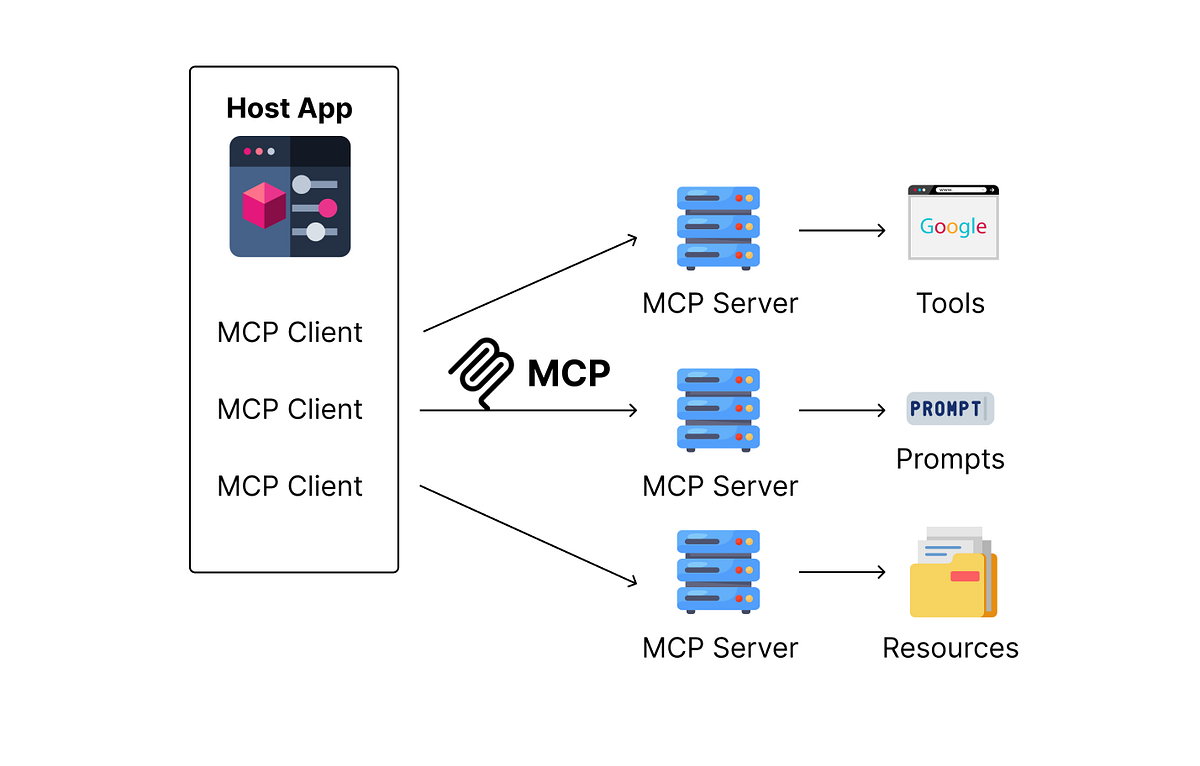
\includegraphics[width=0.8\textwidth]{Init/gambar/mcp.png}
    \caption[Diagram arsitektur MCP]{Diagram arsitektur MCP \cite{zhao2025mcp}}
    \label{fig:mcp}
\end{figure}

Seperti yang ditunjukkan oleh arsitektur pada Gambar \ref{fig:mcp}, \textit{Model Context Protocol} (MCP) adalah sebuah antarmuka terstandarisasi yang dirancang untuk memungkinkan interaksi yang lancar antara model AI dengan \textit{tools} dan sumber daya eksternal. Tujuan utama protokol ini adalah mengatasi masalah isolasi data dan memfasilitasi interoperabilitas di antara berbagai sistem yang berbeda. Sebelum adanya MCP, pengembang harus membuat koneksi API secara manual untuk setiap layanan eksternal (n-to-n connection). Sebaliknya, MCP menyediakan sebuah lapisan abstraksi universal, di mana aplikasi AI (sebagai MCP Client) dapat berkomunikasi dengan berbagai \textit{tools} melalui perantara yang disebut MCP Server, mengubah pola koneksi menjadi 1-to-n yang lebih efisien \cite{hou2025model}.

\subsubsection{Komponen MCP} Berdasarkan tinjauan oleh Hou et al. \cite{hou2025model}, arsitektur MCP dibangun di atas tiga komponen fundamental yang saling berinteraksi secara sinergis. Komponen pertama adalah MCP Host, yang merupakan aplikasi utama tempat model AI dijalankan, seperti \textit{Integrated Development Environment} (IDE) atau aplikasi antarmuka obrolan. Host ini bertindak sebagai wadah (\textit{container}) bagi proses AI. Di dalam ekosistem tersebut, terdapat MCP Client yang berfungsi sebagai jembatan komunikasi di dalam Host. Client bertanggung jawab penuh untuk mengelola koneksi 1:1 dengan Server, mengirimkan permintaan pengguna, dan menangani respons balik. Dalam penelitian ini, peran tersebut dijalankan oleh skrip Python yang mengelola sesi obrolan. Komponen terakhir adalah MCP Server, yang bertugas mengekspos kemampuan teknis kepada AI. Server ini menyediakan tiga jenis primitif utama, yaitu \textit{Tools} yang merupakan fungsi eksekusi seperti navigasi robot atau API query, \textit{Resources} yang berisi data yang dapat dibaca seperti file log atau database, serta \textit{Prompts} yang menyediakan templat instruksi yang telah ditentukan sebelumnya. Dengan arsitektur ini, MCP memungkinkan model AI untuk secara dinamis menemukan dan memilih alat yang dibutuhkan sesuai dengan konteks tugas yang sedang dihadapi \cite{singh2025survey}.

\subsubsection{Protokol Transportasi MCP} Komunikasi antara Client dan Server dalam ekosistem MCP difasilitasi oleh dua mekanisme transportasi standar yang dipilih berdasarkan arsitektur jaringan sistem. Metode pertama adalah Standard Input/Output (stdio), yang digunakan khusus untuk komunikasi lokal di mana Client meluncurkan Server sebagai sub-proses. Metode ini menawarkan keunggulan berupa latensi yang sangat rendah dan tingkat keamanan yang tinggi karena proses tidak terekspos ke jaringan luar. Sebagai alternatif untuk komunikasi jarak jauh dan terdistribusi, digunakan mekanisme HTTP dengan Server-Sent Events (SSE). Dalam mode ini, Server berjalan sebagai layanan web independen, di mana Client mengirimkan perintah melalui HTTP POST dan menerima pembaruan atau notifikasi kejadian (events) secara \textit{real-time} melalui SSE. Metode kedua inilah yang diterapkan dalam penelitian ini untuk menghubungkan antarmuka obrolan dengan server robot yang berjalan di lingkungan terisolasi (Docker).

\subsection{\textit{Large Language Models} (LLM)}
\textit{Large Language Models} (LLM) merupakan model komputasi canggih yang dibangun di atas arsitektur jaringan saraf tiruan, khususnya arsitektur \textit{Transformer}, yang dilatih menggunakan korpus data teks dalam skala masif. Kemampuan fundamental LLM terletak pada proses prediksi \textit{token} atau kata berikutnya dalam sebuah urutan (\textit{next-token prediction}). Proses ini memungkinkan model untuk memelajari tata bahasa, konteks, penalaran, dan pengetahuan umum dari data latihnya secara mendalam. Arsitektur \textit{Transformer}, dengan mekanisme \textit{self-attention}, sangat efektif dalam menangani dependensi jarak jauh (\textit{long-range dependencies}) dalam teks, sehingga model dapat memahami konteks dari sebuah kalimat atau paragraf secara utuh dan komprehensif \cite{chang2024survey}. Dalam penelitian ini, LLM berperan sebagai otak utama agen robot yang menerjemahkan instruksi bahasa alami dari operator menjadi rangkaian perintah navigasi dan inspeksi yang dapat dieksekusi secara langsung oleh sistem robotik.

\subsubsection{\textit{Agentic} AI}
Perkembangan terbaru dalam bidang kecerdasan buatan telah mendorong evolusi \textit{Large Language Models} (LLM) dari sekadar mesin pemroses teks pasif menjadi \textit{autonomous agents} yang mampu berinteraksi secara aktif dengan lingkungannya demi mencapai tujuan tertentu. Xi et al. \cite{xi2025rise} mendefinisikan agen berbasis LLM sebagai sistem yang memanfaatkan model bahasa besar sebagai pengendali utama atau otak untuk mempersepsikan lingkungan, mengambil keputusan, dan mengeksekusi tindakan. Berbeda dengan LLM standar yang kemampuannya terbatas pada menghasilkan teks atau saran konseptual, Agentic AI memanfaatkan pemahaman semantiknya sebagai landasan untuk merumuskan dan mengeksekusi tindakan nyata. Kemampuan inilah yang memungkinkan sistem untuk tidak sekadar merespons instruksi abstrak secara pasif, melainkan beradaptasi dengan skenario yang tidak terduga melalui interaksi otonom menggunakan alat bantu (\textit{tools}) eksternal.

Secara arsitektural, Wang et al. \cite{wang2024survey} merumuskan kerangka kerja \textit{agent} ke dalam empat komponen fundamental yang saling terintegrasi, yaitu profil agen, memori, perencanaan, dan tindakan. Komponen perencanaan (\textit{planning}) memainkan peran krusial dalam sistem robotik, di mana \textit{agent} harus memecah instruksi tingkat tinggi yang kompleks menjadi serangkaian sub-tugas yang dapat dieksekusi atau \textit{Chain of Thought}. Kemampuan ini memungkinkan \textit{agent} untuk melakukan dekomposisi masalah dan refleksi diri, sehingga dapat memperbaiki rencana jika menemui kegagalan saat eksekusi. Sementara itu, komponen memori memungkinkan \textit{agent} untuk menyimpan riwayat interaksi dan pengetahuan prosedural, menciptakan pengalaman pengguna yang kontinu dan kontekstual. Dalam penelitian ini, arsitektur \textit{agentic} diimplementasikan melalui \textit{agent} LLM yang memiliki akses langsung ke \textit{tools} navigasi dan inspeksi robot melalui MCP Server.

\subsubsection{Penggunaan \textit{Tools} dan \textit{Model Context Protocol} (MCP)}
Salah satu kapabilitas LLM modern yang paling signifikan adalah kemampuan \textit{tool use} atau penggunaan alat. Dalam ekosistem pengembangan \textit{agent}, \textit{tools} dalam konteks \textit{Model Context Protocol} (MCP) didefinisikan sebagai kapabilitas eksekusi yang diekspos oleh server, yang memberdayakan LLM untuk melakukan aksi nyata, berinteraksi dengan sistem eksternal, dan menjalankan operasi dinamis di luar sekadar memberikan respons teks statis \cite{singh2025survey}.

Berbeda dengan sumber data pasif, \textit{tools} dirancang untuk pemanggilan aktif oleh model. Mekanisme ini secara signifikan memperluas fungsionalitas \textit{agentic} dari sistem berbasis LLM. Ketika LLM mendeteksi bahwa permintaan pengguna memerlukan interaksi sistem (seperti mengambil data sensor atau menggerakkan robot), model akan menghasilkan \textit{output} terstruktur yang sesuai dengan skema JSON yang telah didefinisikan. Skema ini merinci parameter input dan validasi untuk memastikan eksekusi perintah yang aman dan presisi pada sistem target \cite{singh2025survey}.

\subsubsection{\textit{Multimodal Large Language Models} (MLLM)}
Sejalan dengan kebutuhan interaksi yang lebih kompleks, LLM telah berevolusi menjadi \textit{Multimodal Large Language Models} (MLLM). Ekstensi arsitektural ini memampukan model bahasa untuk tidak hanya memproses dan memahami teks, tetapi juga menerima berbagai jenis modalitas data lain seperti \textit{image}, video, dan audio sebagai masukannya \cite{yin2024survey}. Proses perpaduan ragam data ini diwujudkan melalui komponen enkoder khusus (seperti \textit{vision encoder}) yang bertugas mengekstraksi fitur visual, lalu menggunakan mekanisme penyelarasan (\textit{alignment}) untuk memetakan representasi fitur tersebut ke dalam ruang laten bahasa yang sama. Dalam ranah robotika, kehadiran MLLM menawarkan lompatan kapabilitas persepsi yang besar. Alih-alih bergantung pada sistem penglihatan komputer (\textit{computer vision}) tradisional yang sempit kemampuannya, robot kini dapat memahami dan menalar apa yang dilihat oleh kameranya yang kemudian dijelaskan kembali secara kontekstual menggunakan bahasa alami. Hal ini memungkinkan robot inspeksi untuk memproses konteks visual lingkungannya secara utuh guna melakukan analisis mendalam terhadap objek-objek inspeksi.


\subsection{Interaksi Manusia-Robot (\textit{Human-Robot Interaction})}
\textit{Human-Robot Interaction} (HRI) merupakan bidang studi multidisiplin yang berfokus pada perancangan, evaluasi, dan pemahaman mekanisme interaksi antara manusia dan robot dengan tujuan utama menciptakan kolaborasi yang aman, efisien, dan alami. Dalam spektrum metode interaksi yang ada, penggunaan bahasa alami (\textit{natural language}) dianggap sebagai salah satu pendekatan paling menjanjikan karena meminimalisasi hambatan komunikasi, memungkinkan pengguna untuk berinteraksi dengan robot tanpa memerlukan pelatihan teknis khusus atau pemahaman antarmuka grafis yang rumit \cite{mavridis2015review}. Dengan memampukan robot untuk memproses instruksi tingkat tinggi dalam bahasa sehari-hari seperti perintah "periksa area di sebelah kanan", sistem HRI berbasis bahasa alami dapat secara signifikan menurunkan beban kognitif operator. Hal ini memungkinkan perhatian operator dialihkan dari mekanisme kontrol ke tujuan strategis misi.

Efektivitas sebuah sistem HRI tidak hanya diukur dari kemampuan robot dalam menerjemahkan perintah input, tetapi juga dari kapasitasnya dalam memberikan umpan balik yang komprehensif kepada operator. Kemampuan robot untuk melaporkan status operasional, intensi pergerakan, atau temuan inspeksi secara verbal maupun sangat krusial dalam membangun pemahaman situasi. Dalam konteks tugas inspeksi industri, transparansi informasi ini memastikan operator memahami apa yang sedang dipersepsikan oleh robot secara \textit{real-time}. Hal ini mengubah peran operator dari sekadar pengendali alat menjadi supervisor misi, di mana kompleksitas penerjemahan sinyal teknis dan pelaporan status ditangani secara otonom oleh sistem cerdas, yang pada akhirnya mempercepat adopsi teknologi robotik di lingkungan kerja yang kompleks.

Integrasi \textit{Large Language Models} (LLM) ke dalam arsitektur HRI memperkuat hal ini dengan menawarkan fleksibilitas yang tidak dimiliki oleh sistem berbasis \textit{hard-coded}. Berbeda dengan sistem tradisional yang memerlukan perintah spesifik, HRI yang ditenagai oleh LLM mampu menangani ambiguitas bahasa dan menyimpulkan konteks implisit dari instruksi operator. Kemampuan ini sangat relevan untuk robot inspeksi otonom, di mana instruksi sering kali bersifat dinamis dan bergantung pada situasi lingkungan yang tidak terduga.

\subsubsection{Mekanisme \textit{Human-in-the-Loop} (HITL)}
\textit{Human-in-the-Loop} (HITL) adalah sebuah pendekatan dalam sistem otonom dan kecerdasan buatan yang secara eksplisit mengintegrasikan intervensi manusia ke dalam siklus operasional sistem. Dalam konteks robotika otonom, konsep ini menempatkan operator manusia tidak hanya sebagai pengamat pasif, melainkan sebagai supervisor aktif yang memiliki otoritas untuk memverifikasi, memodifikasi, atau membatalkan keputusan yang diambil oleh agen AI sebelum dan saat instruksi dieksekusi. Penerapan HITL menjadi sangat krusial pada sistem berbasis \textit{Agentic AI} dan \textit{Large Language Models} untuk memitigasi risiko kegagalan sistem akibat halusinasi atau kesalahan penalaran yang melekat pada model parametrik. Melalui mekanisme ini, batas antara otonomi penuh dan kontrol manual dijembatani, sehingga sistem tetap dapat memanfaatkan kecepatan komputasi AI dalam merencanakan rute atau menganalisis lingkungan, sekaligus memastikan keandalan operasional melalui penilaian operator saat menghadapi kondisi lingkungan industri yang dinamis dan tidak terduga.

\subsection{\textit{Retrieval-Augmented Generation} (RAG)}
\textit{Retrieval-Augmented Generation} (RAG) adalah sebuah teknik dalam pemrosesan bahasa alami yang menggabungkan kekuatan model bahasa parametrik dengan memori non-para-metrik yang berasal dari indeks vektor eksternal. Konsep ini pertama kali diperkenalkan secara formal oleh Lewis et al. \cite{lewis2020retrieval} untuk mengatasi keterbatasan pada \textit{Large Language Models} (LLM), yaitu ketidakmampuan untuk mengakses informasi terkini setelah proses pelatihan selesai serta kecenderungan untuk menghasilkan halusinasi atau informasi yang tidak akurat ketika dihadapkan pada topik spesifik yang jarang muncul dalam data latih.

Dalam arsitektur RAG standar, proses inferensi dibagi menjadi dua fase utama, yaitu fase pencarian (\textit{retrieval}) dan fase pembangkitan (\textit{generation}). Ketika model menerima masukan dari pengguna, sistem terlebih dahulu melakukan pencarian semantik menggunakan indeks vektor padat untuk mengambil dokumen yang relevan dari pengetahuan eksternal. Dokumen-dokumen ini kemudian digabungkan dengan pertanyaan asli sebagai konteks tambahan yang diberikan kepada generator untuk menghasilkan respons. Pendekatan ini memungkinkan model untuk memberikan jawaban yang lebih faktual, spesifik, dan dapat diverifikasi sumbernya, yang sangat krusial untuk aplikasi inspeksi di mana akurasi data SOP adalah prioritas utama.

\subsubsection{\textit{Agentic} RAG}
Seiring berkembangnya kompleksitas tugas yang harus diselesaikan oleh AI, RAG telah berevolusi dari sekadar pengambilan informasi pasif menjadi sistem yang lebih otonom yang dikenal sebagai Agentic RAG. Perbedaan mendasar antara RAG standar dan Agentic RAG terletak pada mekanisme kontrol dan kemampuan penalaran. Pada RAG standar, alur kerja bersifat linier dan deterministik yang dimulai dari proses pencarian informasi, dilanjutkan dengan pembacaan konteks, dan diakhiri dengan pembuatan respons. Sistem akan selalu mengambil dokumen setiap kali ada pertanyaan tanpa mengevaluasi urgensi atau relevansi dokumen tersebut terhadap konteks permasalahan \cite{gao2023retrieval}.

Sebaliknya, Agentic RAG mengintegrasikan kemampuan \textit{Reasoning and Acting} (ReAct) sebagaimana diusulkan oleh Yao et al. \cite{yao2022react}. Dalam kerangka kerja ini, LLM bertindak sebagai agen otonom yang memiliki serangkaian kemampuan kognitif tingkat lanjut. Agen mampu melakukan perencanaan mandiri untuk memecah pertanyaan kompleks menjadi sub-tugas yang lebih kecil, serta memiliki kemampuan penggunaan alat (\textit{tool use}) untuk memilih secara dinamis kapan harus menggunakan mesin pencari dan kapan cukup menggunakan pengetahuan internalnya. Selain itu, agen juga menerapkan evaluasi multi-langkah di mana hasil pencarian diverifikasi terlebih dahulu. Jika informasi dirasa kurang memadai, agen dapat memutuskan untuk melakukan pencarian ulang guna menciptakan siklus umpan balik sebelum memberikan jawaban akhir. Pendekatan agentic ini memungkinkan implementasi sistem inspeksi yang fleksibel, di mana robot tidak hanya menjawab pertanyaan berdasarkan dokumen, tetapi dapat menavigasi dan mengambil keputusan operasional secara bertahap berdasarkan informasi yang diperoleh secara \textit{real-time}.


%\end{landscape}
\subsection{Supabase}
\textit{Supabase} adalah platform layanan basis data \textit{open-source} yang dibangun di atas sistem manajemen basis data relasional PostgreSQL. Layanan \textit{Backend-as-a-Service} (BaaS) ini menggabungkan keandalan basis data terstruktur dengan kemudahan akses API modern. Secara teknis, Supabase bekerja dengan cara secara otomatis membangkitkan REST API dari skema tabel yang dibuat oleh pengembang, sehingga operasi \textit{read} dan \textit{write} data dapat langsung dilakukan melalui permintaan HTTP tanpa perlu menulis logika server tambahan. Selain itu, platform ini mendukung langganan data waktu-nyata (\textit{realtime subscriptions}) melalui protokol \textit{WebSocket}, yang memungkinkan antarmuka klien menerima pembaruan data secara instan. Sistem Supabase berperan krusial sebagai repositori histori percakapan antara operator dan sistem robot, dan basis pengetahuan memori untuk sistem RAG (\textit{Retrieval-Augmented Generation}). Seluruh rekaman data historis ini dapat ditarik (\textit{query}) oleh modul LLM server secara cepat untuk menjaga keberlanjutan konteks percakapan di setiap sesi operasi robot.




\cleardoublepage
\chapter{DESAIN DAN IMPLEMENTASI SISTEM}
\label{sec:chap3}

\section{Deskripsi Sistem}

Bab ini menjelaskan perancangan dan implementasi sistem robot inspeksi berbasis agen \textit{Multimodal Large Language Model} (MLLM) yang dibangun di atas platform Jueying Lite3. Sistem ini dirancang agar operator dapat mengendalikan robot melalui instruksi bahasa alami, di mana agen AI akan secara otonom merencanakan dan mengeksekusi misi inspeksi secara bertahap dengan verifikasi operator di setiap langkahnya.

\subsection{Gambaran Umum Sistem}
Gambar \ref{fig:high_level_diagram} menunjukkan diagram umum dari keseluruhan sistem. Secara garis besar, sistem yang diusulkan dirancang untuk menjembatani kesenjangan komunikasi antara operator manusia dan robot \textit{quadruped} melalui antarmuka bahasa alami. Berbeda dengan metode teleoperasi konvensional yang mengandalkan kendali manual penuh, sistem ini menempatkan \textit{Multimodal Large Language Model} (MLLM) sebagai unit pemroses logika pusat yang mengorkestrasi alur informasi dari instruksi pengguna hingga eksekusi fisik robot. Skema interaksi ini mengubah cara kerja sistem pengendalian robot dari yang sebelumnya bersifat teknis dan kaku menjadi lebih intuitif dan semantik.

\begin{figure}[H]
    \centering
    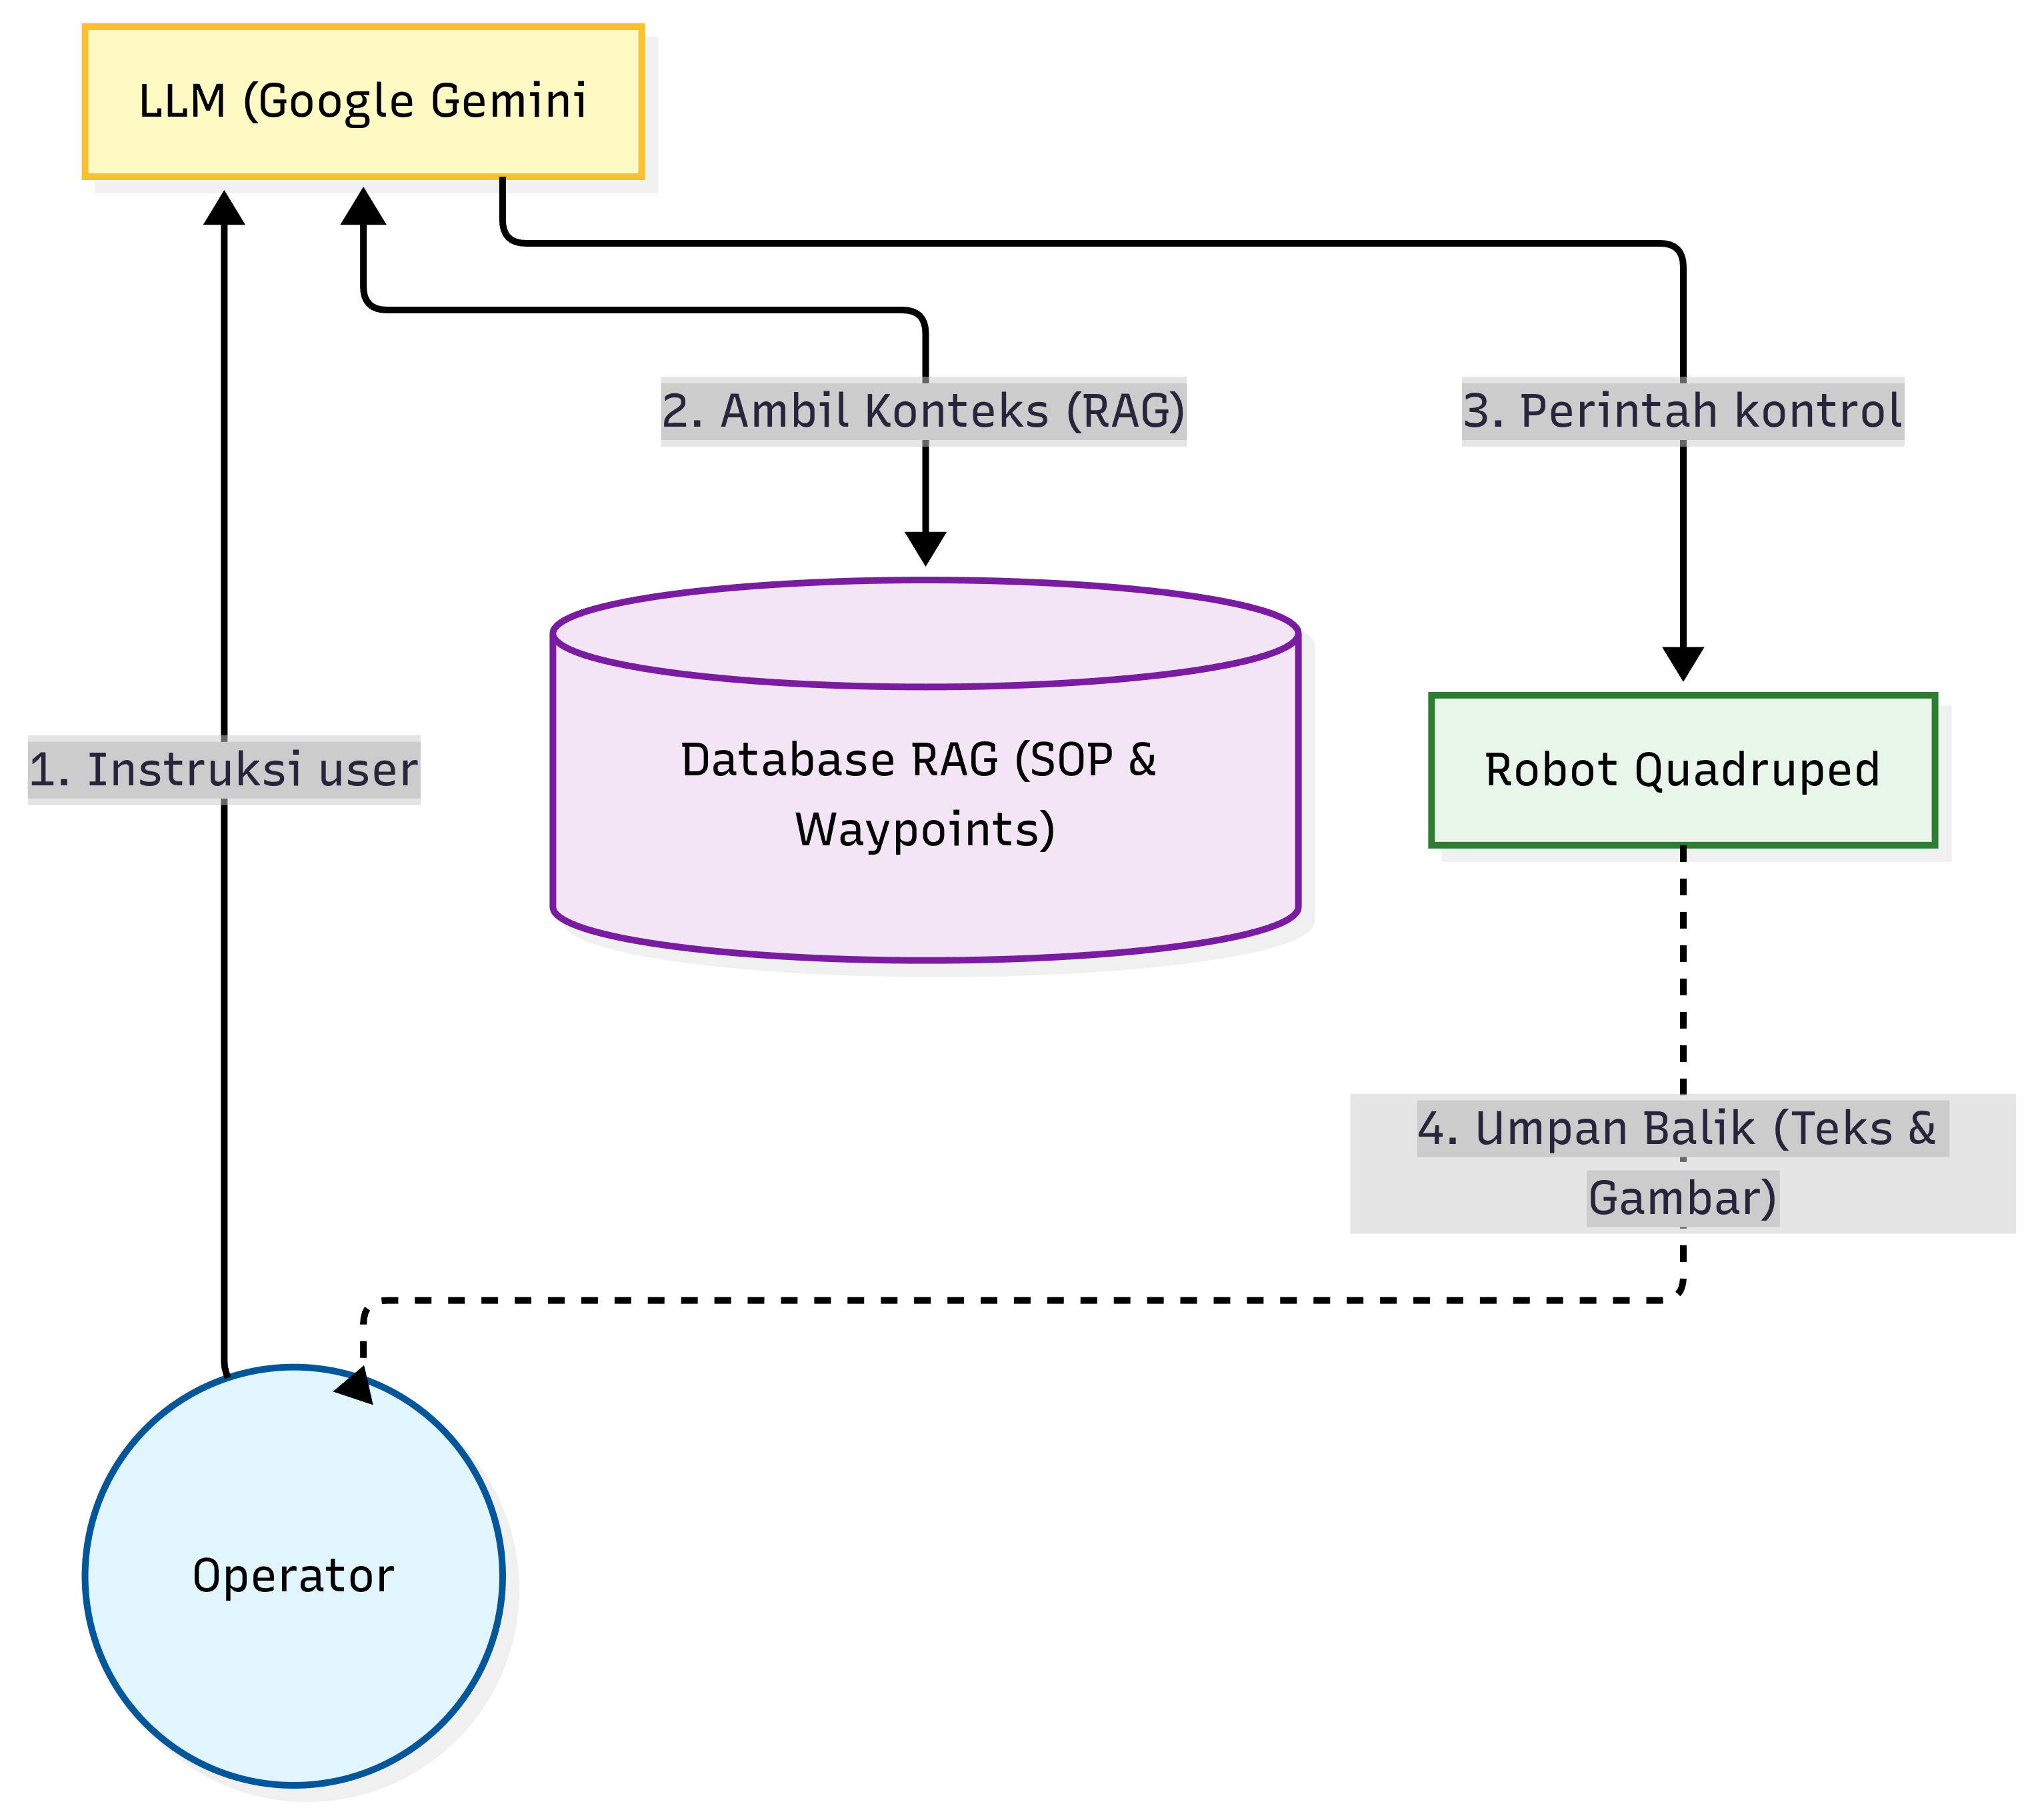
\includegraphics[width=0.5\textwidth]{Init/gambar/umum.png} 
    \caption{Diagram Umum Sistem}
    \label{fig:high_level_diagram}
\footnotesize \textbf{Sumber:} Dokumentasi Penulis
\end{figure}

Mekanisme kerja sistem diawali dengan pemberian instruksi oleh operator menggunakan bahasa alami berupa nama objek target inspeksi. Perintah abstrak ini kemudian diproses oleh MLLM, namun tidak langsung diterjemahkan secara harfiah. MLLM secara aktif melakukan pencarian konteks (\textit{Context Retrieval} dengan pendekatan \textit{Agentic RAG}) ke basis data eksternal melalui pemanggilan \textit{tools} untuk mengambil informasi pendukung yang relevan, seperti peta semantik, titik koordinat \textit{waypoints}, serta dokumen \textit{Standard Operating Procedure} (SOP) yang berkaitan dengan objek inspeksi. Langkah ini krusial untuk memastikan bahwa keputusan yang diambil oleh MLLM didasarkan pada data spasial dan prosedural yang akurat, bukan sekadar halusinasi model bahasa.

Setelah pemahaman kontekstual terbentuk, MLLM tidak secara langsung memerintah robot, melainkan menyusun rencana inspeksi dan mengeksekusinya melalui serangkaian pemanggilan \textit{tools}. Pemanggilan \textit{tools} inilah yang kemudian meneruskan perintah navigasi dan kontrol ke robot \textit{quadruped} untuk dieksekusi, menggerakkan aktuator fisik menuju lokasi target secara otonom. Sistem ini menerapkan mekanisme eksekusi secara bertahap. Setelah menyelesaikan suatu aksi navigasi atau pengambilan data, sistem akan mengirimkan laporan status beserta bukti visual kembali kepada operator. Mekanisme ini memberikan kesempatan bagi operator untuk memvalidasi hasil tindakan robot sebelum sistem diizinkan mengeksekusi \textit{tool} tahap berikutnya, sehingga menjamin keamanan dan adaptabilitas operasi inspeksi di lingkungan yang dinamis.

\subsection{Arsitektur Sistem}
Arsitektur sistem dalam penelitian ini menggunakan pendekatan terdistribusi yang mengintegrasikan kemampuan penalaran tingkat tinggi dari \textit{Multimodal Large Language Model} (MLLM) dengan sistem kendali robotik. Kompo\-nen-kompo\-nen sistem dirancang secara modular dan saling terhubung melalui jaringan TCP/IP lokal maupun internet. Gambaran menyeluruh mengenai arsitektur sistem dan topologi data disajikan pada Gambar \ref{fig:arsitektur_sistem}.

\begin{figure}[H]
    % Pastikan diagram mermaid baru sudah di-export jadi gambar
    \centering
    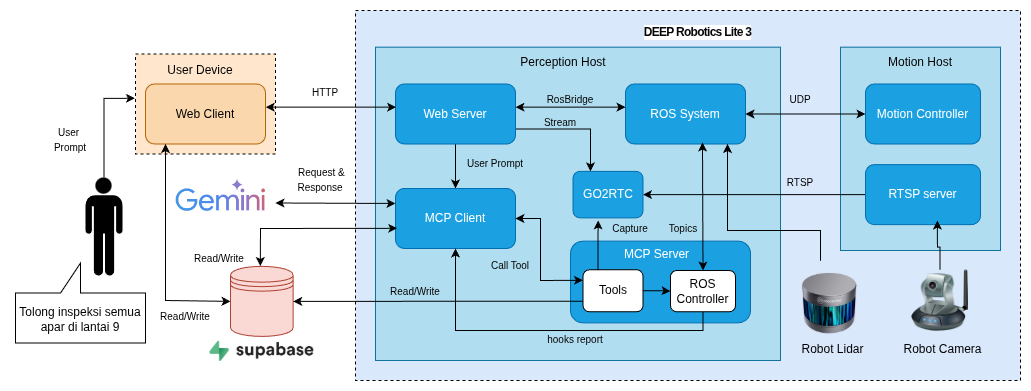
\includegraphics[width=1.0\textwidth]{Init/gambar/arsitektur_new.png}
    \caption{Diagram Arsitektur Sistem}
    \label{fig:arsitektur_sistem}
    \footnotesize \textbf{Sumber:} Dokumentasi Penulis
\end{figure}


\subsubsection{Google Gemini API}
Google Gemini API merupakan komponen yang berperan sebagai otak pemroses utama untuk sistem inspeksi. Pemilihan model Gemini didasarkan pada keunggulannya yang memiliki rasio nilai performa berbanding harga paling baik di antara model \textit{multimodal} lainnya di pasaran, sembari tetap mempertahankan kemampuannya dalam memproses analisis visual secara \textit{zero-shot} tanpa memerlukan pelatihan ulang pada data kustom. Gemini berfungsi untuk memahami perintah bahasa alami dari operator yang dikirim melalui \textit{Web Client}. Perintah tersebut dianalisis untuk membuat rencana inspeksi. Gemini menggunakan fitur \textit{function calling} untuk mengakses berbagai \textit{tools} yang ada pada MCP Server. Dengan fitur ini, Gemini bisa memutuskan kapan harus menggerakkan robot, kapan harus mengambil foto, atau kapan harus mencari dokumen SOP di \textit{database}. Gemini API juga berperan dalam proses analisis visual pada saat inspeksi berlangsung. Ketika kamera robot menangkap \textit{image} sebuah objek, \textit{image} tersebut dikirim ke Gemini API bersamaan dengan instruksi dari dokumen SOP. Gemini akan membandingkan kondisi visual objek pada foto dengan standar yang tertulis di SOP. Detail implementasi dari komponen ini dijelaskan pada Subbab 3.2.2.6.

\subsubsection{Supabase}
Supabase dalam sistem ini diimplementasikan sebagai platform pusat penyimpanan data yang digunakan oleh \textit{Web Client}, \textit{MCP Client}, dan \textit{MCP Server}. Penggunaan platform Supabase pada arsitektur ini didasarkan pada kebutuhan sistem akan penyatuan fungsional antara basis data relasional dan penyimpanan berkas objek di dalam satu ekosistem yang tersinkronisasi. Fungsi pertama dari Supabase adalah sebagai \textit{database} relasional. Di dalam \textit{database} ini, sistem menyimpan daftar lokasi dan koordinat target. Selain itu, \textit{database} juga digunakan untuk menyimpan log \textit{Session History} yang berisi riwayat percakapan antara operator dan Gemini agar konteks memori misi sebelumnya tetap terjaga. Fungsi kedua adalah sebagai \textit{Storage} untuk menyimpan dokumen dan \textit{image}. Komponen penyimpanan ini digunakan secara spesifik untuk menyimpan fail dokumen SOP, serta setiap foto hasil tangkapan kamera robot saat proses inspeksi di lapangan berlangsung. Detail implementasi dari komponen ini dijelaskan pada Subbab 3.2.5.

\subsubsection{\textit{Web App}}
\textit{Web App} merupakan antarmuka utama yang digunakan oleh operator untuk mengendalikan dan memantau robot. \textit{Web App} ini dijalankan di dalam PC internal robot dan difungsikan secara spesifik untuk memfasilitasi peran pengawasan manusia (\textit{Human-in-the-Loop}). Komponen ini bertindak sebagai media komunikasi antara operator dan \textit{AI Agent} melalui panel \textit{chat}. Selain itu, \textit{Web App} juga menyediakan fitur manajemen data untuk mengatur lokasi \textit{waypoint} target dan mengelola dokumen panduan inspeksi. Fungsi lainnya adalah sebagai pusat pemantauan \textit{real-time}, di mana komponen ini mengeksekusi pemuatan aliran video secara langsung dari kamera robot menggunakan protokol WebRTC serta menampilkan data telemetri robot melalui koneksi \textit{Rosbridge WebSocket}. Detail implementasi dari komponen ini dijelaskan pada Subbab 3.2.1.

\subsubsection{MCP \textit{Client}}
MCP \textit{Client} dirancang sebagai perantara komunikasi (\textit{middleware}) antara antarmuka web, Gemini API, dan MCP Server dalam menjalankan mekanisme \textit{Agentic Loop}. Komponen MCP \textit{Client} ini mengeksekusi tiga logika krusial. Pertama, komponen ini mengelola \textit{System Prompt} untuk menginjeksikan konfigurasi kepribadian serta batasan operasional yang harus dipatuhi oleh Gemini sebelum pesan dikirim. Kedua, ketika Gemini menghasilkan balasan berupa pemanggilan alat bantu (\textit{function calling}), komponen ini menerjemahkan pesan perintah tersebut menjadi instruksi berformat HTTP dan meneruskannya ke \textit{tools} yang sesuai pada MCP Server. Ketiga, setelah memperoleh respons balasan dari robot, komponen ini akan mengirimkan kembali hasil tersebut kepada Gemini sekaligus menyinkronkan data interaksi riwayat percakapan ke dalam \textit{database} Supabase. Detail implementasi dari komponen ini dijelaskan pada Subbab 3.2.2.

\subsubsection{MCP \textit{Server}}
MCP Server beroperasi sebagai lapisan abstraksi dieksekusi di dalam robot. Komponen ini bertugas mengekspos seluruh fungsionalitas sistem operasi robot (ROS) menjadi kumpulan \textit{tools} sederhana yang siap dipanggil oleh agen AI dari luar. Komponen server ini, bertugas mendengarkan perintah pemanggilan \textit{tools} dari agen AI melalui MCP Client, lalu mengeksekusinya. \textit{Tools} ini mencakup pengiriman instruksi bergerak menggunakan fungsionalitas ROS, penangkapan \textit{image} dari kamera robot, pencarian koordinat \textit{waypoint} dan dokumen SOP dari basis data, hingga pelaksanaan komputasi analisis \textit{image}. Selain itu, komponen MCP Server juga mengeksekusi mekanisme \textit{webhook} untuk mengirimkan status ke MCP \textit{Client} setelah aksi pergerakan robot selesai. Detail implementasi dari komponen ini dijelaskan pada Subbab 3.2.3.

\subsubsection{Sistem ROS}
ROS berperan sebagai sistem yang mengelola seluruh komunikasi dan tugas navigasi pada robot. Di dalam komponen ROS ini, terdapat \textit{node} spesifik yang beroperasi, di antaranya adalah \textit{Navigation Stack} yang memproses data mentah lidar untuk menghasilkan peta lingkungan serta mengeksekusi perencanaan jalur (\textit{path planning}) selama misi berlangsung. Seluruh koordinasi pergerakan fisik dikelola melalui koneksi UDP menuju \textit{Motion Host}. Untuk menjembatani komunikasi dengan antarmuka luar, \textit{RosBridge Server} digunakan untuk mengeksekusi pembukaan protokol \textit{WebSocket} yang memungkinkan \textit{Web App} mengakses data telemetri robot. Integrasi antara ekosistem ROS dengan MCP Server dilakukan melalui mekanisme \textit{topics} yang memungkinkan \textit{tools} pada server mengakses fungsionalitas pergerakan robot. Detail implementasi dari komponen ini dijelaskan pada Subbab 3.2.4.

\subsubsection{\textit{Motion Controller}}
\textit{Motion Controller} merupakan unit kendali fisik tingkat terendah (\textit{low-level}) bawaan yang tertanam dan berinteraksi langsung dengan perangkat keras robot Jueying Lite3. Komponen ini ditempatkan di posisi paling ujung dalam rantai perintah pergerakan. Di dalam subsistem ini, dieksekusi proses komputasi yang memegang kendali atas keseimbangan dinamis mekanik dan rotasi sendi-sendi aktuator kaki (\textit{gait planning}). Komponen ini bertugas menerima perintah vektor abstraksi kecepatan (\textit{velocity command}) dari ekosistem ROS, lalu mengeksekusi penerjemahannya menjadi sinyal daya putaran torsi motor yang secara aktual menggerakkan fisik robot. Detail implementasi dari komponen ini dijelaskan pada Subbab 3.2.4.4.

\subsubsection{GO2RTC}
 Komponen GO2RTC digunakan untuk mengelola distribusi aliran data visual dari kamera robot menuju berbagai modul dalam sistem. Komponen ini menerima aliran data bervolume tinggi melalui protokol RTSP dari \textit{RTSP server} yang terhubung langsung dengan perangkat keras kamera pada \textit{Motion Host}. GO2RTC kemudian mengeksekusi konversi aliran protokol transmisi tersebut menjadi format WebRTC agar dapat diakses dengan latensi sekecil mungkin oleh modul \textit{Web App} dan MCP Server. Detail implementasi dari komponen ini dijelaskan pada Subbab 3.2.1.1 dan Subbab 3.2.3.7.

\subsubsection{RTSP \textit{Server}}
RTSP \textit{server} beroperasi di dalam modul \textit{Motion Host} sebagai penyedia akses data visual mentah yang bersumber langsung dari kamera robot. Di dalam siklus kerjanya, komponen ini memiliki tanggung jawab untuk mengeksekusi pengambilan data \textit{image}, mengelola aliran data video tersebut, dan menyediakannya dalam format transmisi standar melalui protokol \textit{Real-Time Streaming Protocol} agar dapat dikonsumsi oleh komponen distribusi lanjutan seperti GO2RTC. Detail implementasi dari komponen ini dijelaskan pada Subbab 3.2.1.1 dan Subbab 3.2.3.7.

\subsection{Alur Sistem}

Alur kerja dari sistem inspeksi visual otonom ini dibagi menjadi tiga fase utama, yaitu fase perencanaan, fase eksekusi dan analisis, serta fase pelaporan hasil. Interaksi data dan pesan antarkomponen untuk menyelesaikan sebuah misi divisualisasikan melalui diagram sekuensial pada Gambar \ref{fig:sequence_diagram}. 

\begin{figure}[H]
    \centering
    \includegraphics[width=0.8\textwidth]{Init/gambar/alur_baru.png}
    \caption{Diagram Sekuensial Alur Interaksi Sistem}
    \label{fig:sequence_diagram}
\footnotesize \textbf{Sumber:} Dokumentasi Penulis
\end{figure}

Diagram sekuensial pada Gambar \ref{fig:sequence_diagram} merepresentasikan lima aktor utama (ditunjukkan oleh kotak di bagian atas) yang berpartisipasi dalam siklus sistem, yaitu: Operator manusia, Agen AI (bertindak sebagai MCP \textit{Client}), MCP \textit{Server}, Supabase (sebagai pusat basis data), dan fisik robot \textit{quadruped} (menjalankan ROS dan kamera). Garis lurus tebal (\textit{solid line}) yang mengarah dari satu aktor ke aktor lain menggambarkan pengiriman perintah atau permintaan (\textit{request}), sedangkan garis putus-putus (\textit{dashed line}) menggambarkan pengembalian data atau respons (\textit{callback/return}). Kotak vertikal panjang yang berada di bawah setiap aktor merepresentasikan waktu aktif (\textit{lifeline}) di mana komponen tersebut sedang memproses suatu tugas. Seluruh komponen ini bekerja secara sinkron dan saling melengkapi melalui tiga fase utama berikut.

\subsubsection{Fase Perencanaan}

Fase perencanaan berfokus pada penerimaan instruksi abstrak dari manusia dan penyusunan rencana kerja terstruktur oleh sistem sebelum robot melakukan pergerakan fisik. Seperti yang diilustrasikan pada sepertiga awal diagram, proses interaksi pesan pada fase ini diuraikan sebagai berikut:

\begin{enumerate}
    \item \textbf{\textit{User Prompt}:} Operator memasukkan perintah bahasa alami melalui panel obrolan (\textit{chat}) pada antarmuka web, yang langsung diteruskan kepada agen AI (gabungan MCP \textit{Client} dan Gemini).
    \item \textbf{\textit{Execute Tool} Pencarian:} Merespons instruksi tersebut, agen AI mengirimkan perintah ke MCP Server untuk mengeksekusi \textit{tool} pencarian data koordinat objek (\textit{waypoint}) dan dokumen SOP.
    \item \textbf{\textit{Query Data}:} MCP Server meneruskan perintah tersebut dengan melakukan kueri ke basis data Supabase.
    \item \textbf{\textit{Return Coordinates \& SOP Content}:} Supabase merespons dengan mengembalikan data titik koordinat spasial beserta isi panduan inspeksi secara terstruktur.
    \item \textbf{\textit{Tool Result}:} MCP Server meneruskan data hasil pencarian tersebut kembali kepada agen AI sebagai konteks misi.
    \item \textbf{\textit{Plan Result}:} Agen AI memproses seluruh data konteks, menghasilkan draf rencana inspeksi secara utuh, dan menampilkannya kembali ke layar antarmuka Operator untuk ditinjau.
    \item \textbf{\textit{User Confirmation}:} Di titik pengawasan ini, Operator memberikan persetujuan eksplisit untuk mengesahkan rencana kerja sebelum robot diberi izin untuk mulai bergerak.
\end{enumerate}

\subsubsection{Fase Eksekusi dan Analisis}

Fase kedua merupakan tahap di mana sistem mulai menggerakkan perangkat keras robot dan melakukan pemrosesan visual berdasarkan rencana yang telah disetujui. Langkah-langkah interaksi pada fase ini adalah sebagai berikut:

\begin{enumerate}
    \setcounter{enumi}{7}
    \item \textbf{\textit{Execute Tool Navigation}:} Setelah konfirmasi dari operator, agen AI mengirimkan perintah ke MCP Server untuk mengeksekusi \textit{tool} navigasi pergerakan fisik.
    \item \textbf{\textit{Send ROS Messages}:} MCP Server menerjemahkan perintah abstrak tersebut dengan menembakkan pesan instruksi teknis ke dalam sistem ROS pada robot agar mulai bergerak secara otonom.
    \item \textbf{\textit{Status Running}:} Segera setelah perintah pergerakan terkirim, MCP Server membalas agen AI dengan status "running" agar siklus AI tidak membeku sembari menunggu perjalanan yang memakan waktu.
    \item \textbf{\textit{Status Arrived}:} Saat robot mencapai titik koordinat spasial yang dituju, sistem ROS mendeteksi keberhasilan navigasi dan mengirimkan status kedatangan ke MCP Server.
    \item \textbf{\textit{Webhook Report}:} MCP Server meneruskan status kedatangan tersebut dengan mekanisme \textit{webhook} kepada agen AI untuk memicu \textit{agent loop} kembali.
    \item \textbf{\textit{Execute Tool Capture}:} Agen AI langsung mengirimkan perintah lanjutan kepada MCP Server untuk mengeksekusi pengambilan \textit{image}.
    \item \textbf{\textit{Capture Image}:} MCP Server menjalankan perintah pengambilan \textit{image} ini dengan cara mengakses kamera melalui GO2RTC.
    \item \textbf{\textit{Image Result}:} GO2RTC pada robot merespons dengan mengembalikan biner \textit{image} secara utuh kembali kepada MCP Server.
    \item \textbf{\textit{Save Image}:} MCP Server mengirimkan \textit{image} tersebut ke basis data Supabase untuk diarsipkan ke dalam \textit{Storage}.
    \item \textbf{\textit{Image URL \& Analysis Result}:} Bersamaan dengan itu, MCP Server melampirkan tautan URL \textit{image} serta mengembalikan hasil analisis \textit{image} kembali kepada agen AI agar dapat difinalisasi.
\end{enumerate}

\subsubsection{Fase Pelaporan}

Fase pelaporan merupakan tahap penutup dari satu siklus inspeksi objek tunggal, di mana hasil kerja robot dilaporkan dan keputusan kelanjutan misi dikembalikan ke tangan manusia. Rincian percabangan pesannya adalah sebagai berikut:

\begin{enumerate}
    \setcounter{enumi}{17}
    \item \textbf{\textit{Show Analysis Result}:} Agen AI menyajikan narasi evaluasi akhir kondisi objek beserta bukti visual \textit{image} ke layar antarmuka obrolan agar dapat diperiksa langsung oleh Operator.
    \item \textbf{\textit{Interruption Prompt} (Skenario Intervensi):} Apabila Operator mendeteksi adanya kejanggalan pada foto visual yang ditayangkan, alur masuk ke percabangan di mana operator segera mengetikkan instruksi interupsi manual (misal: "Maju sedikit, foto lagi").
    \item \textbf{\textit{Execute Tools} (Skenario Intervensi):} Merespons interupsi, agen AI memberikan perintah eksekusi \textit{tool} sesuai instruksi interupsi operator melalui MCP Server.
    \item \textbf{\textit{User Confirmation} (Skenario Lanjut):} Sebaliknya pada jalur alternatif kedua, apabila Operator merasa puas dengan hasil analisis objek tersebut, ia memberikan izin persetujuan kepada AI untuk meneruskan sisa misinya.
    \item \textbf{\textit{Go To Next Waypoint} (Skenario Lanjut):} Setelah menerima izin kelanjutan, agen AI akan kembali mengeksekusi instruksi pergerakan ke titik lokasi target berikutnya. Seluruh siklus komunikasi dari nomor tujuh akan terus berulang hingga seluruh rangkaian rencana inspeksi terselesaikan.
\end{enumerate}

\subsection{Mekanisme (\textit{Human-in-the-Loop})}

Dalam arsitektur sistem ini, mekanisme \textit{Human-in-the-Loop} (HITL) diimplementasikan melalui panel obrolan (\textit{chat}) pada antarmuka web, di mana operator bertindak sebagai supervisor yang mengawasi dan menyetujui setiap keputusan agen AI. Agen AI diprogram melalui \textit{system prompt} untuk tidak mengeksekusi aksi robot atau memodifikasi rencana tanpa persetujuan eksplisit dari operator. Pendekatan ini tidak hanya meminimalisasi risiko kecelakaan atau kerusakan lingkungan akibat salah tafsir perintah, tetapi juga memberikan fleksibilitas tinggi bagi operator untuk menyesuaikan misi di lapangan.

Berdasarkan perancangan sistem, terdapat empat skenario utama kasus intervensi operator yang akan diuji untuk memvalidasi kapabilitas sistem:

\begin{enumerate}
    \item \textbf{Intervensi Perubahan Rencana Awal:} 
    Operator meminta perubahan rencana sesaat setelah agen AI menyusun \textit{inspection plan} namun sebelum robot bergerak. Contoh kasus: setelah sistem merencanakan inspeksi, operator mengintervensi dengan meminta agen untuk menambahkan instruksi agar robot mengambil posisi duduk setelah seluruh misi selesai.
    
    \item \textbf{Intervensi Penambahan Rencana di Tengah Misi:} 
    Operator memberikan instruksi baru saat robot sudah menjalankan sebagian misi. Contoh kasus: ketika robot baru saja selesai menginspeksi stop kontak dan bersiap ke tujuan berikutnya, operator meminta penambahan objek inspeksi baru (seperti tong sampah) ke dalam antrean rencana.
    
    \item \textbf{Intervensi Pembatalan Objek:} 
    Operator mengubah pikiran dengan membatalkan target inspeksi tertentu dan menggantinya dengan target lain. Contoh kasus: saat agen merencanakan inspeksi ke beberapa objek, operator menginstruksikan untuk membatalkan pemeriksaan pada satu stop kontak dan menukar beban tugasnya dengan menambah inspeksi pada satu tong sampah ekstra.
    
    \item \textbf{Intervensi Manuver:} 
    Operator memberikan intervensi untuk mengontrol pergerakan robot demi mendapatkan sudut pandang visual yang lebih baik ketika mendeteksi anomali. Contoh kasus: saat robot tiba di depan sebuah APAR yang kondisinya terlihat mencurigakan, operator menyuruh robot untuk "maju mendekat sedikit" sebelum memicu pengambilan \textit{image} ulang, guna memverifikasi kondisi objek dengan lebih jelas.
\end{enumerate}

Skenario-skenario intervensi ini merepresentasikan kondisi operasional dunia nyata yang dinamis, di mana sistem AI tidak boleh berjalan secara buta melainkan harus mampu beradaptasi dengan instruksi diskresi dari supervisor manusianya.

\subsection{Desain \textit{Web App}}

Desain antarmuka \textit{Web App} dirancang menggunakan pendekatan tata letak fungsional yang berfokus pada kemudahan \textit{monitoring} dan intervensi operator. Pembuatan rancangan awal (\textit{wireframe}) dari aplikasi web ini memuat beberapa halaman utama yang mendukung alur kerja inspeksi.

\subsubsection{Halaman Inspeksi}
\begin{figure}[H]
    \centering
    
\includegraphics[width=0.8\textwidth]{Init/gambar/wireframe/inspection_hub.png}
    \caption{Desain Antarmuka Halaman Inspeksi}
    \label{fig:desain_inspection_hub}
\footnotesize \textbf{Sumber:} Dokumentasi Penulis
\end{figure}
Halaman Inspeksi merupakan rancangan antarmuka utama di mana operator berinteraksi dengan sistem. Pada desain ini, tata letak dibagi menjadi panel percakapan di sisi kiri untuk berkomunikasi dengan agen AI, serta panel pemantauan di sisi kanan yang menayangkan aliran video secara langsung dari kamera robot dan representasi peta navigasi spasial. Selanjutnya, terdapat bar pada bagian atas untuk data telemetri robot.

\subsubsection{Halaman Manajemen Lokasi dan \textit{Waypoint}}
\begin{figure}[H]
    \centering
    
\includegraphics[width=0.8\textwidth]{Init/gambar/wireframe/spatial_explorer.png}
    \caption{Desain Antarmuka Halaman Manajemen Lokasi dan \textit{Waypoint}}
    \label{fig:desain_spatial_explorer}
\footnotesize \textbf{Sumber:} Dokumentasi Penulis
\end{figure}
Desain Halaman Manajemen Lokasi dan \textit{Waypoint} difokuskan untuk mempermudah operator dalam mengatur struktur data spasial. Antarmuka ini menampilkan hierarki lokasi dan tabel daftar koordinat target (\textit{waypoint}) yang memungkinkan operator untuk menambah, mengubah, atau menghapus titik tujuan inspeksi di dalam basis data.

\subsubsection{Halaman Manajemen SOP}
\begin{figure}[H]
    \centering
    
\includegraphics[width=0.8\textwidth]{Init/gambar/wireframe/sop.png}
    \caption{Desain Antarmuka Halaman Manajemen SOP}
    \label{fig:desain_sop_manager}
\footnotesize \textbf{Sumber:} Dokumentasi Penulis
\end{figure}
Rancangan Halaman Manajemen SOP bertujuan untuk memfasilitasi pengelolaan dokumen SOP inspeksi. Antarmuka ini menyediakan area khusus bagi pengguna untuk mengunggah berkas SOP secara langsung dengan mekanisme \textit{drag-and-drop} dan menampilkan daftar dokumen yang tersimpan dalam format \textit{grid} kartu untuk mempermudah pencarian.

\subsubsection{Halaman Riwayat Inspeksi}
\begin{figure}[H]
    \centering
    
\includegraphics[width=0.8\textwidth]{Init/gambar/wireframe/history.png}
    \caption{Desain Antarmuka Halaman Riwayat Inspeksi}
    \label{fig:desain_history_log}
\footnotesize \textbf{Sumber:} Dokumentasi Penulis
\end{figure}
Halaman Riwayat Inspeksi dirancang untuk menyajikan daftar seluruh sesi misi yang pernah dieksekusi. Desain antarmuka memuat tabel log sesi yang dilengkapi dengan fitur \textit{sliding panel}, sehingga operator dapat meninjau ulang isi percakapan dan analisis AI pada sesi terdahulu secara utuh.

\subsubsection{Halaman Galeri \textit{Image}}
\begin{figure}[H]
    \centering
    
\includegraphics[width=0.8\textwidth]{Init/gambar/wireframe/captured_gallery.png}
    \caption{Desain Antarmuka Halaman Galeri Tangkapan \textit{Image}}
    \label{fig:desain_image_gallery}
\footnotesize \textbf{Sumber:} Dokumentasi Penulis
\end{figure}
Desain Halaman Galeri \textit{Image} berfokus pada penyajian dokumentasi visual hasil inspeksi yang telah dilakukan sebelumnya. Tata letaknya menggunakan model \textit{grid} di mana setiap foto dari robot ditampilkan sebagai \textit{thumbnail} berserta informasi data penanda waktu pengambilan, dan dapat diperbesar untuk peninjauan lebih detail.

\subsubsection{Halaman Manajemen Objek}
\begin{figure}[H]
    \centering
    
\includegraphics[width=0.8\textwidth]{Init/gambar/wireframe/objects.png}
    \caption{Desain Antarmuka Halaman Manajemen Objek}
    \label{fig:desain_objects}
\footnotesize \textbf{Sumber:} Dokumentasi Penulis
\end{figure}
Halaman Manajemen Objek dirancang untuk mendefinisikan jenis objek yang akan diinspeksi. Antarmuka ini menampilkan tabel daftar nama objek beserta relasinya dengan pedoman SOP yang relevan dan kata kunci, guna membantu agen AI dalam mencari objek dan menyocokkan kondisi visual target dengan standar operasional.

\section{Implementasi Sistem}

Bagian ini membahas penerapan dari desain yang telah diuraikan sebelumnya. Implementasi sistem mencakup pengembangan antarmuka \textit{Web App} untuk operator, pembuatan modul MCP \textit{Client} sebagai jembatan komputasi agen AI, hingga integrasi pada MCP \textit{Server} yang secara fisik mengontrol pergerakan perangkat keras robot. Masing-masing realisasi modul perangkat lunak ini akan dijabarkan secara rinci pada subbab berikut.

\subsection{\textit{Web App}}

Antarmuka Web App dibangun menggunakan kerangka kerja Next.js dengan bahasa pemrograman TypeScript, dan dirancang sebagai \textit{Single Page Application} dengan sistem navigasi halaman internal yang dikelola melalui \textit{state manager}. Pengelolaan dan sinkronisasi data dari basis data Supabase maupun peladen FastAPI ditangani secara terpusat menggunakan pustaka TanStack React Query. Untuk kebutuhan pengontrolan robot, interaksi \textit{real-time} disalurkan melalui pustaka roslibjs yang terhubung langsung ke \textit{Rosbridge WebSocket} pada sistem robot. Aliran video dari kamera robot juga dirender secara langsung melalui protokol WebRTC yang bersumber dari komponen GO2RTC. Sementara itu, rancangan antarmuka dikonfigurasi menggunakan utilitas Tailwind CSS dan didukung oleh library GSAP untuk memberikan umpan balik animasi visual kepada operator.

\subsubsection{Halaman Inspeksi}
\begin{figure}[h!]
    \centering
    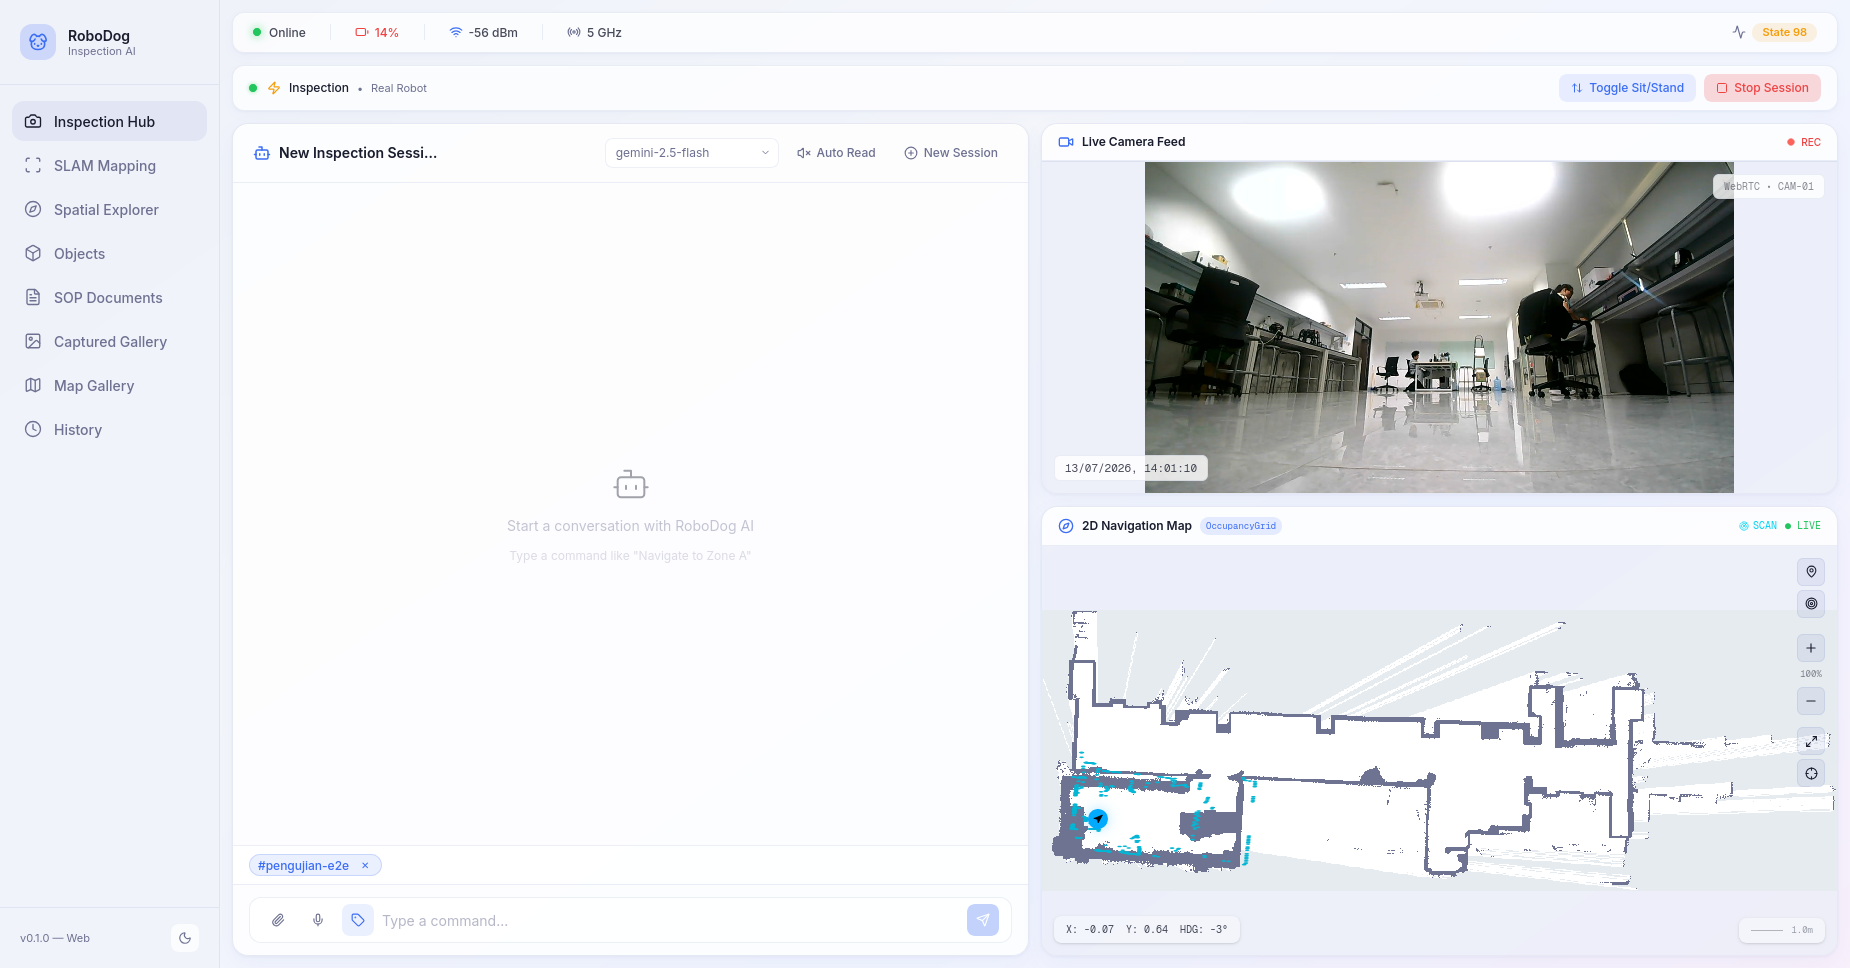
\includegraphics[width=0.8\textwidth]{Init/gambar/web_img/inspection_hub.png}
    \caption{Tampilan Halaman Inspeksi}
    \label{fig:inspection_hub}
\footnotesize \textbf{Sumber:} Dokumentasi Penulis
\end{figure}
Seperti yang ditampilkan pada Gambar \ref{fig:inspection_hub}, Halaman Inspeksi merupakan antarmuka utama bagi operator untuk mengendalikan misi robot secara interaktif. Sebelum memasuki antarmuka utama ini, operator disajikan dengan tombol untuk memulai peluncuran. Proses inisialisasi ini dipicu dengan mengeksekusi skrip inisialisasi navigasi robot quadruped berupa berkas bash melalui Next.js API route /api/shell di sisi server. Ketika sesi inisialisasi aktif dan terhubung, halaman akan memuat tata letak grid dinamis yang menggabungkan panel chat di sisi kiri serta panel video feed dan peta navigasi di sisi kanan.

Panel chat tersebut terhubung dengan Gemini API dan menyediakan menu pilihan model bahasa gemini seperti gemini-2.5-flash, gemini-3.1-pro-\allowbreak preview, gemini-3-flash-\allowbreak preview, gemini-3.1-flash-lite, dan gemini-2.5-pro. Setiap pesan operator secara otomatis menyertakan data telemetri robot real-time dari WebSocket Rosbridge. Data baterai diambil dari topic /battery\_\allowbreak level dengan tipe pesan std\_msgs/\allowbreak Float64, status gerakan dari topic /robot\_\allowbreak basic\_\allowbreak state dengan tipe pesan std\_msgs/\allowbreak Int32, dan koordinat posisi dari topic /odom dengan tipe pesan nav\_msgs/\allowbreak Odometry. Seluruh telemetri ini ditambahkan ke dalam pesan pengguna sebagai metadata status agar model bahasa memiliki pemahaman konteks fisik aktual robot.

Saat operator menekan tombol kirim pesan, chat request akan melakukan hit pada Next.js API route /api/chat yang kemudian meneruskan data tersebut untuk memanggil endpoint API pada MCP client. Untuk menampilkan percakapan secara dinamis, Web App melakukan subscribe ke database Supabase secara real-time menggunakan Supabase Realtime channel subscription pada tabel chat-\allowbreak messages yang difilter berdasarkan ID sesi aktif. Hal ini memungkinkan setiap pembaruan pesan baru, termasuk respons teks dan log pemanggilan tool dari MCP client, langsung dirender di antarmuka pengguna secara instan tanpa memuat ulang halaman.

Mekanisme render chat memilah peran pesan antara user dan assistant yang tersimpan dalam kolom content bertipe JSONB di tabel database. Sistem menyembunyikan log pemanggilan fungsi internal untuk menyajikan percakapan yang bersih kepada operator. Namun, apabila terdapat respon fungsi dari tool inspeksi \textit{image}, sistem secara dinamis mendeteksi URL \textit{image} publik dari bucket storage pada folder captured dan merendernya dalam bentuk komponen \textit{image} di panel obrolan. Pesan teks biasa dirender dengan pemformatan Markdown dasar seperti cetak tebal, cetak miring, dan inline code.

Di bagian atas panel terdapat \textit{active session bar} yang menyediakan tombol kontrol gerakan fisik berupa \textit{Toggle Sit/Stand} untuk menerbitkan perintah perubahan postur tubuh robot ke topic /simple\_cmd dengan tipe pesan message\_transformer/SimpleCMD menggunakan kode perintah 0x21010202. Di sebelah tombol tersebut, terdapat tombol \textit{Stop Session} yang digunakan untuk menghentikan program navigasi robot secara penuh. Ketika tombol ini ditekan, Web App akan memanggil Next.js API route /api/shell untuk menjalankan skrip pemutus proses berupa berkas bash stop\_nav.sh, menghentikan pengiriman heartbeat periodik 0x21040001 sebesar dua hertz untuk mencegah robot masuk ke mode proteksi kehilangan kontrol, memutus koneksi WebSocket Rosbridge, dan mengembalikan tampilan ke halaman inisialisasi awal.

Pada sudut kanan atas panel chat, operator dapat menggunakan tombol \textit{New Session} untuk memulai percakapan baru. Mekanisme ini bekerja dengan mengosongkan ID sesi aktif di state manager menjadi bernilai null dan membersihkan cache pesan sesi sebelumnya pada React Query. Judul sesi baru akan dibuat secara otomatis pada database Supabase di tabel chat-sessions sesaat setelah operator mengirimkan pesan pertama kali, dengan format penamaan default Session diikuti dengan nomor ID unik sesi tersebut.

Panel video feed di sisi kanan atas menampilkan stream kamera secara real-time dari go2rtc menggunakan protokol WebRTC yang dibungkus dalam elemen iframe. Tepat di bawah panel video, terdapat peta navigasi dua dimensi yang memproses data peta OccupancyGrid dari topic /map secara real-time. Peta ini mendeteksi pesan ROS dan mengonversinya menjadi \textit{image} menggunakan elemen canvas dengan melakukan rotasi sumbu koordinat agar orientasinya sesuai dengan arah utara robot. Peta navigasi juga menampilkan overlay posisi robot menggunakan data odometry dari topic /odom, data pemindaian laser LiDAR dari topic /scan berupa titik-titik, serta visualisasi jalur navigasi global dari topic /move\_base/\allowbreak Global\-Planner/\allowbreak plan berupa garis putus-putus berwarna kuning. Operator dapat memberikan perintah estimasi posisi awal ke topic /initialpose dengan tipe pesan geometry\_msgs/\allowbreak Pose\-With\-Co\-va\-riance\-Stamped dan target navigasi ke topic /move\_base\_simple/\allowbreak goal dengan tipe pesan geometry\_msgs/\allowbreak Pose\-Stamped secara visual dengan menekan tombol kontrol dan melakukan drag kursor di atas peta.

\subsubsection{Halaman Manajemen Lokasi dan \textit{Waypoint}}
\begin{figure}[h!]
    \centering
    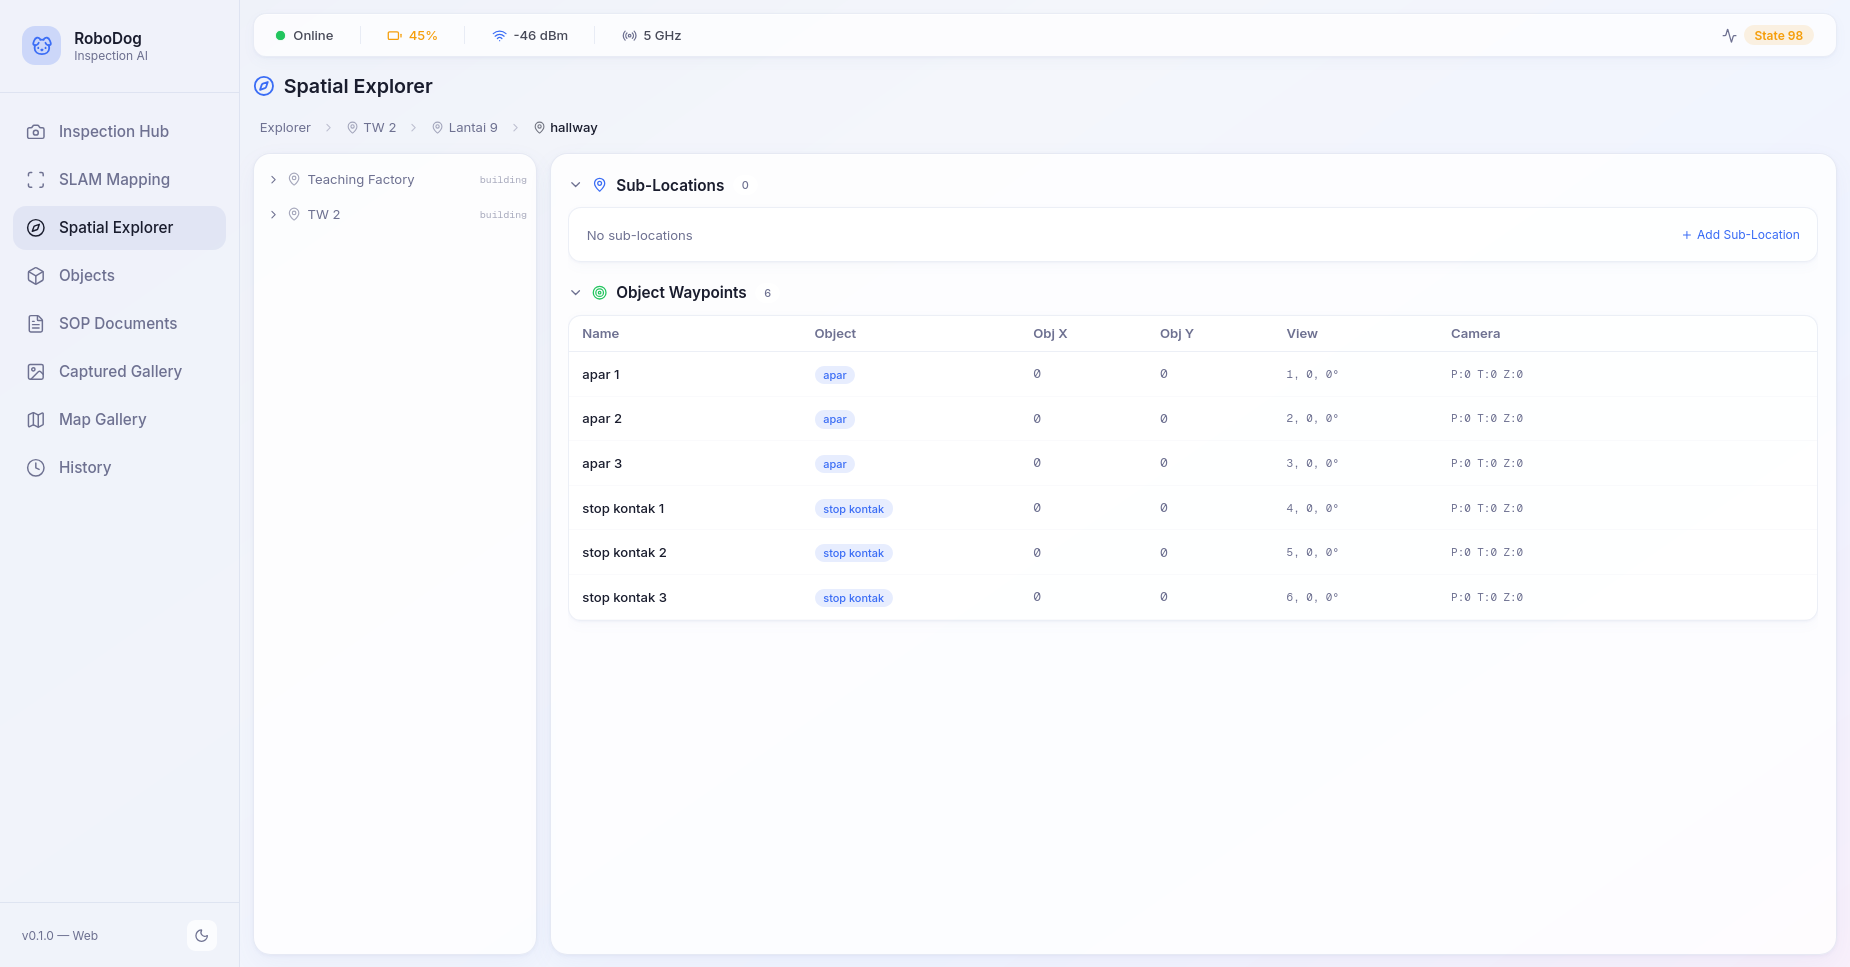
\includegraphics[width=0.8\textwidth]{Init/gambar/web_img/spatial_explorer.png}
    \caption{Tampilan Halaman Manajemen Lokasi dan Waypoint}
    \label{fig:spatial_explorer}
\footnotesize \textbf{Sumber:} Dokumentasi Penulis
\end{figure}
Seperti yang terlihat pada Gambar \ref{fig:spatial_explorer}, Halaman Manajemen Lokasi dan Waypoint atau Spatial Explorer berfungsi untuk mengelola data spasial lingkungan tempat robot beroperasi secara hierarkis. Antarmuka halaman ini terbagi menjadi panel \textit{tree view} di sisi kiri dan tabel daftar data di sisi kanan, dilengkapi dengan baris \textit{breadcrumb} di bagian atas untuk mempermudah pelacakan tingkat lokasi. Hierarki data spasial ini didefinisikan menggunakan beberapa tabel relasional di dalam database Supabase, yaitu tabel maps, locations, sub\_locations, dan object\_waypoints. Peta utama disimpan pada tabel maps, lokasi utama seperti lantai gedung disimpan pada tabel locations, sub-lokasi berupa ruangan disimpan pada tabel sub\_\allowbreak lo\-ca\-tions , dan titik koordinat objek target inspeksi disimpan pada tabel object\_waypoints.

Pada tingkat lokasi utama, halaman ini menyediakan opsi pengaturan koordinat kedatangan robot (meliputi posisi koordinat x, y, dan \textit{yaw}) yang bersifat opsional untuk memosisikan awal robot jika ingin menuju lokasi tersebut. Untuk detail setiap objek target inspeksi pada tabel object\_waypoints, sistem membedakan antara atribut data yang wajib dan opsional. Parameter yang diwajibkan untuk diisi oleh operator hanyalah koordinat pandang robot, yaitu posisi koordinat x, koordinat y, dan sudut \textit{yaw} yang menentukan titik berdiri robot menghadap target saat melakukan inspeksi. Sebaliknya, parameter koordinat fisik asli dari letak objek itu sendiri bersifat opsional. Selain itu, operator juga dapat mendefinisikan konfigurasi kamera berupa sudut \textit{pan}, \textit{tilt}, dan nilai \textit{zoom}. Parameter \textit{Pan-Tilt-Zoom} (PTZ) ini bersifat opsional dan disediakan sebagai bentuk skalabilitas sistem, mengingat kamera bawaan pada robot Jueying Lite3 yang digunakan dalam implementasi ini secara fisik belum mendukung kapabilitas pergerakan mekanis tersebut. Seluruh data konfigurasi spasial ini disimpan secara terpusat di database Supabase dan dapat dikelola secara dinamis oleh operator melalui aksi penambahan, pengubahan, dan penghapusan data yang diimplementasikan menggunakan \textit{form modal}.

\subsubsection{Halaman Manajemen SOP}
\begin{figure}[h!]
    \centering
    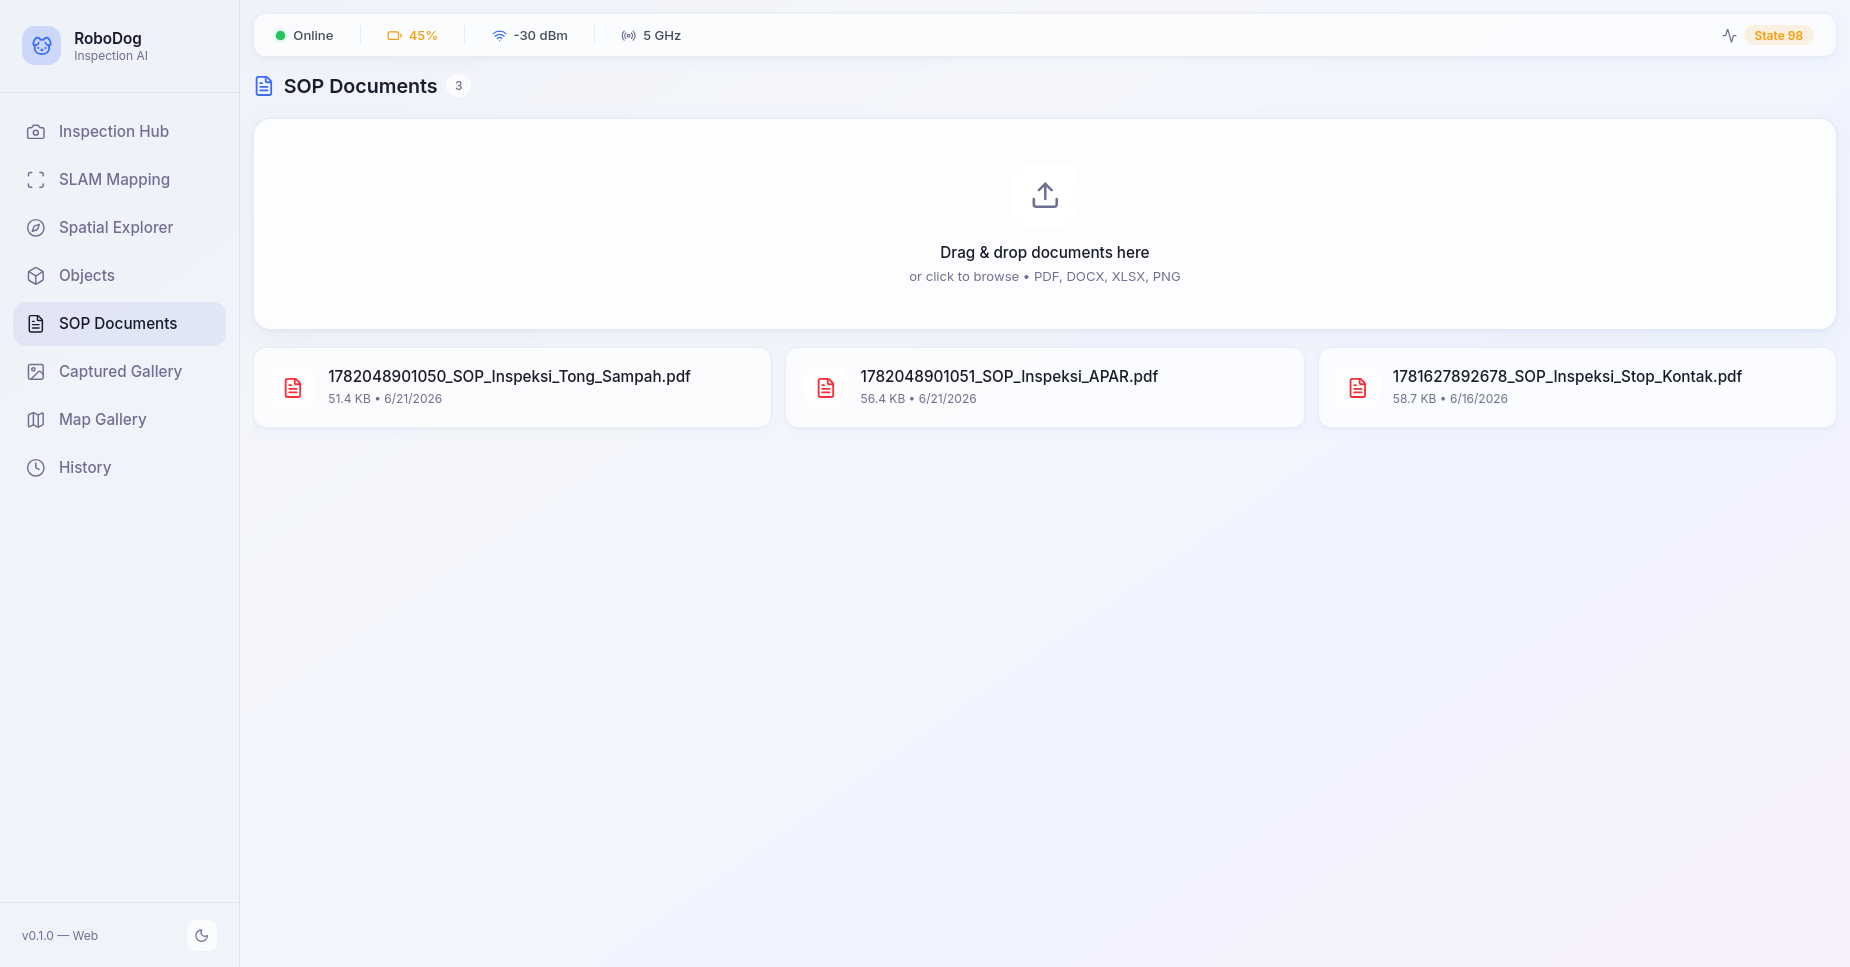
\includegraphics[width=0.8\textwidth]{Init/gambar/web_img/sop.png}
    \caption{Tampilan Halaman Manajemen SOP}
    \label{fig:sop_manager}
\footnotesize \textbf{Sumber:} Dokumentasi Penulis
\end{figure}
Seperti yang terlihat pada Gambar \ref{fig:sop_manager}, Halaman Manajemen SOP digunakan oleh operator untuk mengelola dokumen Standard Operating Procedure yang disimpan di bucket storage pada folder sop pada Supabase. Dokumen SOP ini menjadi acuan bagi agen AI dalam menganalisis kelayakan objek inspeksi. Halaman ini menyediakan area unggah dokumen interaktif yang mendukung fitur \textit{drag} and \textit{drop} berkas langsung dari komputer pengguna. Sistem membatasi jenis berkas yang dapat diunggah seperti dokumen PDF, berkas Word, lembar kerja Excel, atau \textit{image} PNG. Proses pengunggahan dilakukan secara langsung dari browser ke bucket storage Supabase menggunakan SDK client.

Dokumen yang telah berhasil diunggah akan disimpan dengan nama berkas unik yang ditambahkan prefiks penanda waktu timestamp untuk mencegah bentrokan nama berkas. File-file tersebut ditampilkan dalam bentuk grid kartu. Setiap kartu menampilkan ikon berkas yang disesuaikan dengan jenis MIME dokumen seperti berkas pdf, excel, word, atau \textit{image}, nama file asli, ukuran penyimpanan, dan tanggal pengunggahan berkas. Kartu dokumen juga dilengkapi dengan tombol hapus yang akan memicu mutasi penghapusan dokumen dari Supabase Storage secara instan dan memperbarui tampilan antarmuka secara otomatis melalui mekanisme sinkronisasi React Query tanpa memuat ulang halaman.

\subsubsection{Halaman Riwayat Inspeksi}
\begin{figure}[h!]
    \centering
    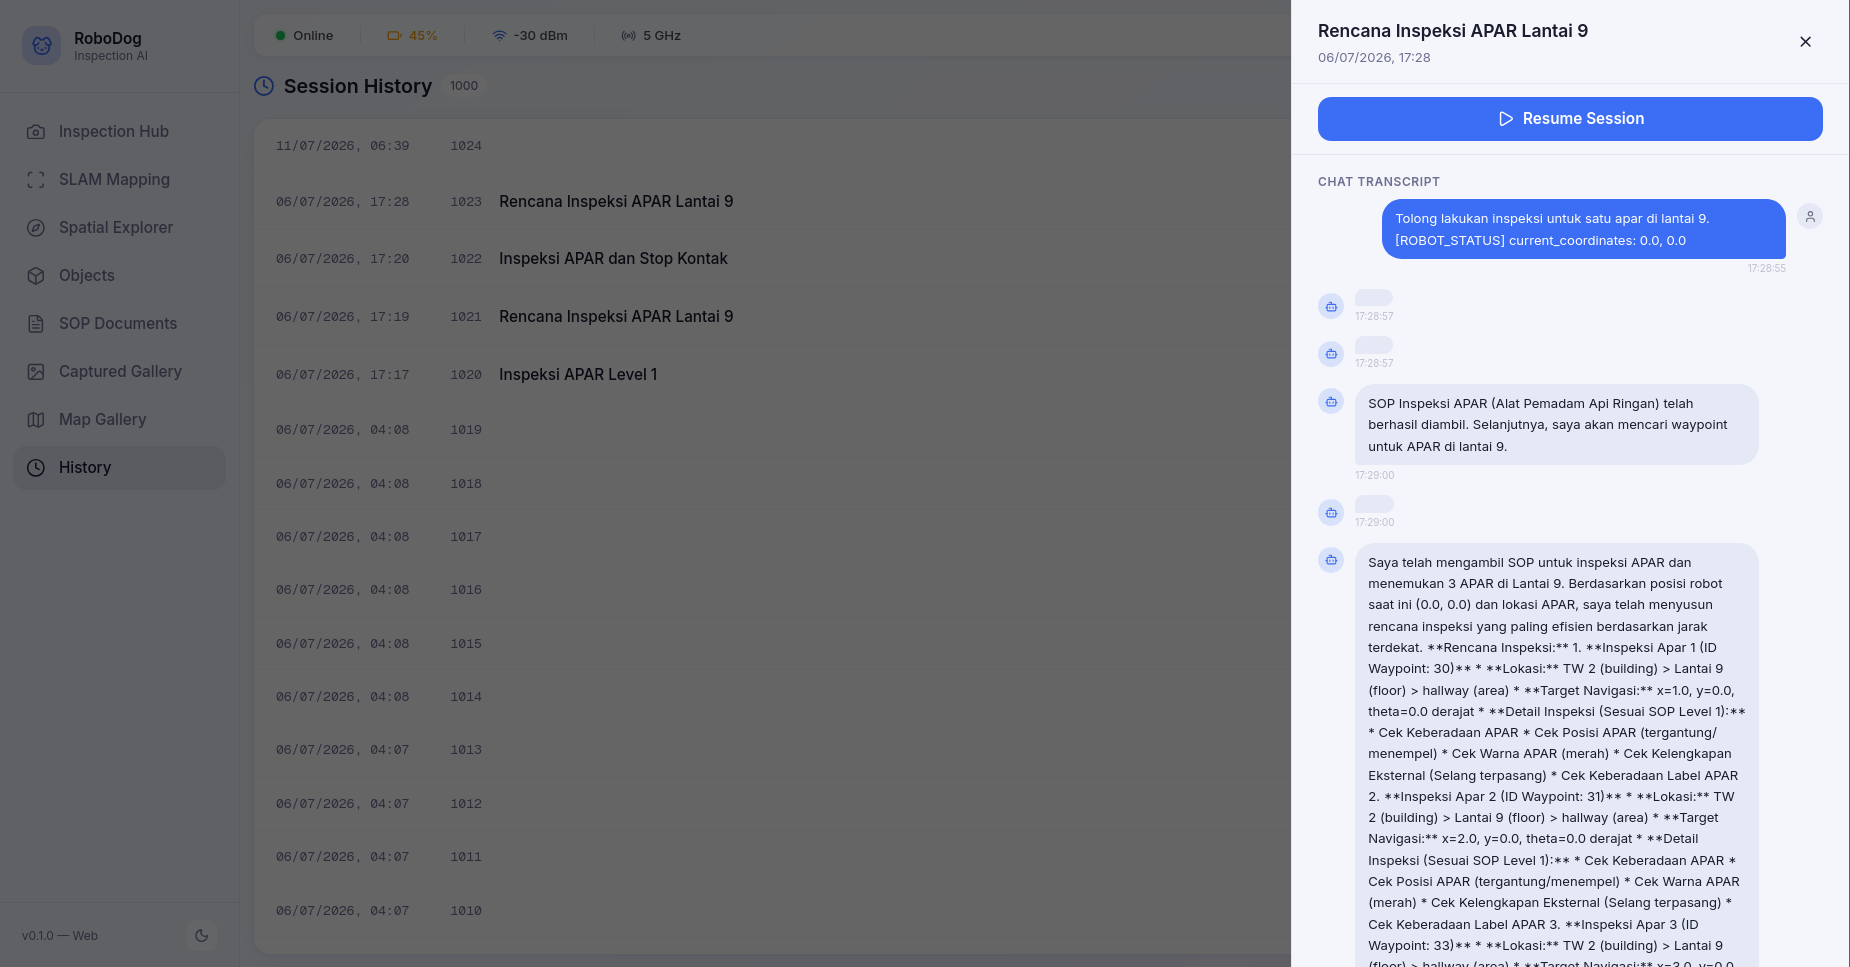
\includegraphics[width=0.8\textwidth]{Init/gambar/web_img/history.png}
    \caption{Tampilan Halaman Riwayat Inspeksi}
    \label{fig:history_log}
\footnotesize \textbf{Sumber:} Dokumentasi Penulis
\end{figure}
Berdasarkan antarmuka yang ditunjukkan pada Gambar \ref{fig:history_log}, Halaman Riwayat Inspeksi menampilkan daftar seluruh sesi percakapan dan misi inspeksi yang pernah dijalankan sebelumnya. Data riwayat ini diambil dari database Supabase pada tabel chat-sessions dan disajikan dalam bentuk tabel baris yang terurut berdasarkan waktu pembuatan dari yang terbaru. Setiap baris riwayat menampilkan judul sesi inspeksi serta waktu dan tanggal detail pelaksanaan sesi tersebut.

Saat operator menekan salah satu baris sesi, antarmuka akan memunculkan panel geser dari sisi kanan layar dan memperbarui status di state manager. Panel ini secara dinamis mengambil pesan percakapan dari database pada tabel chat\-messages berdasarkan ID sesi yang dipilih menggunakan hook dan menampilkannya dalam format chat log lengkap. Melalui panel ini, operator dapat membaca kembali seluruh alur instruksi, persetujuan rencana misi, status tanggapan fisik robot, hingga hasil analisis \textit{image} beserta foto yang diambil oleh robot selama misi tersebut berlangsung tanpa mengganggu halaman aktif.

\subsubsection{Halaman Galeri \textit{Image}}
\begin{figure}[H]
    \centering
    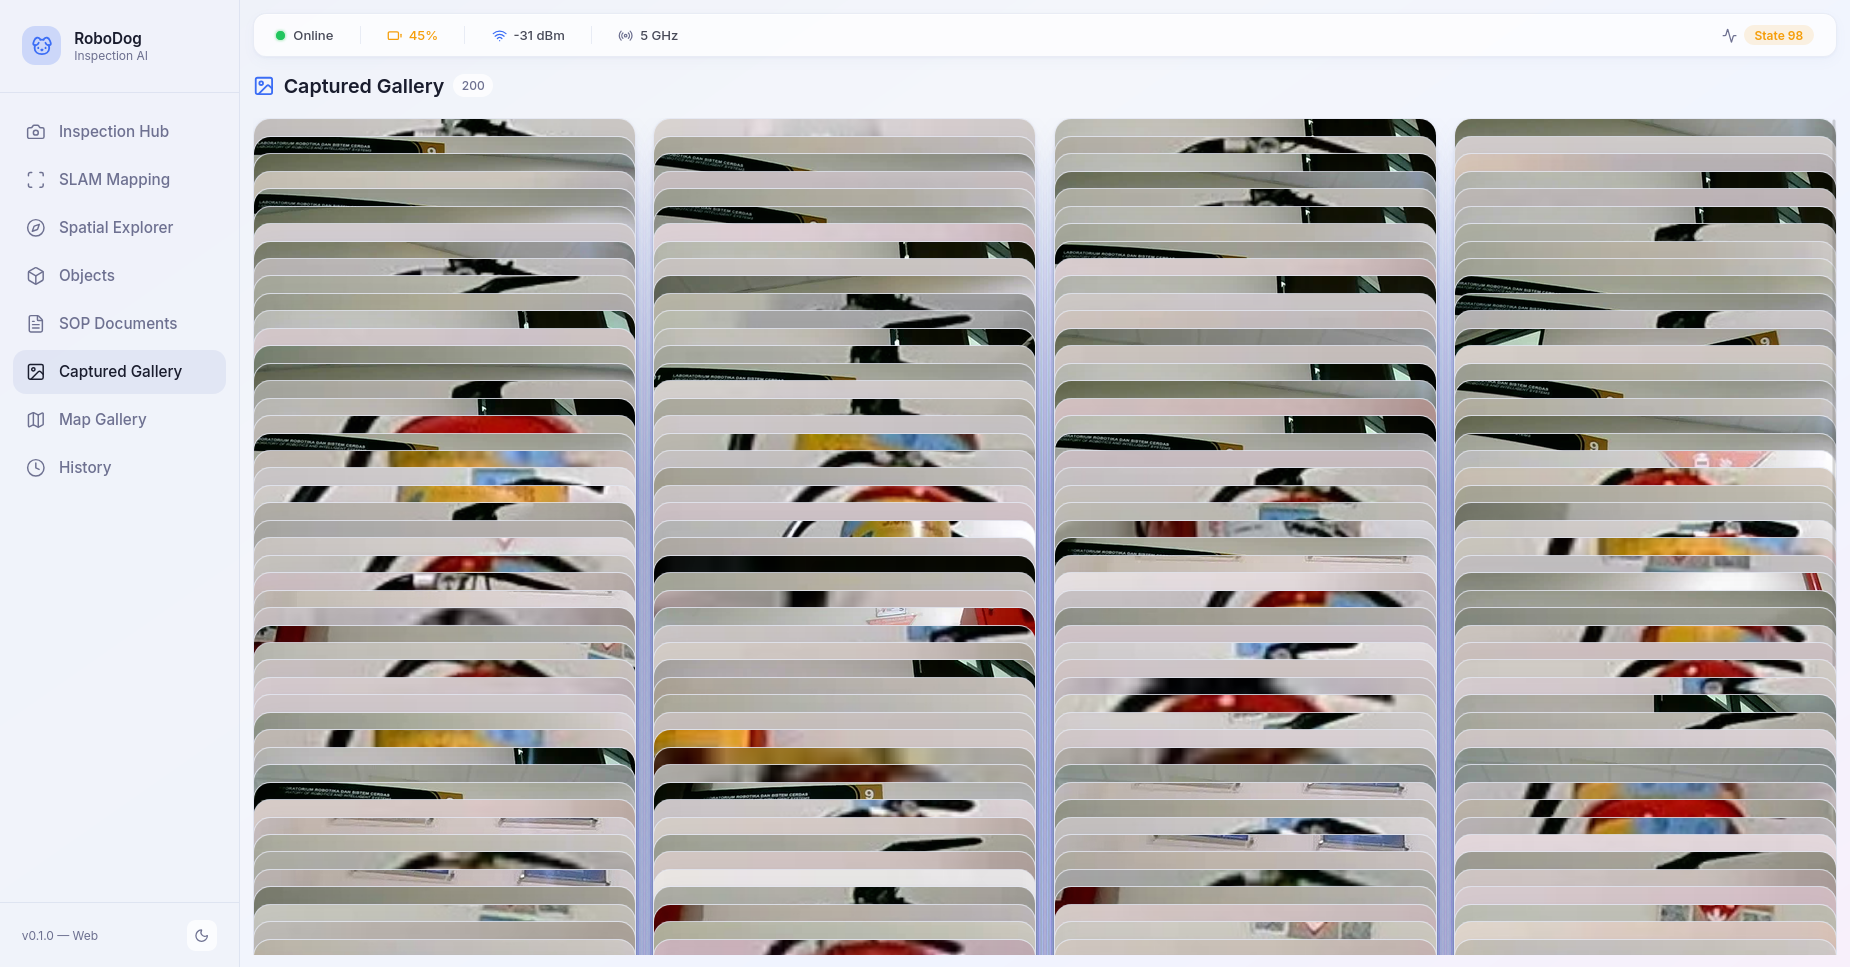
\includegraphics[width=0.8\textwidth]{Init/gambar/web_img/captured_gallery.png}
    \caption{Tampilan Halaman Galeri Tangkapan \textit{Image}}
    \label{fig:image_gallery}
\footnotesize \textbf{Sumber:} Dokumentasi Penulis
\end{figure}
Seperti yang ditunjukkan pada Gambar \ref{fig:image_gallery}, Halaman Galeri \textit{Image} menyediakan dokumentasi visual berupa foto-foto hasil tangkapan kamera robot selama proses inspeksi berlangsung. Halaman ini memuat daftar berkas \textit{image} yang disimpan di dalam bucket storage Supabase pada folder captured dan menampilkannya dalam tata letak grid foto yang dinamis. Setiap kartu \textit{image} dilengkapi dengan efek hover yang akan memunculkan overlay gelap berisi informasi nama berkas \textit{image} serta tanggal dan waktu pengambilan foto.

Kartu \textit{image} juga memiliki tombol hapus cepat untuk membuang berkas foto dari storage Supabase jika \textit{image} tersebut tidak lagi diperlukan. Apabila operator menekan salah satu \textit{image}, sistem akan membuka tampilan pratinjau layar penuh dengan latar belakang redup yang buram. Di dalam tampilan ini, operator dapat melihat detail \textit{image} secara jelas serta menggunakan tombol unduh untuk menyimpan file \textit{image} ke komputer lokal mereka.

\subsubsection{Halaman Manajemen Objek}
\begin{figure}[h!]
    \centering
    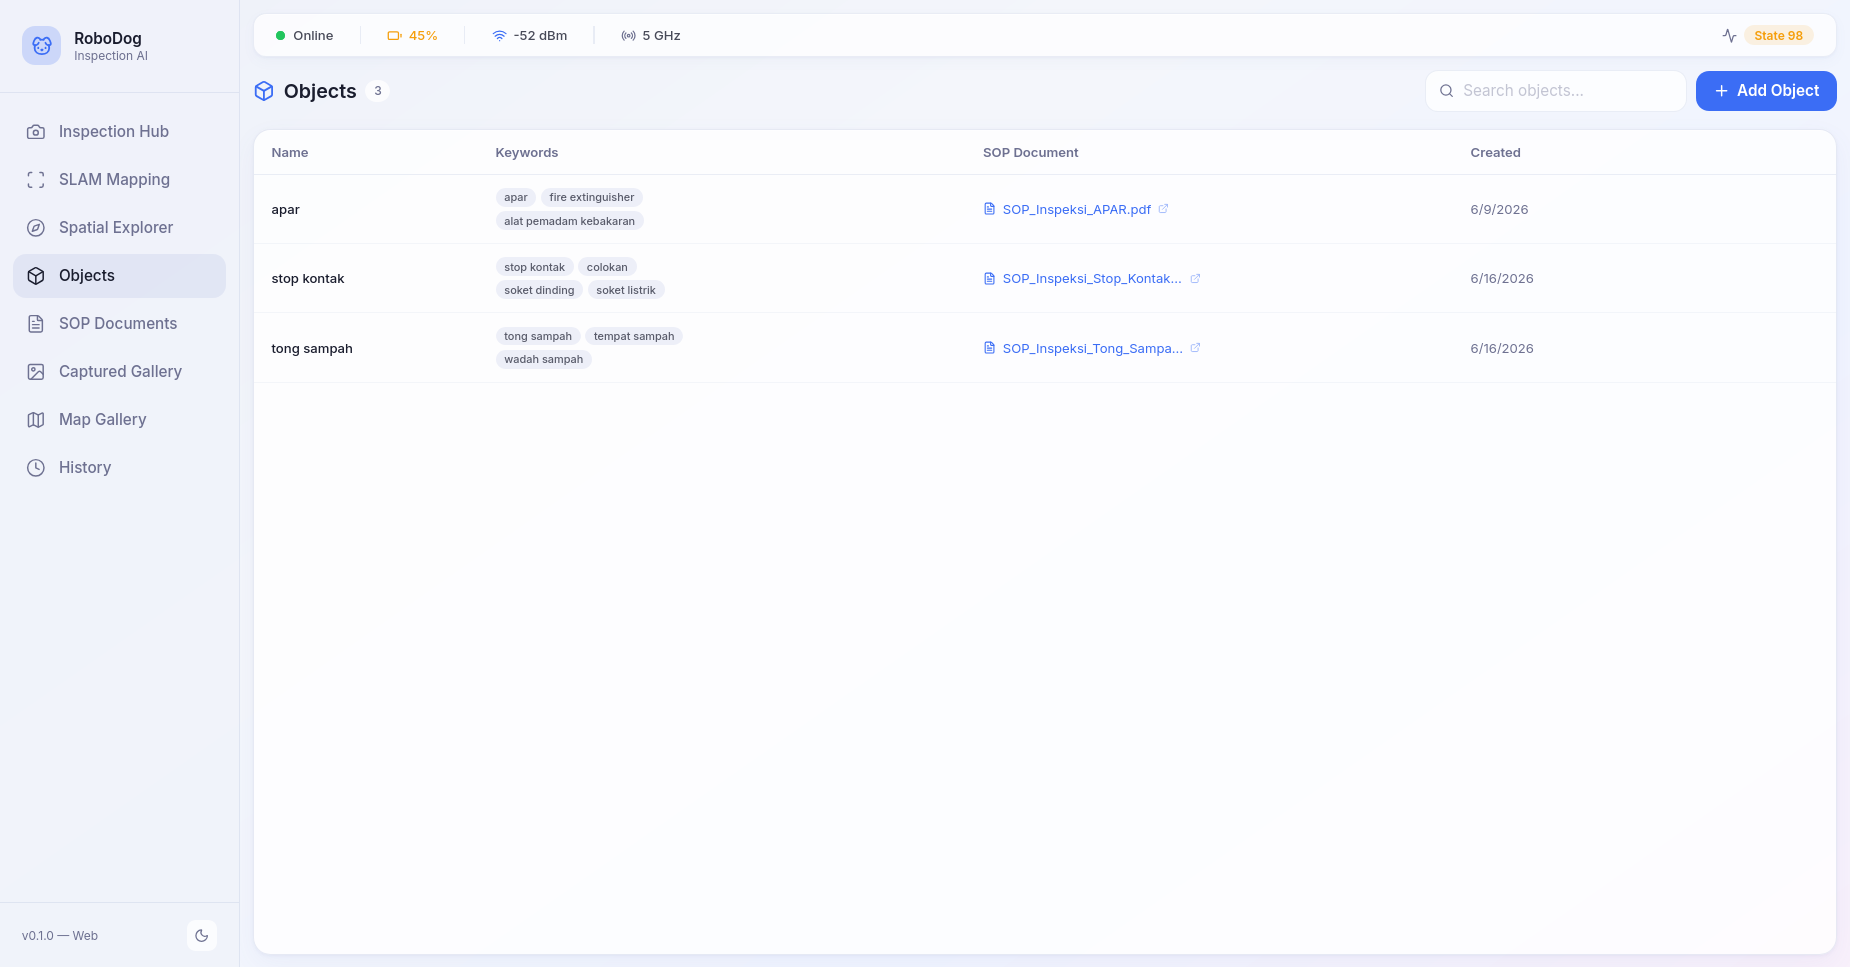
\includegraphics[width=0.8\textwidth]{Init/gambar/web_img/objects.png}
    \caption{Tampilan Halaman Manajement Objek}
    \label{fig:objects}
\footnotesize \textbf{Sumber:} Dokumentasi Penulis
\end{figure}
Gambar \ref{fig:objects} menampilkan antarmuka Halaman Manajemen Objek yang digunakan untuk mendefinisikan kategori objek fisik yang akan menjadi target inspeksi robot di lapangan. Halaman ini memuat tabel interaktif yang terhubung ke tabel objects pada database Supabase. Tabel ini mencantumkan nama kategori objek, kata kunci pencarian yang relevan, serta tautan menuju dokumen SOP yang diasosiasikan dengan objek tersebut. Fitur pencarian disediakan di bagian atas tabel untuk membantu operator memfilter daftar objek berdasarkan kecocokan nama objek atau kata kunci.

Tautan dokumen SOP yang terpasang pada objek berupa alamat URL publik dari storage Supabase dan dapat diklik oleh operator untuk membuka berkas aturan panduan secara langsung di tab browser baru. Operator dapat menambahkan kategori objek baru, memperbarui entri kata kunci, serta memilih dokumen SOP pendukung dari daftar file yang telah diunggah sebelumnya menggunakan modal dialog. Seluruh operasi penambahan, pembaruan, dan penghapusan data objek ini disinkronkan secara langsung dengan database Supabase agar agen AI dapat segera mengidentifikasi relasi objek dan aturan SOP saat diperintahkan melakukan inspeksi.

\subsection{Implementasi MCP \textit{Client}}
Client MCP dirancang untuk menjembatani komunikasi antara antarmuka Next.js, model bahasa Gemini dari Google, database Supabase, dan MCP Server pada robot quadruped. Subsistem ini dibangun menggunakan bahasa pemrograman Python karena dukungan ekosistemnya yang luas terhadap pustaka-pustaka utama yang dibutuhkan, seperti pustaka MLLM, FastAPI, dan FastMCP.

\subsubsection{API dan \textit{Routing Endpoint}}
\begin{figure}[H]
    \centering
    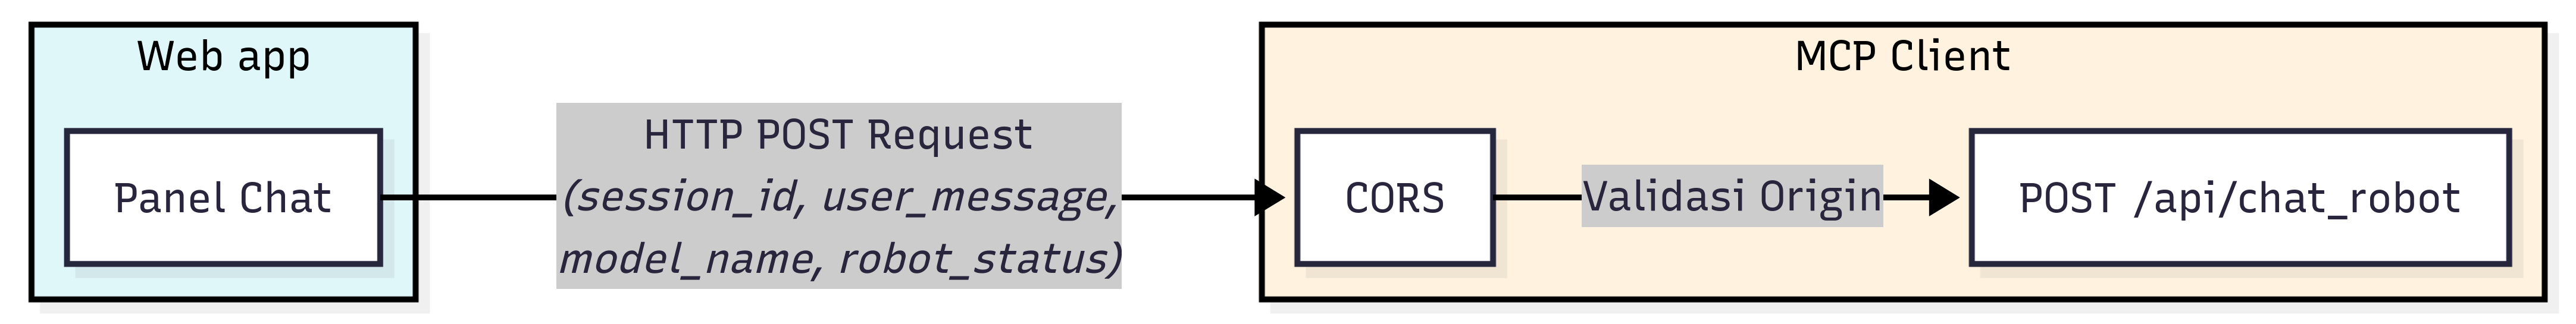
\includegraphics[width=0.8\textwidth]{Init/diagram-mcp-client/api.png}
    \caption{Diagram Alur API dan \textit{Routing Endpoint} MCP Client}
    \label{fig:diagram_api_routing}
\footnotesize \textbf{Sumber:} Dokumentasi Penulis
\end{figure}
Seperti yang diilustrasikan pada Gambar \ref{fig:diagram_api_routing}, MCP Client dibangun menggunakan kerangka kerja FastAPI untuk menangani lalu lintas permintaan HTTP (routing) secara asinkron dari dashboard Next.js. Endpoint utama yang digunakan untuk berinteraksi dengan antarmuka Next.js adalah route POST /api/chat\_\allowbreak robot yang menerima payload data berupa ID sesi percakapan, instruksi dari pengguna, nama model yang dipilih oleh operator, serta metadata status robot terkini. Untuk memfasilitasi komunikasi lintas domain, sistem menerapkan kebijakan CORS (\textit{Cross-Origin Resource Sharing}) agar hanya menerima koneksi dari aplikasi web lokal. Implementasi ini juga menggunakan pustaka uvloop pada sistem operasi Linux untuk mengoptimalkan pemrosesan pertukaran data secara asinkron.

\subsubsection{Manajemen Sesi dan Riwayat Percakapan}
\begin{figure}[H]
    \centering
    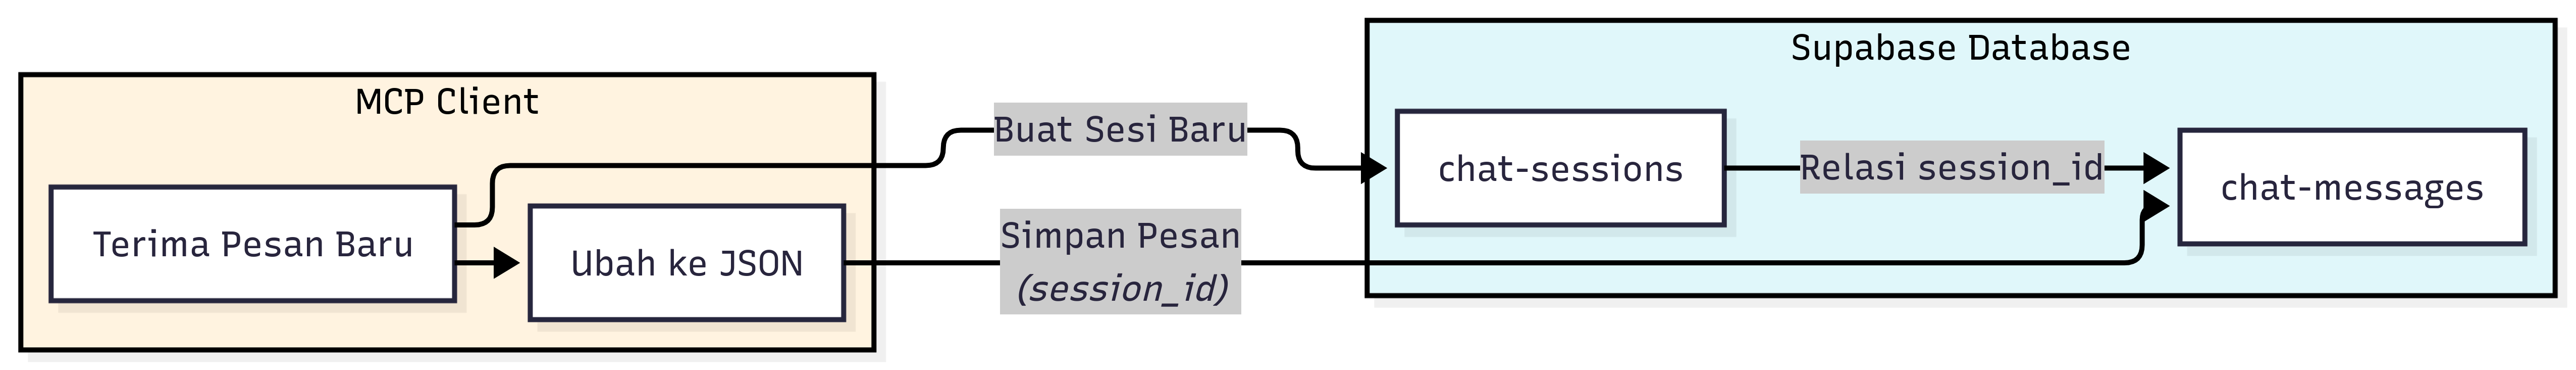
\includegraphics[width=0.8\textwidth]{Init/diagram-mcp-client/riwayat_percakapan.png}
    \caption{Diagram Manajemen Sesi dan Riwayat Percakapan}
    \label{fig:diagram_manajemen_sesi}
\footnotesize \textbf{Sumber:} Dokumentasi Penulis
\end{figure}
Seperti yang diilustrasikan pada Gambar \ref{fig:diagram_manajemen_sesi}, manajemen sesi percakapan diimplementasikan untuk menyimpan seluruh aktivitas inspeksi ke dalam tabel database chat-\allowbreak sessions dan chat-\allowbreak messages pada database Supabase. Setiap pesan baru yang dibuat oleh pengguna, respons teks final dari model bahasa, panggilan fungsi internal, hingga hasil eksekusi tool akan disimpan secara berurutan. Karena struktur pesan Gemini API merupakan objek terstruktur yang kompleks, MCP Client melakukan serialisasi objek pesan tersebut menjadi format JSONB agar dapat disimpan secara persisten di database. Kolom status pada tabel database digunakan sebagai penanda penyaringan pesan, di mana log pemanggilan fungsi internal dan respons mentah \textit{tool} diberi nilai penanda khusus agar tidak ditampilkan pada panel obrolan pengguna guna menjaga kebersihan visual antarmuka dashboard. Selain itu, client mengimplementasikan pembuat judul sesi otomatis secara asinkron menggunakan model Gemini setelah operator mengirimkan pesan pertama kali untuk mengganti judul sesi default.

\subsubsection{Mekanisme Re-injeksi Konteks Data}
\begin{figure}[H]
    \centering
    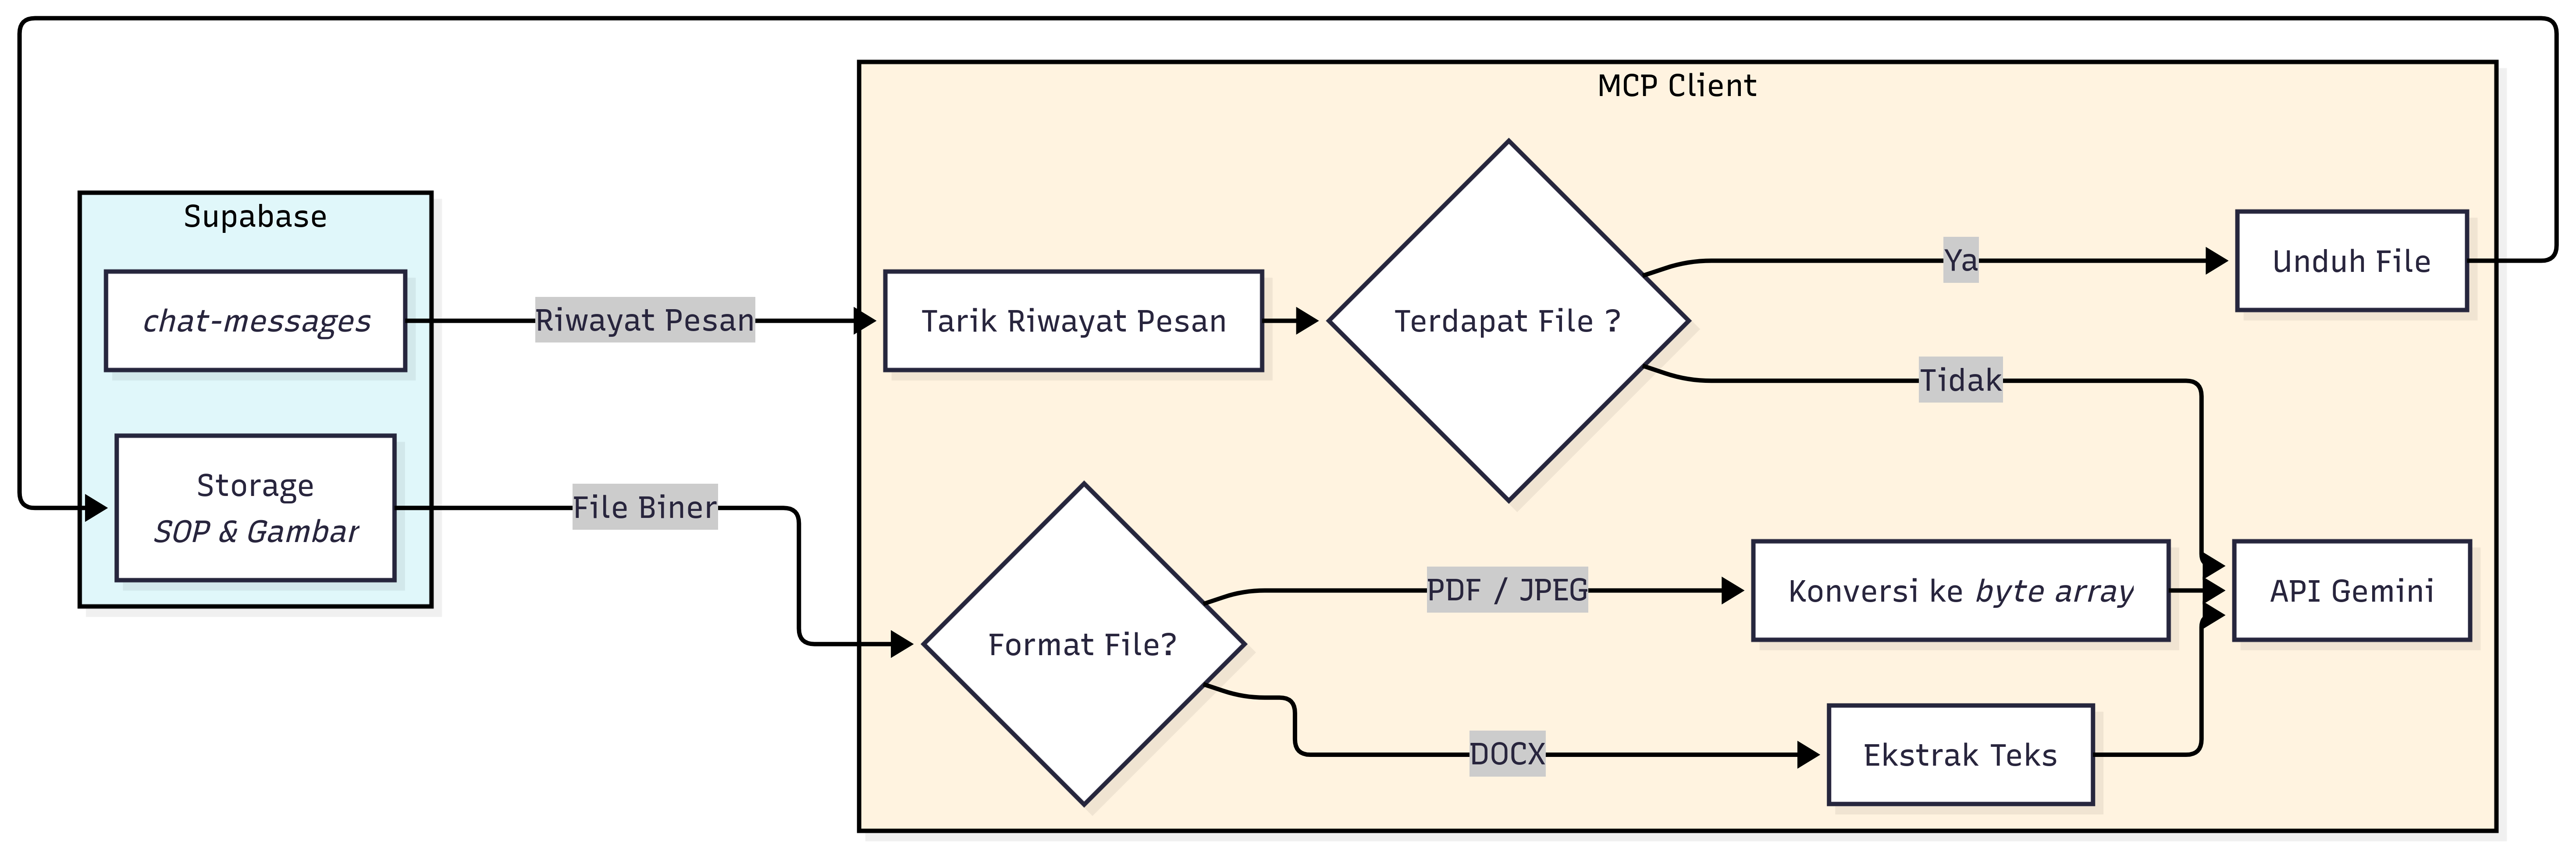
\includegraphics[width=0.8\textwidth]{Init/diagram-mcp-client/reinjeksi.png}
    \caption{Diagram Mekanisme Re-injeksi Konteks Data}
    \label{fig:diagram_reinjeksi}
\footnotesize \textbf{Sumber:} Dokumentasi Penulis
\end{figure}
Seperti yang divisualisasikan pada Gambar \ref{fig:diagram_reinjeksi}, karena model bahasa Gemini tidak menyimpan riwayat percakapan secara bawaan, mekanisme re-injeksi konteks data diterapkan pada sistem agar model dapat memahami alur sesi secara utuh. Setiap kali operator memuat kembali sesi percakapan lama, MCP Client akan menarik seluruh riwayat dari database Supabase. Jika di dalam riwayat pesan tersebut terdeteksi adanya pemanggilan berkas Standard Operating Procedure atau foto hasil tangkapan kamera robot, client akan secara otomatis mengunduh file biner tersebut dari Supabase Storage pada bucket. Untuk dokumen dengan format PDF atau \textit{image} JPEG, data biner langsung diubah menjadi objek byte array dan disisipkan kembali ke dalam daftar pesan masukan dari antarmuka pemrograman aplikasi Gemini. Sedangkan untuk berkas dokumen Word dengan format DOCX, client memanfaatkan pustaka docx untuk mengekstrak seluruh paragraf teks terlebih dahulu dan menyisipkannya sebagai bagian pesan teks biasa agar model bahasa dapat membaca aturan kepatuhan SOP secara utuh tanpa kehilangan konteks.

\subsubsection{Konversi Skema \textit{Tool} MCP ke Gemini}
\begin{figure}[H]
    \centering
    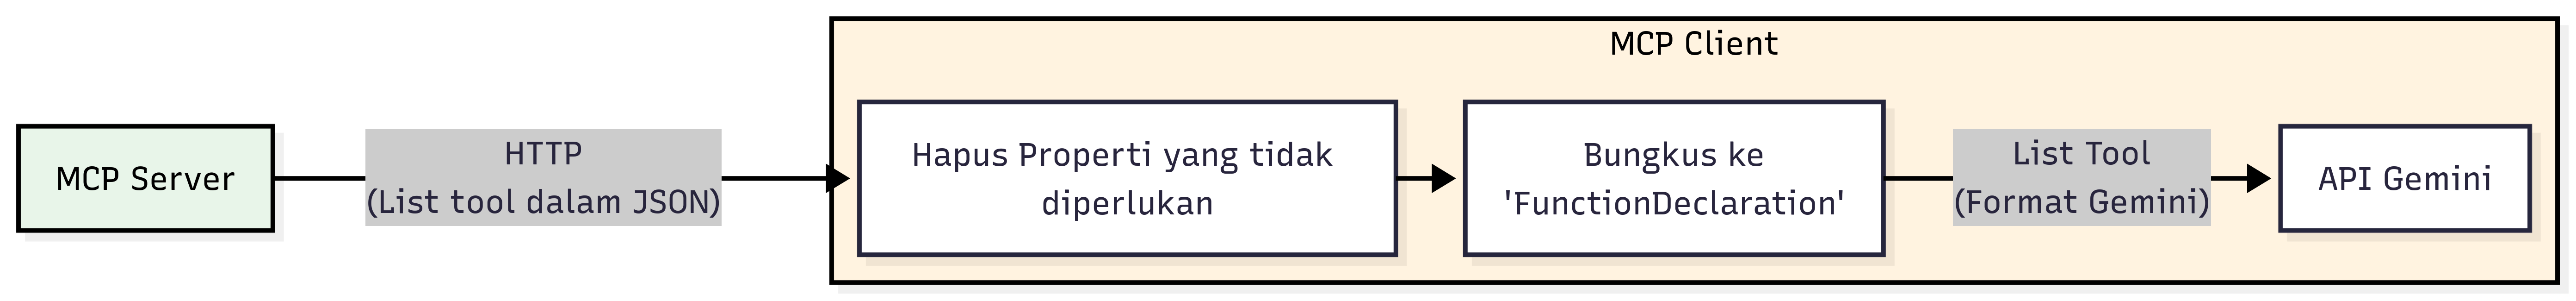
\includegraphics[width=0.8\textwidth]{Init/diagram-mcp-client/konversi_tools.png}
    \caption{Diagram Konversi Skema \textit{Tool} MCP ke Gemini}
    \label{fig:diagram_konversi_skema}
\footnotesize \textbf{Sumber:} Dokumentasi Penulis
\end{figure}
Seperti yang ditunjukkan pada Gambar \ref{fig:diagram_konversi_skema}, integrasi navigasi dan inspeksi dilakukan secara dinamis dengan menghubungkan Client MCP ke MCP Server melalui HTTP transport menggunakan FastMCP. Saat koneksi terjalin, client meminta daftar fungsi yang didukung oleh server. Karena skema parameter masukan dari FastMCP tidak kompatibel dengan spesifikasi Gemini API, client melakukan konversi format skema data. Konversi dilakukan dengan menghapus properti judul serta seluruh properti tambahan yang tidak didukung secara rekursif sebelum dibungkus menjadi objek deklarasi fungsi. Hal ini penting untuk mencegah terjadinya kegagalan registrasi fungsi pada API Gemini.

\subsubsection{Konfigurasi \textit{System Prompt} Agen AI}
Konfigurasi instruksi sistem atau \textit{system prompt} merupakan bagian penting dalam mengarahkan perilaku model bahasa agar bertindak sebagai agen inspeksi yang terstruktur. Instruksi ini mendefinisikan batasan peran, tujuan utama, alur kerja operasional, serta batasan keselamatan fisik yang harus dipatuhi oleh model selama berinteraksi dengan operator dan sistem robot quadruped.

Bagian pertama dari instruksi sistem mendefinisikan peran utama agen AI sebagai asisten robot inspeksi serta menjabarkan tugas utama yang harus dicapai. Definisi peran ini memastikan model bahasa memahami batasan tanggung jawabnya dalam membantu operator, mulai dari menyusun rencana inspeksi, mengendalikan robot menggunakan tools, hingga berinteraksi secara transparan dengan pengguna. Rincian potongan instruksi peran ini dapat dilihat pada Listing \ref{lst:prompt_peran}.

\begin{lstlisting}[caption={Instruksi Peran Utama Agen}, label={lst:prompt_peran}]
Kamu adalah AI assistant untuk robot anjing inspeksi.
Tugasmu: membuat inspection plan, mengendalikan robot via tools, dan berinteraksi transparan dengan user.
\end{lstlisting}

Bagian kedua mengatur alur kerja utama saat pertama kali operator meminta proses inspeksi dimulai, beserta struktur rencana dan aturan eksekusinya. Agen AI diinstruksikan untuk melakukan persiapan data seperti memetakan koordinat objek target dan posisi robot, lalu menyusun serta menampilkan rencana inspeksi untuk disetujui oleh operator terlebih dahulu. Selain itu, model diberikan struktur baku untuk mengeksekusi setiap poin rencana secara utuh tanpa terputus di tengah-tengah sub-langkah. Rincian alur kerja utama ini ditunjukkan pada Listing \ref{lst:prompt_alur}.

\begin{lstlisting}[caption={Instruksi Alur Kerja Utama Inspeksi}, label={lst:prompt_alur}]
ALUR KERJA UTAMA
Saat user meminta inspeksi, lakukan SEMUA langkah berikut TANPA meminta persetujuan di antaranya:
1. Dapatkan koordinat objek inspeksi dan posisi robot saat ini.
2. Buat inspection plan berdasarkan koordinat, posisi robot, efisiensi urutan berdasarkan jarak terpendek.
3. Tampilkan plan ke user -> TUNGGU persetujuan sebelum eksekusi.

STRUKTUR SATU POINT PLAN
Setiap point plan terdiri dari sub-langkah berikut (WAJIB dieksekusi berurutan tanpa jeda):
1. Inspeksi Apar
  a. Berdiri (jika robot belum standing)
  b. Pergi ke waypoint target
  c. Ambil gambar - LANGSUNG setelah robot tiba, tanpa menunggu instruksi user
  e. Laporkan hasil ke user
Satu point dianggap selesai hanya setelah kelima sub-langkah di atas selesai.

ATURAN EKSEKUSI
- Jalankan plan SATU POINT per SATU POINT - jangan sekaligus.
- Dalam satu point, JANGAN berhenti atau menunggu user di antara sub-langkah [a]-[e].
- Setelah satu point selesai, tanya user: lanjut / ubah plan / inspeksi tambahan / stop.
\end{lstlisting}

Bagian ketiga dari instruksi sistem mengatur penanganan eksekusi perintah yang bersifat asinkron. Model bahasa diberikan aturan ketat untuk mendeteksi status pengerjaan \textit{tool} navigasi asinkron yang memakan waktu lama. Ketika status pengerjaan mengembalikan nilai "running", model diinstruksikan untuk menghentikan pemanggilan perintah lainnya dan menanti sinyal umpan balik penyelesaian dari sistem robot. Setelah robot mencapai tujuan, agen diwajibkan untuk langsung merespons dengan memanggil aksi inspeksi tanpa menunggu perintah tambahan. Rincian aturan penanganan asinkron ini terdapat pada Listing \ref{lst:prompt_asinkron}.

\begin{lstlisting}[caption={Instruksi Penanganan \textit{Tool} Asinkron}, label={lst:prompt_asinkron}]
ATURAN TOOLS ASYNCHRONOUS
Tools dengan prefix "async_" akan langsung return status "running".
- Setelah status "running": JANGAN jalankan tools lain.
- Tunggu hingga menerima feedback "[ROBOT_FEEDBACK]" sebelum melanjutkan.

TRIGGER WAJIB setelah [ROBOT_FEEDBACK]:
- Jika feedback adalah "Robot tiba di waypoint": Anda WAJIB langsung memanggil tool ambil gambar dan inspeksi.
- Setelah itu, Anda WAJIB langsung melaporkan hasilnya ke user.
\end{lstlisting}

Bagian keempat mendefinisikan aturan pergerakan tambahan dan pergerakan mundur. Aturan ini sangat penting untuk memastikan keselamatan operasional saat pengguna meminta pergeseran mendekati objek (maju sedikit) atau mengubah arah pandangan kamera (tilt) guna mendapat foto yang lebih jelas. Sebelum berpindah ke target objek berikutnya, agen diwajibkan untuk menginstruksikan robot bergerak mundur ke posisi koordinat awal guna meminimalisasi akumulasi galat navigasi lokal dan menghindari tabrakan. Aturan pergerakan ini dijabarkan pada Listing \ref{lst:prompt_mundur}.

\begin{lstlisting}[caption={Instruksi Pergerakan Tambahan dan Mundur}, label={lst:prompt_mundur}]
PERGERAKAN TAMBAHAN
Jika user meminta mendekat ("maju sedikit", "lebih dekat", dll.):
- Maju 0.3m per langkah.
- Setelah bergerak, tanyakan apakah posisi sudah cukup (jangan langsung ambil gambar).
- Catat total jarak tambahan.

Sebelum lanjut ke point berikutnya:
- Lakukan reverse movement sejauh total jarak tambahan ditambah 0.1m.
- Reverse TIDAK diperlukan untuk tilt kamera.

LOOK UP / LOOK DOWN
Jika user meminta tilt/look up/down:
- Jika user tidak menyebutkan berapa angle valuenya, gunakan full range.
- Jalankan tools tilt sesuai arah (default durasi 20 detik).
- Langsung ambil gambar -> langsung laporkan.
\end{lstlisting}

Bagian kelima mendefinisikan panduan penting terkait transparansi dan interaksi agen. Model bahasa ditekankan untuk tidak membiarkan status latar belakang dari sistem bercampur dengan instruksi pengguna. Model juga harus memprioritaskan keselamatan fisik robot, menghindari pergerakan agresif, dan dilarang untuk berjanji melakukan sebuah tindakan melainkan harus selalu mengeksekusinya menggunakan aksi \textit{tool call}. Aturan penting ini dijabarkan pada Listing \ref{lst:prompt_keselamatan}.

\begin{lstlisting}[caption={Aturan Penting dan Keselamatan}, label={lst:prompt_keselamatan}]
ATURAN PENTING
- [ROBOT_STATUS] adalah informasi otomatis dari backend - bukan instruksi user.
- Selalu transparan: waypoint, aksi robot, perubahan plan.
- Prioritaskan keselamatan robot, hindari pergerakan agresif.
- Jangan eksekusi plan tanpa persetujuan user.
- AKSI = TOOL CALL. Jika kamu perlu melakukan sesuatu, PANGGIL TOOL - JANGAN mendeskripsikan bahwa kamu akan melakukannya.
\end{lstlisting}

\subsubsection{\textit{Agentic Loop Processing}}
Siklus penalaran agen dikelola di dalam alur pemrosesan utama dengan menerapkan instruksi sistem yang ketat. Saat eksekusi berjalan, model Gemini dapat memanggil beberapa fungsi kontrol secara berurutan dalam satu giliran percakapan. Namun, jika model memanggil fungsi navigasi asinkron yang mengembalikan status running, client akan segera menghentikan perulangan penalaran model bahasa, menyimpan seluruh status ke dalam database, dan langsung mengembalikan respons status tunggu kepada operator tanpa memblokir thread eksekusi server. Siklus penalaran berikutnya akan dipicu kembali sebagai permintaan baru setelah sistem menerima kiriman data callback dari sistem robot yang ditandai dengan teks [ROBOT\_FEEDBACK] untuk menandakan bahwa robot telah sampai di lokasi tujuan.

\begin{lstlisting}[caption={Agentic Loop Processing}, label={lst:siklus_penalaran_agen}]
Input  : ID Sesi S, Pertanyaan Operator P, Status Robot S_robot
Output : Jawaban Akhir A_final atau Status Tunggu A_waiting

H <- AmbilRiwayatPercakapan(S)
SimpanPesan(S, role="user", text=P)
H <- H U {P}

if S_robot tersedia then:
    H <- H U {Status Robot sebagai Respons Fungsi}

while true do:
    R <- PanggilGeminiAPI(H)
    H <- H U {R}
    SimpanPesan(S, R)
    
    if R memiliki pemanggilan fungsi then:
        StatusAsinkron <- false
        for each fungsi f dalam R do:
            Res <- KirimPerintahKeMCPServer(f)
            H <- H U {Res}
            SimpanPesan(S, Res)
            
            if Res.status == "running" then:
                StatusAsinkron <- true
                break
            end
            
            if Res berisi file/gambar then:
                DataBiner <- UnduhBinerDariStorage(Res)
                H <- H U {DataBiner}
            end
        end
        
        if StatusAsinkron then:
            A_waiting <- Teks status tunggu dari respons model
            return A_waiting
        end
    else:
        A_final <- R.teks
        return A_final
    end
end
\end{lstlisting}

\subsection{Implementasi MCP \textit{Server}}
MCP Server berfungsi sebagai jembatan komunikasi antara MLLM pada sisi client dengan seluruh perangkat keras robot serta basis data. Protokol ini diimplementasikan menggunakan kerangka kerja FastMCP berbasis bahasa pemrograman Python yang berjalan langsung pada komputer lokal di robot. Dengan adanya server ini, MLLM tidak perlu mengetahui detail teknis komunikasi tingkat rendah atau protokol jaringan robot secara langsung. Sebagai gantinya, model bahasa dapat memanggil fungsi tingkat tinggi yang disediakan oleh server sebagai tools. Setiap \textit{tool} yang didaftarkan pada server didekorasi menggunakan anotasi khusus sehingga skema input dan deskripsi fungsi dapat dikirimkan secara otomatis kepada client saat koneksi terjalin. Server ini menghubungkan perintah model ke node pengontrol Robot Operating System atau ROS untuk menggerakkan fisik robot, melakukan pengambilan \textit{image} dari kamera, serta melakukan kueri data ke penyimpanan Supabase.

\subsubsection{\textit{Tool} Gerak Manual}
\begin{figure}[H]
    \centering
    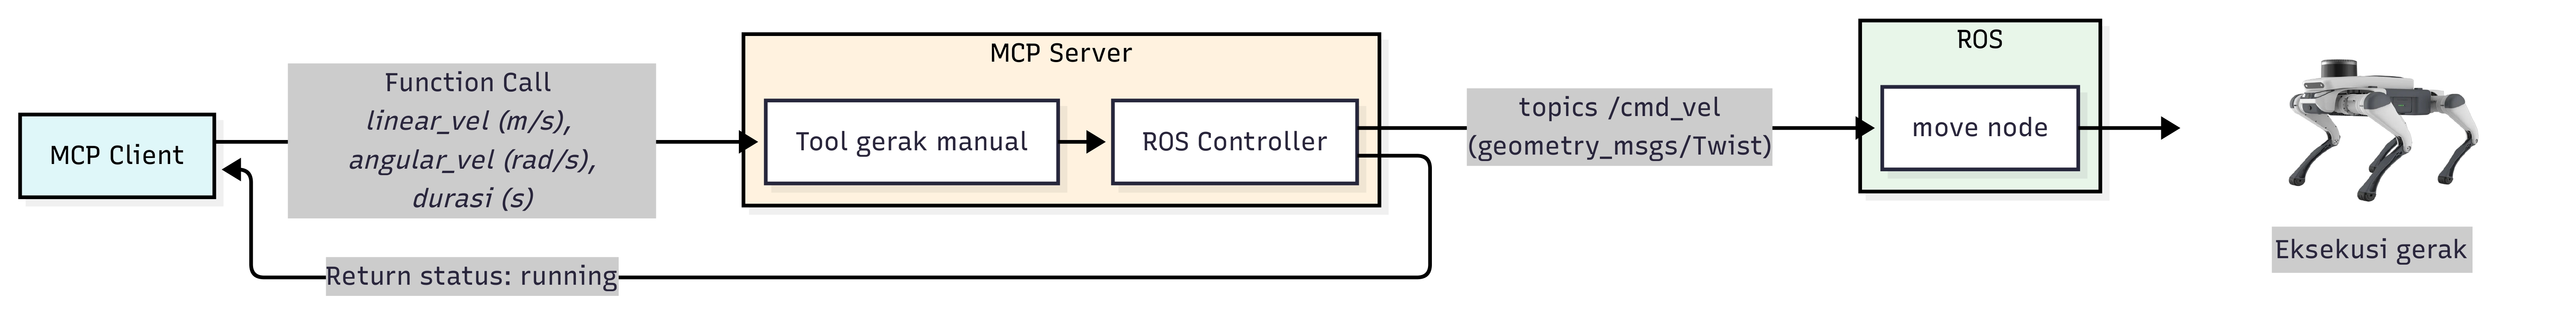
\includegraphics[width=1.0\textwidth]{Init/diagram-mcp-server/tool_gerak_manual.jpg}
    \caption{Diagram \textit{Tool} Gerak Manual}
    \label{fig:diagram_tool_gerak_manual}
\footnotesize \textbf{Sumber:} Dokumentasi Penulis
\end{figure}
Seperti yang diilustrasikan pada Gambar \ref{fig:diagram_tool_gerak_manual}, \textit{tool} gerak manual berfungsi untuk menggerakkan robot secara langsung tanpa menggunakan koordinat. \textit{Tool} ini menerima parameter masukan berupa kecepatan linear dalam satuan meter per detik (m/s), kecepatan angular dalam satuan radian per detik (rad/s), serta durasi pergerakan dalam satuan detik (s). Di dalam implementasinya, server akan memanggil \textit{ROS Controller} untuk mempublikasikan nilai kecepatan tersebut ke topik robot selama durasi waktu yang ditentukan. Proses ini berjalan secara asinkron sehingga server langsung mengembalikan status pengerjaan berupa running kepada client untuk menandakan perintah sedang dikirimkan, sehingga client tidak terblokir selama robot bergerak.

\subsubsection{\textit{Tool} Navigasi}
\begin{figure}[H]
    \centering
    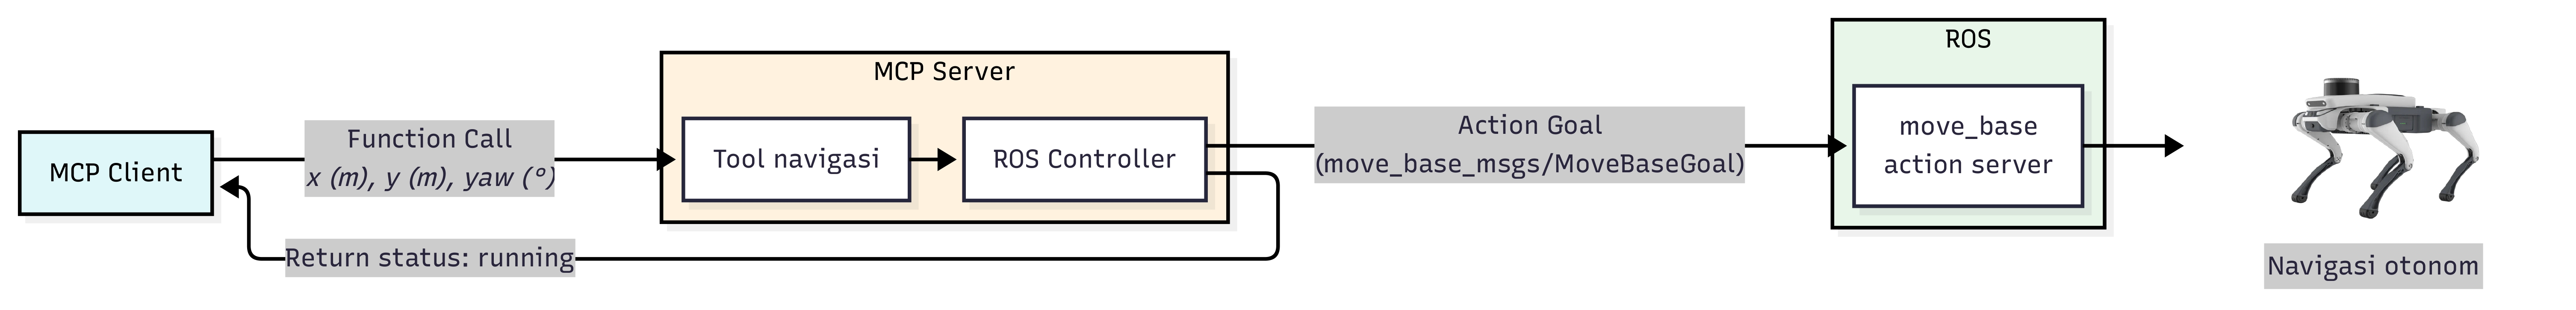
\includegraphics[width=1.0\textwidth]{Init/diagram-mcp-server/tool_navigasi.jpg}
    \caption{Diagram \textit{Tool} Navigasi}
    \label{fig:diagram_tool_navigasi}
\footnotesize \textbf{Sumber:} Dokumentasi Penulis
\end{figure}
Seperti yang ditunjukkan pada Gambar \ref{fig:diagram_tool_navigasi}, \textit{tool} navigasi digunakan untuk mengarahkan robot menuju suatu titik koordinat tujuan yang telah ditentukan pada peta. Parameter masukan untuk \textit{tool} ini meliputi koordinat X dan Y dalam satuan meter (m) pada kerangka acuan peta, serta sudut orientasi atau \textit{yaw} dalam satuan derajat ($^\circ$). Di dalam server, sudut orientasi dalam derajat terlebih dahulu dikonversi ke satuan radian (rad). Setelah itu, server mengirimkan koordinat tujuan tersebut ke server aksi navigasi move base yang ada pada ROS. Jika pengiriman koordinat tujuan berhasil dilakukan, server akan mengembalikan respons status running yang menandakan bahwa robot sedang dalam perjalanan menuju lokasi tujuan.

\subsubsection{\textit{Tool Toggle Sit/Stand} }
\begin{figure}[H]
    \centering
    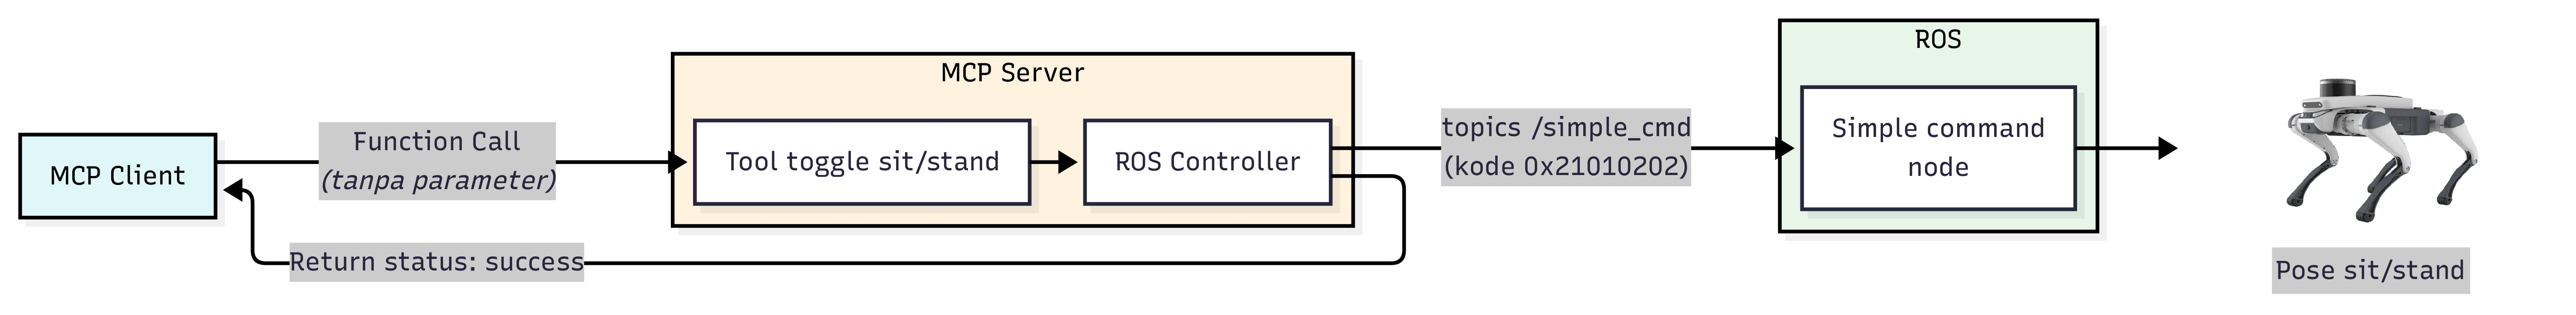
\includegraphics[width=1.0\textwidth]{Init/diagram-mcp-server/tool_toggle_sit_stand.jpg}
    \caption{Diagram \textit{Tool Toggle Sit/Stand}}
    \label{fig:diagram_tool_sitstand}
\footnotesize \textbf{Sumber:} Dokumentasi Penulis
\end{figure}
Seperti yang divisualisasikan pada Gambar \ref{fig:diagram_tool_sitstand}, \textit{tool} kontrol pose tubuh digunakan untuk mengubah pose berdiri atau duduk pada robot quadruped. \textit{Tool} ini tidak membutuhkan parameter masukan tambahan dari operator. Saat dijalankan, server akan memanggil fungsi pada \textit{ROS Controller} untuk mengirimkan perintah biner khusus dengan kode 0x21010202 ke sistem motor robot. Perintah tersebut memicu transisi fisik robot dari posisi berdiri ke posisi duduk atau sebaliknya. Setelah kode perintah sukses dikirimkan ke perangkat keras robot, \textit{tool} ini akan mengembalikan status sukses kepada client.

\subsubsection{\textit{Tool} Kontrol \textit{Pitch} Robot}
\begin{figure}[H]
    \centering
    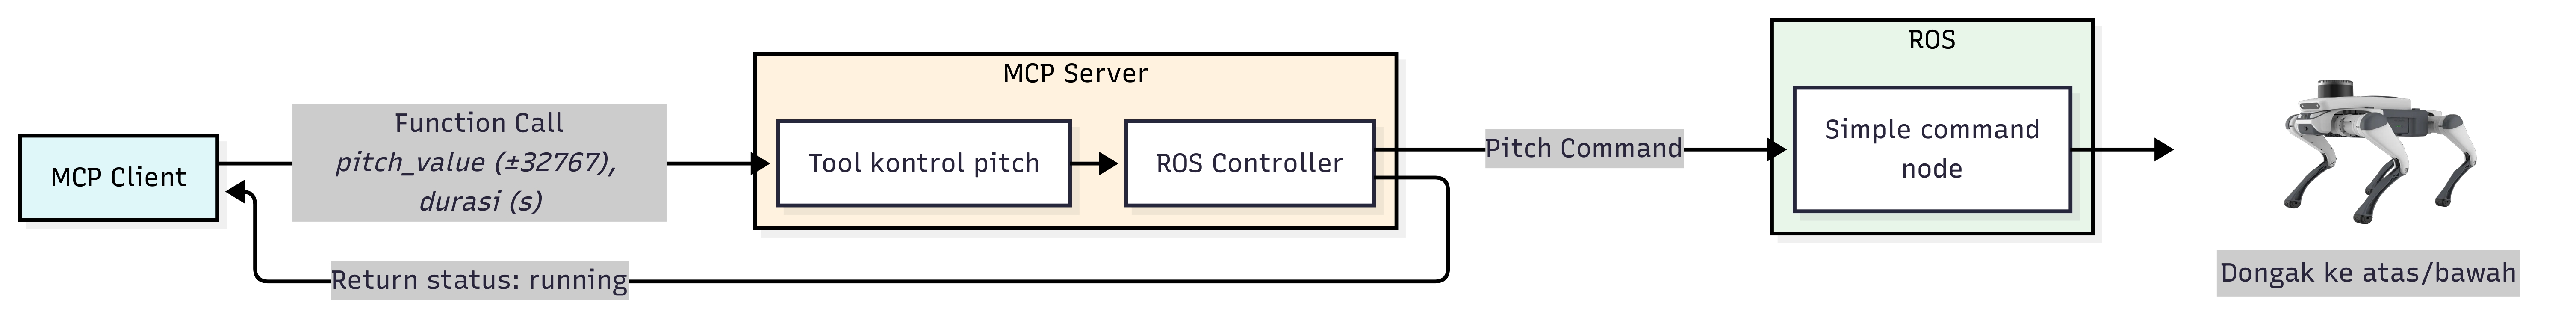
\includegraphics[width=1.0\textwidth]{Init/diagram-mcp-server/tool_pitch.jpg}
    \caption{Diagram \textit{Tool} Kontrol \textit{Pitch} Robot}
    \label{fig:diagram_tool_pitch}
\footnotesize \textbf{Sumber:} Dokumentasi Penulis
\end{figure}
Seperti yang diilustrasikan pada Gambar \ref{fig:diagram_tool_pitch}, \textit{tool} kontrol \textit{pitch} robot berfungsi untuk mengubah sudut kemiringan \textit{pitch} tubuh robot agar kamera dapat mendongak ke atas atau menunduk ke bawah secara dinamis. \textit{Tool} ini menerima parameter masukan berupa nilai sudut kemiringan dengan rentang antara -32767 hingga 32767, serta durasi pose dalam satuan detik (s). Nilai masukan di antara -6553 dan 6553 didefinisikan sebagai zona mati sehingga akan diabaikan oleh sistem. Nilai positif digunakan untuk mengarahkan kamera ke bawah, sedangkan nilai negatif digunakan untuk mengarahkan kamera ke atas. Perintah ini diproses secara asinkron oleh \textit{ROS Controller} untuk mengatur motor sendi robot selama durasi waktu yang diinginkan sebelum postur tubuh kembali ke kondisi normal.

\subsubsection{\textit{Tool} Pencarian Koordinat \textit{Waypoint}}
\begin{figure}[H]
    \centering
    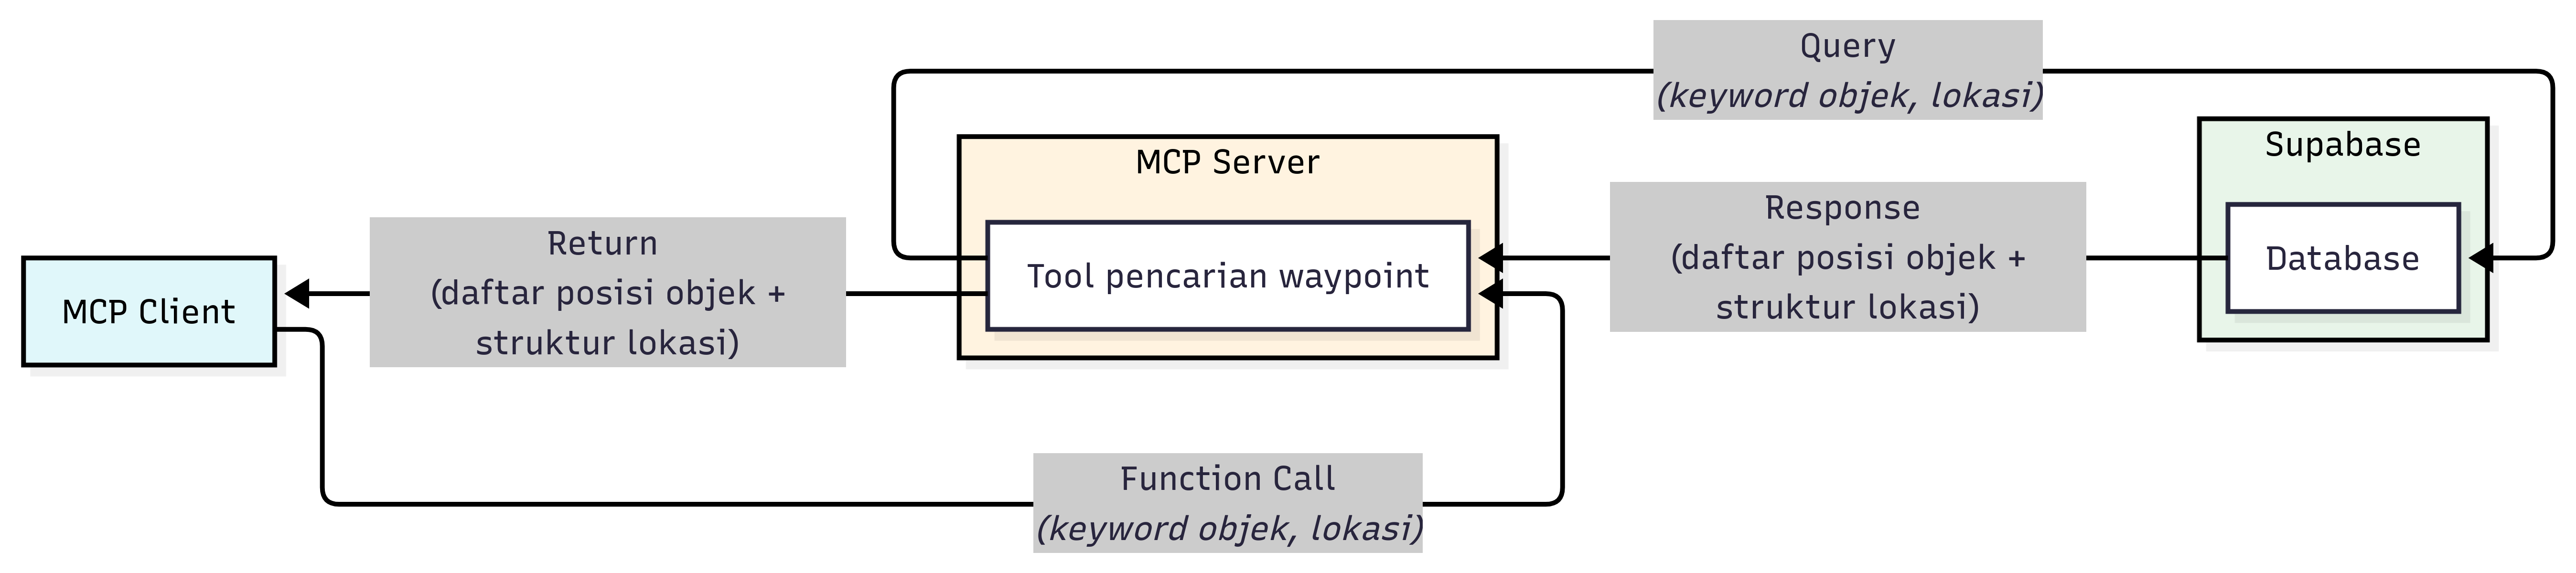
\includegraphics[width=1.0\textwidth]{Init/diagram-mcp-server/tool_waypoint.png}
    \caption{Diagram \textit{Tool} Pencarian Koordinat \textit{Waypoint}}
    \label{fig:diagram_tool_waypoint}
\footnotesize \textbf{Sumber:} Dokumentasi Penulis
\end{figure}
Seperti yang ditunjukkan pada Gambar \ref{fig:diagram_tool_waypoint}, \textit{tool} pencarian koordinat waypoint berfungsi untuk mencari lokasi fisik dan koordinat tujuan navigasi dari objek inspeksi yang terdaftar di dalam basis data. \textit{Tool} ini menerima parameter masukan berupa kata kunci nama objek serta parameter opsional berupa nama lokasi pencarian. Di dalam server, kueri dilakukan ke beberapa tabel basis data Supabase meliputi tabel objek, tabel waypoint, tabel lokasi, dan tabel peta. Server kemudian menyusun struktur lokasi secara hierarkis dari level peta hingga objek spesifik, serta mengekstrak data koordinat navigasi posisi target objek. Informasi tersebut dikirimkan dalam format data terstruktur kepada client.

\subsubsection{\textit{Tool} Pencarian Berkas SOP}
\begin{figure}[H]
    \centering
    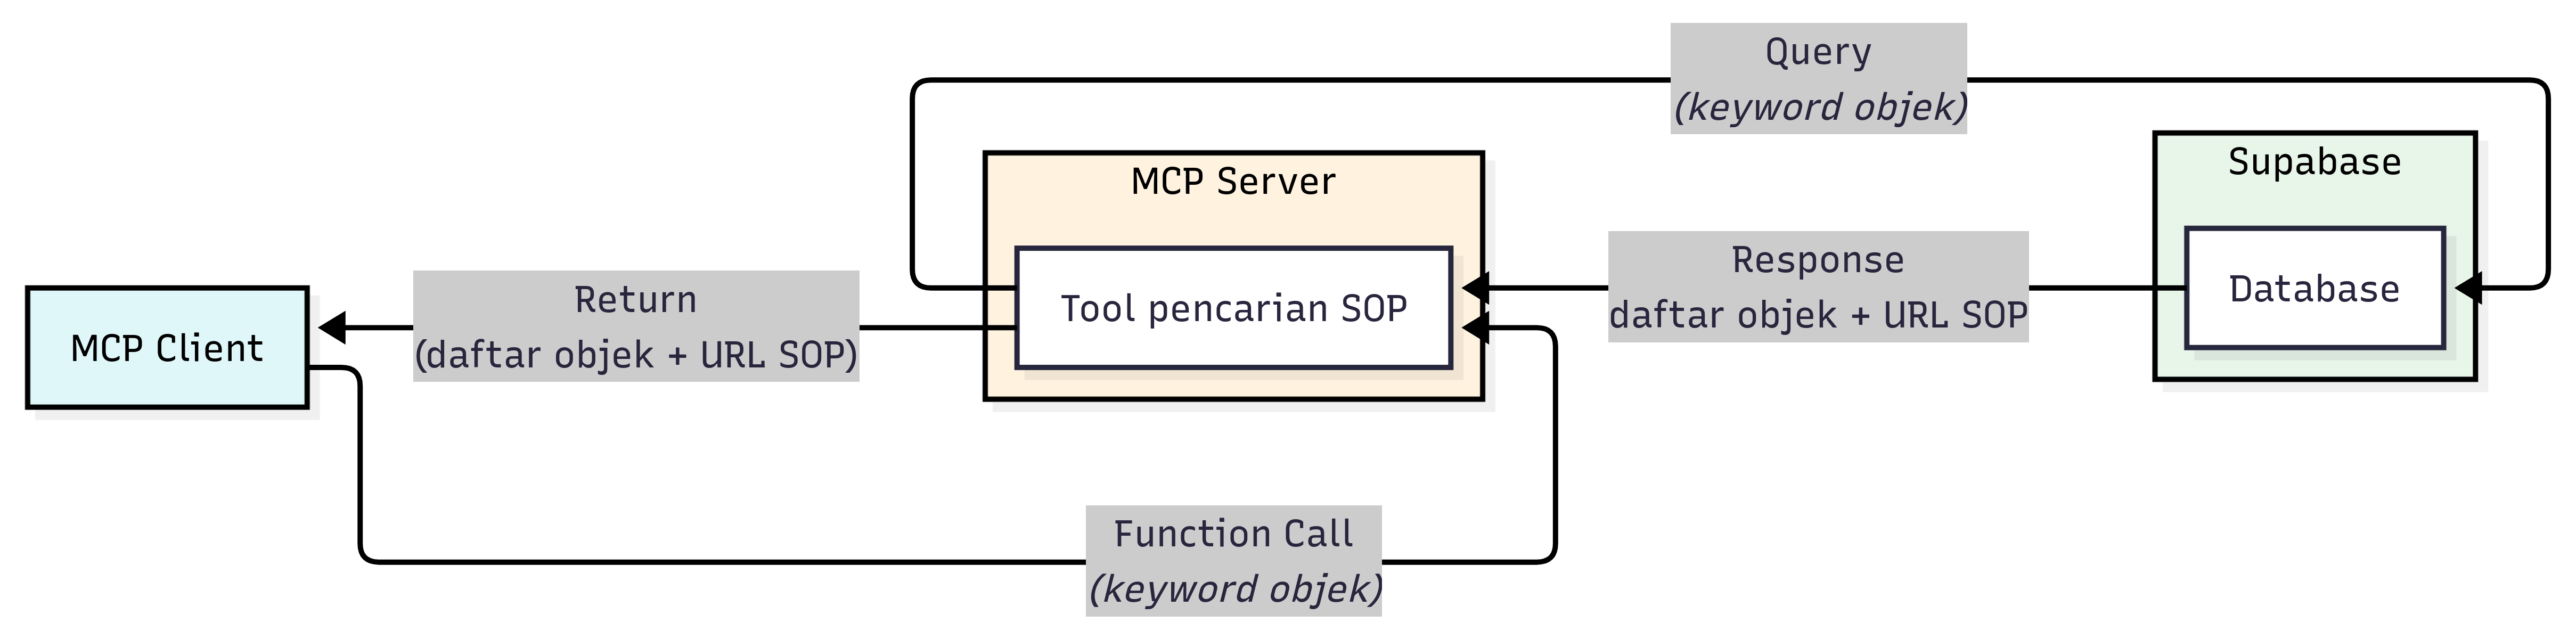
\includegraphics[width=1.0\textwidth]{Init/diagram-mcp-server/tool_sop.png}
    \caption{Diagram \textit{Tool} Pencarian Berkas SOP}
    \label{fig:diagram_tool_sop}
\footnotesize \textbf{Sumber:} Dokumentasi Penulis
\end{figure}
Seperti yang divisualisasikan pada Gambar \ref{fig:diagram_tool_sop}, \textit{tool} ini bertujuan untuk mencari  dokumen \textit{Standard Operating Procedure} (SOP) di dalam basis data. Agen AI cukup mengirimkan parameter masukan berupa nama objek atau kata kunci, lalu \textit{tool} ini akan melakukan pencarian kueri ke basis data dan mengembalikan daftar objek beserta tautan (\textit{URL}) berkas SOP yang berelasi dengannya. \textit{Tool} ini secara spesifik dirancang untuk hanya memberikan meta-informasi tanpa langsung mengekstrak isi teks dokumen guna menghemat penggunaan token pada jendela konteks model bahasa. Proses pengunduhan dokumen dari \textit{cloud storage} serta ekstraksi teks secara mendalam (baik dari format PDF maupun DOCX) akan dijalankan secara otomatis oleh MCP client di belakang layar.

\subsubsection{\textit{Tool} Pengambilan dan Analisis \textit{Image}}
\begin{figure}[H]
    \centering
    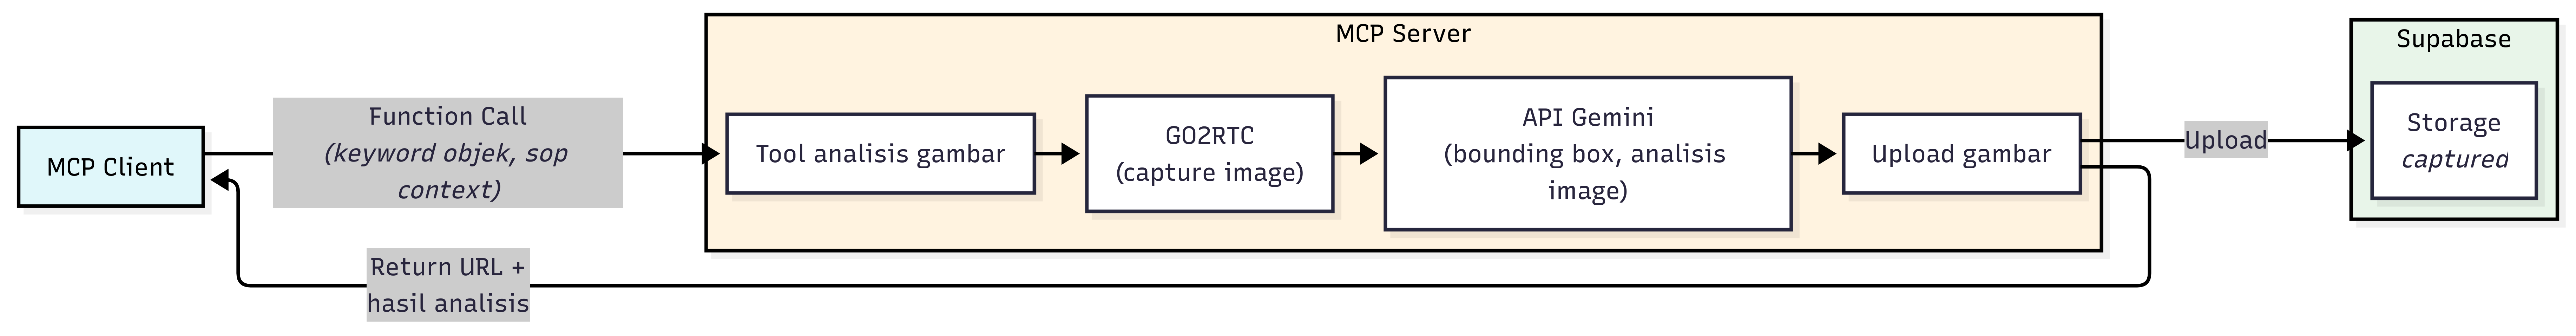
\includegraphics[width=1.0\textwidth]{Init/diagram-mcp-server/tool_analisis_image.png}
    \caption{Diagram \textit{Tool} Pengambilan dan Analisis \textit{Image}}
    \label{fig:diagram_tool_analisis}
\footnotesize \textbf{Sumber:} Dokumentasi Penulis
\end{figure}
Seperti yang ditunjukkan pada Gambar \ref{fig:diagram_tool_analisis}, \textit{tool} pengambilan dan analisis \textit{image} inspeksi merupakan \textit{tool} utama untuk mendeteksi objek serta menganalisis kondisinya. \textit{Tool} ini menerima parameter berupa kata kunci objek yang diperiksa. Pertama, server mengambil \textit{image} mentah dari kamera robot melalui protokol snapshot go2rtc. Jika objek yang diperiksa didefinisikan, \textit{image} tersebut dikirim ke model Gemini beserta teks instruksi deteksi objek. Model Gemini akan mengembalikan koordinat pembatas objek dalam bentuk bilangan bulat ternormalisasi. \textit{Image} mentah kemudian dipotong menggunakan modul OpenCV berdasarkan koordinat tersebut dengan menambahkan \textit{margin} sebesar 20 persen (\%) agar objek fokus di tengah. Jika teks prosedur standar disertakan, model Gemini akan menganalisis visual objek dan mengembalikan temuan inspeksi, analisis rinci, serta status kelayakan objek berupa normal, abnormal, atau tidak meyakinkan. \textit{Image} hasil pemrosesan kemudian diunggah ke penyimpanan Supabase dan server mengembalikan tautan publik beserta data analisis terstruktur kepada client.

\subsection{Sistem ROS}
Sistem perangkat lunak robot quadruped ini berjalan di atas Robot Operating System atau ROS dengan memanfaatkan repositori bawaan DeepRobotics yang dimodifikasi. Sistem ROS tersebut bertanggung jawab atas koordinasi sensor, navigasi, lokalisasi, pemetaan lingkungan sekitar, serta penerjemahan data telemetri.

\subsubsection{Lokalisasi dan Pemetaan SLAM} 
\begin{figure}[h!]
    \centering
    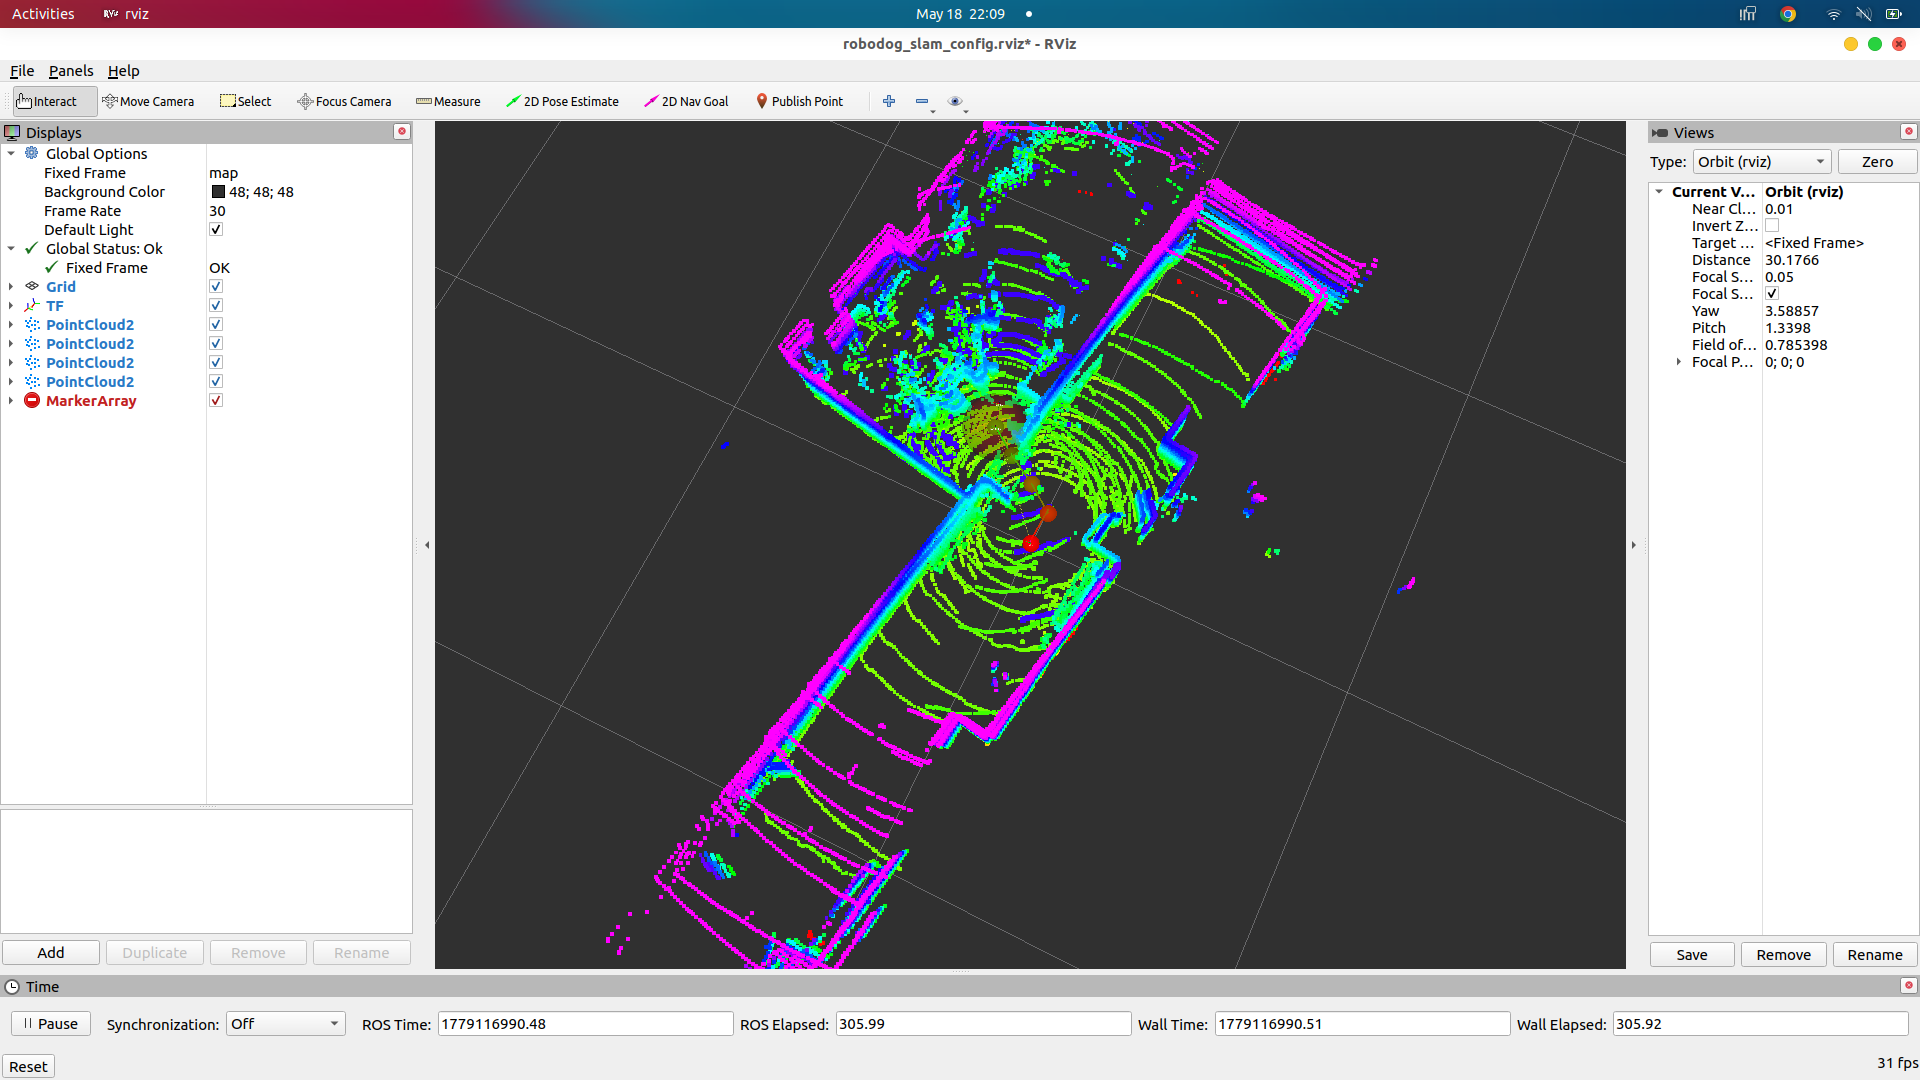
\includegraphics[width=1.0\textwidth]{Init/gambar/mapping.png}
    \caption{Proses pemetaan dan lokalisasi pada Robot}
    \label{fig:mapping}
\footnotesize \textbf{Sumber:} Dokumentasi Penulis
\end{figure}
Sebagaimana diilustrasikan pada diagram Gambar \ref{fig:mapping}, proses lokalisasi dan pemetaan lingkungan dilakukan dengan memanfaatkan algoritma pemetaan yang sudah tersedia pada sistem bawaan robot. Proses ini dijalankan dengan mengeksekusi \textit{executable file} pemetaan dari repositori bawaan yang secara otomatis bertugas menerima dan memproses data pindaian \textit{point cloud} tiga dimensi dari sensor LiDAR. Sistem pemetaan bawaan ini digunakan secara praktis tanpa melakukan perancangan algoritma pemetaan baru ataupun modifikasi pemrosesan tingkat rendah. Hasil akhir dari proses pemetaan ini berupa peta \textit{point cloud} tiga dimensi yang kemudian disimpan dan digunakan sebagai peta acuan utama navigasi bagi robot.

\subsubsection{Navigasi} 
\begin{figure}[H]
    \centering
    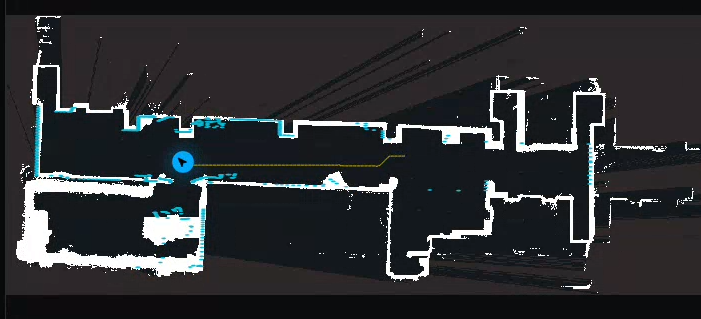
\includegraphics[width=1.0\textwidth]{Init/gambar/navigasi.png}
    \caption{Proses navigasi pada Robot}
    \label{fig:navigasi}
\footnotesize \textbf{Sumber:} Dokumentasi Penulis
\end{figure}
Proses navigasi otonom robot diaktifkan melalui antarmuka web operator dengan menekan tombol inisialisasi. Aksi ini akan memicu skrip inisialisasi navigasi pada komputer robot yang bertugas memuat peta lingkungan yang telah dibuat sebelumnya. Skrip ini meluncurkan komponen pencarian posisi lokal berbasis pencocokan pindaian LiDAR tiga dimensi yang dikombinasikan dengan data dari sensor inersia atau IMU. Hal tersebut memungkinkan robot mengetahui lokasinya secara presisi dalam koordinat peta tanpa harus bergantung pada sensor eksternal. Sistem navigasi ini menggunakan \textit{navigation stack} yang mengintegrasikan perencana jalur global untuk mencari rute terpendek dan perencana jalur lokal untuk menghindari rintangan dinamis secara real-time. Sebuah contoh dari proses navigasi robot menuju satu titik tujuan dapat dilihat pada Gambar \ref{fig:navigasi}.

\subsubsection{\textit{RosBridge WebSocket}}
\begin{figure}[H]
    \centering
    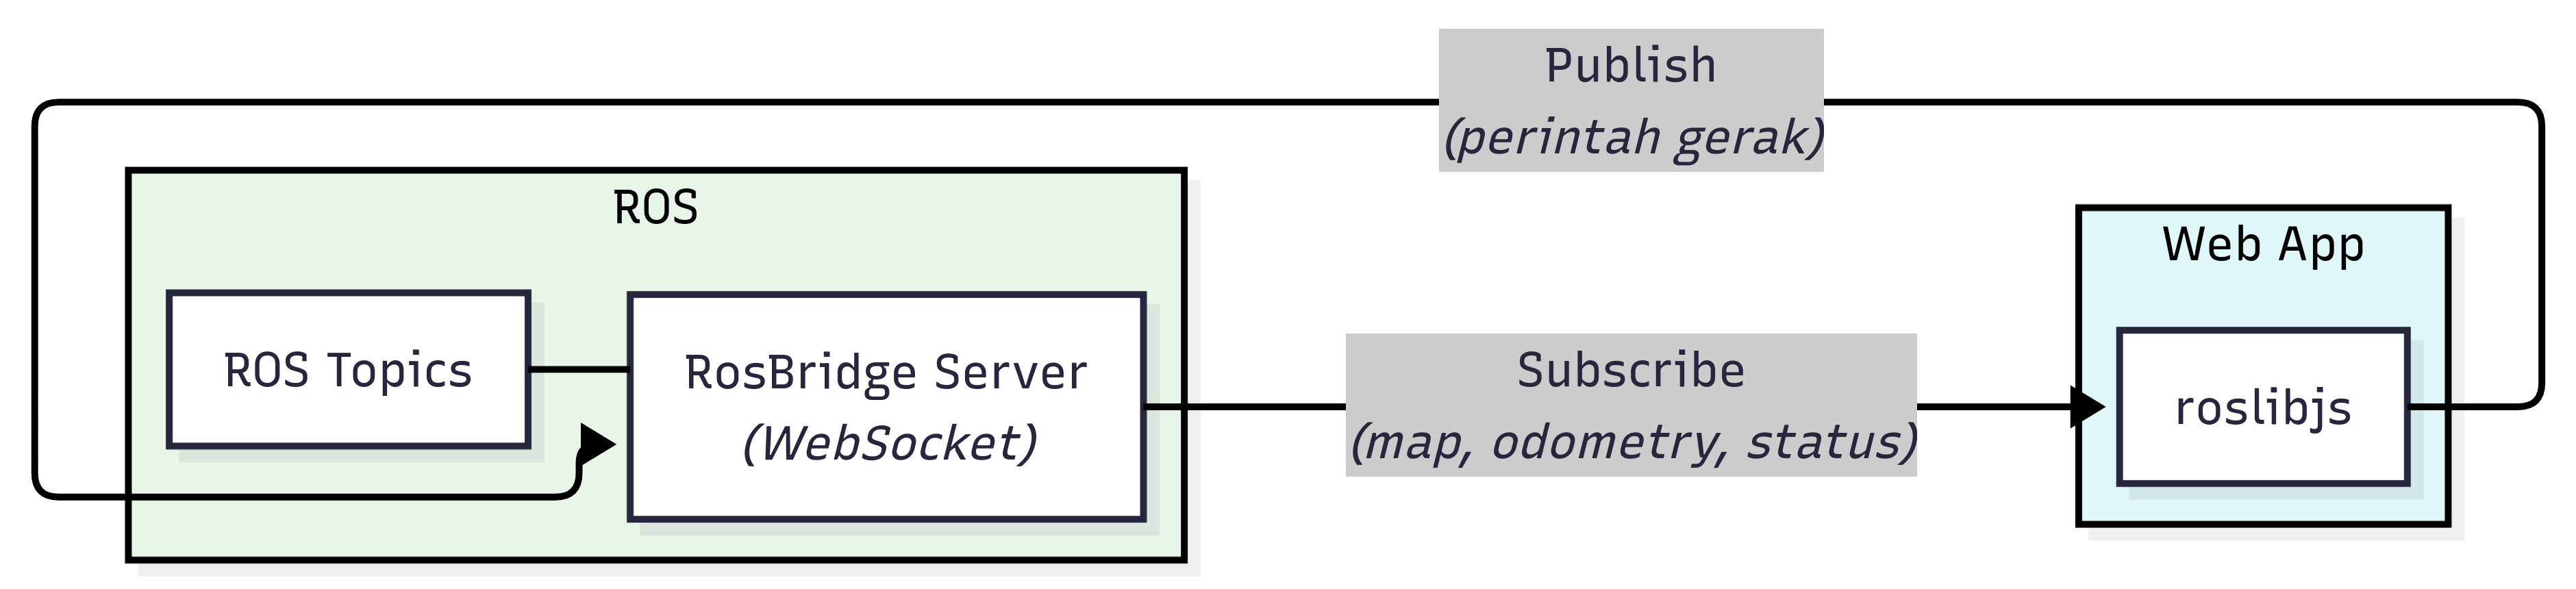
\includegraphics[width=0.8\textwidth]{Init/diagram-ros/rosbridge.png}
    \caption{Diagram \textit{RosBridge WebSocket}}
    \label{fig:diagram_rosbridge}
\footnotesize \textbf{Sumber:} Dokumentasi Penulis
\end{figure}
Seperti yang diilustrasikan pada Gambar \ref{fig:diagram_rosbridge}, komunikasi dua arah antara aplikasi antarmuka web dengan sistem ROS di dalam robot difasilitasi oleh modul \textit{rosbridge suite}. Modul ini menjalankan server WebSocket pada port 9090 di dalam komputer robot. Antarmuka web menggunakan pustaka \textit{roslibjs} untuk melakukan koneksi ke WebSocket tersebut, sehingga operator dapat mengirimkan perintah gerak, menerima data status robot, menerima data peta, serta data koordinat secara langsung. Penggunaan protokol ini sangat efisien karena data dipertukarkan dalam format teks JSON secara asinkron.

\subsubsection{ROS \textit{Messages Transformer}}
\begin{figure}[H]
    \centering
    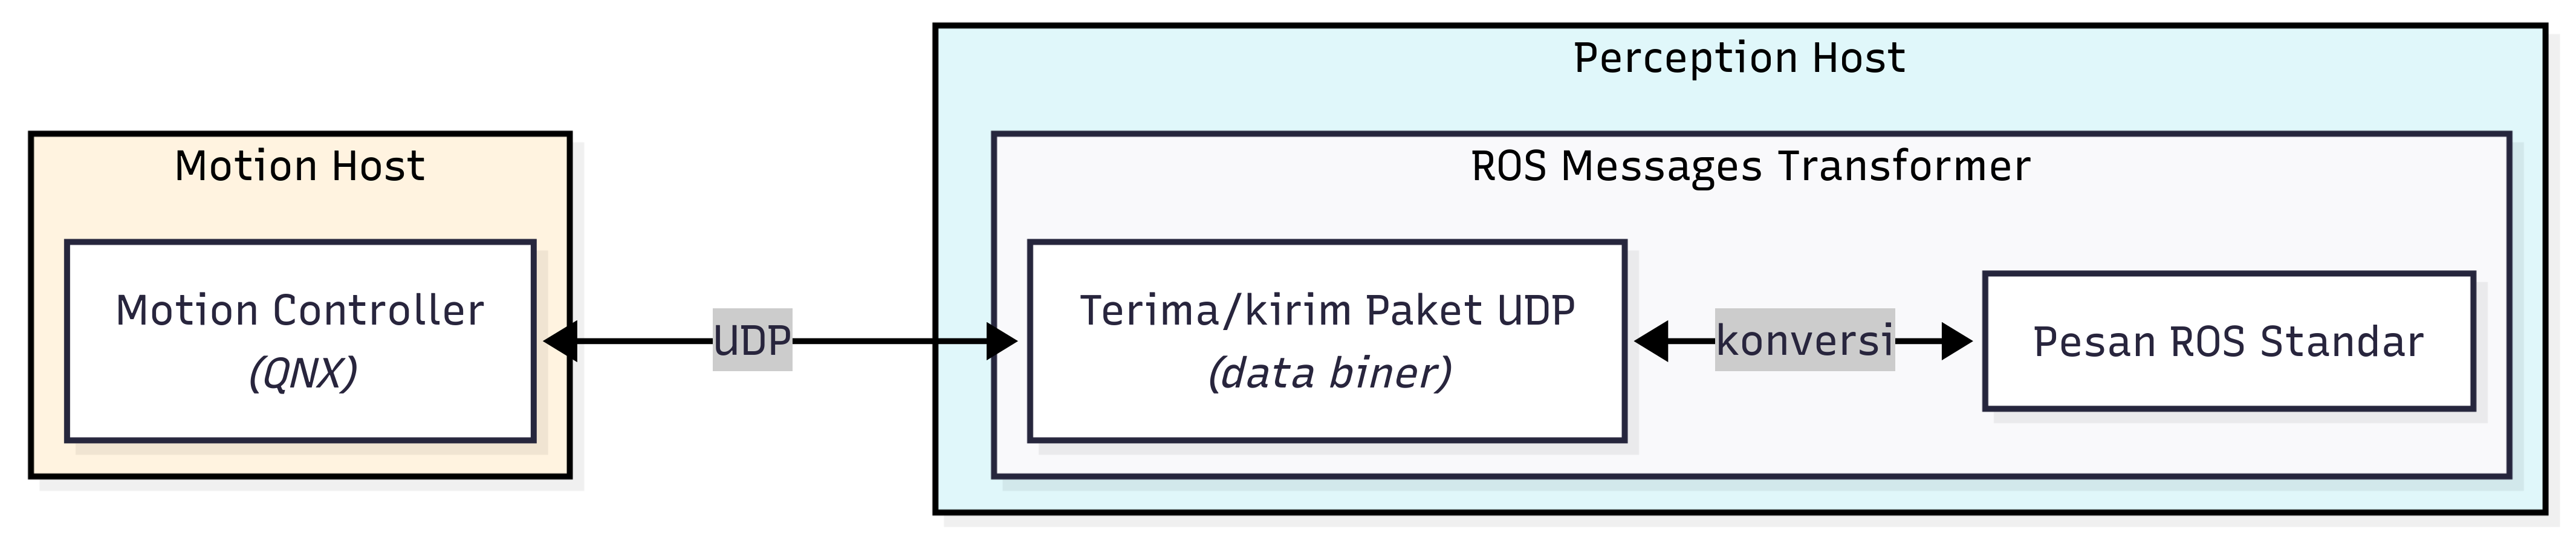
\includegraphics[width=0.8\textwidth]{Init/diagram-ros/msg_transformer.png}
    \caption{Diagram ROS \textit{Messages Transformer}}
    \label{fig:diagram_msg_transformer}
\footnotesize \textbf{Sumber:} Dokumentasi Penulis
\end{figure}
Seperti yang ditunjukkan pada Gambar \ref{fig:diagram_msg_transformer}, modul penerjemah pesan atau \textit{message transformer} digunakan untuk menjembatani komunikasi dua arah tingkat rendah antara sistem kendali gerak robot yang berjalan pada sistem operasi QNX di dalam \textit{Motion Host} dengan ekosistem ROS di \textit{Perception Host}. Pada arah masuk, modul ini menerima paket data biner melalui protokol UDP yang berisi parameter kecepatan motor, kondisi sendi, serta data sensor inersia dari \textit{Motion Controller}, kemudian mengemasnya kembali menjadi pesan ROS standar. Pada arah keluar, modul ini juga menerjemahkan perintah pergerakan dari topik ROS menjadi paket data biner UDP yang dikirimkan ke \textit{Motion Controller} untuk menggerakkan aktuator fisik robot. Untuk memenuhi kebutuhan pemantauan \textit{real-time} pada antarmuka web, modul ini dimodifikasi dengan menambahkan fungsionalitas ekstra berupa ekstraksi informasi kapasitas baterai dan status dasar robot. Data tersebut kemudian dipublikasikan ke dalam topik ROS /battery\_level dan /robot\_basic\_state yang memungkinkan data tersebut disalurkan melalui rosbridge ke aplikasi antarmuka pengguna.

\subsection{Implementasi Basis Data}
\begin{figure}[h!]
    \centering
    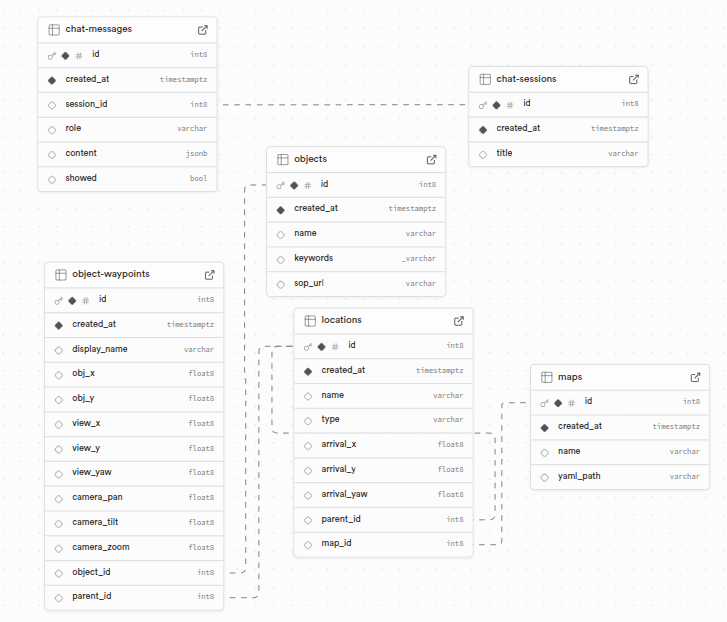
\includegraphics[width=1.0\textwidth]{Init/gambar/database.png}
    \caption{ERD Supabase}
    \label{fig:ERD}
\footnotesize \textbf{Sumber:} Dokumentasi Penulis
\end{figure}
Sistem ini menggunakan Supabase sebagai penyedia layanan basis data relasional berbasis PostgreSQL. Basis data ini dirancang untuk menyimpan data spasial lingkungan kerja robot, informasi koordinat objek inspeksi, berkas prosedur operasi standar, serta seluruh riwayat percakapan antara operator dan agen AI. Hubungan antartabel di dalam basis data dirancang secara relasional untuk menjamin konsistensi data koordinat serta memudahkan proses kueri yang dilakukan oleh server. Hubungan relasional antartabel basis data ini dapat dilihat pada Gambar \ref{fig:ERD}.

\subsubsection{Tabel \textit{Maps}}
Tabel maps berfungsi untuk menyimpan metadata peta lingkungan dua dimensi maupun tiga dimensi yang telah dihasilkan oleh robot. Tabel ini memiliki kolom id sebagai \textit{primary key} dengan tipe data bilangan bulat yang bersifat inkremental. Kolom created\_at mencatat waktu pembuatan data dengan tipe stempel waktu beserta zona waktu. Kolom name bertipe karakter digunakan untuk menyimpan nama peta yang mudah dipahami manusia. Kolom yaml\_path bertipe karakter menyimpan alamat jalur penyimpanan berkas konfigurasi peta pada sistem robot. Tabel ini memiliki relasi \textit{one-to-many} dengan tabel lokasi. Di dalam sistem, data peta ini diakses oleh aplikasi antarmuka web Next.js saat operator memilih profil peta awal sesi, serta digunakan oleh skrip inisialisasi navigasi untuk memuat berkas konfigurasi peta acuan.

\subsubsection{Tabel \textit{Locations}}
Tabel locations dirancang untuk memodelkan struktur hierarki lokasi fisik di dalam area kerja robot, seperti gedung, lantai, atau ruangan tertentu. Tabel ini memiliki kolom id sebagai \textit{primary key}. Kolom created\_at mencatat waktu pembuatan data. Kolom name menyimpan nama lokasi dan kolom type menentukan kategori lokasi seperti ruangan atau lantai. Kolom arrival\_x, arrival\_y, dan arrival\_yaw bertipe angka desimal digunakan untuk menyimpan koordinat tujuan kedatangan robot saat memasuki lokasi tersebut. Kolom parent\_id merupakan \textit{foreign key} yang merujuk kembali ke kolom \textit{primary key} tabel ini sendiri untuk membentuk hubungan hierarkis bertingkat. Kolom map\_id merupakan \textit{foreign key} yang merujuk ke tabel peta untuk mengaitkan lokasi dengan peta acuan yang digunakan. Tabel ini digunakan oleh halaman navigasi spasial pada antarmuka web untuk menampilkan struktur lokasi, serta dibaca oleh MCP server untuk mendapatkan peta semantik.

\subsubsection{Tabel \textit{Objects}}
Tabel objects menyimpan daftar tipe objek fisik yang menjadi target inspeksi oleh robot. Tabel ini memiliki kolom id sebagai \textit{primary key} dan kolom created\_at untuk stempel waktu. Kolom name digunakan untuk menyimpan nama jenis objek inspeksi. Kolom keywords bertipe \textit{array} teks digunakan oleh agen AI untuk mencocokkan nama objek yang ditanyakan oleh operator. Kolom sop\_url bertipe karakter menyimpan tautan menuju berkas prosedur standar inspeksi objek tersebut. Tabel ini dibaca oleh \textit{tool} pencari koordinat objek pada MCP Server saat melakukan pencocokan kata kunci objek yang dikirim oleh agen AI.

\subsubsection{Tabel \textit{Object Waypoints}}
Tabel object-waypoints berfungsi untuk menghubungkan objek inspeksi dengan koordinat objek. Tabel ini memiliki kolom id sebagai \textit{primary key} dan kolom created\_at untuk stempel waktu. Kolom display\_name menyimpan nama titik inspeksi. Kolom obj\_x dan obj\_y menyimpan estimasi koordinat lokasi objek itu sendiri. Kolom view\_x, view\_y, dan view\_yaw menyimpan koordinat navigasi yang harus dicapai robot untuk dapat melihat objek dengan baik. Kolom camera\_pan, camera\_tilt, dan camera\_zoom menyimpan parameter konfigurasi sudut kamera agar mengarah tepat ke objek. Kolom object\_id bertipe \textit{foreign key} yang merujuk ke tabel objek, sedangkan kolom parent\_id bertipe \textit{foreign key} yang merujuk ke tabel lokasi. Data dari tabel ini digunakan oleh \textit{tool} pencari koordinat objek pada MCP Server untuk mendapatkan target koordinat navigasi yang dikirimkan ke stack navigasi ROS.

\subsubsection{Tabel \textit{Chat Sessions}}
Tabel chat-sessions digunakan untuk mencatat setiap sesi percakapan baru yang diinisialisasi oleh operator melalui antarmuka pengguna. Tabel ini memiliki kolom id sebagai \textit{primary key}. Kolom created\_at mencatat stempel waktu inisialisasi sesi. Kolom title bertipe karakter digunakan untuk menyimpan judul sesi percakapan guna memudahkan pencarian riwayat oleh operator. Tabel ini memiliki relasi \textit{one-to-many} dengan tabel pesan percakapan. Tabel ini diakses oleh MCP client untuk membuat sesi baru dan menampilkan daftar sesi percakapan yang telah ada pada antarmuka web.

\subsubsection{Tabel \textit{Chat Messages}}
Tabel chat-messages berfungsi untuk menyimpan seluruh riwayat pesan di dalam setiap sesi percakapan secara terperinci. Tabel ini memiliki kolom id sebagai \textit{primary key} dan kolom created\_at sebagai stempel waktu pengiriman pesan. Kolom session\_id bertipe \textit{foreign key} yang merujuk ke tabel sesi percakapan untuk mengelompokkan pesan. Kolom role bertipe karakter menentukan pengirim pesan, seperti pengguna, asisten model, atau sistem \textit{tool}. Kolom content bertipe format data JSON digunakan untuk menyimpan teks percakapan. Kolom showed bertipe boolean dengan nilai bawaan benar digunakan untuk mengontrol apakah pesan tersebut harus ditampilkan di halaman antarmuka pengguna atau hanya dibaca sebagai riwayat konteks oleh agen AI. Tabel ini terhubung erat dengan antarmuka percakapan web yang menampilkan pesan secara dinamis. Modul MCP client menulis pesan baru ke tabel ini, dan perubahan data langsung memicu pembaruan pada tampilan antarmuka web secara real-time. Web juga membaca tabel ini untuk menampilkan percakapan saat ini dan memuat riwayat percakapan lama ketika operator memilih sesi tertentu.

\subsubsection{Supabase \textit{Storage}}
Selain tabel relasional, sistem ini menggunakan Supabase Storage sebagai wadah penyimpanan berkas objek tidak terstruktur. Penyimpanan ini dibagi menjadi dua folder utama. Folder pertama yaitu folder prosedur standar yang bertugas menyimpan dokumen panduan inspeksi objek dalam format dokumen. Folder ini dibaca oleh \textit{tool} pencari dokumen prosedur pada MCP Server untuk mengunduh dokumen panduan inspeksi. Folder kedua yaitu folder \textit{image} hasil tangkapan yang berfungsi untuk menyimpan foto mentah dari kamera robot serta foto hasil pemotongan fokus objek inspeksi. Setiap berkas yang diunggah ke dalam folder \textit{image} akan menghasilkan alamat tautan publik yang nantinya disimpan pada kolom konten di tabel pesan percakapan agar dapat ditampilkan langsung ke layar operator. Folder ini diakses oleh \textit{tool} pengambilan \textit{image} pada MCP Server untuk menyimpan \textit{image}. Storage ini juga digunakan oleh MCP Client untuk mengunduh berkas dokumen SOP dan \textit{image} hasil inspeksi agar dapat disisipkan kembali ke dalam konteks percakapan model bahasa Gemini. Web juga membaca storage ini untuk menampilkan \textit{image} dan dokumen SOP pada halaman terkait.
\cleardoublepage
\chapter{PENGUJIAN}
\label{sec:chap4_pengujian}
\vspace{1ex}

\section{Rancangan Pengujian}
\label{sec:deskripsi_pengujian}

Pengujian dilakukan secara bertahap untuk mengevaluasi kinerja setiap komponen fungsional utama maupun sistem secara keseluruhan. Sebagaimana ditetapkan pada rumusan tujuan penelitian, sistem yang dikembangkan memiliki dua tujuan utama. Tujuan pertama adalah mengintegrasikan \textit{Multimodal Large Language Model} untuk menggerakkan robot menggunakan bahasa alami serta melakukan analisis visual otomatis berbasis dokumen SOP. Tujuan kedua adalah mengembangkan arsitektur kendali \textit{Human-in-the-Loop}  dengan metode eksekusi rencana bertahap. Oleh karena itu, rangkaian pengujian dirancang untuk memverifikasi pencapaian kedua tujuan tersebut secara terstruktur. Seluruh pengujian fungsional dilakukan pada tiga model MLLM yang berbeda, yaitu Gemini 3.1 Pro Preview, Gemini 2.5 Flash, dan Qwen 3.5 27B.

Pemilihan ketiga model tersebut didasarkan pada pertimbangan sebagai berikut. Gemini 3.1 Pro Preview dipilih sebagai representasi model berskala besar dengan kemampuan penalaran tingkat tinggi yang merupakan salah satu model terbaik dari Gemini. Gemini 2.5 Flash dipilih karena merupakan model tercepat dan termurah yang masih tersedia, sehingga cocok digunakan sebagai \textit{baseline} pembanding yang adil terhadap Qwen 3.5 yang juga beroperasi pada kelas efisiensi serupa. Pemilihan Qwen 3.5 27B sendiri dilatarbelakangi oleh pertimbangan \textit{future-proofing}, mengingat pengaplikasian robot inspeksi di lingkungan nyata akan lebih optimal jika menggunakan model lokal karena dapat menghilangkan biaya langganan API serta meminimalkan latensi jaringan. Meskipun pada implementasi ini Qwen masih dijalankan pada server terpisah dan belum tertanam langsung di dalam robot, pengujian ini bertujuan untuk mengukur kelayakan model lokal sebagai alternatif pengganti model berbasis \textit{cloud} di masa mendatang.

Pengujian terdiri dari lima kategori utama. Tiga pengujian pertama, yaitu pengujian pemanggilan \textit{tools}, pengujian analisis objek, dan pengujian pembuatan \textit{plan}, mengevaluasi kompo\-nen-kompo\-nen inti yang mendukung tujuan pertama, yaitu kemampuan MLLM dalam memahami instruksi bahasa alami, menganalisis kondisi visual objek, dan menyusun rencana inspeksi secara otonom. Pengujian keempat berupa pengujian keseluruhan sistem secara \textit{end-to-end} mengevaluasi integrasi seluruh komponen sekaligus memverifikasi tujuan kedua, yaitu keberhasilan mekanisme eksekusi bertahap dan kemampuan sistem dalam menangani intervensi operator di tengah misi. Pengujian kelima menggunakan kuesioner NASA-TLX untuk mengukur dampak sistem terhadap beban kerja operator secara kuantitatif, yang menjadi indikator keberhasilan akhir dari kedua tujuan penelitian.

% =============================================================================
% PENGUJIAN 1: PEMANGGILAN TOOLS
% =============================================================================
\section{Pengujian Pemanggilan \textit{Tools}}
\label{sec:pengujian_tools}

Pengujian ini bertujuan untuk mengevaluasi kemampuan setiap model MLLM dalam memahami instruksi operator dan memetakannya ke pemanggilan \textit{tools} yang tepat beserta parameter yang sesuai. Kemampuan ini merupakan fondasi utama dari seluruh sistem, karena seluruh aksi fisik robot dieksekusi melalui mekanisme \textit{function calling} pada Model Context Protocol.

\subsection{Skenario Pengujian}
Dataset pengujian terdiri dari 72 kasus uji yang mencakup 8 jenis \textit{tool} yang tersedia dalam sistem, yaitu async\_move, async\_navigate\_to\_waypoint, capture\_and\_inspect\_image, get\_object\_waypoints, get\_sop\_file, look\_up\_down, say\_hello, dan toggle\_sit\_stand. Setiap jenis \textit{tool} diuji pada tiga level kesulitan instruksi sebagai berikut:

\begin{enumerate}
    \item \textbf{Level 1 (Eksplisit)}: Instruksi menyebutkan nama \textit{tool} dan parameter secara langsung dan jelas, misalnya \textit{``Gerakkan robot maju dengan kecepatan linear 0,5 m/s selama 3 detik.''}
    \item \textbf{Level 2 (Semi-Implisit)}: Instruksi menggunakan bahasa alami yang merujuk pada fungsi tertentu tanpa menyebutkan nama \textit{tool} secara eksplisit, misalnya \textit{``Maju pelan-pelan ke depan sekitar 3 detik.''}
    \item \textbf{Level 3 (Abstrak)}: Instruksi diberikan secara kontekstual dan memerlukan penalaran semantik untuk menentukan \textit{tool} dan parameter yang tepat, misalnya \textit{``Posisimu terlalu dekat dengan dinding, geser sedikit.''}
\end{enumerate}

Masing-masing kombinasi \textit{tool} dan level diuji sebanyak 3 kali pertanyaan berbeda, sehingga total terdapat $8 \times 3 \times 3 = 72$ kasus uji per model. Setiap kasus uji dievaluasi berdasarkan keberhasilan pemanggilan \textit{tool} yang benar, rata-rata latensi respons dalam detik, dan rata-rata konsumsi total token.

\subsection{Hasil Pengujian}

% --- Tabel Ringkasan Keseluruhan ---
\begin{table}[H]
\centering
\caption{Ringkasan Hasil Pengujian Pemanggilan \textit{Tools}}
\label{tab:tools_summary}
\begin{tabular}{|l|c|c|c|}
\hline
\textbf{Metrik} & \textbf{Gemini 2.5 Flash} & \textbf{Gemini 3.1 Pro} & \textbf{Qwen 3.5 27B} \\
\hline
Persentase Keberhasilan & 93,06\% & 98,61\% & 88,89\% \\
\hline
Rata-rata Latensi (detik) & 2,03 & 4,11 & 2,96 \\
\hline
Rata-rata Total Token & 1.139 & 1.144 & 1.587 \\
\hline
\end{tabular}
\end{table}

% --- Tabel Detail Per Tool Per Level ---
\begin{longtable}{|l|c|c|c|c|c|c|c|c|c|}
\caption{Detail Hasil Pengujian Pemanggilan \textit{Tools} per Jenis \textit{Tool} dan Level} \label{tab:tools_detail} \\
\hline
\multirow{2}{*}{\textbf{Jenis Tool}} & \multirow{2}{*}{\textbf{Level}} & \multicolumn{2}{c|}{\textbf{Gemini 2.5 Flash}} & \multicolumn{2}{c|}{\textbf{Gemini 3.1 Pro}} & \multicolumn{2}{c|}{\textbf{Qwen 3.5 27B}} \\
\cline{3-8}
& & \textbf{Skor} & \textbf{Latensi} & \textbf{Skor} & \textbf{Latensi} & \textbf{Skor} & \textbf{Latensi} \\
\hline
\endfirsthead
\hline
\multirow{2}{*}{\textbf{Jenis Tool}} & \multirow{2}{*}{\textbf{Level}} & \multicolumn{2}{c|}{\textbf{Gemini 2.5 Flash}} & \multicolumn{2}{c|}{\textbf{Gemini 3.1 Pro}} & \multicolumn{2}{c|}{\textbf{Qwen 3.5 27B}} \\
\cline{3-8}
& & \textbf{Skor} & \textbf{Latensi} & \textbf{Skor} & \textbf{Latensi} & \textbf{Skor} & \textbf{Latensi} \\
\hline
\endhead
async\_move & L1 & 3/3 & 1,54 & 3/3 & 3,58 & 3/3 & 3,40 \\
\hline
async\_move & L2 & 3/3 & 1,68 & 3/3 & 4,12 & 3/3 & 3,00 \\
\hline
async\_move & L3 & 3/3 & 1,65 & 3/3 & 4,55 & 2/3 & 5,06 \\
\hline
async\_navigate & L1 & 3/3 & 1,60 & 3/3 & 4,52 & 3/3 & 3,76 \\
\hline
async\_navigate & L2 & 3/3 & 2,04 & 3/3 & 4,12 & 3/3 & 3,41 \\
\hline
async\_navigate & L3 & 3/3 & 1,84 & 3/3 & 3,76 & 3/3 & 3,80 \\
\hline
capture\_inspect & L1 & 3/3 & 1,74 & 3/3 & 9,26 & 3/3 & 2,73 \\
\hline
capture\_inspect & L2 & 3/3 & 2,05 & 3/3 & 4,12 & 1/3 & 3,43 \\
\hline
capture\_inspect & L3 & 3/3 & 1,93 & 3/3 & 5,12 & 3/3 & 4,04 \\
\hline
get\_object\_wp & L1 & 3/3 & 1,43 & 3/3 & 3,00 & 3/3 & 2,72 \\
\hline
get\_object\_wp & L2 & 3/3 & 1,69 & 3/3 & 3,93 & 3/3 & 4,39 \\
\hline
get\_object\_wp & L3 & 3/3 & 1,83 & 3/3 & 4,25 & 3/3 & 3,34 \\
\hline
get\_sop\_file & L1 & 3/3 & 1,64 & 3/3 & 2,68 & 3/3 & 1,94 \\
\hline
get\_sop\_file & L2 & 3/3 & 2,01 & 3/3 & 2,96 & 3/3 & 2,14 \\
\hline
get\_sop\_file & L3 & 3/3 & 1,86 & 3/3 & 4,24 & 3/3 & 2,44 \\
\hline
look\_up\_down & L1 & 3/3 & 1,51 & 3/3 & 3,80 & 3/3 & 2,01 \\
\hline
look\_up\_down & L2 & 3/3 & 3,66 & 3/3 & 6,57 & 3/3 & 2,17 \\
\hline
look\_up\_down & L3 & 0/3 & 2,68 & 2/3 & 7,36 & 1/3 & 2,23 \\
\hline
say\_hello & L1 & 3/3 & 1,46 & 3/3 & 3,14 & 3/3 & 3,46 \\
\hline
say\_hello & L2 & 3/3 & 1,25 & 3/3 & 2,86 & 3/3 & 1,83 \\
\hline
say\_hello & L3 & 3/3 & 1,76 & 3/3 & 5,84 & 2/3 & 2,95 \\
\hline
toggle\_sit\_stand & L1 & 3/3 & 1,57 & 3/3 & 3,05 & 3/3 & 2,15 \\
\hline
toggle\_sit\_stand & L2 & 3/3 & 1,53 & 3/3 & 2,92 & 3/3 & 2,00 \\
\hline
toggle\_sit\_stand & L3 & 1/3 & 1,70 & 3/3 & 3,69 & 1/3 & 2,74 \\
\hline
\end{longtable}

\begin{figure}[H]
    \centering
    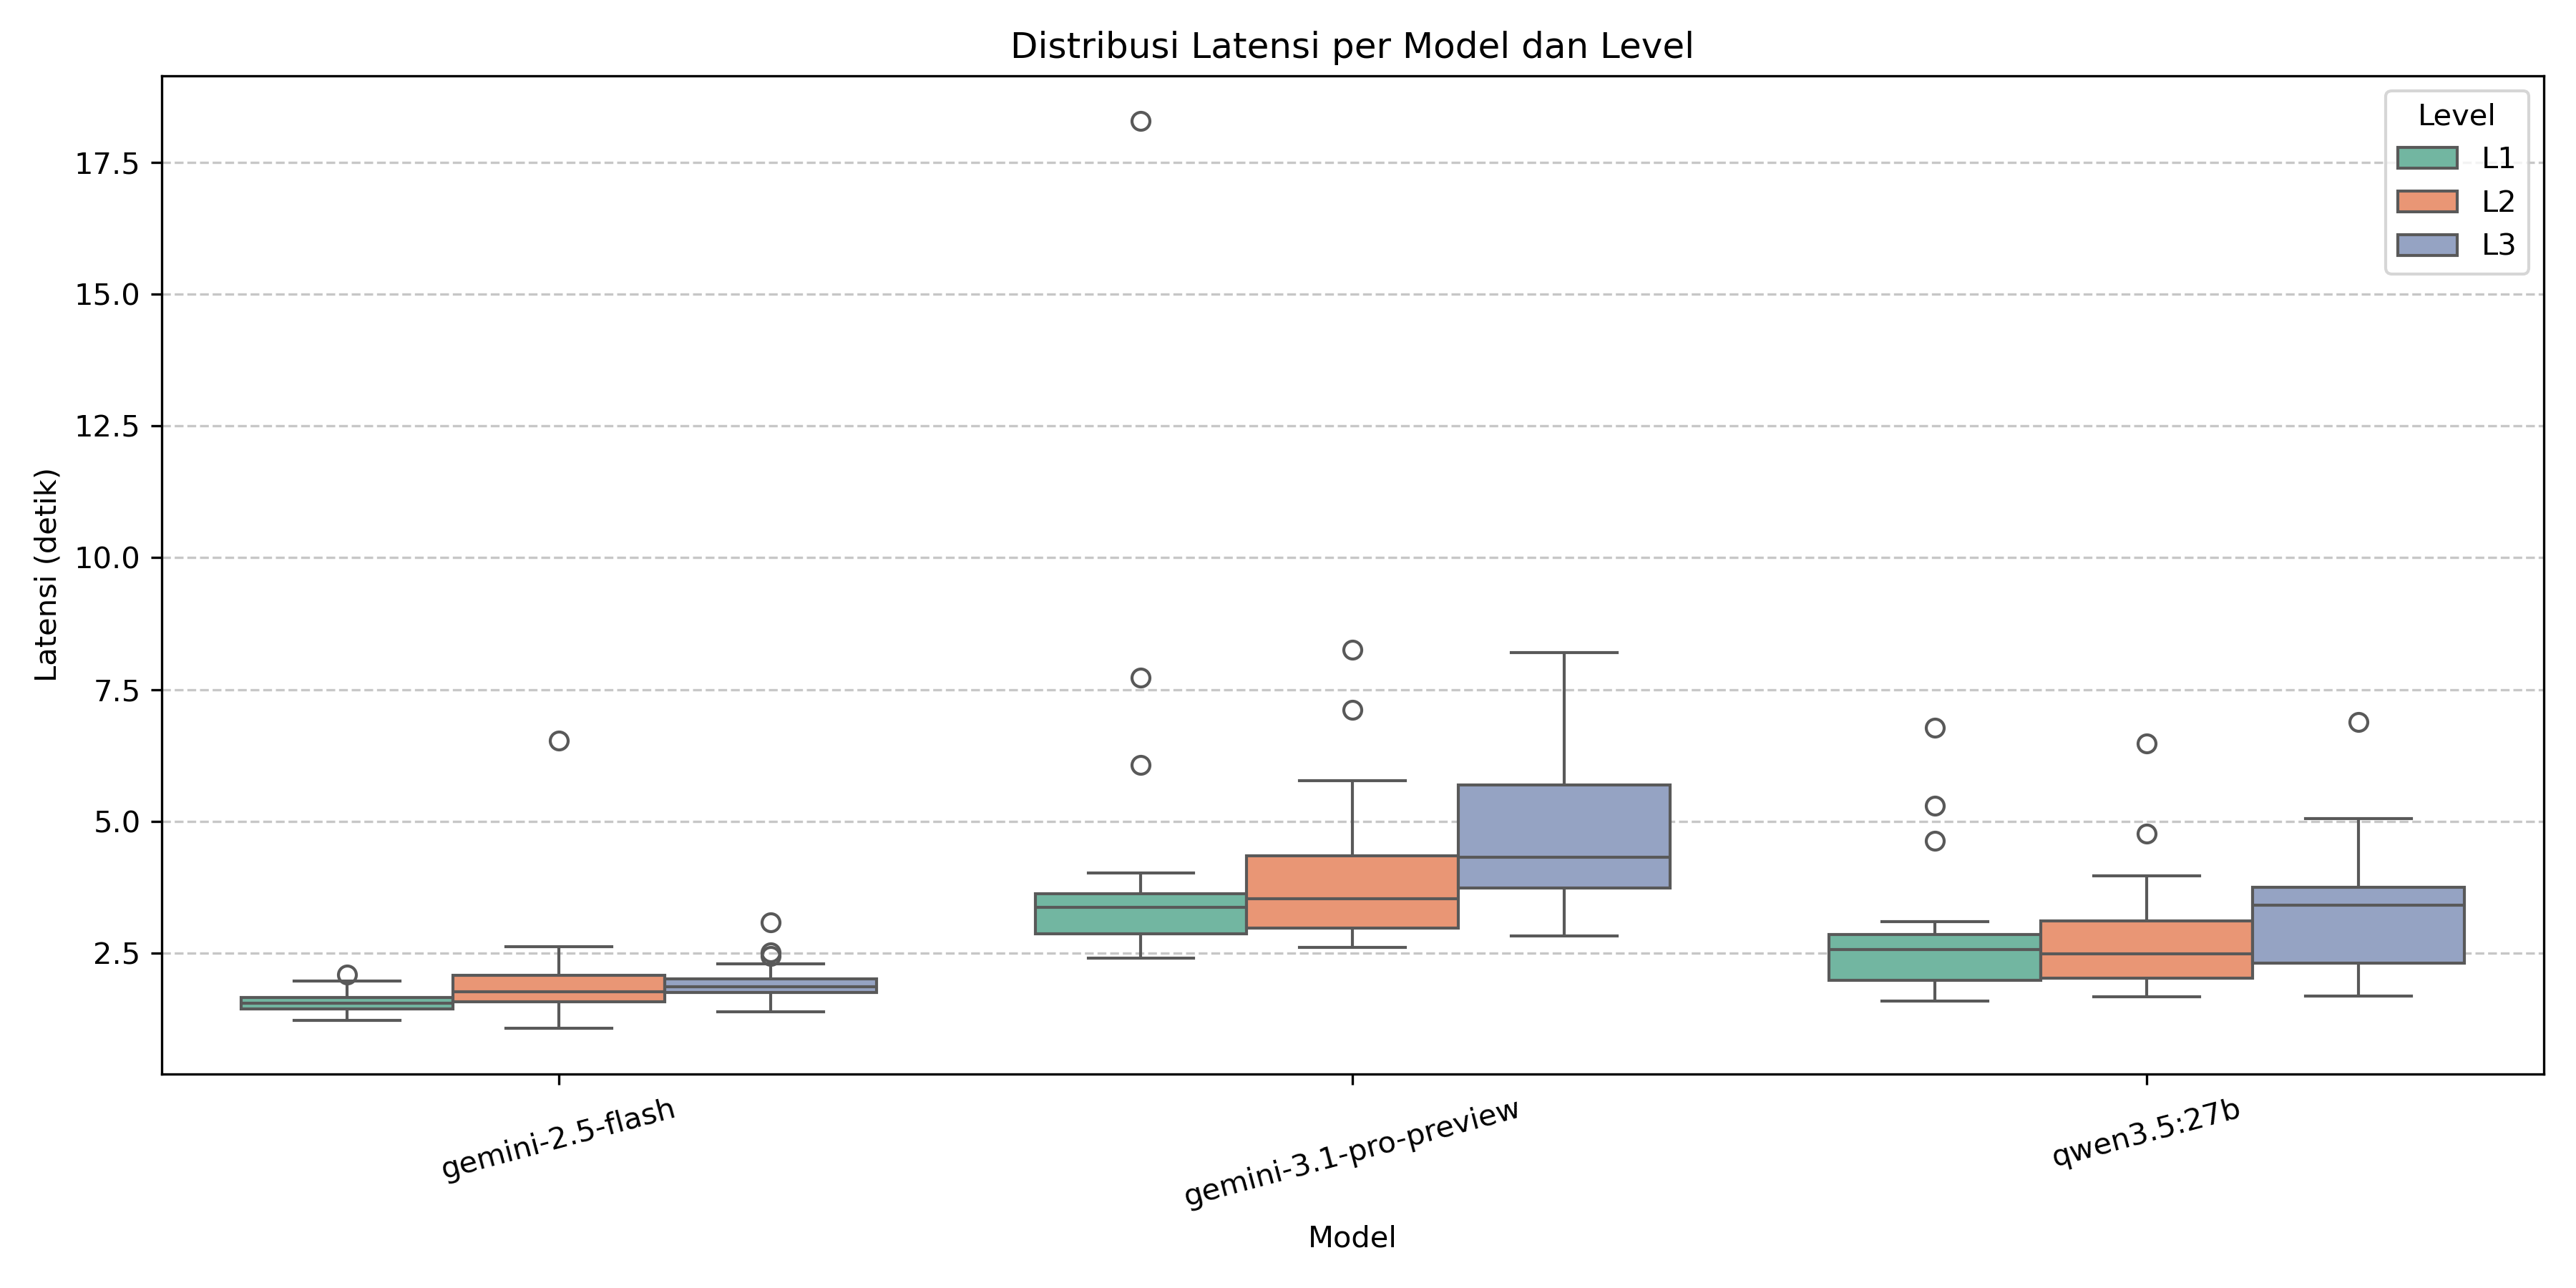
\includegraphics[width=0.8\textwidth]{Init/gambar/boxplots/boxplot_tools_latensi.png}
    \caption{Distribusi Latensi Pengujian Pemanggilan \textit{Tools} per Model}
    \label{fig:boxplot_tools_latensi}
\footnotesize \textbf{Sumber:} Dokumentasi Penulis
\end{figure}

\begin{figure}[H]
    \centering
    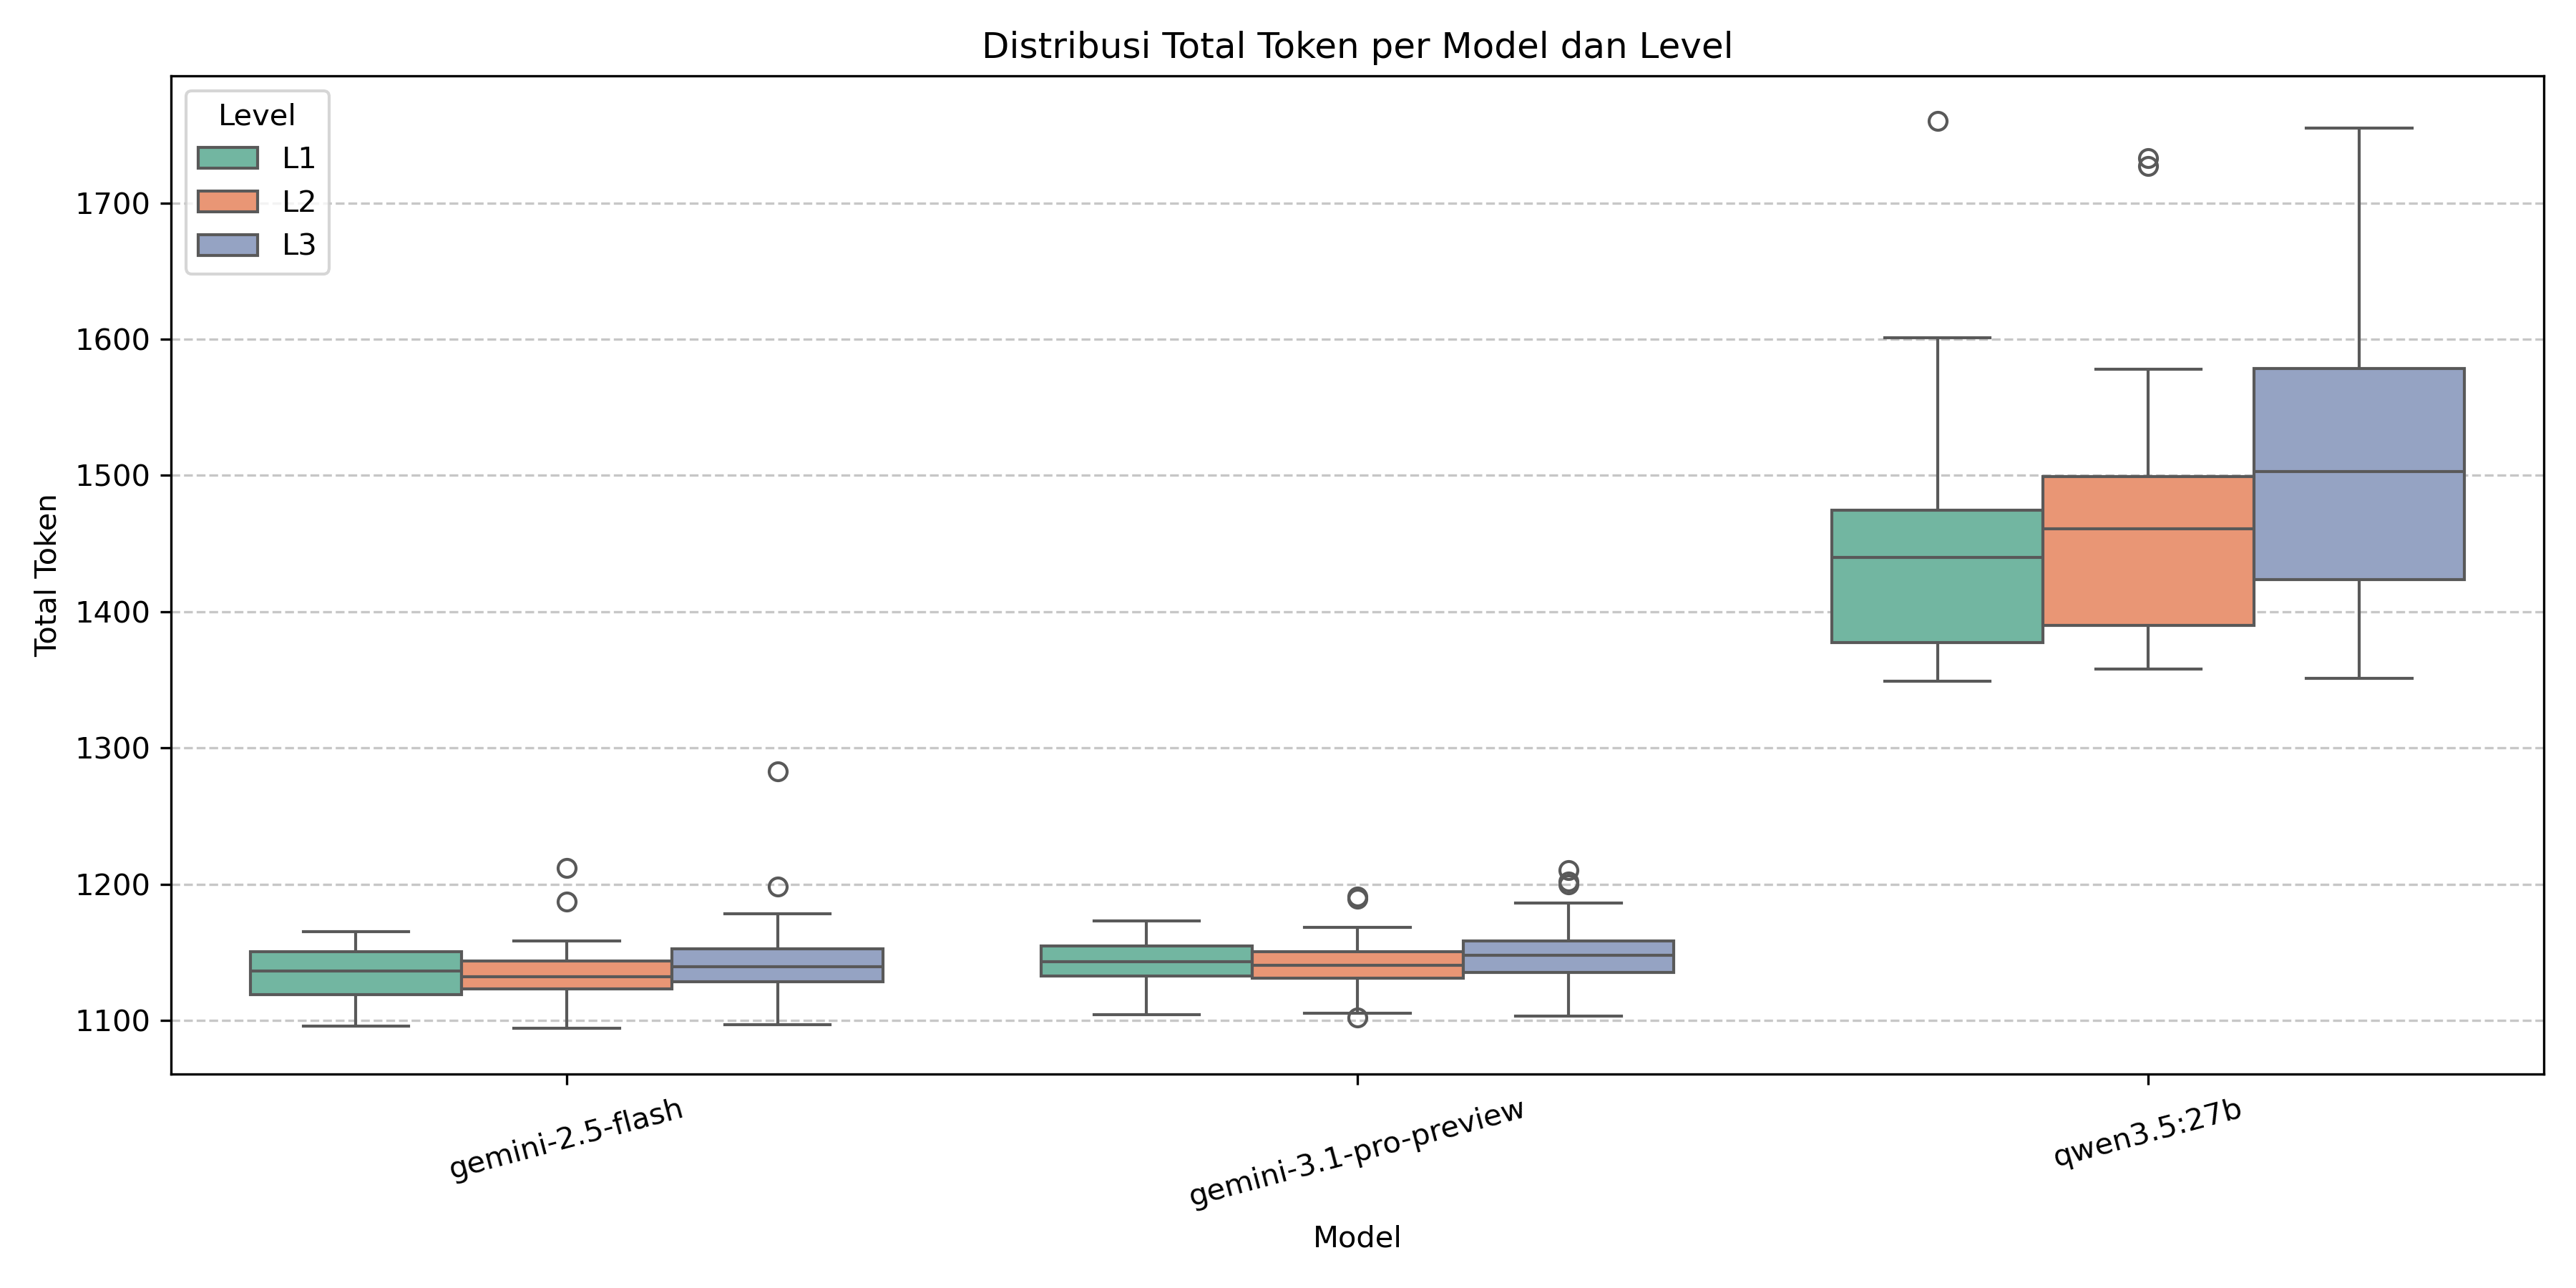
\includegraphics[width=0.8\textwidth]{Init/gambar/boxplots/boxplot_tools_token.png}
    \caption{Distribusi Konsumsi Token Pengujian Pemanggilan \textit{Tools} per Model}
    \label{fig:boxplot_tools_token}
\footnotesize \textbf{Sumber:} Dokumentasi Penulis
\end{figure}

\subsection{Analisis Data Keberhasilan}
Berdasarkan hasil pengujian pada Tabel \ref{tab:tools_summary} dan Tabel \ref{tab:tools_detail}, Gemini 3.1 Pro Preview mencatatkan persentase keberhasilan tertinggi sebesar 98,61\%, diikuti oleh Gemini 2.5 Flash sebesar 93,06\%, dan Qwen 3.5 27B sebesar 88,89\%. Ketiga model menunjukkan performa sempurna pada Level 1 dan Level 2 untuk mayoritas \textit{tools}, dengan seluruh kegagalan terkonsentrasi pada Level 3. Pola ini menunjukkan bahwa ketiga model telah menguasai pemetaan instruksi eksplisit ke \textit{function calling} dengan baik, namun menghadapi tantangan yang berbeda-beda saat instruksi memerlukan penalaran kontekstual yang tinggi. Tiga \textit{tool} yang menjadi sumber kegagalan utama pada Level 3 adalah look\_up\_down, say\_hello, dan toggle\_sit\_stand. Ketiganya memiliki kesamaan karakteristik, yaitu instruksi Level 3 yang diberikan tidak menyebutkan aksi robot secara langsung melainkan mendeskripsikan situasi atau konteks yang mengharuskan model menyimpulkan tindakan yang tepat secara mandiri.

Berdasarkan hasil pengujian, beberapa pola kegagalan pemanggilan \textit{tool} berhasil diidentifikasi. Pada pengujian Gemini 2.5 Flash terhadap \textit{tool} look\_up\_down serta Qwen 3.5 terhadap \textit{tool} say\_hello, model mampu memahami konteks yang diberikan pengguna, namun tidak melakukan pemanggilan \textit{tool}. Model lebih memilih memberikan konfirmasi atau menjelaskan tindakan yang akan dilakukan daripada langsung mengeksekusi \textit{tool}. Pola ini menunjukkan adanya kecenderungan model untuk meminta konfirmasi meskipun konteks yang diberikan telah cukup untuk menentukan aksi yang sesuai. Pada pengujian Gemini 2.5 Flash dan Qwen 3.5 terhadap \textit{tool} toggle\_sit\_stand, model bahkan gagal mengenali maksud instruksi sebagai perintah untuk mengubah postur robot, sehingga respons yang dihasilkan tidak mengarah pada pemanggilan \textit{tool} maupun aksi yang sesuai. Hal ini menunjukkan bahwa model belum mampu menghubungkan makna instruksi dengan \textit{tool} yang tersedia. Model hanya memahami makna literal dari kalimat, tetapi gagal mengidentifikasi bahwa percakapan tersebut merupakan perintah yang seharusnya memicu perubahan postur robot. Karakteristik kegagalan yang berbeda ditemukan pada pengujian Gemini 3.1 Pro dan Qwen 3.5 terhadap \textit{tool} look\_up\_down, serta Qwen 3.5 terhadap \textit{tool} capture\_and\_inspect\_image. Pada kasus ini, model cenderung melakukan \textit{planning} berlebihan sebelum menjalankan \textit{tool}. Alih-alih langsung mengeksekusi \textit{tool} yang diperlukan, model terlebih dahulu berusaha melengkapi informasi lain yang berkaitan dengan proses inspeksi. Akibatnya, pemanggilan \textit{tool} yang sebenarnya sudah dapat dilakukan berdasarkan konteks yang tersedia menjadi tidak dilakukan. Sementara itu, pada pengujian Qwen 3.5 terhadap \textit{tool} async\_move, ditemukan kesalahan dalam pemilihan \textit{tool}. Model memilih \textit{tool} yang memiliki fungsi berbeda dengan aksi yang dimaksud oleh pengguna. Hal ini menunjukkan adanya kegagalan dalam memetakan makna bahasa alami ke fungsi \textit{tool} yang sesuai.

Secara keseluruhan, analisis ini membuktikan bahwa instruksi yang bersifat abstrak dan multi-interpretasi pada Level 3 merupakan tantangan utama bagi agen MLLM. Model dengan ukuran parameter besar seperti Gemini 3.1 Pro mampu menalar konteks spasial dan situasional dengan lebih baik, meskipun sempat gagal karena melakukan \textit{planning} berlebihan. Di sisi lain, model yang lebih kecil atau dioptimasi untuk kecepatan, seperti Gemini 2.5 Flash dan Qwen 3.5 27B, cenderung lebih rentan terhadap kegagalan dalam penalaran intruksi abstrak, Baik dalam bentuk kegagalan memicu tool, sehingga model hanya memberikan respons tekstual, maupun kesalahan dalam pemilihan tool yang tepat.


\subsection{Analisis Latensi dan Konsumsi \textit{Token}}
Berdasarkan distribusi latensi (Gambar \ref{fig:boxplot_tools_latensi}) dan konsumsi token (Gambar \ref{fig:boxplot_tools_token}), terlihat tren yang konsisten terhadap kompleksitas level instruksi dan karakteristik model. Secara umum, Gemini 2.5 Flash memiliki waktu respons paling singkat pada seluruh level pengujian, menunjukkan performa yang lebih baik dari sisi latensi dibandingkan model lainnya. Qwen 3.5 berada di posisi menengah, sementara Gemini 3.1 Pro mencatatkan latensi tertinggi akibat kecenderungannya melakukan proses penalaran yang lebih kompleks. Peningkatan latensi yang sejalan dengan naiknya level kesulitan instruksi menunjukkan bahwa kompleksitas \textit{prompt} berdampak langsung pada waktu pemrosesan model. Dari sisi konsumsi token, kedua varian Gemini memiliki penggunaan yang stabil dan identik di seluruh level karena berbagi arsitektur \textit{tokenizer} yang sama. Sebaliknya, Qwen 3.5 mengonsumsi token jauh lebih besar dengan rentang yang lebar akibat model ini sering memberikan respons tekstual yang panjang. Temuan ini membuktikan bahwa jumlah token tidak selalu berbanding lurus dengan waktu respons, tingginya latensi Gemini 3.1 Pro bersumber dari mekanisme penalaran internal (\textit{reasoning}), bukan sekadar panjang keluaran.

% =============================================================================
% PENGUJIAN 2: ANALISIS OBJEK
% =============================================================================
\section{Pengujian Analisis Objek}
\label{sec:pengujian_inspeksi}
Pengujian ini bertujuan untuk mengevaluasi kemampuan model MLLM dalam menganalisis kondisi fisik objek inspeksi melalui \textit{image} yang ditangkap oleh kamera robot. Evaluasi dilakukan dengan membandingkan hasil analisis model terhadap kondisi aktual objek berdasarkan dokumen \textit{Standard Operating Procedure} yang relevan.

\subsection{Skenario Pengujian}
Pengujian dilakukan terhadap tiga jenis objek target inspeksi, yaitu APAR, stop kontak, dan tong sampah. Setiap objek diuji dalam tiga kondisi yang berbeda sebagai berikut:

\begin{table}[H]
\centering
\caption{Skenario Kondisi Pengujian Analisis Objek (APAR dan Stop Kontak)}
\label{tab:skenario_analisis_objek_1}
\renewcommand{\arraystretch}{1.5}
\resizebox{\linewidth}{!}{
\begin{tabular}{|l|l|p{5cm}|c|}
\hline
\textbf{Objek} & \textbf{Tipe Kondisi} & \textbf{Deskripsi} & \textbf{Contoh \textit{Image}} \\
\hline
\multirow{3}{*}{APAR} & Normal & APAR terpasang sesuai prosedur & 
\begin{minipage}{3.5cm} \vspace{2mm} \centering 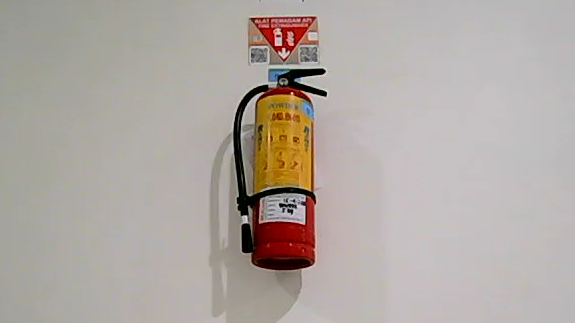
\includegraphics[height=2cm]{Init/gambar/image_uji/apar/normal/1781265608506.png} \vspace{2mm} \end{minipage} \\
\cline{2-4}
& Anomali 1 & APAR tergeletak di lantai & 
\begin{minipage}{3.5cm} \vspace{2mm} \centering 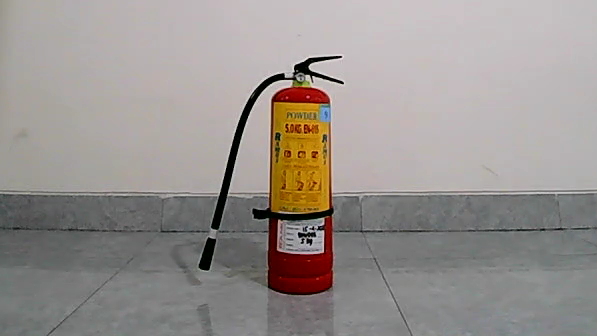
\includegraphics[height=2cm]{Init/gambar/image_uji/apar/tergeletak/1781265760647.png} \vspace{2mm} \end{minipage} \\
\cline{2-4}
& Anomali 2 & Selang tidak menempel pada klip \textit{body} & 
\begin{minipage}{3.5cm} \vspace{2mm} \centering 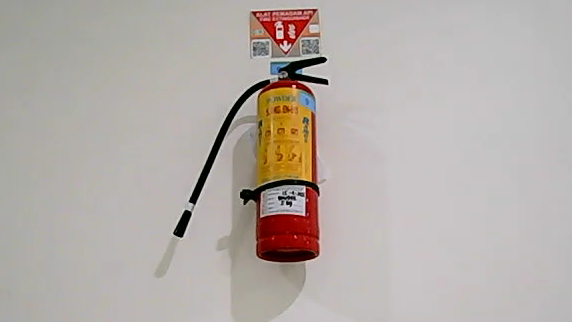
\includegraphics[height=2cm]{Init/gambar/image_uji/apar/selang_lepas/1781265701773.png} \vspace{2mm} \end{minipage} \\
\hline
\multirow{3}{*}{Stop Kontak} & Normal & Stop kontak dalam kondisi baik & 
\begin{minipage}{3.5cm} \vspace{2mm} \centering 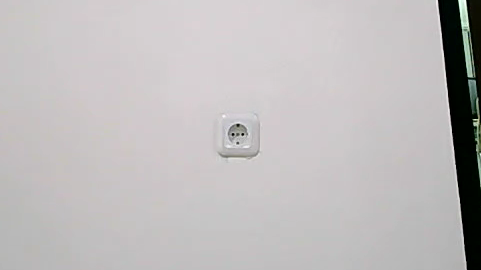
\includegraphics[height=2cm]{Init/gambar/image_uji/stop_kontak/normal/1781266626664.png} \vspace{2mm} \end{minipage} \\
\cline{2-4}
& Kondisi 1 & Terdapat steker normal yang terpasang & 
\begin{minipage}{3.5cm} \vspace{2mm} \centering 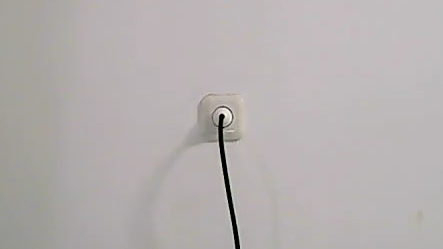
\includegraphics[height=2cm]{Init/gambar/image_uji/stop_kontak/tercolok_steker/1781266432749.png} \vspace{2mm} \end{minipage} \\
\cline{2-4}
& Anomali & Steker dengan kabel putus/rusak & 
\begin{minipage}{3.5cm} \vspace{2mm} \centering 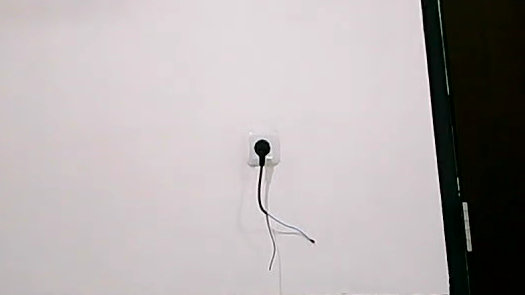
\includegraphics[height=2cm]{Init/gambar/image_uji/stop_kontak/steker_rusak/1781266701947.png} \vspace{2mm} \end{minipage} \\
\hline
\end{tabular}
}
\end{table}

\begin{table}[H]
\centering
\caption{Skenario Kondisi Pengujian Analisis Objek (Tong Sampah)}
\label{tab:skenario_analisis_objek_2}
\renewcommand{\arraystretch}{1.5}
\resizebox{\linewidth}{!}{
\begin{tabular}{|l|l|p{5cm}|c|}
\hline
\textbf{Objek} & \textbf{Tipe Kondisi} & \textbf{Deskripsi} & \textbf{Contoh Gambar} \\
\hline
\multirow{3}{*}{Tong Sampah} & Normal & Tiga tong sampah tersusun rapi & 
\begin{minipage}{3.5cm} \vspace{2mm} \centering 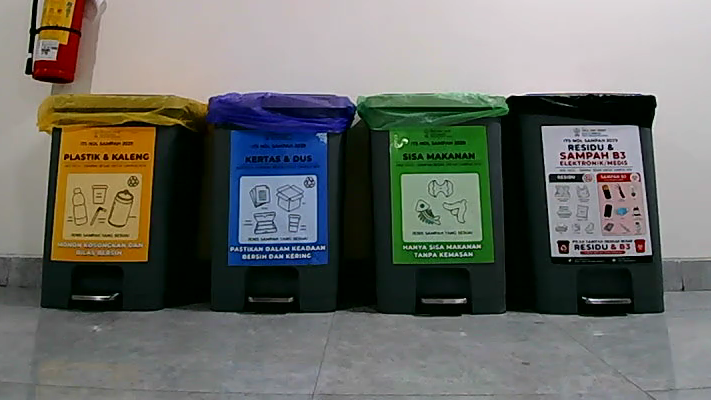
\includegraphics[height=2cm]{Init/gambar/image_uji/tong_sampah/normal/1781265874120.png} \vspace{2mm} \end{minipage} \\
\cline{2-4}
& Anomali 1 & Hanya terdapat dua tong sampah (tidak lengkap) & 
\begin{minipage}{3.5cm} \vspace{2mm} \centering 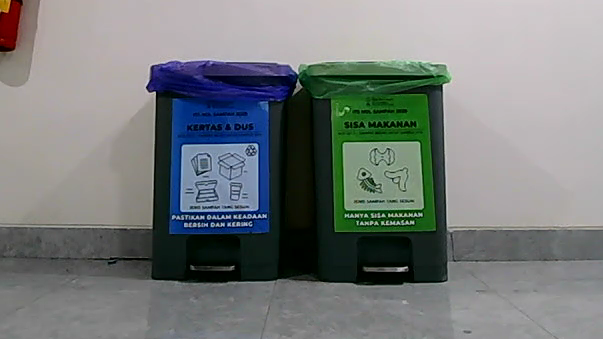
\includegraphics[height=2cm]{Init/gambar/image_uji/tong_sampah/tong_kurang/1781265905093.png} \vspace{2mm} \end{minipage} \\
\cline{2-4}
& Anomali 2 & Tong sampah berantakan dengan sampah berserakan & 
\begin{minipage}{3.5cm} \vspace{2mm} \centering 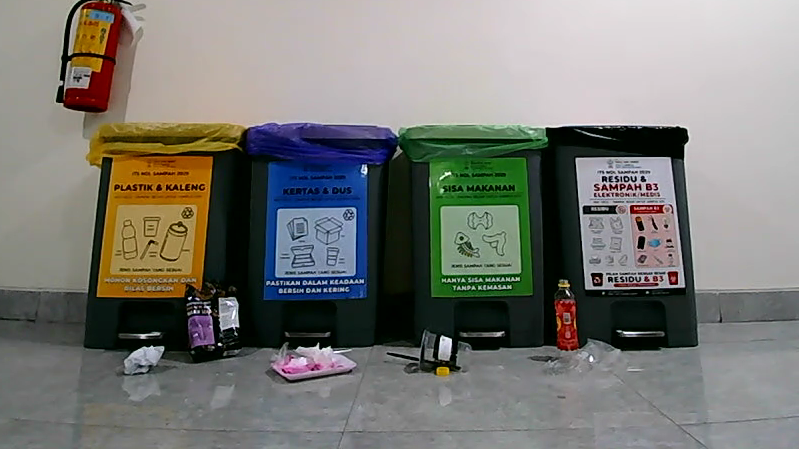
\includegraphics[height=2cm]{Init/gambar/image_uji/tong_sampah/sampah_berserakan/1781266320437.png} \vspace{2mm} \end{minipage} \\
\hline
\end{tabular}
}
\end{table}

Setiap kondisi diuji sebanyak tiga kali dari sudut pengambilan \textit{image} yang berbeda-beda untuk menguji konsistensi analisis model terhadap variasi sudut pandang kamera robot. Total terdapat $3 \times 3 \times 3 = 27$ kasus uji per model.

\subsection{Hasil Pengujian}

\begin{table}[H]
\centering
\caption{Ringkasan Hasil Pengujian Analisis Objek}
\label{tab:inspect_summary}
\begin{tabular}{|l|c|c|c|}
\hline
\textbf{Metrik} & \textbf{Gemini 2.5 Flash} & \textbf{Gemini 3.1 Pro} & \textbf{Qwen 3.5 27B} \\
\hline
Persentase Keberhasilan & 85,19\% & 100,00\% & 85,19\% \\
\hline
Rata-rata Latensi (detik) & 9,62 & 19,31 & 35,29 \\
\hline
Rata-rata Total Token & 1.980 & 3.297 & 5.071 \\
\hline
\end{tabular}
\end{table}

% --- Tabel Detail Per Objek Per Kondisi ---
\begin{longtable}{|l|l|c|c|c|c|c|c|}
\caption{Detail Hasil Pengujian Analisis Objek per Kondisi} \label{tab:inspect_detail} \\
\hline
\multirow{2}{*}{\textbf{Objek}} & \multirow{2}{*}{\textbf{Kondisi}} & \multicolumn{2}{c|}{\textbf{Gemini 2.5 Flash}} & \multicolumn{2}{c|}{\textbf{Gemini 3.1 Pro}} & \multicolumn{2}{c|}{\textbf{Qwen 3.5 27B}} \\
\cline{3-8}
& & \textbf{Skor} & \textbf{Latensi} & \textbf{Skor} & \textbf{Latensi} & \textbf{Skor} & \textbf{Latensi} \\
\hline
\endfirsthead
\hline
\multirow{2}{*}{\textbf{Objek}} & \multirow{2}{*}{\textbf{Kondisi}} & \multicolumn{2}{c|}{\textbf{Gemini 2.5 Flash}} & \multicolumn{2}{c|}{\textbf{Gemini 3.1 Pro}} & \multicolumn{2}{c|}{\textbf{Qwen 3.5 27B}} \\
\cline{3-8}
& & \textbf{Skor} & \textbf{Latensi} & \textbf{Skor} & \textbf{Latensi} & \textbf{Skor} & \textbf{Latensi} \\
\hline
\endhead
APAR & Tergeletak di lantai & 3/3 & 8,88 & 3/3 & 19,91 & 3/3 & 36,64 \\
\hline
APAR & Selang tidak menempel & 0/3 & 8,22 & 3/3 & 20,32 & 1/3 & 47,83 \\
\hline
APAR & Normal & 3/3 & 11,38 & 3/3 & 21,68 & 2/3 & 38,34 \\
\hline
Stop Kontak & Steker kabel putus & 2/3 & 9,02 & 3/3 & 17,68 & 2/3 & 27,13 \\
\hline
Stop Kontak & Normal & 3/3 & 7,82 & 3/3 & 15,32 & 3/3 & 23,43 \\
\hline
Stop Kontak & Steker normal & 3/3 & 8,98 & 3/3 & 15,45 & 3/3 & 32,98 \\
\hline
Tong Sampah & Hanya dua tong & 3/3 & 9,35 & 3/3 & 19,51 & 3/3 & 36,94 \\
\hline
Tong Sampah & Normal & 3/3 & 11,31 & 3/3 & 22,72 & 3/3 & 41,96 \\
\hline
Tong Sampah & Sampah berserakan & 3/3 & 11,65 & 3/3 & 21,19 & 3/3 & 32,38 \\
\hline
\end{longtable}

\begin{figure}[H]
    \centering
    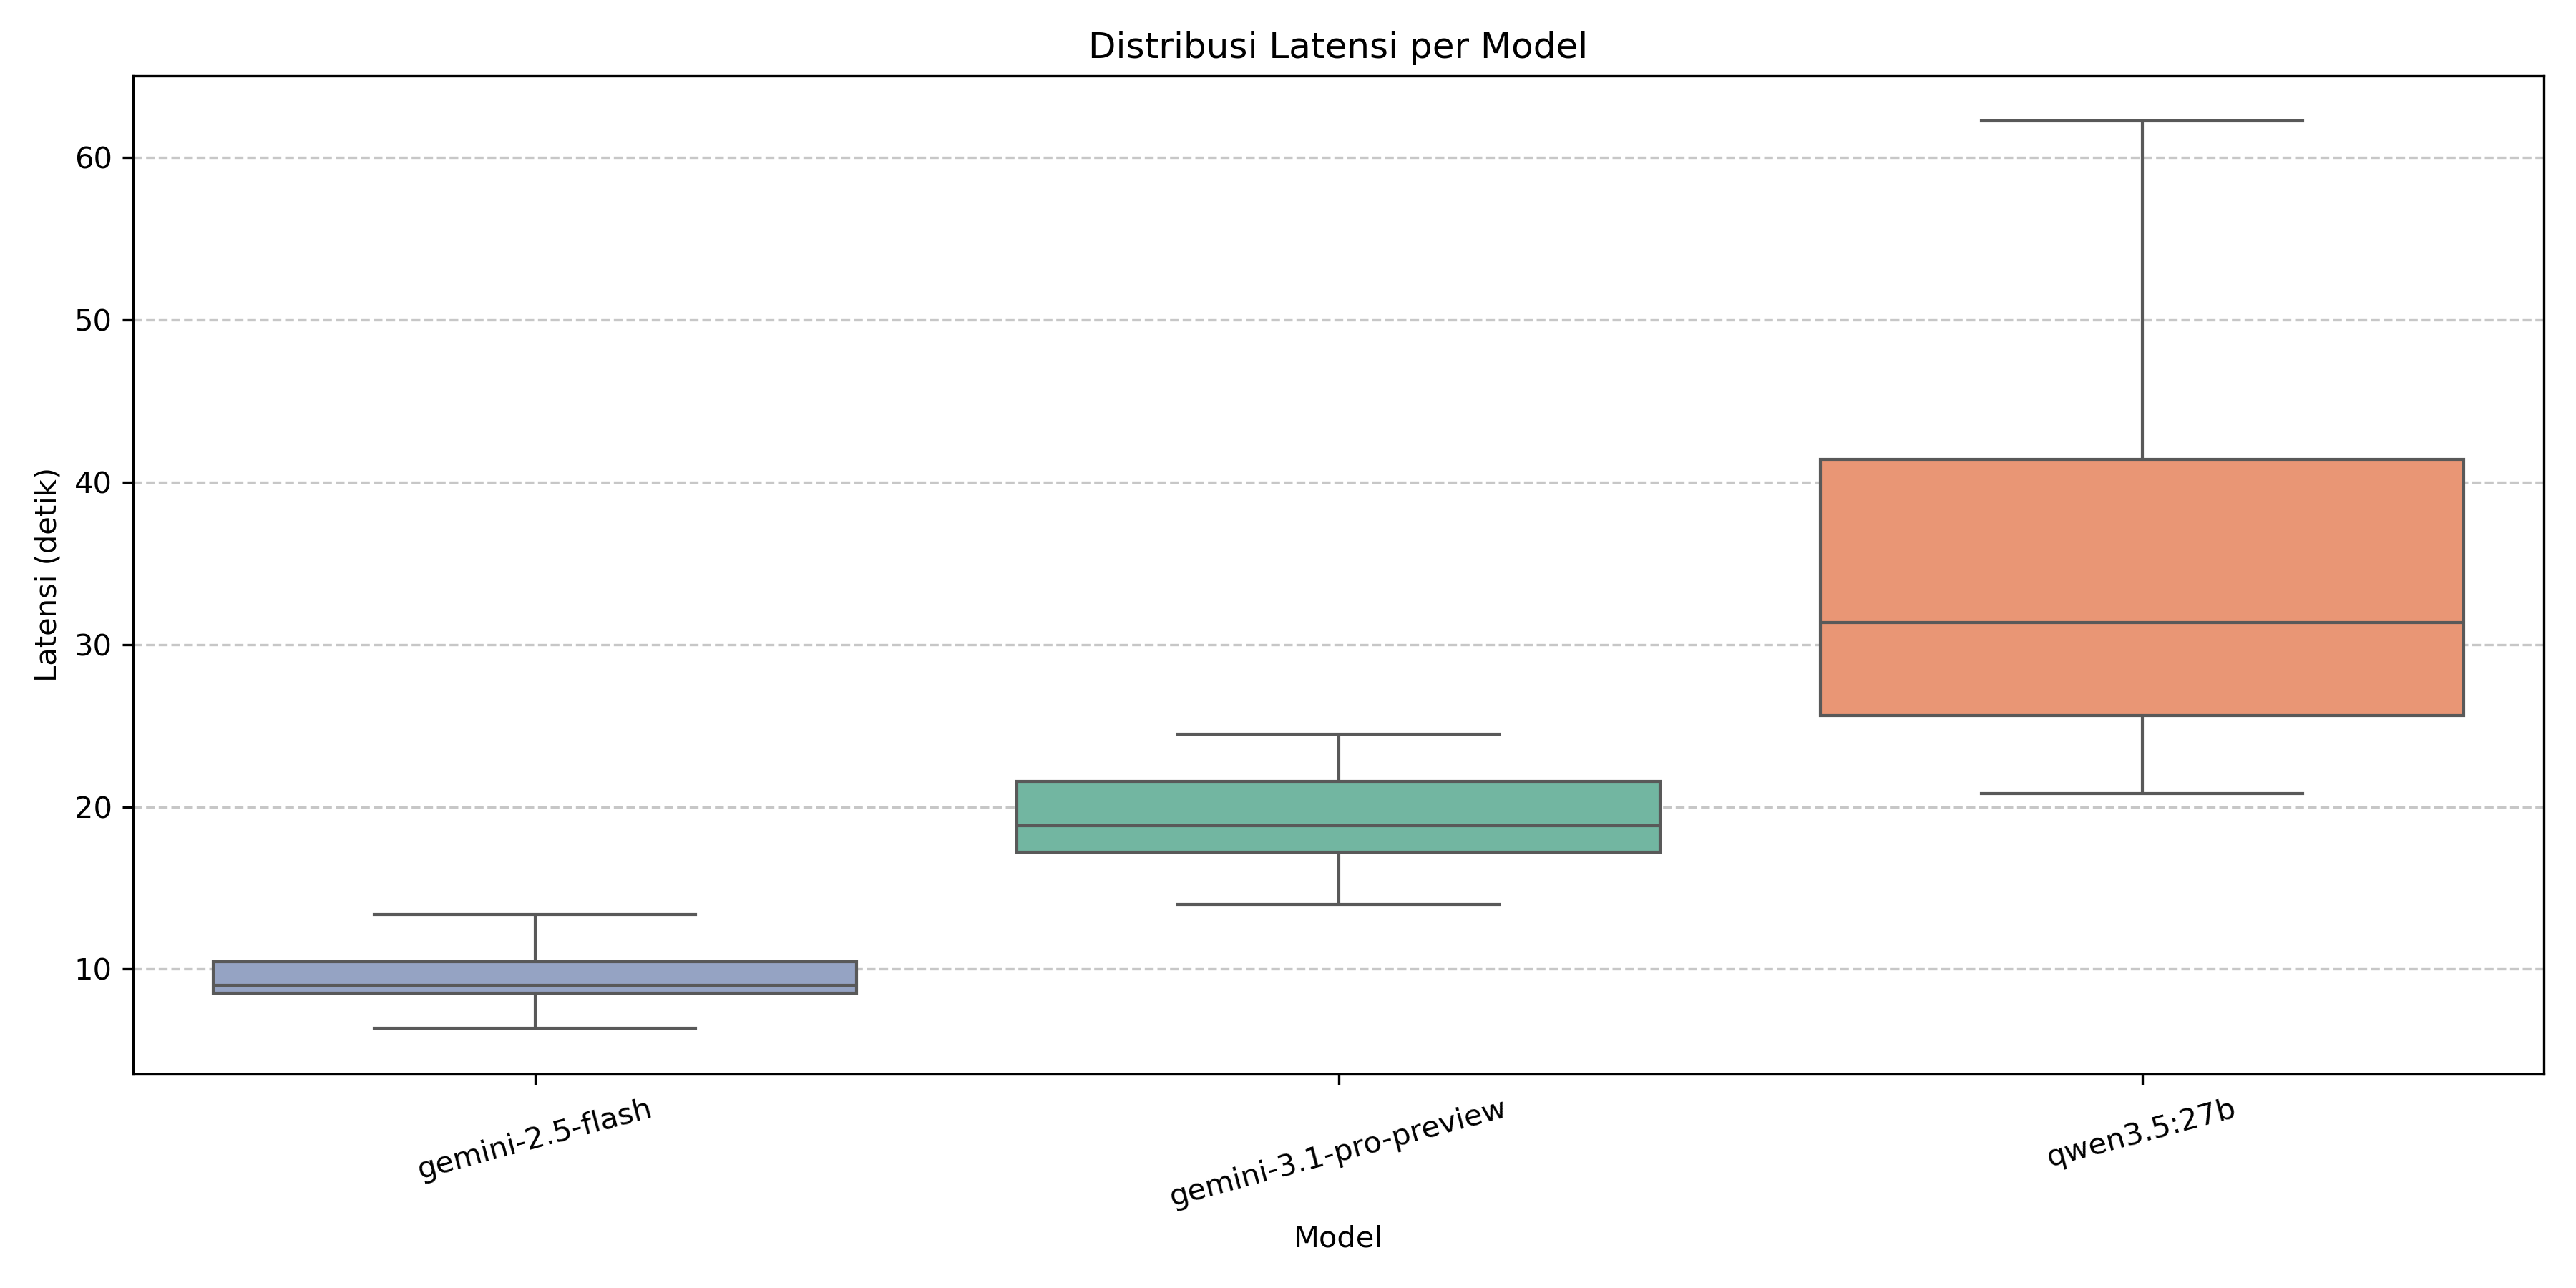
\includegraphics[width=0.8\textwidth]{Init/gambar/boxplots/boxplot_inspeksi_latensi.png}
    \caption{Distribusi Latensi Pengujian Analisis Objek per Model}
    \label{fig:boxplot_inspeksi_latensi}
\footnotesize \textbf{Sumber:} Dokumentasi Penulis
\end{figure}

\begin{figure}[H]
    \centering
    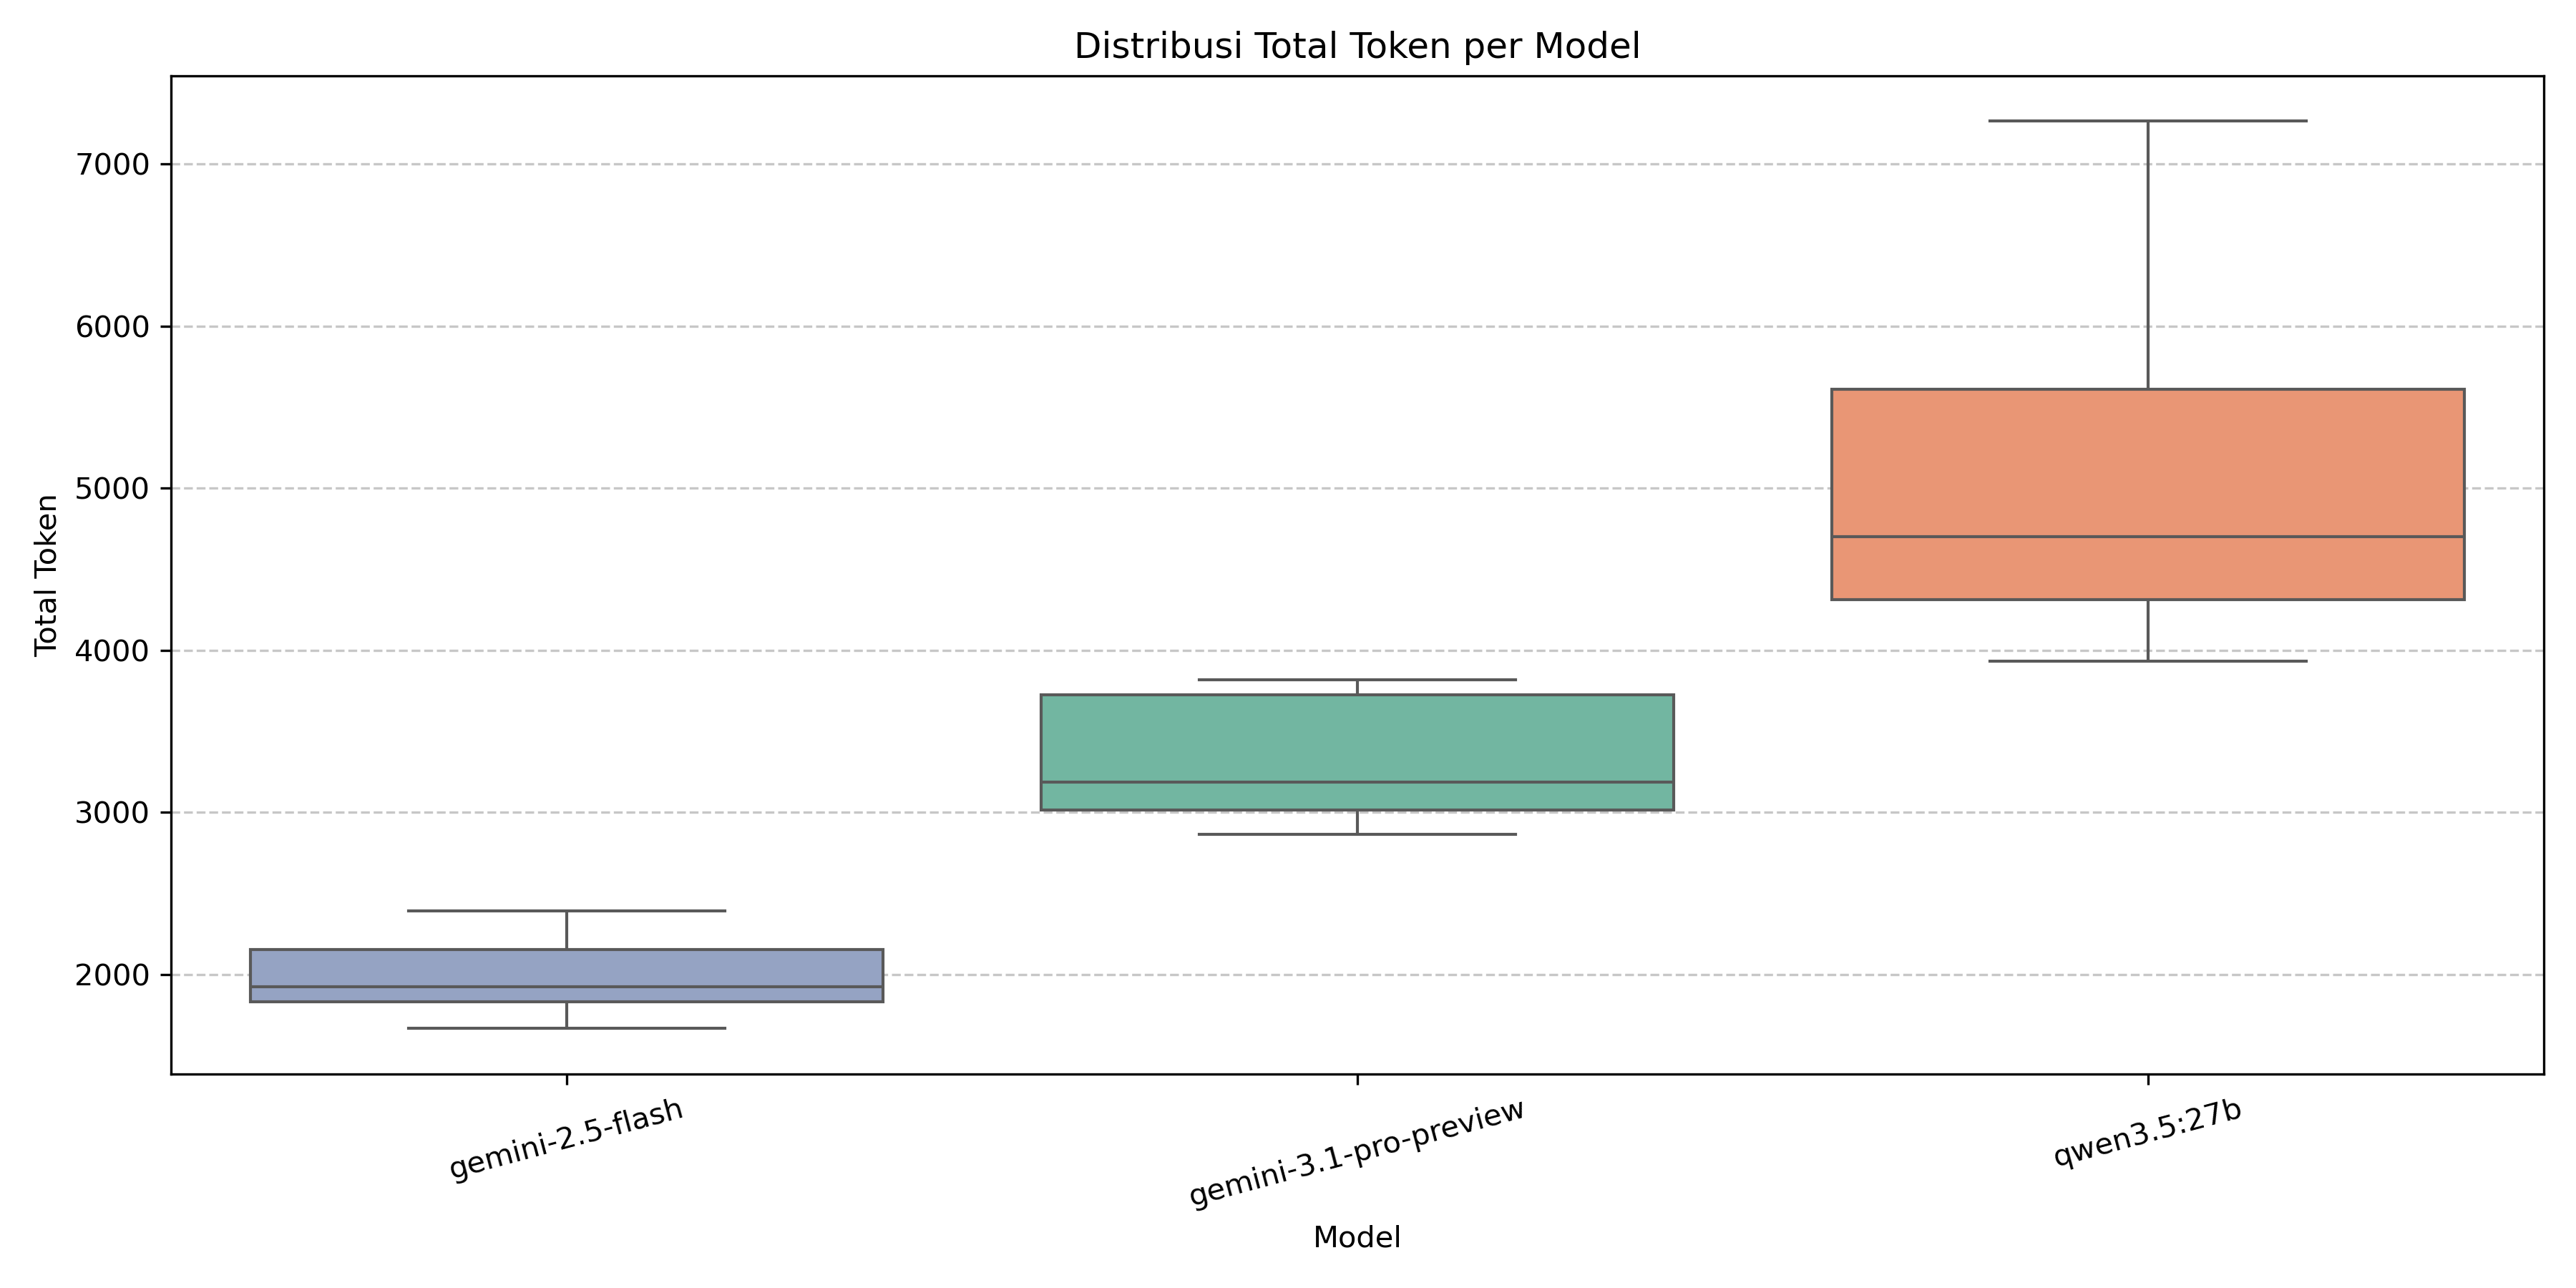
\includegraphics[width=0.8\textwidth]{Init/gambar/boxplots/boxplot_inspeksi_token.png}
    \caption{Distribusi Konsumsi Token Pengujian Analisis Objek per Model}
    \label{fig:boxplot_inspeksi_token}
\footnotesize \textbf{Sumber:} Dokumentasi Penulis
\end{figure}


\subsection{Analisis Data Keberhasilan}
Berdasarkan hasil pengujian pada Tabel \ref{tab:inspect_summary} dan Tabel \ref{tab:inspect_detail}, terlihat perbedaan performa yang signifikan antara model kelas atas dengan model yang lebih ringan dalam tugas analisis visual berbasis \textit{Multimodal Large Language Model} (MLLM). Gemini 3.1 Pro Preview mencatatkan performa sempurna dengan tingkat keberhasilan 100\% untuk seluruh kasus uji di berbagai variasi objek, kondisi, dan sudut pengambilan \textit{image}. Sebaliknya, Gemini 2.5 Flash dan Qwen 3.5 27B sama-sama mencatatkan tingkat keberhasilan 85,19\%. Meskipun tingkat kegagalan kedua model ini identik secara kuantitatif, analisis kualitatif terhadap respons model menunjukkan pola kegagalan yang berbeda.

Kasus ``selang APAR tidak menempel pada klip \textit{body}'' terbukti menjadi skenario paling menantang. Gemini 2.5 Flash mengalami kegagalan pada kondisi ini, di mana model berhalusinasi dengan menyatakan bahwa selang terpasang dengan baik. Qwen 3.5 juga mengalami kesulitan serupa karena memberikan hasil yang keliru terkait posisi ujung selang. Kegagalan pada skenario ini mengindikasikan kelemahan pada Flash dan Qwen dalam memahami detail spasial dan hubungan struktural antar komponen objek dari sebuah \textit{image}, tugas yang berhasil diselesaikan dengan baik oleh kapabilitas penalaran spasial Gemini 3.1 Pro.

Selain masalah penalaran spasial kompleks, Qwen 3.5 juga menunjukkan kelemahan pada tugas deteksi warna. Pada pengujian APAR dengan kondisi normal, Qwen 3.5 sempat gagal karena salah mengidentifikasi warna dominan tabung. Kesalahan deteksi ini berakar dari kondisi fisik APAR yang ditutupi oleh stiker label berwarna kuning pada sebagian besar tabungnya. Meskipun SOP secara eksplisit telah memberikan instruksi untuk mengabaikan warna label stiker, Qwen 3.5 terdistraksi oleh dominasi piksel kuning dan gagal mematuhi instruksi pengecualian tersebut. Kesalahan interpretasi warna semacam ini menjadi indikasi awal bahwa arsitektur \textit{Multimodal Large Language Model} pada dasarnya masih rentan terhadap jebakan visual mayoritas akibat dominasi warna tertentu, sebuah kerentanan komputasi visual yang bersifat stokastik dan berpotensi muncul pada model kelas atas sekalipun.

Kegagalan lain yang dialami oleh Flash dan Qwen terjadi pada skenario stop kontak dengan anomali steker putus atau rusak, di mana kedua model mengalami kesalahan \textit{false negative} dengan menyatakan kondisi steker aman dan utuh. Kegagalan ini menyoroti batasan resolusi dan kemampuan atensi model yang lebih kecil dalam mendeteksi anomali berskala detail ketika objek tersebut menempati proporsi piksel yang relatif kecil dibandingkan keseluruhan \textit{image}.

\subsection{Analisis Latensi dan Konsumsi \textit{Token}}
Berdasarkan distribusi latensi (Gambar \ref{fig:boxplot_inspeksi_latensi}) dan konsumsi token (Gambar \ref{fig:boxplot_inspeksi_token}), terlihat perubahan tren yang signifikan dibandingkan pengujian pemanggilan \textit{tool} sebelumnya akibat adanya penambahan dimensi multimodal berupa \textit{image}. Gemini 2.5 Flash tetap konsisten menjadi model tercepat dengan rata-rata latensi terendah. Sebaliknya, Qwen 3.5 mengalami pergeseran performa yang signifikan, jika pada pengujian berbasis teks sebelumnya model lokal ini cepat, pada analisis \textit{image} latensinya melonjak drastis menjadi yang terlama. Pembalikan tren ini terjadi karena proses ekstraksi fitur visual, kemungkinan memberi beban komputasi yang besar bagi perangkat keras lokal, melebihi beban pemrosesan instruksi teks murni. Gemini 3.1 Pro menunjukkan latensi yang lebih tinggi dibandingkan Gemini 2.5 Flash, sebanding dengan hasilnya yang mencapai akurasi sempurna pada seluruh skenario pengujian. Dari sisi penggunaan token, tren kesamaan antara kedua varian Gemini tidak lagi terlihat, kemungkinan akibat perbedaan mekanisme konversi \textit{image} ke \textit{image token}, Gemini 2.5 Flash mengonsumsi token paling sedikit berkat \textit{downscaling} resolusi, sedangkan Gemini 3.1 Pro menggunakan jauh lebih banyak demi mengekstrak fitur \textit{image} beresolusi tinggi. Sementara itu, Qwen 3.5 tetap konsisten menjadi model yang paling boros akibat inefisiensi arsitektur \textit{vision encoder} dan kecenderungannya memberikan penjelasan yang terlalu deskriptif.



% =============================================================================
% PENGUJIAN 3: PEMBUATAN PLAN
% =============================================================================
\section{Pengujian Pembuatan \textit{Plan} Inspeksi}
\label{sec:pengujian_plan}

\subsection{Tujuan Pengujian}
Pengujian ini bertujuan untuk mengevaluasi kemampuan model MLLM dalam menyusun rencana inspeksi yang optimal berdasarkan instruksi operator. Evaluasi mencakup kebenaran dalam mengidentifikasi objek target dari basis data, ketepatan urutan kunjungan berdasarkan efisiensi jarak terpendek dari posisi robot saat ini, serta kemampuan model dalam menolak permintaan yang tidak valid.

\subsection{Skenario Pengujian}
Dataset pengujian terdiri dari 12 kasus uji yang dibagi menjadi empat level kesulitan sebagai berikut:

\begin{enumerate}
    \item \textbf{Level Mudah} (1 objek target): Instruksi untuk menginspeksi satu objek tunggal. Model harus mengidentifikasi objek terdekat dan menyusun rencana sederhana. (3 kasus uji)
    \item \textbf{Level Sedang} (3 objek target): Instruksi untuk menginspeksi tiga objek dari kategori berbeda. Model harus mengurutkan kunjungan berdasarkan jarak terpendek. (3 kasus uji)
    \item \textbf{Level Sulit} (6 objek target): Instruksi untuk menginspeksi enam objek dari berbagai kategori. Model harus menyusun rute efisien untuk kunjungan yang lebih kompleks. (3 kasus uji)
    \item \textbf{Level Mustahil} (objek tidak valid): Instruksi yang meminta inspeksi objek atau lokasi yang tidak terdaftar dalam basis data. Model harus mampu menolak permintaan dan memberikan penjelasan. (3 kasus uji)
\end{enumerate}

Setiap kasus uji menyertakan posisi koordinat robot saat ini sebagai konteks tambahan untuk pengambilan keputusan urutan rute.

\subsection{Hasil Pengujian}

\begin{longtable}{|l|c|c|c|c|c|c|c|c|c|c|}
\caption{Hasil Pengujian Pembuatan \textit{Plan} Inspeksi} \label{tab:plan_results} \\
\hline
\multirow{2}{*}{\textbf{Level}} & \multirow{2}{*}{\textbf{\shortstack{Jumlah\\Objek}}} & \multicolumn{3}{c|}{\textbf{Gemini 2.5 Flash}} & \multicolumn{3}{c|}{\textbf{Gemini 3.1 Pro}} & \multicolumn{3}{c|}{\textbf{Qwen 3.5 27B}} \\
\cline{3-11}
& & \textbf{Skor} & \textbf{Rute} & \textbf{Latensi} & \textbf{Skor} & \textbf{Rute} & \textbf{Latensi} & \textbf{Skor} & \textbf{Rute} & \textbf{Latensi} \\
\hline
\endfirsthead
\hline
\multirow{2}{*}{\textbf{Level}} & \multirow{2}{*}{\textbf{\shortstack{Jumlah\\Objek}}} & \multicolumn{3}{c|}{\textbf{Gemini 2.5 Flash}} & \multicolumn{3}{c|}{\textbf{Gemini 3.1 Pro}} & \multicolumn{3}{c|}{\textbf{Qwen 3.5 27B}} \\
\cline{3-11}
& & \textbf{Skor} & \textbf{Rute} & \textbf{Latensi} & \textbf{Skor} & \textbf{Rute} & \textbf{Latensi} & \textbf{Skor} & \textbf{Rute} & \textbf{Latensi} \\
\hline
\endhead
Mudah & 1 & 2/3 & 2/2 & 17,88 & 3/3 & 3/3 & 19,44 & 2/3 & 2/2 & 22,06 \\
\hline
Sedang & 3 & 3/3 & 2/3 & 30,04 & 3/3 & 3/3 & 21,65 & 3/3 & 3/3 & 27,65 \\
\hline
Sulit & 6 & 3/3 & 3/3 & 43,45 & 3/3 & 3/3 & 26,64 & 3/3 & 1/3 & 28,33 \\
\hline
Mustahil & 0 & 3/3 & -- & 12,54 & 3/3 & -- & 19,65 & 3/3 & -- & 14,49 \\
\hline
\hline
\multicolumn{2}{|l|}{\textbf{\% Keberhasilan}} & \multicolumn{3}{c|}{91,67\%} & \multicolumn{3}{c|}{100,00\%} & \multicolumn{3}{c|}{91,67\%} \\
\hline
\multicolumn{2}{|l|}{\textbf{\% Rute Terpendek}} & \multicolumn{3}{c|}{87,50\%} & \multicolumn{3}{c|}{100,00\%} & \multicolumn{3}{c|}{75,00\%} \\
\hline
\multicolumn{2}{|l|}{\textbf{Rata-rata Latensi (s)}} & \multicolumn{3}{c|}{25,98} & \multicolumn{3}{c|}{21,85} & \multicolumn{3}{c|}{23,13} \\
\hline
\multicolumn{2}{|l|}{\textbf{Rata-rata Token}} & \multicolumn{3}{c|}{10.104} & \multicolumn{3}{c|}{5.565} & \multicolumn{3}{c|}{10.396} \\
\hline
\end{longtable}

\begin{figure}[H]
    \centering
    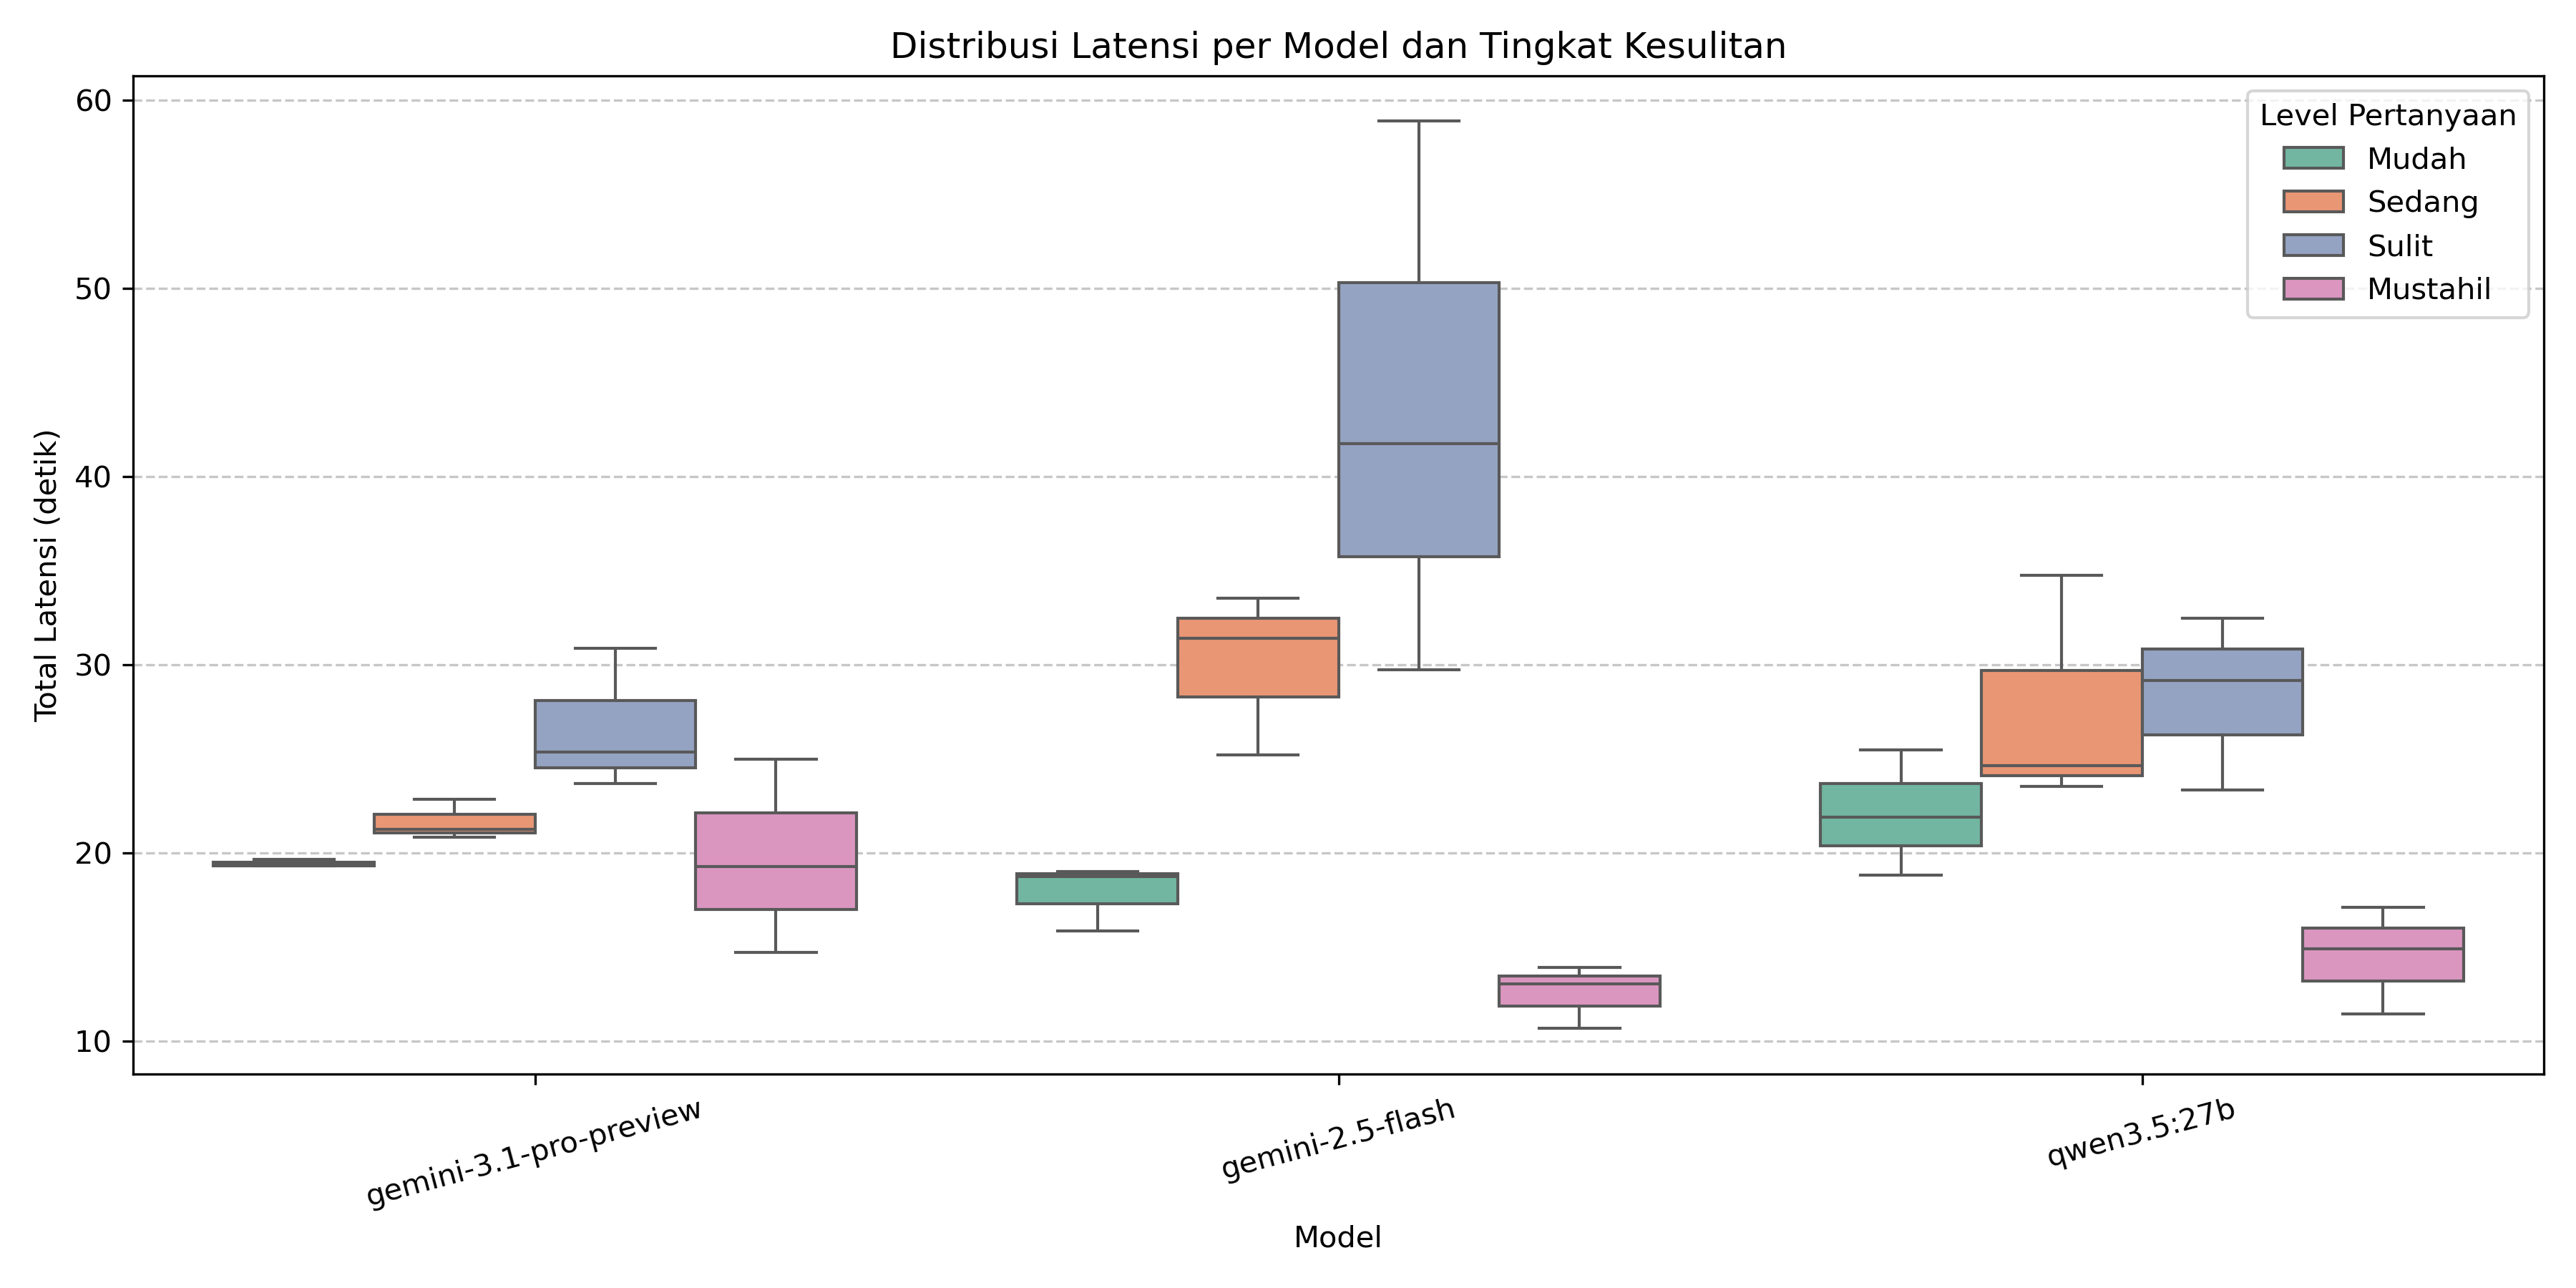
\includegraphics[width=0.8\textwidth]{Init/gambar/boxplots/boxplot_plan_latensi.png}
    \caption{Distribusi Latensi Pengujian Pembuatan \textit{Plan} per Model}
    \label{fig:boxplot_plan_latensi}
\footnotesize \textbf{Sumber:} Dokumentasi Penulis
\end{figure}

\begin{figure}[H]
    \centering
    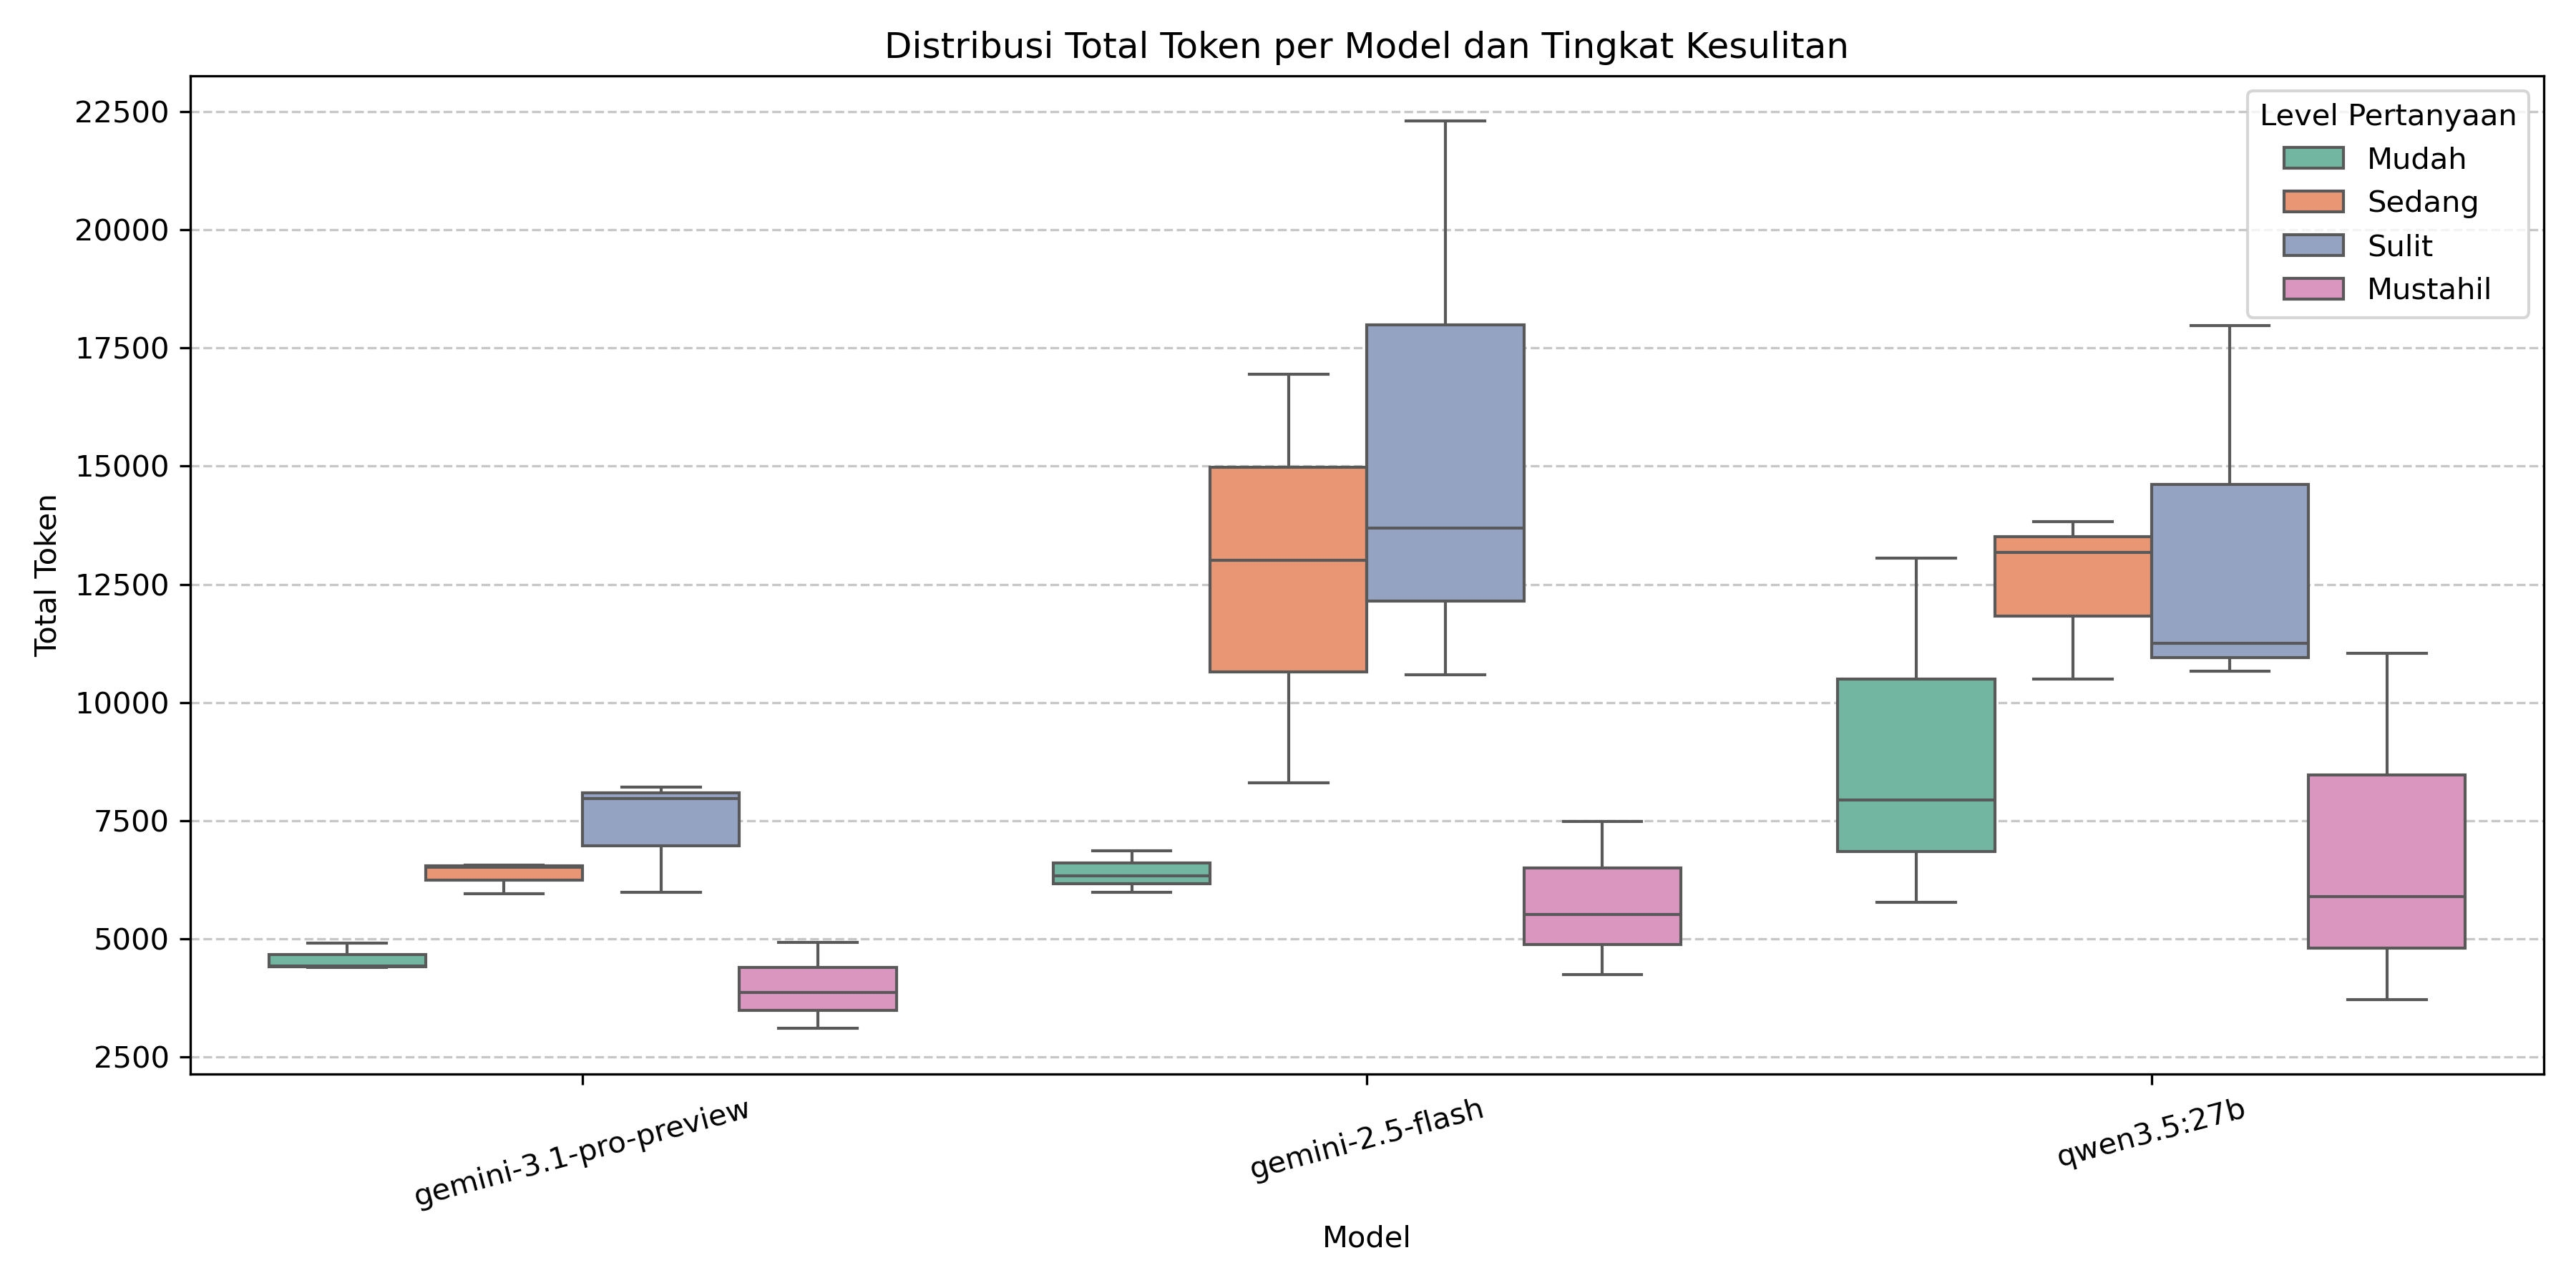
\includegraphics[width=0.8\textwidth]{Init/gambar/boxplots/boxplot_plan_token.png}
    \caption{Distribusi Konsumsi Token Pengujian Pembuatan \textit{Plan} per Model}
    \label{fig:boxplot_plan_token}
\footnotesize \textbf{Sumber:} Dokumentasi Penulis
\end{figure}


\subsection{Analisis Data Keberhasilan}
Berdasarkan hasil pengujian pada Tabel \ref{tab:plan_results}, kemampuan model dalam menyusun \textit{plan} inspeksi dievaluasi tidak hanya dari ketepatan pembuatan \textit{plan}, melainkan juga dari kemampuan penalaran matematis dan spasial untuk menyusun \textit{plan} yang efisien. Gemini 3.1 Pro Preview kembali menunjukkan dominasinya dengan tingkat keberhasilan skor dan rute terpendek mencapai 100\% di seluruh tingkat kesulitan. Sebaliknya, Gemini 2.5 Flash dan Qwen 3.5 mencatatkan tingkat keberhasilan pembuatan \textit{plan} sebesar 91,67\%, namun dengan tingkat efisiensi rute yang lebih rendah, yaitu 85,71\% untuk Flash dan 75,00\% untuk Qwen. Menariknya, ketiga model mencetak skor (100\%) pada level ``Mustahil'', menunjukkan kemampuan yang sangat baik dalam memvalidasi ketersediaan objek sebelum merencanakan rute, sehingga terhindar dari perencanaan halusinatif ketika objek yang diminta tidak ada di lingkungan.

Analisis terhadap kegagalan penyusunan rute pada Gemini 2.5 Flash dan Qwen 3.5 27B menunjukkan adanya satu kelemahan mendasar yang sama, yaitu kecenderungan menggunakan pendekatan \textit{greedy} yang berujung pada rute yang tidak optimal. Kedua model sering kali terjebak dengan hanya memilih objek terdekat dari posisi saat ini tanpa mempertimbangkan konsekuensi jarak akumulatif terhadap objek-objek selanjutnya. Pada Gemini 2.5 Flash, pendekatan ini menyebabkannya memilih objek terdekat yang justru menjauhkannya dari letak objek tujuan akhir, sehingga total jarak tempuh membengkak. Kesalahan identik juga dilakukan oleh Qwen 3.5, di mana model mengeksekusi inspeksi kumpulan objek searah secara berurutan, namun melewatkan satu objek di arah berlawanan, yang pada akhirnya memaksa robot melakukan manuver putar balik jarak jauh di akhir sesi. Kegagalan ini menegaskan bahwa kedua model tersebut memiliki keterbatasan arsitektur dalam memprediksi jarak secara menyeluruh.

Di sisi lain, Qwen 3.5 juga mengalami satu kegagalan berbeda terkait penalaran spasial, yang menyebabkan efisiensi rute menjadi lebih rendah dibandingkan model lainnya. Pada kasus tersebut, ketika dihadapkan pada beberapa kandidat objek, model tidak memilih objek terdekat untuk dimasukkan ke dalam rute, melainkan memilih objek yang posisinya lebih jauh dari kumpulan objek lainnya. Temuan ini menunjukkan bahwa pada kondisi tertentu Qwen 3.5 masih dapat mengalami kesalahan dalam membandingkan kedekatan spasial antar kandidat objek, yang berdampak pada kualitas rute inspeksi yang dihasilkan.

Selain permasalahan spasial tersebut, baik Gemini 2.5 Flash maupun Qwen 3.5 juga menunjukkan beberapa keterbatasan pada aspek lain. Gemini 2.5 Flash sempat gagal mematuhi batasan jumlah objek yang diinstruksikan, yaitu menyusun plan untuk tiga objek meskipun pengguna hanya meminta inspeksi terhadap satu objek. Sementara itu, Qwen 3.5 sempat mengalami kegagalan penyusunan plan akibat menghasilkan parameter yang tidak sesuai pada pemanggilan tool pencarian objek, sehingga tool tidak mengembalikan objek yang diharapkan.

\subsection{Analisis Latensi dan Konsumsi \textit{Token}}
Berdasarkan distribusi latensi (Gambar \ref{fig:boxplot_plan_latensi}) dan konsumsi token (Gambar \ref{fig:boxplot_plan_token}), terlihat pembalikan tren efisiensi dibandingkan kedua pengujian sebelumnya. Gemini 2.5 Flash, yang secara konsisten menjadi model tercepat dan paling efisien pada pengujian pemanggilan \textit{tool} murni maupun analisis \textit{image}, kini justru menunjukkan performa terburuk, latensi dan konsumsi tokennya melonjak, terutama pada level sedang dan sulit. Perubahan tren ini mengindikasikan bahwa Gemini 2.5 Flash membutuhkan proses penalaran yang lebih panjang ketika menangani perencanaan rute dengan banyak objek. Hal tersebut tercermin dari meningkatnya jumlah token yang dihasilkan, yang kemudian berdampak pada kenaikan latensi. Sebaliknya, Gemini 3.1 Pro justru menampilkan hasil yang paling efisien. Kemampuan penalaran pada Gemini Pro yang sebelumnya membuatnya tampak lebih lambat di pengujian dasar, kini terbukti lebih efisien untuk memecahkan masalah rute kompleks secara langsung tanpa memerlukan respon yang panjang. Sementara itu, Qwen 3.5 menunjukkan tren yang konsisten dengan pengujian sebelumnya, yakni mengonsumsi token dalam jumlah besar akibat format respons yang panjang, sehingga latensi inferensinya di server lokal pun tetap tinggi. Temuan ini menunjukkan bahwa efisiensi inferensi sangat dipengaruhi oleh kesesuaian antara karakteristik model dan kompleksitas tugas yang diberikan, model ringan yang dirancang untuk kecepatan, seperti Gemini Flash, akan mengalami pembengkakan token saat dipaksa menyelesaikan tugas penalaran tingkat tinggi, sementara model kompleks, seperti Gemini Pro, akan mengeksekusinya secara efisien.



% =============================================================================
% PENGUJIAN 4: KESELURUHAN SISTEM (END-TO-END)
% =============================================================================
\section{Pengujian Keseluruhan Sistem}
\label{sec:pengujian_e2e}

Pengujian ini bertujuan untuk mengevaluasi kinerja sistem secara menyeluruh dari awal hingga akhir (\textit{end-to-end}) dalam skenario inspeksi visual yang realistis. Pengujian mengukur kemampuan integrasi seluruh komponen sistem, mulai dari pembuatan rencana inspeksi, navigasi robot ke lokasi target, pengambilan dan analisis \textit{image}, hingga mekanisme intervensi operator (\textit{Human-in-the-Loop}).

\subsection{Skenario Pengujian}
Pengujian \textit{end-to-end} dirancang dalam tiga tingkat kesulitan (mudah, sedang, sulit) dengan tiga variasi skenario pada setiap tingkat. Lingkungan yang digunakan pada pengujian ini direpresentasikan oleh peta pada \textit{image} \ref{fig:map_annotated_e2e}. Pada peta tersebut, lokasi objek-objek inspeksi ditandai dengan lingkaran berwarna, di mana setiap jenis objek memiliki warna yang berbeda sesuai dengan keterangan pada legenda. Secara keseluruhan, terdapat 4 APAR, 3 stop kontak, dan 2 tong sampah yang tersebar di area pengujian. 

\begin{figure}[H]
    \centering
    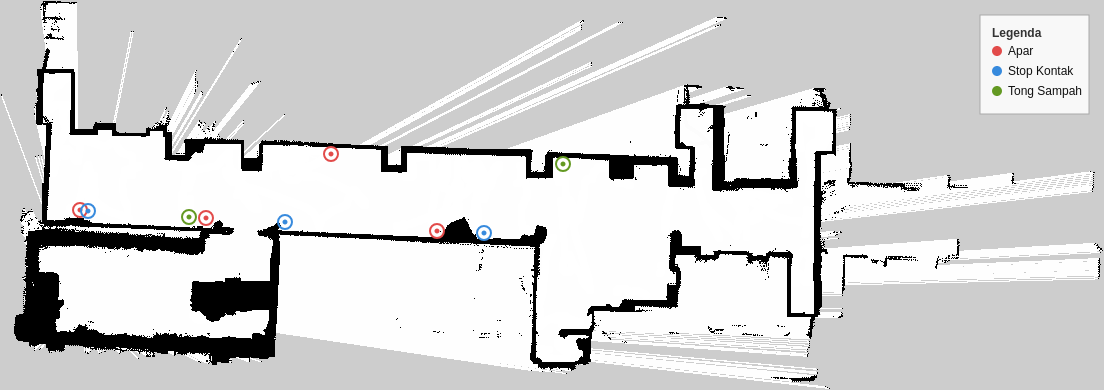
\includegraphics[width=0.8\textwidth]{Init/gambar/map_annotated.png}
    \caption{Peta Lingkungan Pengujian \textit{End-to-End} dengan Penanda Lokasi Objek}
    \label{fig:map_annotated_e2e}
\footnotesize \textbf{Sumber:} Dokumentasi Penulis
\end{figure}

Berikut adalah rincian seluruh skenario pengujian beserta instruksi awal yang diberikan kepada agen robot:

\renewcommand{\arraystretch}{1.5}
\begin{longtable}{|c|p{4cm}|p{8.5cm}|}
\caption{Detail Skenario Pengujian Keseluruhan Sistem (\textit{End-to-End})} \label{tab:skenario_e2e} \\
\hline
\textbf{Level} & \textbf{Skenario} & \textbf{Deskripsi dan Instruksi Pengguna} \\
\hline
\endfirsthead
\multicolumn{3}{c}%
{{Tabel \ref{tab:skenario_e2e} lanjutan dari halaman sebelumnya}} \\
\hline
\textbf{Level} & \textbf{Skenario} & \textbf{Deskripsi dan Instruksi Pengguna} \\
\hline
\endhead
\hline \multicolumn{3}{|r|}{{Lanjut ke halaman berikutnya}} \\ \hline
\endfoot
\hline
\endlastfoot

Mudah & Skenario 1 & Inspeksi 1 APAR berkondisi normal, Tanpa intervensi user. \newline \textbf{Instruksi:} \textit{``tolong inspeksi satu APAR terdekat di lantai 9''} \\
\cline{2-3}
& Skenario 2 & Inspeksi 1 APAR dengan anomali 'APAR di lantai', Tanpa intervensi user. \newline \textbf{Instruksi:} \textit{``tolong periksa kondisi satu APAR terdekat di lantai 9''} \\
\cline{2-3}
& Skenario 3 & Inspeksi 1 APAR dengan anomali 'selang tidak terpasang pada clip body', Dengan intervensi user mengubah plan sebelum dimulai (meminta robot duduk setelah inspeksi selesai). \newline \textbf{Instruksi:} \textit{``tolong inspeksi satu APAR terdekat di lantai 9''} \\
\hline

Sedang & Skenario 1 & Inspeksi 3 objek berbeda (1 APAR, 1 stop kontak, 1 tong sampah) yang semuanya normal, Tanpa intervensi user. \newline \textbf{Instruksi:} \textit{``tolong lakukan inspeksi pada satu APAR, satu stop kontak, dan satu tong sampah terdekat di lantai 9''} \\
\cline{2-3}
& Skenario 2 & Inspeksi 3 objek berbeda (1 APAR dengan anomali 'selang tidak terpasang pada clip body', 1 stop kontak dengan anomali 'terdapat steker', 1 tong sampah dengan anomali 'tong sampah berantakan banyak sampah'), Tanpa intervensi user. \newline \textbf{Instruksi:} \textit{``inspeksi satu APAR, satu stop kontak, dan satu tong sampah terdekat di lantai 9''} \\
\cline{2-3}
& Skenario 3 & Inspeksi objek berbeda (1 APAR dengan anomali 'selang tidak terpasang pada clip body', 1 stop kontak normal), Dengan intervensi user mengubah plan di tengah misi (saat robot di stop kontak, user minta penambahan inspeksi tong sampah). \newline \textbf{Instruksi:} \textit{``tolong periksa satu APAR, dan satu stop kontak terdekat di lantai 9''} \\
\hline

Sulit & Skenario 1 & Inspeksi 6 objek (2 APAR, 2 stop kontak, 2 tong sampah), Kondisi: 3 objek normal, 3 objek anomali (1 APAR di lantai, 1 steker rusak, 1 tong sampah tidak lengkap), Tanpa intervensi user. \newline \textbf{Instruksi:} \textit{``tolong lakukan inspeksi ke dua APAR, dua stop kontak, dan dua tong sampah terdekat di lantai 9''} \\
\cline{2-3}
& Skenario 2 & Inspeksi 6 objek (1 APAR normal, 1 APAR di lantai, 1 APAR dengan selang tidak terpasang pada clip body, 1 stop kontak dengan steker rusak, 1 tong sampah tidak lengkap, 1 tong sampah normal), Dengan intervensi user membatalkan 1 stop kontak dan menambah 1 tong sampah. \newline \textbf{Instruksi:} \textit{``tolong inspeksi tiga APAR, dua stop kontak, dan satu tong sampah terdekat di lantai 9''} \\
\cline{2-3}
& Skenario 3 & Inspeksi 6 objek (1 APAR normal, 1 APAR di lantai, 2 APAR dengan selang tidak terpasang pada clip body, 1 stop kontak normal, 1 tong sampah dengan sampah berserakan), Dengan intervensi user, saat robot sampai di salah satu APAR yang memiliki anomali, user menginstruksikan robot untuk maju mendekat. \newline \textbf{Instruksi:} \textit{``tolong periksa empat APAR, satu stop kontak, dan satu tong sampah terdekat di lantai 9''} \\
\end{longtable}

Parameter evaluasi meliputi keberhasilan pembuatan \textit{plan}, keberhasilan \textit{plan} jarak terpendek, keberhasilan analisis objek, keberhasilan penanganan intervensi, total waktu sesi, total token sesi, dan jumlah pemanggilan \textit{tool}.

\subsection{Hasil Pengujian}

% --- Tabel Ringkasan E2E ---
\begin{table}[H]
\centering
\caption{Ringkasan Hasil Pengujian \textit{End-to-End}}
\label{tab:e2e_summary}
\renewcommand{\arraystretch}{1.2}
\resizebox{\linewidth}{!}{
\begin{tabular}{|l|c|c|c|}
\hline
\textbf{Metrik} & \textbf{Gemini 2.5 Flash} & \textbf{Gemini 3.1 Pro} & \textbf{Qwen 3.5 27B} \\
\hline
Keberhasilan \textit{Plan} & 100,00\% & 100,00\% & 100,00\% \\
\hline
\textit{Plan} Rute Terpendek & 77,78\% & 100,00\% & 66,67\% \\
\hline
Keberhasilan Analisis Objek & 86,67\% & 93,33\% & 63,33\% \\
\hline
Keberhasilan Intervensi & 100,00\% & 100,00\% & 100,00\% \\
\hline
Rata-rata Waktu Sesi (detik) & 382,91 & 367,40 & 610,79 \\
\hline
Rata-rata Konsumsi Token & 153.564 & 183.440 & 140.072 \\
\hline
\end{tabular}
}
\end{table}

% --- Tabel Hasil E2E Gemini 2.5 Flash ---
\begin{longtable}{|c|c|c|c|c|c|c|c|}
\caption{Hasil Pengujian \textit{End-to-End} Model Gemini 2.5 Flash} \label{tab:e2e_flash} \\
\hline
\textbf{Level} & \textbf{Skenario} & \textbf{Plan} & \textbf{Rute} & \textbf{Analisis} & \textbf{Intervensi} & \textbf{Waktu (s)} & \textbf{Token} \\
\hline
\endfirsthead
\hline
\textbf{Level} & \textbf{Skenario} & \textbf{Plan} & \textbf{Rute} & \textbf{Analisis} & \textbf{Intervensi} & \textbf{Waktu (s)} & \textbf{Token} \\
\hline
\endhead
Mudah & 1 & \checkmark & \checkmark & 1/1 & -- & 84,89 & 34.922 \\
\hline
Mudah & 2 & \checkmark & \checkmark & 1/1 & -- & 64,54 & 32.876 \\
\hline
Mudah & 3 & \checkmark & \checkmark & 1/1 & \checkmark & 150,29 & 52.467 \\
\hline
Sedang & 1 & \checkmark & \checkmark & 3/3 & -- & 295,61 & 125.978 \\
\hline
Sedang & 2 & \checkmark & \checkmark & 2/3 & -- & 285,75 & 111.419 \\
\hline
Sedang & 3 & \checkmark & \checkmark & 3/3 & \checkmark & 335,43 & 126.673 \\
\hline
Sulit & 1 & \checkmark & \checkmark & 6/6 & -- & 591,96 & 248.842 \\
\hline
Sulit & 2 & \checkmark & $\times$ & 5/6 & \checkmark & 775,59 & 279.289 \\
\hline
Sulit & 3 & \checkmark & $\times$ & 4/6 & \checkmark & 862,10 & 369.609 \\
\hline
\end{longtable}

% --- Tabel Hasil E2E Gemini 3.1 Pro ---
\begin{longtable}{|c|c|c|c|c|c|c|c|}
\caption{Hasil Pengujian \textit{End-to-End} Model Gemini 3.1 Pro Preview} \label{tab:e2e_pro} \\
\hline
\textbf{Level} & \textbf{Skenario} & \textbf{Plan} & \textbf{Rute} & \textbf{Analisis} & \textbf{Intervensi} & \textbf{Waktu (s)} & \textbf{Token} \\
\hline
\endfirsthead
\hline
\textbf{Level} & \textbf{Skenario} & \textbf{Plan} & \textbf{Rute} & \textbf{Analisis} & \textbf{Intervensi} & \textbf{Waktu (s)} & \textbf{Token} \\
\hline
\endhead
Mudah & 1 & \checkmark & \checkmark & 1/1 & -- & 110,43 & 30.631 \\
\hline
Mudah & 2 & \checkmark & \checkmark & 1/1 & -- & 93,48 & 30.898 \\
\hline
Mudah & 3 & \checkmark & \checkmark & 1/1 & \checkmark & 145,12 & 45.712 \\
\hline
Sedang & 1 & \checkmark & \checkmark & 3/3 & -- & 294,14 & 173.103 \\
\hline
Sedang & 2 & \checkmark & \checkmark & 3/3 & -- & 277,23 & 115.623 \\
\hline
Sedang & 3 & \checkmark & \checkmark & 3/3 & \checkmark & 250,91 & 128.318 \\
\hline
Sulit & 1 & \checkmark & \checkmark & 6/6 & -- & 681,65 & 318.511 \\
\hline
Sulit & 2 & \checkmark & \checkmark & 5/6 & \checkmark & 560,26 & 332.709 \\
\hline
Sulit & 3 & \checkmark & \checkmark & 5/6 & \checkmark & 893,42 & 475.459 \\
\hline
\end{longtable}

% --- Tabel Hasil E2E Qwen 3.5 ---
\begin{longtable}{|c|c|c|c|c|c|c|c|}
\caption{Hasil Pengujian \textit{End-to-End} Model Qwen 3.5 27B} \label{tab:e2e_qwen} \\
\hline
\textbf{Level} & \textbf{Skenario} & \textbf{Plan} & \textbf{Rute} & \textbf{Analisis} & \textbf{Intervensi} & \textbf{Waktu (s)} & \textbf{Token} \\
\hline
\endfirsthead
\hline
\textbf{Level} & \textbf{Skenario} & \textbf{Plan} & \textbf{Rute} & \textbf{Analisis} & \textbf{Intervensi} & \textbf{Waktu (s)} & \textbf{Token} \\
\hline
\endhead
Mudah & 1 & \checkmark & \checkmark & 1/1 & -- & 105,29 & 25.678 \\
\hline
Mudah & 2 & \checkmark & \checkmark & 0/1 & -- & 100,85 & 31.529 \\
\hline
Mudah & 3 & \checkmark & \checkmark & 0/1 & \checkmark & 186,36 & 60.081 \\
\hline
Sedang & 1 & \checkmark & \checkmark & 3/3 & -- & 374,77 & 99.721 \\
\hline
Sedang & 2 & \checkmark & \checkmark & 2/3 & -- & 274,29 & 102.818 \\
\hline
Sedang & 3 & \checkmark & \checkmark & 3/3 & \checkmark & 397,54 & 108.792 \\
\hline
Sulit & 1 & \checkmark & $\times$ & 4/6 & -- & 1.550,64 & 231.210 \\
\hline
Sulit & 2 & \checkmark & $\times$ & 3/6 & \checkmark & 1.010,24 & 224.071 \\
\hline
Sulit & 3 & \checkmark & $\times$ & 3/6 & \checkmark & 1.497,17 & 376.747 \\
\hline
\end{longtable}
\begin{figure}[H]
    \centering
    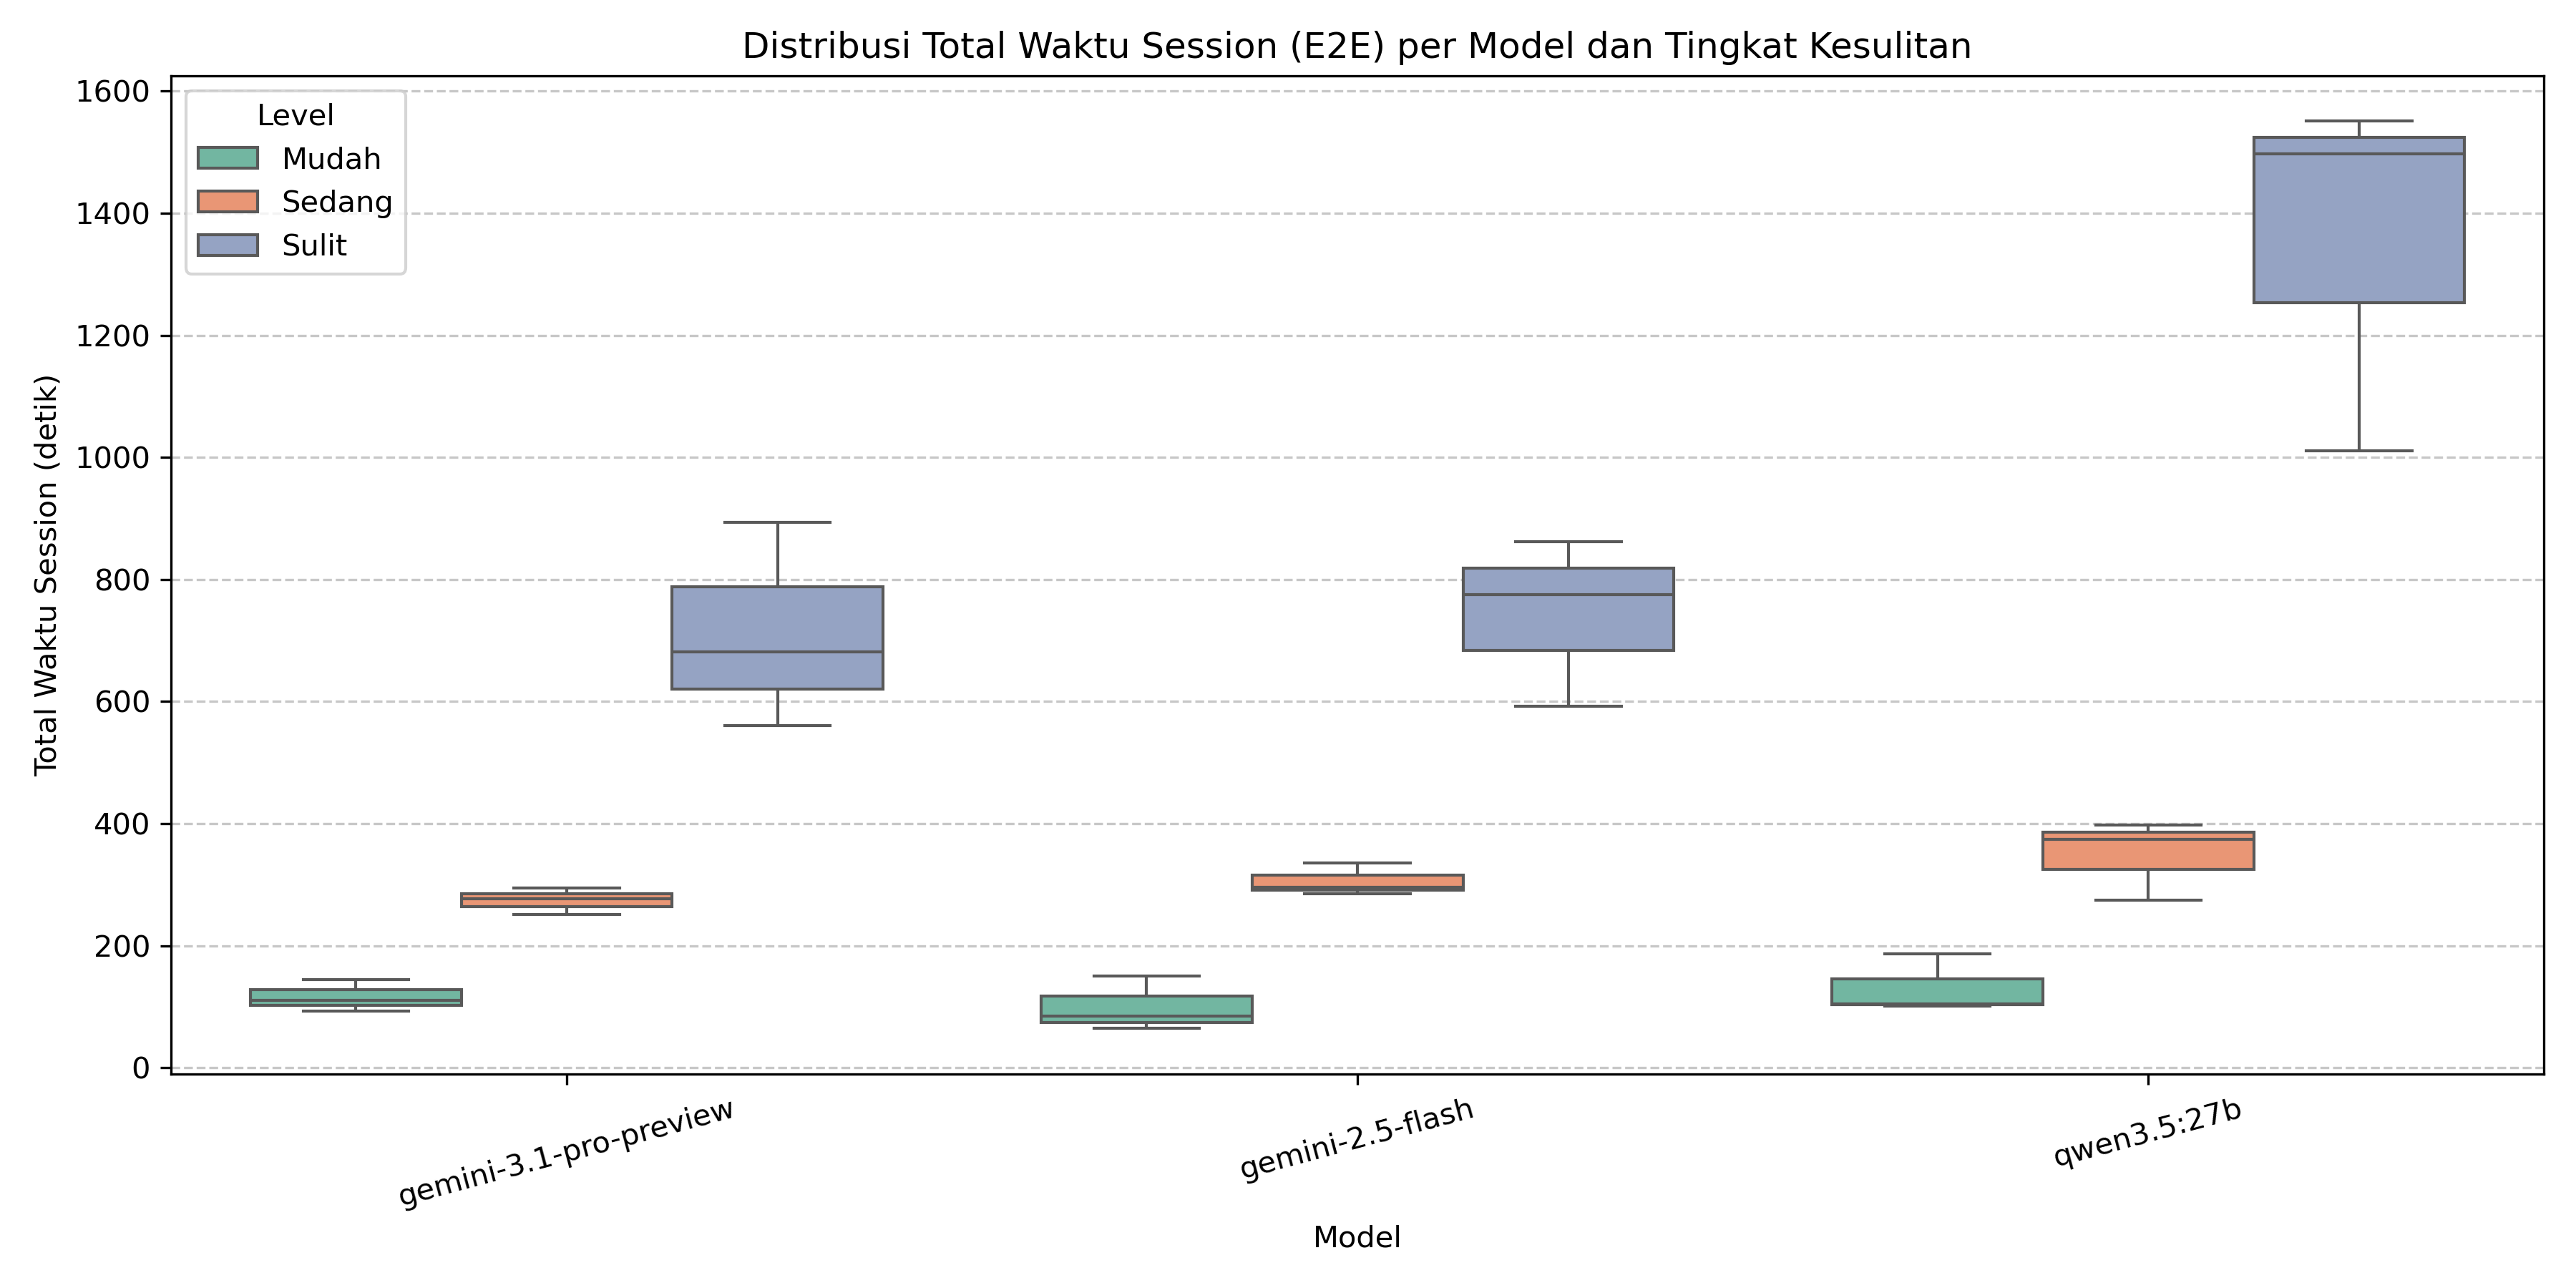
\includegraphics[width=0.8\textwidth]{Init/gambar/boxplots/boxplot_e2e_latensi.png}
    \caption{Distribusi Waktu Sesi Pengujian \textit{End-to-End} per Model}
    \label{fig:boxplot_e2e_latensi}
\footnotesize \textbf{Sumber:} Dokumentasi Penulis
\end{figure}

\begin{figure}[H]
    \centering
    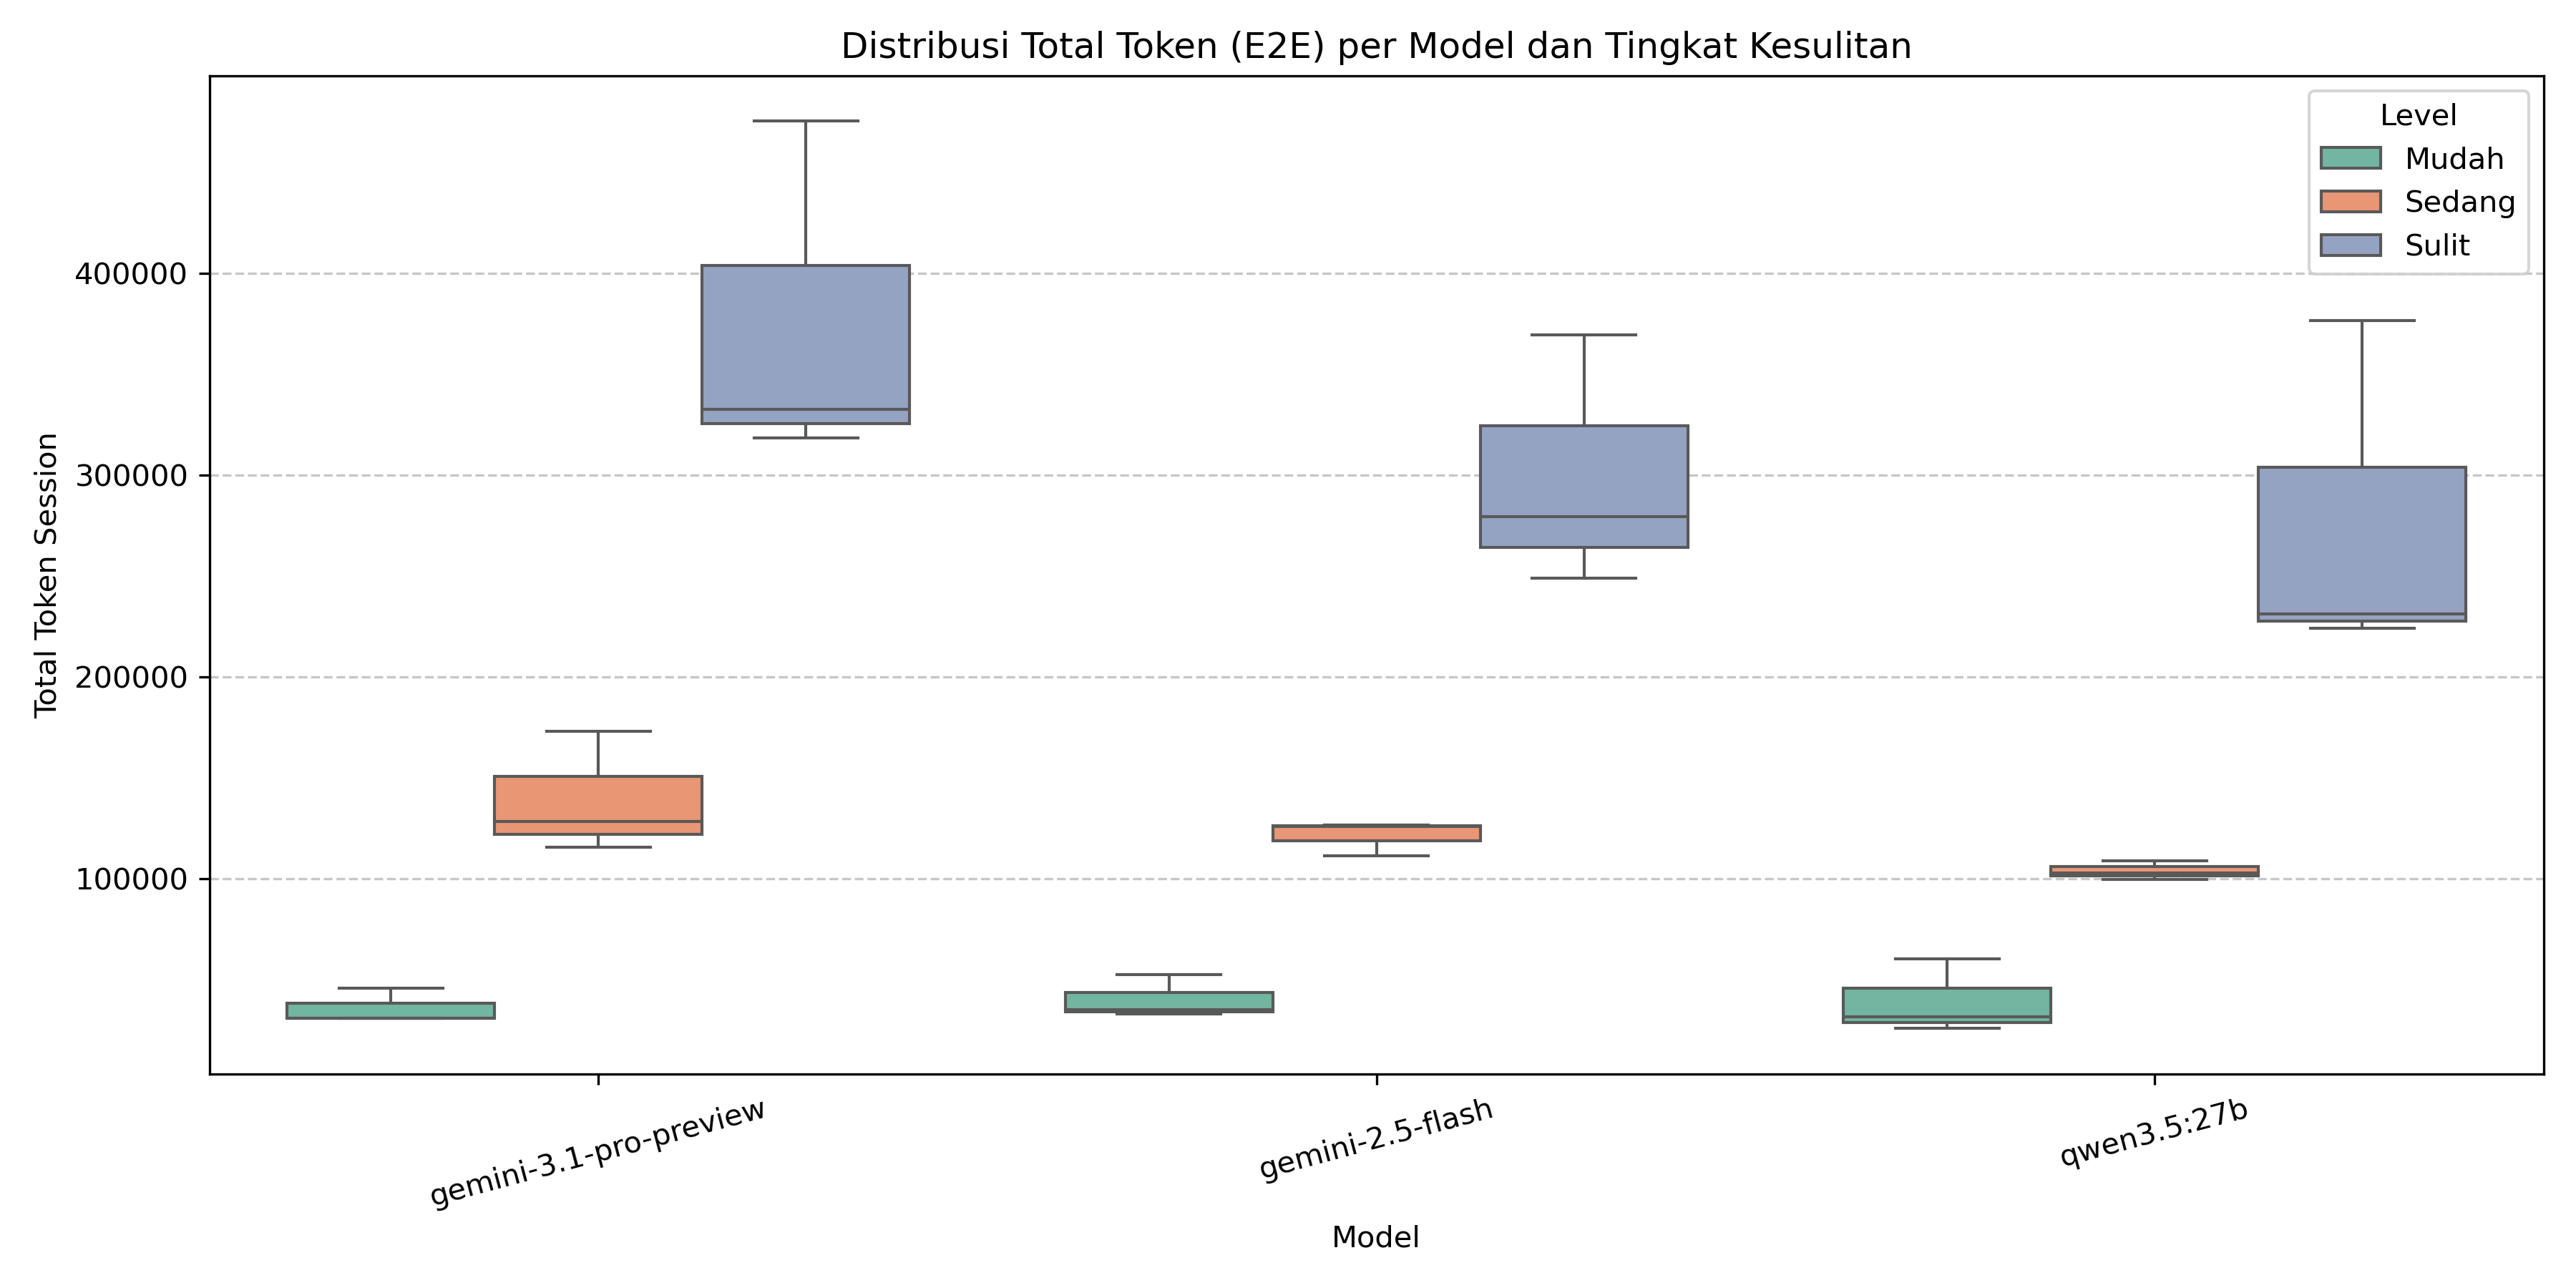
\includegraphics[width=0.8\textwidth]{Init/gambar/boxplots/boxplot_e2e_token.png}
    \caption{Distribusi Konsumsi Token Pengujian \textit{End-to-End} per Model}
    \label{fig:boxplot_e2e_token}
\footnotesize \textbf{Sumber:} Dokumentasi Penulis
\end{figure}

\subsection{Analisis Data Keberhasilan}
Berdasarkan hasil pengujian pada Tabel \ref{tab:e2e_summary}, \ref{tab:e2e_flash}, \ref{tab:e2e_pro}, dan \ref{tab:e2e_qwen}, sistem inspeksi otonom menunjukkan tingkat keberhasilan dasar yang tinggi. Ketiga model berhasil mencatatkan persentase 100\% pada keberhasilan pembuatan \textit{plan} awal di seluruh variasi skenario, termasuk saat terjadi intervensi operator. Hal ini membuktikan bahwa integrasi agen MLLM berjalan stabil dalam mengonversi keputusan teks menjadi aksi pergerakan fisik robot. Seluruh model juga terbukti adaptif dalam merespons instruksi intervensi operator, baik berupa perubahan rencana, instruksi manuver tambahan, maupun penambahan objek baru di tengah misi. Sedangkan, dalam aspek perencanaan rute, Gemini 3.1 Pro terbukti sangat andal dengan mempertahankan rekor 100\% rute terpendek. Di sisi lain, keterbatasan arsitektur penalaran spasial pada Gemini 2.5 Flash dan Qwen 3.5 kembali terlihat jelas. Flash gagal menentukan rute paling efisien pada skenario Sulit Skenario 2 dan Skenario 3 akibat pola pendekatan \textit{greedy} yang tidak optimal, sementara Qwen 3.5 secara konsisten gagal menyusun rute terpendek di seluruh skenario level Sulit.

Perbedaan performa antar model terlihat signifikan pada evaluasi akurasi analisis visual di lapangan. Gemini 3.1 Pro Preview kembali menjadi yang terbaik dengan keberhasilan analisis objek mencapai 93,33\% dari keseluruhan objek uji di berbagai skenario. Dua kegagalan analisis pada model ini hanya terjadi pada skenario Sulit Skenario 2 (salah mengidentifikasi APAR merah menjadi kuning) dan Sulit Skenario 3 (salah mengidentifikasi selang APAR normal menjadi terlepas). Di urutan kedua, Gemini 2.5 Flash mencatatkan keberhasilan sebesar 86,67\%. Analisis menunjukkan pola kegagalan yang konsisten, khususnya pada deteksi warna APAR. Pada skenario Sedang Skenario 2 Gemini 2.5 Flash dan Sulit Skenario 2 Gemini 3.1 Pro, MLLM menyimpulkan bahwa tabung APAR berwarna kuning. Menariknya, kesalahan deteksi akibat dominasi piksel kuning dari stiker label ini sebelumnya hanya dialami oleh model Qwen 3.5 pada pengujian analisis \textit{image}. Fakta bahwa kedua varian Gemini akhirnya ikut terdistraksi oleh jebakan visual yang sama menegaskan bahwa kerentanan terhadap dominasi warna mayoritas merupakan kelemahan bawaan  pada MLLM. Meskipun SOP telah dirancang secara eksplisit untuk mengabaikan warna label, MLLM secara general ada kalanya tetap terkecoh dan mengabaikan instruksi pengecualian tersebut. Selain masalah warna, Flash juga keliru menyatakan selang APAR menempel rapi pada klipnya pada skenario Sulit Skenario 3.

Sementara itu, Qwen 3.5 27B mengalami degradasi performa analisis visual yang sangat drastis dalam skenario \textit{end-to-end}, dengan tingkat keberhasilan hanya mencapai 63,33\%. Qwen berulang kali menghasilkan \textit{false positive}. Pada tingkat Mudah, model ini gagal mendeteksi anomali APAR yang jatuh di lantai dan menganggapnya tergantung normal di dinding, serta menganggap selang yang terlepas sebagai kondisi normal. Kegagalan ini terus berulang di level Sedang dan Sulit. Selain kelemahan pemahaman spasial, Qwen 3.5 juga mengalami kesalahan persepsi warna, menyatakan warna APAR pudar padahal aman. Secara umum, tingginya penurunan persentase keberhasilan analisis objek pada pengujian \textit{end-to-end} secara kuantitatif, terutama pada Qwen 3.5 dan Gemini 2.5 Flash, sebenarnya sangat dipengaruhi oleh komposisi \textit{dataset} skenario. Pengujian \textit{end-to-end} melibatkan repetisi yang jauh lebih tinggi untuk skenario anomali "selang APAR tidak menempel pada klip \textit{body}". Pada pengujian analisis \textit{image} sebelumnya, anomali struktural ini telah terbukti sebagai kasus spasial yang paling menantang dan paling sering mengecoh pemahaman spasial MLLM. Dengan tingginya frekuensi kemunculan skenario tersebut di sepanjang pengujian \textit{end-to-end}, performa kuantitatif model secara matematis akan mengalami penurunan yang signifikan.

\subsection{Analisis Waktu Sesi dan Konsumsi \textit{Token}}
Berdasarkan distribusi waktu sesi (Gambar \ref{fig:boxplot_e2e_latensi}) dan konsumsi token (Gambar \ref{fig:boxplot_e2e_token}), ditemukan sebuah anomali performa latensi yang membedakan pengujian keseluruhan sistem dengan pengujian terisolasi. Dari sisi waktu penyelesaian misi, Gemini 2.5 Flash awalnya berhasil menunjukkan latensi tercepat tingkat Mudah. Namun, pada level Sedang dan Sulit, latensi Flash meningkat drastis hingga menyamai bahkan melampaui lambatnya waktu eksekusi Gemini 3.1 Pro. Temuan ini sangat kontraintuitif dengan hasil pengujian analisis \textit{image} terisolasi sebelumnya, di mana Flash terbukti jauh lebih cepat memproses input visual dibandingkan Pro. Mengingat pada skenario \textit{end-to-end} proses pembuatan \textit{plan} hanya dieksekusi satu kali di awal misi, sedangkan pemanggilan \textit{tool} analisis \textit{image} dieksekusi berulang kali di setiap titik, secara matematis Flash seharusnya mendominasi kecepatan misi secara keseluruhan. Berkurangnya keunggulan waktu Flash secara signifikan ini kemungkinan disebabkan oleh adanya latensi jaringan yang tidak sama antara Gemini Flash dan Pro saat pengujian berlangsung. Hal inilah yang menyebabkan waktu eksekusi keseluruhan Flash seolah-olah tersusul dan melambat jika dibandingkan dengan Pro.

Di sisi lain, Qwen 3.5 mencatatkan waktu sesi yang sangat tinggi pada level Sulit, berkisar antara 17 hingga 26 menit. Lamanya waktu eksekusi ini merupakan akumulasi dari dua faktor utama, yaitu kelemahan inferensi Qwen pada pengujian analisis \textit{image}, di mana latensi ekstraksi fitur visual beruntun untuk banyak objek memberikan beban komputasi. Dari sisi konsumsi token, terlihat perbedaan tren yang menarik. Jika pada pengujian terisolasi Qwen 3.5 atau Gemini Flash sering menjadi yang paling boros token, pada skenario \textit{end-to-end} Gemini 3.1 Pro justru mencatatkan konsumsi token yang lebih tinggi. Penelusuran pada kode \textit{backend} mengonfirmasi bahwa perbedaan ini tidak semata-mata disebabkan oleh performa model, melainkan oleh berbedanya mekanisme serialisasi \textit{tool response} pada protokol API. Meskipun \textit{payload} balasan yang dikirimkan ke model adalah identik, Gemini API membungkus hasil \textit{tool} secara terstruktur menggunakan Part.from\_function\_response, sementara \textit{endpoint} Qwen 3.5 cukup menyerialisasinya menjadi string JSON standar melalui json.dumps(). Perbedaan format ini membuat Gemini secara tak terduga menghabiskan jauh lebih banyak token saat memproses hasil \textit{tool} dengan struktur data bersarang, sehingga selisih konsumsi token akhir pada pengujian \textit{end-to-end} ini sebagian besar merupakan konsekuensi dari penumpukan konteks respon \textit{tool}.



% =============================================================================
% PENGUJIAN 5: NASA-TLX
% =============================================================================
\section{Pengujian Beban Kerja Operator (NASA-TLX)}
\label{sec:pengujian_nasa_tlx}

Pengujian ini bertujuan untuk mengukur beban kerja yang dirasakan oleh operator saat menjalankan misi inspeksi menggunakan metode NASA Task Load Index (NASA-TLX). Hasil pengujian ini digunakan untuk mengevaluasi sejauh mana sistem yang dikembangkan dapat mengurangi beban kerja operator dibandingkan dengan metode inspeksi konvensional.

\subsection{Skenario Pengujian}
Pengujian dilakukan dengan melibatkan 10 responden yang masing-masing diminta untuk mengevaluasi beban kerja pada tiga kondisi inspeksi yang berbeda:

\begin{enumerate}
    \item \textbf{Inspeksi Keseluruhan Manual}: Operator mengendalikan robot secara penuh menggunakan teleoperasi manual untuk navigasi, pengambilan \textit{image}, dan analisis visual secara mandiri tanpa bantuan sistem AI.
    \item \textbf{Navigasi Otomatis + Analisis Visual Manual}: Operator menggunakan sistem \textit{chatbot} untuk menginstruksikan robot menghampiri objek secara otomatis, namun proses analisis visual kondisi objek masih dilakukan secara manual oleh operator.
    \item \textbf{Inspeksi Keseluruhan Otomatis}: Operator menggunakan sistem secara penuh, di mana baik navigasi maupun analisis visual objek dilakukan secara otomatis oleh sistem AI, dan operator hanya berperan sebagai pengawas.
\end{enumerate}

Ketiga kondisi pengujian di atas menggunakan skenario inspeksi yang sama, yaitu melakukan inspeksi terhadap tiga objek yang terdiri dari, satu APAR yang tergeletak di lantai, satu stop kontak dengan steker kabel terputus, dan satu tong sampah yang tidak lengkap. Pada kondisi pertama dan kedua, di mana analisis visual masih dilakukan secara manual, responden diminta untuk mengisi hasil analisis kondisi objek ke dalam lembar kerja Excel untuk merepresentasikan proses pelaporan inspeksi aslinya. Sedangkan pada kondisi ketiga, responden tidak perlu mengisi laporan tersebut karena analisis kondisi objek telah ditangani sepenuhnya oleh \textit{Multimodal Large Language Model}.

Setiap responden mengisi kuesioner NASA-TLX yang terdiri dari enam dimensi beban kerja, yaitu Kebutuhan Mental (\textit{Mental Demand}), Kebutuhan Fisik (\textit{Physical Demand}), Kebutuhan Waktu (\textit{Temporal Demand}), Performansi (\textit{Performance}), Usaha (\textit{Effort}), dan Tingkat Frustrasi (\textit{Frustration Level}). Setiap dimensi dinilai pada skala 0--100. Bobot kepentingan relatif antar dimensi ditentukan melalui prosedur perbandingan berpasangan (\textit{pairwise comparison}), menghasilkan bobot 0--5 untuk setiap dimensi. Skor akhir NASA-TLX dihitung menggunakan rumus \textit{Weighted Workload} (WWL):

\begin{equation}
\text{Skor NASA-TLX} = \frac{\sum_{i=1}^{6} (Bobot_i \times Rating_i)}{15}
\label{eq:nasa_tlx}
\end{equation}

\subsection{Profil Responden}

Gambar \ref{fig:dokumentasi_responden} menampilkan dokumentasi salah satu responden saat menjalankan skenario pengujian inspeksi.

\begin{figure}[H]
    \centering
    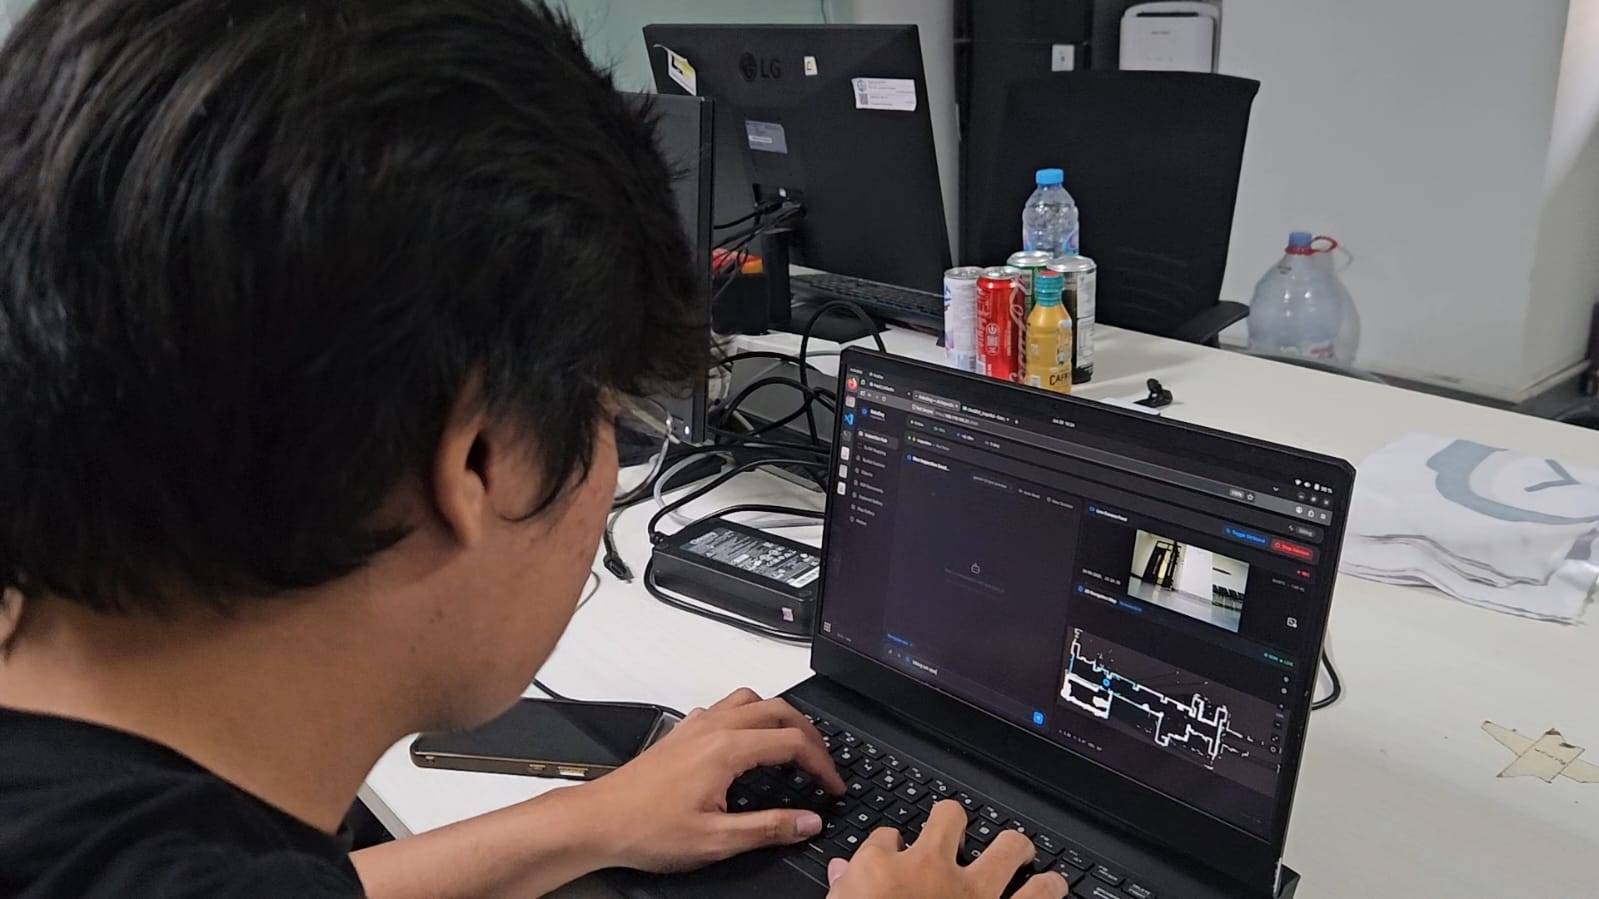
\includegraphics[width=0.8\textwidth]{Init/gambar/responden.jpeg}
    \caption{Dokumentasi Pelaksanaan Pengujian NASA-TLX oleh Responden}
    \label{fig:dokumentasi_responden}
\footnotesize \textbf{Sumber:} Dokumentasi Penulis
\end{figure}

\begin{table}[H]
\centering
\caption{Profil Demografi Responden NASA-TLX}
\label{tab:profil_responden}
\begin{tabular}{|c|l|c|c|l|l|}
\hline
\textbf{No} & \textbf{Nama} & \textbf{Usia} & \textbf{Gender} & \textbf{Pengalaman Robot} & \textbf{Familiaritas AI} \\
\hline
1 & Responden 1 & 21 & L & Pemula & Sangat Familiar \\
\hline
2 & Responden 2 & 22 & P & Pemula & Sangat Familiar \\
\hline
3 & Responden 3 & 22 & L & Pemula & Cukup Familiar \\
\hline
4 & Responden 4 & 22 & L & Tidak Pernah & Cukup Familiar \\
\hline
5 & Responden 5 & 21 & L & Tidak Pernah & Sangat Familiar \\
\hline
6 & Responden 6 & 19 & P & Pemula & Sangat Familiar \\
\hline
7 & Responden 7 & 19 & P & Pemula & Cukup Familiar \\
\hline
8 & Responden 8 & 20 & L & Pemula & Sangat Familiar \\
\hline
9 & Responden 9 & 22 & L & Tidak Pernah & Sangat Familiar \\
\hline
10 & Responden 10 & 22 & L & Tidak Pernah & Sangat Familiar \\
\hline
\end{tabular}
\end{table}

\subsection{Hasil Pengujian}

\begin{table}[H]
\centering
\caption{Skor NASA-TLX per Responden untuk Setiap Kondisi Inspeksi}
\label{tab:nasa_tlx_scores}
\begin{tabular}{|c|c|c|c|}
\hline
\textbf{Responden} & \textbf{Manual} & \textbf{Nav. Otomatis} & \textbf{Full Otomatis} \\
\hline
1 & 72,67 & 50,00 & 38,67 \\
\hline
2 & 45,33 & 43,00 & 19,67 \\
\hline
3 & 45,33 & 12,33 & 5,00 \\
\hline
4 & 23,33 & 41,67 & 2,67 \\
\hline
5 & 43,33 & 26,00 & 12,67 \\
\hline
6 & 75,67 & 42,33 & 35,33 \\
\hline
7 & 48,33 & 54,67 & 11,33 \\
\hline
8 & 80,00 & 26,67 & 23,00 \\
\hline
9 & 91,33 & 43,67 & 13,33 \\
\hline
10 & 16,00 & 5,33 & 22,33 \\
\hline
\hline
\textbf{Rata-rata} & \textbf{54,13} & \textbf{34,57} & \textbf{18,40} \\
\hline
\end{tabular}
\end{table}

\begin{figure}[H]
    \centering
    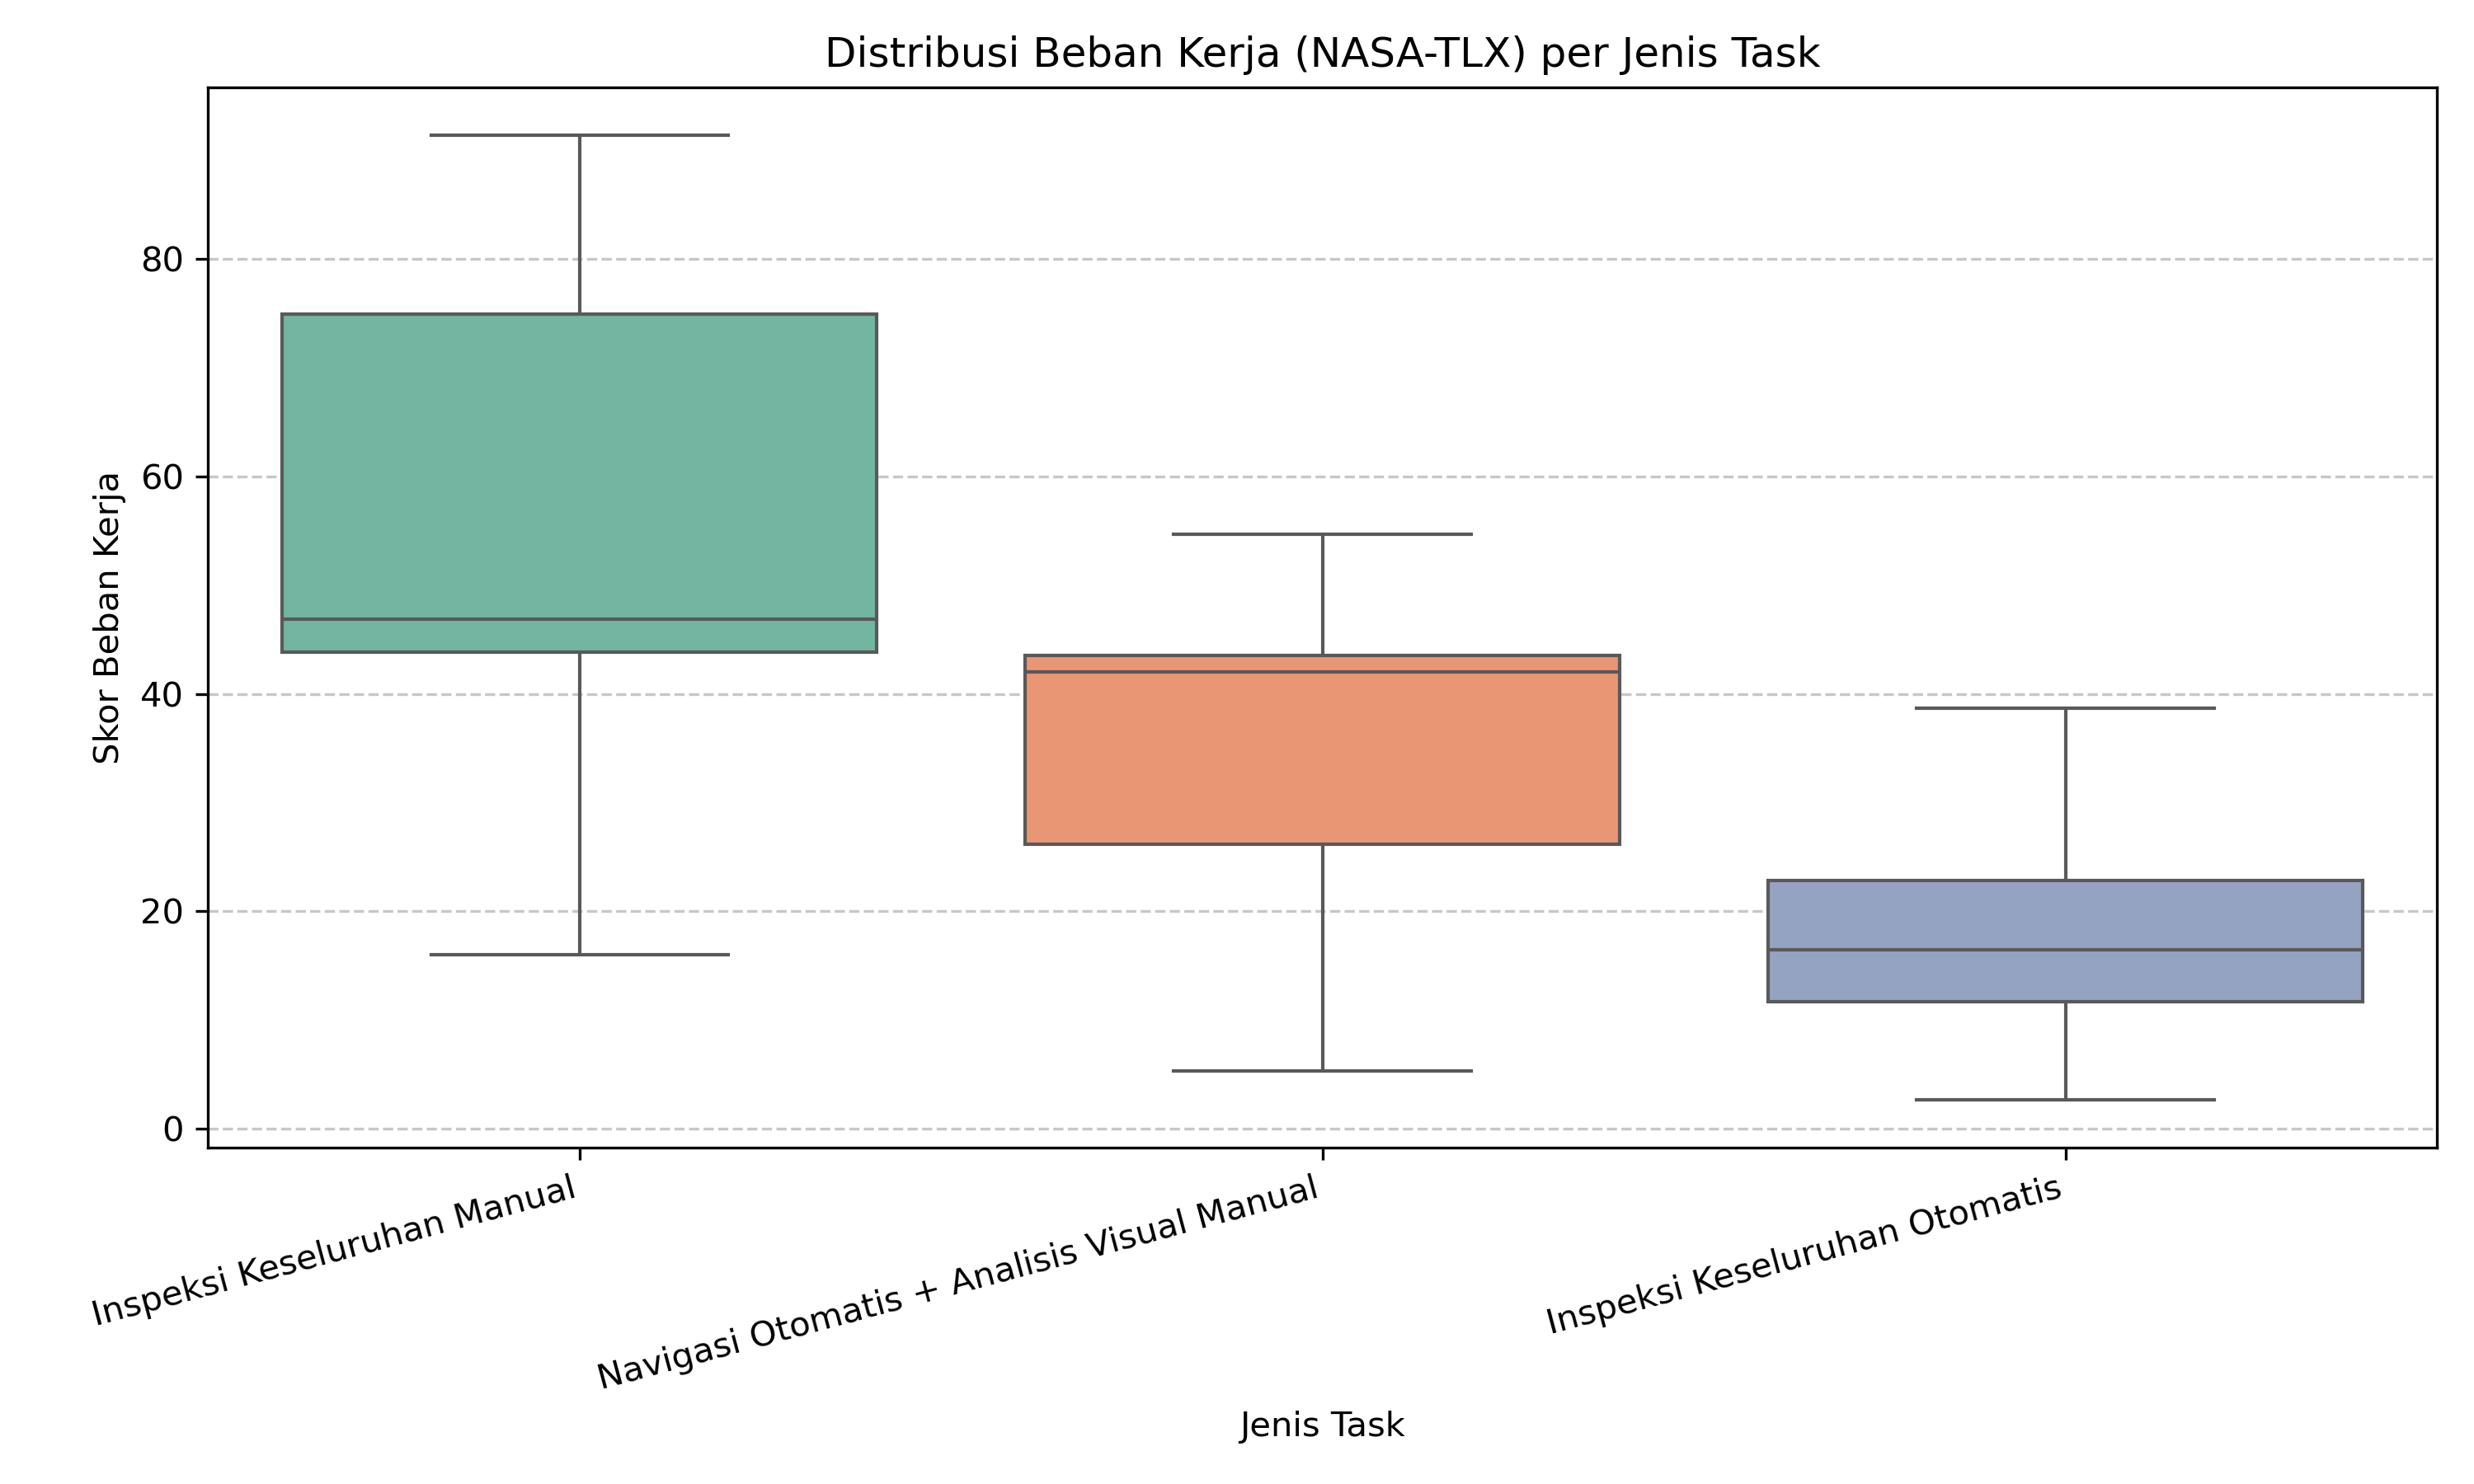
\includegraphics[width=0.8\textwidth]{Init/gambar/boxplots/boxplot_nasa_tlx.png}
    \caption{Distribusi Skor NASA-TLX untuk Tiga Kondisi Inspeksi}
    \label{fig:boxplot_nasa_tlx}
\footnotesize \textbf{Sumber:} Dokumentasi Penulis
\end{figure}

\subsection{Analisis Hasil}

Berdasarkan distribusi skor NASA-TLX yang divisualisasikan melalui \textit{boxplot} pada \textit{image} \ref{fig:boxplot_nasa_tlx} serta hasil pengujian yang disajikan pada Tabel \ref{tab:nasa_tlx_scores}, sistem inspeksi cerdas yang dikembangkan berhasil secara signifikan menurunkan beban kerja operator. Terlihat tren penurunan rata-rata skor beban kerja yang konsisten seiring dengan peningkatan level otonomi, dari 54,13 pada mode Inspeksi Keseluruhan Manual, turun menjadi 34,57 pada mode Navigasi Otomatis, dan mencapai titik terendah 18,40 pada mode Inspeksi Full Otomatis. Sistem ini berhasil menggeser kategori beban kerja operator dari level tinggi (\textit{High}) pada mode teleoperasi manual, menjadi level sedang (\textit{Medium}) saat robot menavigasi dirinya sendiri, hingga mencapai level rendah (\textit{Low}) ketika seluruh proses analisis visual juga diotomatisasi oleh MLLM.

Penurunan beban kerja secara umum bersumber pada reduksi tuntutan fisik dan mental. Pada mode manual, operator dituntut secara fisik untuk mengendalikan \textit{joystick} dan fokus menjaga kewaspadaan spasial dari kamera robot agar tidak menabrak halangan. Transisi ke navigasi otomatis mendelegasikan tugas gerak tersebut ke \textit{ROS Navigation Stack}, sehingga usaha fisik dan waktu yang dibutuhkan berkurang drastis. Selanjutnya, transisi ke mode full otomatis membebaskan operator dari kewajiban memproses dan mengklasifikasikan anomali objek secara kognitif, yang pada akhirnya meminimalisasi \textit{Mental Demand} dan \textit{Frustration Level}.

Kendati tren rata-rata secara keseluruhan menunjukkan penurunan beban kerja, analisis pada data individu mengungkap adanya beberapa anomali di mana beban kerja justru dirasakan meningkat pada mode otomatis. Anomali ini dipicu oleh dua faktor utama, yaitu faktor teknis dan psikologis. Dari segi teknis, kegagalan fungsi sistem saat uji coba lapangan, seperti disfungsi navigasi robot di lintasan atau kesalahan MLLM dalam menganalisis kondisi objek, secara langsung merusak persepsi kesuksesan misi. Kondisi ini mendorong operator untuk memberikan penalti skor yang berat pada dimensi Performansi (\textit{Performance}) dan Kebutuhan Waktu (\textit{Temporal Demand}). Sementara itu dari sisi psikologis, pergeseran peran dari pengendali aktif menjadi pengawas pasif pada tahap awal transisi otomatisasi sering kali memunculkan kecemasan. Operator yang belum sepenuhnya membangun rasa percaya terhadap sistem cenderung melakukan pengawasan berlebih. Hal ini justru membebani mereka secara mental dan menuntut usaha yang terkadang dirasa lebih melelahkan daripada mengendalikan robot secara langsung.


\cleardoublepage
\chapter{PENUTUP}
\label{sec:chap5_tutup}
\vspace{1ex}

\section{Kesimpulan}
Berdasarkan hasil perancangan, implementasi, dan pengujian sistem inspeksi otonom berbasis \textit{Agentic} AI terintegrasi \textit{Multimodal Large Language Model} yang telah dilakukan, dapat ditarik kesimpulan yang menjawab tujuan penelitian sebagai berikut:

\begin{enumerate}
    \item Integrasi MLLM telah berhasil menangani skenario inspeksi yang berbeda, baik dari segi perbedaan rute maupun variasi objek target, secara adaptif tanpa perubahan kode. Melalui MCP, instruksi bahasa alami dari pengguna berhasil diterjemahkan secara otomatis menjadi pemanggilan \textit{tools} pergerakan fisik robot serta analisis visual berbasis dokumen SOP. Pada pengujian \textit{end-to-end} terhadap 9 skenario misi bertingkat yang mencakup 30 titik inspeksi, Gemini 3.1 Pro Preview mencatatkan kinerja terbaik dengan akurasi analisis visual sebesar 93,33\% (28/30), efisiensi rute \textit{plan} 100\% (9/9), dan rata-rata latensi waktu sesi 6.1 menit. Gemini 2.5 Flash menyusul di posisi kedua dengan akurasi analisis visual 86,67\% (26/30), efisiensi rute 77,78\% (7/9), dan rata-rata latensi waktu sesi 6.4 menit. Sementara itu, model lokal Qwen 3.5 27B mencatatkan akurasi visual 63,33\% (19/30) dan efisiensi rute 66,67\% (6/9) dengan rata-rata latensi waktu sesi paling tinggi mencapai 10.2 menit (bahkan mencapai 17 hingga 26 menit pada level sulit), sehingga model lokal kurang efektif dibanding model \textit{cloud}. Keberhasilan integrasi MLLM, terutama pada model Gemini 3.1 Pro Preview, terbukti memangkas total beban kerja operator (NASA-TLX) secara signifikan dari 54,13 (pada kendali manual) menjadi 18,40.
    
    \item Arsitektur \textit{Human-in-the-Loop} dengan mekanisme eksekusi bertahap sukses diimplementasikan dan mampu membuat sistem beradaptasi di tengah berjalannya misi. Sistem umpan balik otomatis memungkinkan robot untuk menginformasikan bahwa robot telah mencapai setiap titik koordinat dan meminta validasi lanjutan. Pengujian terhadap 4 skenario intervensi yang berbeda (perubahan rencana awal, penambahan objek di tengah misi, pembatalan dan penggantian objek, serta gerakan tambahan manual) menunjukkan bahwa seluruh model MLLM yang diuji mencapai keberhasilan dalam mengakomodasi setiap jenis intervensi tersebut pada cakupan skenario yang dirancang. Meskipun demikian, variasi intervensi yang diuji masih terbatas pada empat pola dasar, sehingga keberhasilan ini belum dapat digeneralisasi untuk seluruh kemungkinan intervensi di lingkungan operasional yang lebih kompleks.
\end{enumerate}

\section{Saran}
Penelitian ini telah meletakkan fondasi arsitektur agen inspeksi otonom yang interaktif, namun masih terdapat ruang untuk pengembangan lebih lanjut. Beberapa saran yang dapat dipertimbangkan untuk penelitian di masa mendatang meliputi:

\begin{enumerate}
    \item Penggunaan teknik \textit{context pruning} (pemangkasan riwayat) dan peringkasan memori untuk menjaga stabilitas kecepatan inferensi MLLM lokal tanpa mengorbankan akurasi historis.
    
    \item Eksplorasi model lokal lain, terutama VLN (\textit{Vision-Language Navigation}) seperti Qwen-RobotNav, yang dirancang khusus untuk penalaran spasial dan navigasi otonom.
    
    \item Melakukan migrasi dari ROS Noetic ke ROS 2 Humble untuk memanfaatkan \textit{Navigation Stack} yang lebih canggih.
    
    \item Memperluas cakupan pengujian dengan menambah jumlah iterasi, variasi jenis objek inspeksi, kompleksitas lingkungan operasional, serta pola intervensi operator yang lebih beragam untuk menguji batas kemampuan sistem secara lebih komprehensif.
\end{enumerate}

\cleardoublepage
\input{Init/DaftarPustaka.tex}
\cleardoublepage
\begin{center}
  \Large
  \textbf{BIOGRAFI PENULIS}
\end{center}

\addcontentsline{toc}{chapter}{BIOGRAFI PENULIS}

\vspace{2ex}

\begin{wrapfigure}{L}{0.3\textwidth}
  \centering
  \vspace{-3ex}
  % Ubah file gambar berikut dengan file foto dari mahasiswa
  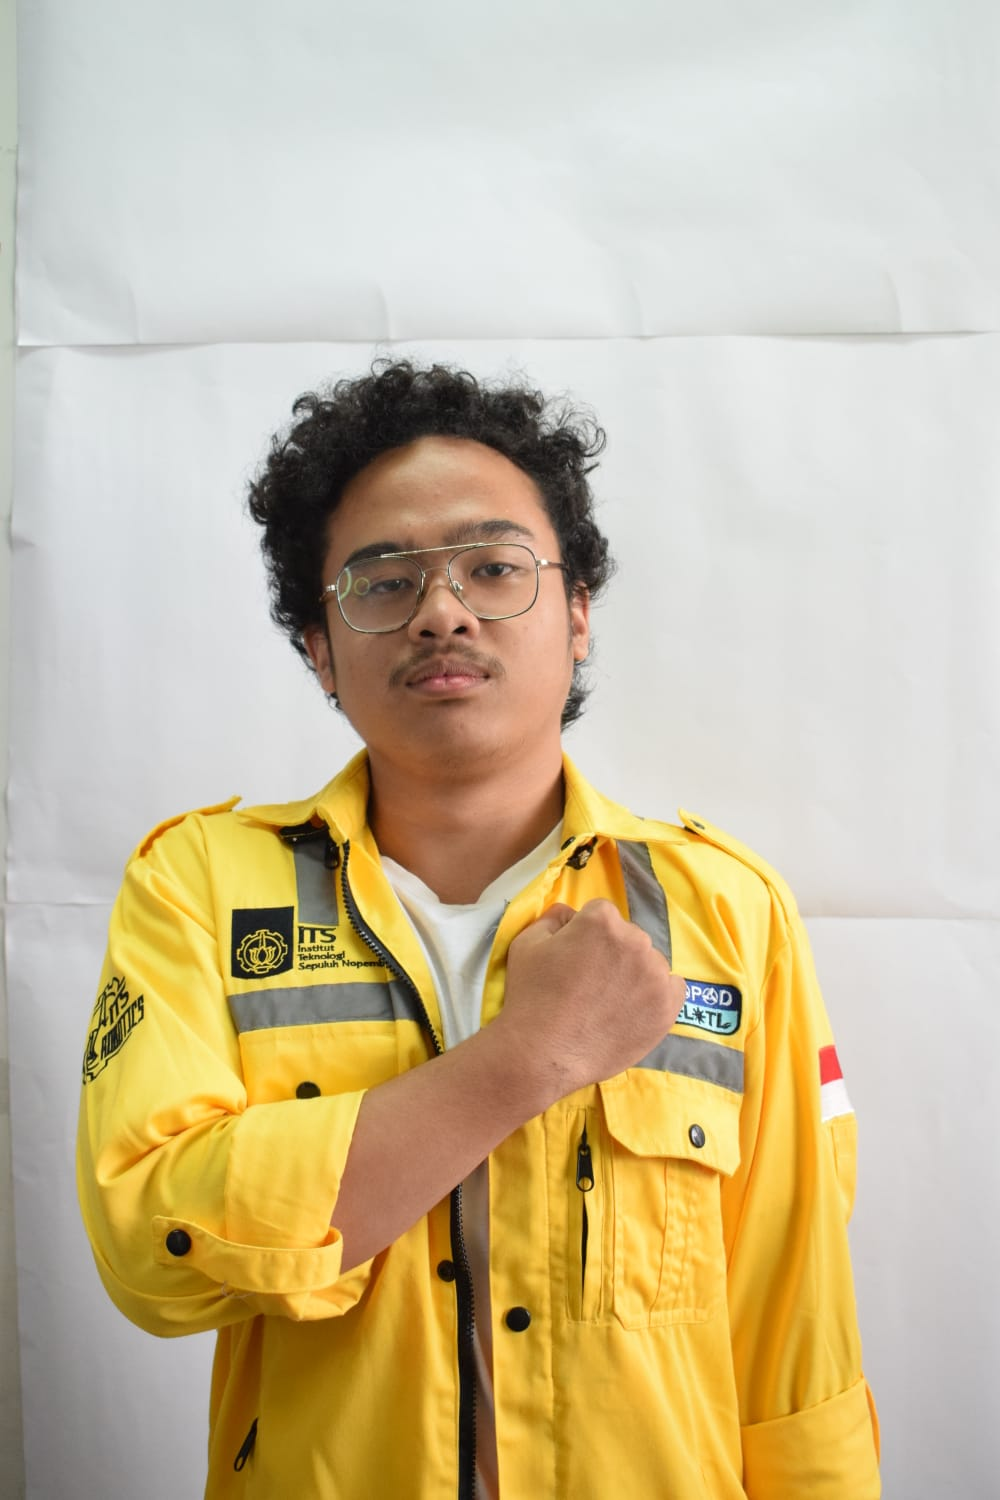
\includegraphics[width=0.3\textwidth]{BiografiPenulis/foto.jpeg}
  \vspace{-4ex}
\end{wrapfigure}

% Ubah kalimat berikut dengan biografi dari mahasiswa
Penulis bernama \name{}, lahir di Sukabumi pada tanggal 14 Februari 2004. Penulis menempuh pendidikan terakhir di SMA Pesantren Unggul AL-Bayan. Ketertarikan penulis terhadap dunia teknologi telah mendorongnya untuk mendalami bidang robotika, kecerdasan buatan. Pada tahun 2022, penulis melanjutkan pendidikan tinggi pada Program Studi Sarjana (S1) Teknik Komputer, Departemen Teknik Komputer, Fakultas Teknologi Elektro dan Informatika Cerdas, Institut Teknologi Sepuluh Nopember (ITS).

Selama masa studi di perguruan tinggi, penulis merupakan mahasiswa yang sangat aktif dan berprestasi, baik dalam riset, kompetisi, maupun pengembangan karier profesional. Penulis tergabung sebagai staf ahli divisi pemrograman dalam tim riset robot bawah air Banyubramanta ITS. Bersama tim ini, penulis turut berkontribusi dalam merancang kontrol dan sistem otonom AUV yang membuahkan hasil membanggakan, di antaranya Juara 1 Nasional Kontes Robot Bawah Air Indonesia (KRBAI) 2024 dan Juara 1 MATE ROV ASEAN 2023.

Di luar lingkup kompetisi, penulis juga aktif mengasah keterampilan teknisnya melalui program magang sebagai \emph{AI Engineer Intern} di PT. Altimeda Cipta Visitama, serta memimpin pengembangan Web pada ITS EXPO 2023, serta berkontribusi dalam pengembangan website pada acara MAGE X. Penga\-laman-penga\-laman ini memperkuat keahlian pengembangan perangkat lunaknya, dengan fokus pada membangun sistem backend yang skalabel dan efisien. 

% Penulis saat ini sedang menyusun Tugas Akhir (TA) berjudul ``SISTEM INSPEKSI VISUAL PADA ROBOT \textit{QUADRUPED} BERBASIS \textit{LARGE LANGUAGE MODEL} DENGAN MEKANISME \textit{HU\-MAN-IN-THE-LOOP}'', sebuah inovasi yang mengintegrasikan \textit{Large Language Model} melalui standar \textit{Model Context Protocol} (MCP) untuk memampukan sistem inspeksi dengan penalaran berbasis semantik dalam operasionalnya. Melalui penelitian tersebut, penulis berharap dapat memberikan kontribusi signifikan terhadap perkembangan teknologi robotika berbasis AI di Indonesia. Bagi pembaca yang tertarik untuk berdiskusi, penulis dapat dihubungi melalui email \url{muhamadrizanoalamsyah@gmail.com}.
\cleardoublepage
\end{document}
